% !Mode:: "TeX:UTF-8"
\PassOptionsToPackage{}{graphicx}
\documentclass[doctor,openright,twoside,AutoFakeBold=true]{buaathesis}

% 参考文献
\usepackage{gbt7714}
% 参考文献输出方式,numerical为按照出现顺序,authoryear为按照作者姓名和年份
\citestyle{numerical}
% \citestyle{authoryear}

\makeatletter

%%%%%%%%%%%%%%%%%%%%%%%%%%%%%% LyX specific LaTeX commands.
\newcommand{\noun}[1]{\textsc{#1}}
\long\def\lyxmintcaption[#1]#2{%
	\ifx#1t\vskip\baselineskip\fi%
	\refstepcounter{listing}\noindent%
	\addcontentsline{lol}{listing}%
	{\protect\numberline{\thelisting}{\ignorespaces #2}}%
	\setbox\@tempboxa\hbox{\listingscaption~\thelisting: #2}%
	\ifdim \wd\@tempboxa >\linewidth%
	\parbox[t]{\linewidth}{\unhbox\@tempboxa}\else%
	\hbox to\linewidth{\hfil\box\@tempboxa\hfil}\fi%
	\ifx#1b\vskip\baselineskip\fi
}
\AtBeginDocument{
	\renewcommand{\listingscaption}{代码片段}
	\renewcommand{\listoflistingscaption}{代码目录}
}

%%%%%%%%%%%%%%%%%%%%%%%%%%%%%% Textclass specific LaTeX commands.
\makeatletter

\theoremstyle{plain}
\ifx\thechapter\undefined
\newtheorem{thm}{\protect\theoremname}
\else
\newtheorem{thm}{\protect\theoremname}[chapter]
\fi
\theoremstyle{definition}
\newtheorem{defn}[thm]{\protect\definitionname}
\theoremstyle{plain}
\newtheorem{lem}[thm]{\protect\lemmaname}
\theoremstyle{plain}
\newtheorem{cor}[thm]{\protect\corollaryname}
\theoremstyle{remark}
\newtheorem{rem}[thm]{\protect\remarkname}
\theoremstyle{remark}
\newtheorem*{rem*}{\protect\remarkname}
\theoremstyle{definition}
\newtheorem*{example*}{\protect\examplename}
\theoremstyle{plain}
\newtheorem{lyxalgorithm}[thm]{\protect\algorithmname}
\theoremstyle{definition}
\newtheorem{example}[thm]{\protect\examplename}
\theoremstyle{plain}
\newtheorem*{assumption*}{\protect\assumptionname}
\theoremstyle{plain}
\newtheorem{ax}[thm]{\protect\axiomname}
\theoremstyle{remark}
\newtheorem*{notation*}{\protect\notationname}
\theoremstyle{plain}
\newtheorem*{thm*}{\protect\theoremname}
\theoremstyle{definition}
\newtheorem*{defn*}{\protect\definitionname}
\theoremstyle{remark}
\newtheorem{notation}[thm]{\protect\notationname}
\theoremstyle{plain}
\newtheorem{conjecture}[thm]{\protect\conjecturename}
\theoremstyle{remark}
\newtheorem*{claim*}{\protect\claimname}
\theoremstyle{definition}
\newtheorem*{sol*}{\protect\solutionname}
\theoremstyle{plain}
\newtheorem{fact}[thm]{\protect\factname}
\theoremstyle{plain}
\newtheorem*{cor*}{\protect\corollaryname}
\theoremstyle{definition}
\newtheorem{problem}[thm]{\protect\problemname}
\theoremstyle{plain}
\newtheorem*{lem*}{\protect\lemmaname}
\theoremstyle{plain}
\newtheorem{assumption}[thm]{\protect\assumptionname}
\theoremstyle{definition}
\newtheorem{condition}[thm]{\protect\conditionname}

\AddToHook{env/problem/begin}{\pushQED{\qed}}
\AddToHook{env/problem/end}{\popQED}

\def\th@plain{ \songti }
\def\th@definition{ \songti }

\makeatother

\usepackage[intoc]{nomencl}
\makenomenclature
\renewcommand{\nomname}{主要符号对照表}

\usepackage[chapter]{minted}
\setminted{style=xcode,
	frame=leftline,
	baselinestretch={1.2},
	breaklines=true,
	fontsize={\normalsize}
}

\providecommand{\algorithmname}{算法}
\providecommand{\assumptionname}{假设}
\providecommand{\axiomname}{公理}
\providecommand{\claimname}{声明}
\providecommand{\conditionname}{条件}
\providecommand{\conjecturename}{猜想}
\providecommand{\corollaryname}{推论}
\providecommand{\definitionname}{定义}
\providecommand{\examplename}{例}
\providecommand{\factname}{事实}
\providecommand{\lemmaname}{引理}
\providecommand{\notationname}{记号}
\providecommand{\problemname}{问题}
\providecommand{\remarkname}{注}
\providecommand{\solutionname}{解答}
\providecommand{\theoremname}{定理}
%
% Settings for Graphics
%
\usepackage{tikz}
\usetikzlibrary{intersections}
\usetikzlibrary{arrows.meta}
\usetikzlibrary{angles}
\usetikzlibrary{calc}
\usetikzlibrary{quotes}

\usepackage{diagbox}

%%%%%%%%%%%%%%%%%%%%%%%%%%%%%% User specified LaTeX commands.

\usepackage{tablefootnote}
\usepackage{physics}
\usepackage{unicode-math}
\setsansfont[
ItalicFont=NewCMSans10-BookOblique,
BoldFont=NewCMSans10-Bold,
BoldItalicFont=NewCMSans10-BoldOblique,
SmallCapsFeatures={Numbers=OldStyle}
]{NewCMSans10-Book}
\setmonofont[
ItalicFont=NewCMMono10-BookItalic,
BoldFont=NewCMMono10-Bold,
BoldItalicFont=NewCMMono10-BoldOblique,
SmallCapsFeatures={Numbers=OldStyle}
]{NewCMMono10-Book}
\setmathfont{NewCMMath-Book}[
	math-style = ISO,
	bold-style = ISO,
]
\setmathfont{Times New Roman}[
	range = {up/{num, latin}}
]
\AtBeginDocument{
	\newcommand{\Mat}[1]{\mathinner{\underline{#1}}}
	\renewcommand{\vdot}{\mathbin{\mdsmblkcircle}}
	\renewcommand{\cross}{\vectimes}
	\renewcommand{\emptyset}{\diameter}
	\renewcommand{\varnothing}{\diameter}
	%% italic versions of the capital Greek letters
	\let\oldGamma\Gamma
	\let\oldGamma\Gamma
	\let\oldDelta\Delta
	\let\oldTheta\Theta
	\let\oldLambda\Lambda
	\let\oldXi\Xi
	\let\oldPi\Pi
	\let\oldSigma\Sigma
	\let\oldUpsilon\Upsilon
	\let\oldPhi\Phi
	\let\oldPsi\Psi
	\let\oldOmega\Omega
	\renewcommand{\Gamma}{\symup{\oldGamma}}
	\renewcommand{\Delta}{\symup{\oldDelta}}
	\renewcommand{\Theta}{\symup{\oldTheta}}
	\renewcommand{\Lambda}{\symup{\oldLambda}}
	\renewcommand{\Xi}{\symup{\oldXi}}
	\renewcommand{\Pi}{\symup{\oldPi}}
	\renewcommand{\Sigma}{\symup{\oldSigma}}
	\renewcommand{\Upsilon}{\symup{\oldUpsilon}}
	\renewcommand{\Phi}{\symup{\oldPhi}}
	\renewcommand{\Psi}{\symup{\oldPsi}}
	\renewcommand{\Omega}{\symup{\oldOmega}}
	\renewcommand{\varGamma}{\mitGamma}
	\renewcommand{\varDelta}{\mitDelta}
	\renewcommand{\varTheta}{\mitTheta}
	\renewcommand{\varLambda}{\mitLambda}
	\renewcommand{\varXi}{\mitXi}
	\renewcommand{\varPi}{\mitPi}
	\renewcommand{\varSigma}{\mitSigma}
	\renewcommand{\varUpsilon}{\mitUpsilon}
	\renewcommand{\varPhi}{\mitPhi}
	\renewcommand{\varPsi}{\mitPsi}
	\renewcommand{\varOmega}{\mitOmega}
	\renewcommand{\mathrm}[1]{\symup{#1}}
	\renewcommand{\mathbf}[1]{\symbf{#1}}
	\renewcommand{\boldsymbol}[1]{\symbf{#1}}
}
\usepackage{cancel}
\usepackage{siunitx}
% `physics` and `unicode-math` treat `\div` differently:
\let\divg\divergence  % define another abbr for `\divergence`.

%\AtBeginEnvironment{tabular}{\linespread{1.0}\selectfont}
\renewcommand{\thefootnote}{(\alph{footnote})}

\usepackage{subfig}

\begin{document}

% 用户信息
% !Mode:: "TeX:UTF-8"

% 学院中英文名,中文不需要“学院”二字
% 院系英文名可从以下导航页面进入各个学院的主页查看
% https://www.buaa.edu.cn/jgsz/yxsz.htm
\school
{航空科学与工程}{School of Aeronautic Science and Engineering}

% 专业中英文名
\major
{飞行器设计}{Aircraft Design}

% 论文中英文标题
\thesistitle
{舰载直升机气动干扰\\计算方法研究}
{}
{Study on Computational Method for Aerodynamic Interference of Shipborne Helicopters}
{}

% 作者中英文名
\thesisauthor
{裴为诚}{Pei Weicheng}

% 导师中英文名
\teacher
{李书}{Li Shu}
% 副导师中英文名
% 注:慎用‘副导师’,见北航研究生毕业论文规范
%\subteacher{(副导师姓名)}{(Name of Subteacher)}

% 中图分类号,可在 http://www.ztflh.com/ 查询
\category{V275}

% 本科生为毕设开始时间;研究生为学习开始时间
\thesisbegin{2014}{09}{\phantom{01}}

% 本科生为毕设结束时间;研究生为学习结束时间
\thesisend{2022}{08}{\phantom{31}}

% 毕设答辩时间
\defense{2022}{08}{08}

% 中文摘要关键字
\ckeyword{舰载直升机,气动干扰,旋翼空气动力学,间断伽辽金有限元法,加权基本无振荡重构,非定常动量源模型}

% 英文摘要关键字
\ekeyword{shipborne helicopter, aerodynamic interference, rotor aerodynamics, discontinuous Galerkin (DG) finite element method, weighted essentially non-oscillatory (WENO) reconstruction, unsteady momentum source (UMS) model}

% !Mode:: "TeX:UTF-8"

% 研究方向
\direction{直升机气动、计算力学}

% 导师职称中英文
\teacherdegree{教授}{Professor}
% 副导师职称中英文
% 注:慎用‘副导师’,见北航研究生毕业论文规范
%\subteacherdegree{(副导师职称)}{(Subteacher Degree)}

% 保密等级 保密期限,注:非保密论文时不需要此项
%\mibao{(保密等级)}{(保密期限)}

%申请学位级别
\applydegree{博士}

% 论文编号,由10006+学号组成
\thesisID{10006BY1405156}

% 论文提交时间
\commit{2022}{07}{15}

% 学位授予日期
\award{2022}{11}{\phantom{08}}

% 中英封面、提名页、授权书
\maketitle
% 前言页眉页脚样式
\pagestyle{frontmatter}
% 摘要
% !Mode:: "TeX:UTF-8"

% 中英文摘要
\phantomsection
\addcontentsline{toc}{chapter}{摘要}
\begin{cabstract}
舰载直升机空气动力学以旋翼空气动力学为基础,侧重于研究旋翼与船体及海面之间的气动干扰问题。
随着计算机硬件性能的提高,特别是高性能计算平台的普及,数值计算正日益成为研究包括舰载直升机气动干扰在内的复杂工程物理问题的重要手段。
舰载直升机气动干扰的计算难点,主要来源于旋翼对流场的非定常扰动,其次来源于船体的复杂几何外形。

现有的旋翼空气动力学数值方法,要么基于简化的物理模型,如:自由尾迹模型、涡粒子模型;要么基于动态网格技术,如:变形网格、滑动网格、重叠网格。
前者计算效率虽高,但对于固体壁面通常以镜像法做处理,难以处理具有复杂几何外形的流场边界,从而不适合用于研究舰载直升机气动干扰问题。
后者虽能处理几何外形更复杂的固体边界,但频繁重构网格,或者在不同网格之间频繁交换数据,所增加的计算成本都是日常研究难以承受的。

本文的主要目标是提供一种既能处理复杂船体外形,又能在较粗的非结构网格上保持较高精度,还能在静态网格上高效地捕捉旋翼对流场非定常扰动的计算方法。
为此,本文的主要内容包括:
\begin{enumerate}[wide]
\item 提出一种适用于舰载直升机流场计算的高阶数值方法。该方法以间断伽辽金有限元为空间离散方法,以保持强稳定性的龙格--库塔格式做显式时间推进,以非定常动量源模型表示桨叶对流场的非定常扰动,以加权基本无振荡重构技术压制桨叶附近的数值振荡。
\item 利用具有解析解或数值精确解的一维标准算例,定量验证上述高阶数值方法的正确性和精度阶数;利用拥有公认数值解的二维标准算例,定性验证上述高阶数值方法捕捉复杂流动图象的能力。
\item 在此基础上,以数学上等价于经典有限体积解、物理上较为可靠的一阶近似解为参照,定性验证三阶近似解的正确性和精度优势。
\item 提出并实现一种上述高阶数值方法的分布式并行加速方案,在实验室自建的小型机群上测量加速比和并行效率。
\item 将上述并行化的高阶数值方法,应用到舰载直升机气动干扰问题的研究中。
\end{enumerate}

本文以舰载直升机气动干扰问题为研究对象,
提出了一种支持分布式并行计算的动量源--高阶有限元混合方法,
为舰载直升机气动干扰问题的研究,提供了一种高效且具有高阶精度的数值计算工具。
\newpage{}
\end{cabstract}

\begin{eabstract}
Based on rotor aerodynamics, shipborne helicopter aerodynamics focuses on the aerodynamic interference between the rotor, the hull and the sea surface.
With the improvement of computer hardware performance, especially the popularization of high-performance computing platforms, numerical computing is increasingly becoming an important research method for complex engineering physics problems including the aerodynamic interference of shipborne helicopters.
The difficulty in calculating the aerodynamic interference of shipborne helicopters mainly comes from the unsteady disturbance of the rotor to the flow field, and secondly from the complex geometric shape of the hull.

Existing numerical methods of rotor aerodynamics are either based on simplified physical models, such as the free wake model and the vortex particle model; or based on dynamic mesh technology, such as deformed mesh, sliding mesh, and overlapping mesh.
Although the former has high computational efficiency, solid walls are usually handled by the mirror method, which is difficult to deal with the flow field boundary with complex geometric shapes, so it is not suitable for studying the aerodynamic interference problem of shipborne helicopters.
Although the latter can handle solid boundaries with more complex geometric shapes, frequent mesh reconstruction or frequent exchange of data between different meshes results in an unbearable computational cost for daily research.

The main goal of this thesis is to provide a computational method that can handle complex hull shapes, maintain high accuracy on coarse unstructured grids, and efficiently capture rotor unsteady disturbances to flow fields on static grids.
To this end, the main contents of this thesis include:
\begin{enumerate}[wide]
\item Propose a high-order numerical method suitable for the computation of the flow field of shipborne helicopters. In this method, the discontinuous Galerkin finite element method is used as the spatial discretization method, the Runge--Kutta scheme which is strong stability preserving is used for explicit time marching, and an unsteady momentum source model is used to represent the unsteady disturbance of the blade to the flow field. Numerical oscillations near the blade are suppressed by a weighted essentially non-oscillatory reconstruction technique.
\newpage{}
\item Quantitatively verify the correctness and order of accuracy of the above high-order numerical methods using one-dimensional standard examples with analytical solutions or numerically accurate solutions. Qualitatively verify the above high-order numerical methods using two-dimensional standard examples with recognized numerical solutions. The method's ability to capture complex flowing images.
\item On this basis, taking the mathematically equivalent to the classical finite volume solution and the physically reliable first-order approximate solution as a reference, the correctness and precision advantages of the third-order approximate solution are qualitatively verified.
\item Propose and implement a distributed parallel acceleration scheme of the above-mentioned high-order numerical method, and measured the speedup ratio and parallel efficiency on a small cluster built by the laboratory.
\item Apply the above parallelized high-order numerical method to the study of the aerodynamic interference problem of shipborne helicopters.
\end{enumerate}

This thesis takes the aerodynamic interference problem of shipborne helicopters as the research object.
A momentum source--high-order finite element hybrid method, which supports distributed parallel computing, is proposed.
An efficient tool with high-order accuracy is provided for the study of aerodynamic interference of shipborne helicopters.
\end{eabstract}
% 目录、插图目录、表格目录
\phantomsection
\addcontentsline{toc}{chapter}{目录}
\tableofcontents

\begingroup

\renewcommand\citet[2][]{}
\renewcommand\cite[2][]{}
\renewcommand\upcite[2][]{}

\cleardoublepage
\phantomsection
\addcontentsline{toc}{chapter}{插图目录}
\listoffigures

\cleardoublepage
\phantomsection
\addcontentsline{toc}{chapter}{表格目录}
\listoftables

\endgroup
% 符号表
\printnomenclature

% 正文页码样式
\mainmatter
% 正文页眉页脚样式
\pagestyle{mainmatter}

% 正文

\chapter{绪论\label{chap:=007EEA=008BBA}}

\section{研究背景和意义}

直升机以其特有的垂直起降、悬停和低空低速飞行能力,特别适合于在军舰、科考船、海上钻井平台等飞行环境较差的起降平台上执行任务。舰载直升机能够有效扩大船舶作业半径、丰富海上作业科目、提升应对海上突发情况的能力。发展舰载直升机对于保障船舶航行安全、维护海洋权益具有重要意义。世界各海洋大国和航空大国历来重视舰载直升机的发展,相继研制出各种不同构型的舰载直升机,如表
\ref{tab:shipborne-helicopter} 所示。当前,人民海军正处于“近海防御型向近海防御与远海护卫型结合转变”\upcite{PRC2015}的关键时期。发展适合我国国情的舰载直升机,对于海洋强国战略的实施具有重要意义。
\begin{table}
\caption{\label{tab:shipborne-helicopter}国外主要舰载直升机}

\begin{longtable}[c]{cccccc}
\toprule 
首飞时间 & 研制单位 & 型号 & 别名/绰号 & 构型 & 旋翼直径 (m)\tabularnewline
\midrule
1954 & 美国西科斯基公司 & UH-34D/E & Sea Horse & 单旋翼带尾桨式 & 17.07\tabularnewline
1959 & 美国西科斯基公司 & SH-3A & Sea King & 单旋翼带尾桨式 & 18.9\tabularnewline
1959 & 美国卡曼宇航公司 & SH-2 & Sea Sprite & 单旋翼带尾桨式 & 13.14\tabularnewline
1961 & 苏联卡莫夫设计局 & Ka-25 & Hormone & 双旋翼共轴式 & 15.74\tabularnewline
1962 & 美国波音直升机公司 & CH-46 & Sea Knight & 双旋翼纵列式 & 15.24\tabularnewline
1963 & 法国宇航公司 & SA321 & Super Frelon & 单旋翼带尾桨式 & 18.9\tabularnewline
1964 & 美国西科斯基公司 & CH-53A & Sea Stallion & 单旋翼带尾桨式 & 22.02\tabularnewline
1966 & 美国贝尔直升机公司 & TH-57A/B/C & Sea Ranger & 单旋翼带尾桨式 & 10.16\tabularnewline
1973 & 苏联卡莫夫设计局 & Ka-27/28 & Helix & 双旋翼共轴式 & 15.9\tabularnewline
1976 & 苏联卡莫夫设计局 & Ka-29 & Helix-B & 双旋翼共轴式 & 15.9\tabularnewline
1978 & 法国宇航公司 & AS332/AS532 & Super Puma & 单旋翼带尾桨式 & 15.6\tabularnewline
1979 & 美国西科斯基公司 & SH-60B & Sea Hawk & 单旋翼带尾桨式 & 12.74\tabularnewline
1981 & 苏联卡莫夫设计局 & Ka-32 & Helix-C & 双旋翼共轴式 & 15.9\tabularnewline
1982 & 法国宇航公司 & SA365F & Panther & 单旋翼带尾桨式 & 11.94\tabularnewline
1989 & 美国贝尔直升机公司 & V-22 & Osprey & 双旋翼横列式 & 11.61\tabularnewline
1997 & 俄罗斯卡莫夫公司 & Ka-52 & Alligator & 双旋翼共轴式 & 14.43\tabularnewline
\bottomrule
\end{longtable}
\centering{}注:表中的“首飞时间”按原型机计;V-22 的“构型”只考虑其直升机形态。
\end{table}

在舰载直升机的设计、使用和维护过程中,存在大量亟待解决的科学和工程问题。其中,既有旋翼飞行器所共有的一般性问题,也有直升机执行海上作业任务所带来的特殊问题。与陆基直升机对比,海面、舰面特有的气流环境,为舰载直升机设计、使用及维护带来了一些新的问题,空气动力学是其中最核心、最关键的问题。船舶在海面航行时,船体结构对海面气流的扰动使得直升机起降平台附近的气流环境较为复杂,增加了直升机完成起降飞行任务的难度。海面的风速和风向、船舶的航速和航向都是影响上述“船体气流尾迹
(ship airwake)”的重要因素。直升机旋翼尾迹与船体气流尾迹之间存在复杂的相互作用,进一步增加了上述问题的复杂程度。研究舰载直升机空气动力学,特别是海面、船体与旋翼之间的气动干扰问题,对于确定直升机舰面起降的环境条件,制定和完善直升机舰面起降作业流程(如图
\ref{fig:landing} 所示),提高舰载直升机的安全性和作业效率具有重要意义。

\begin{figure}[h!]
\begin{centering}
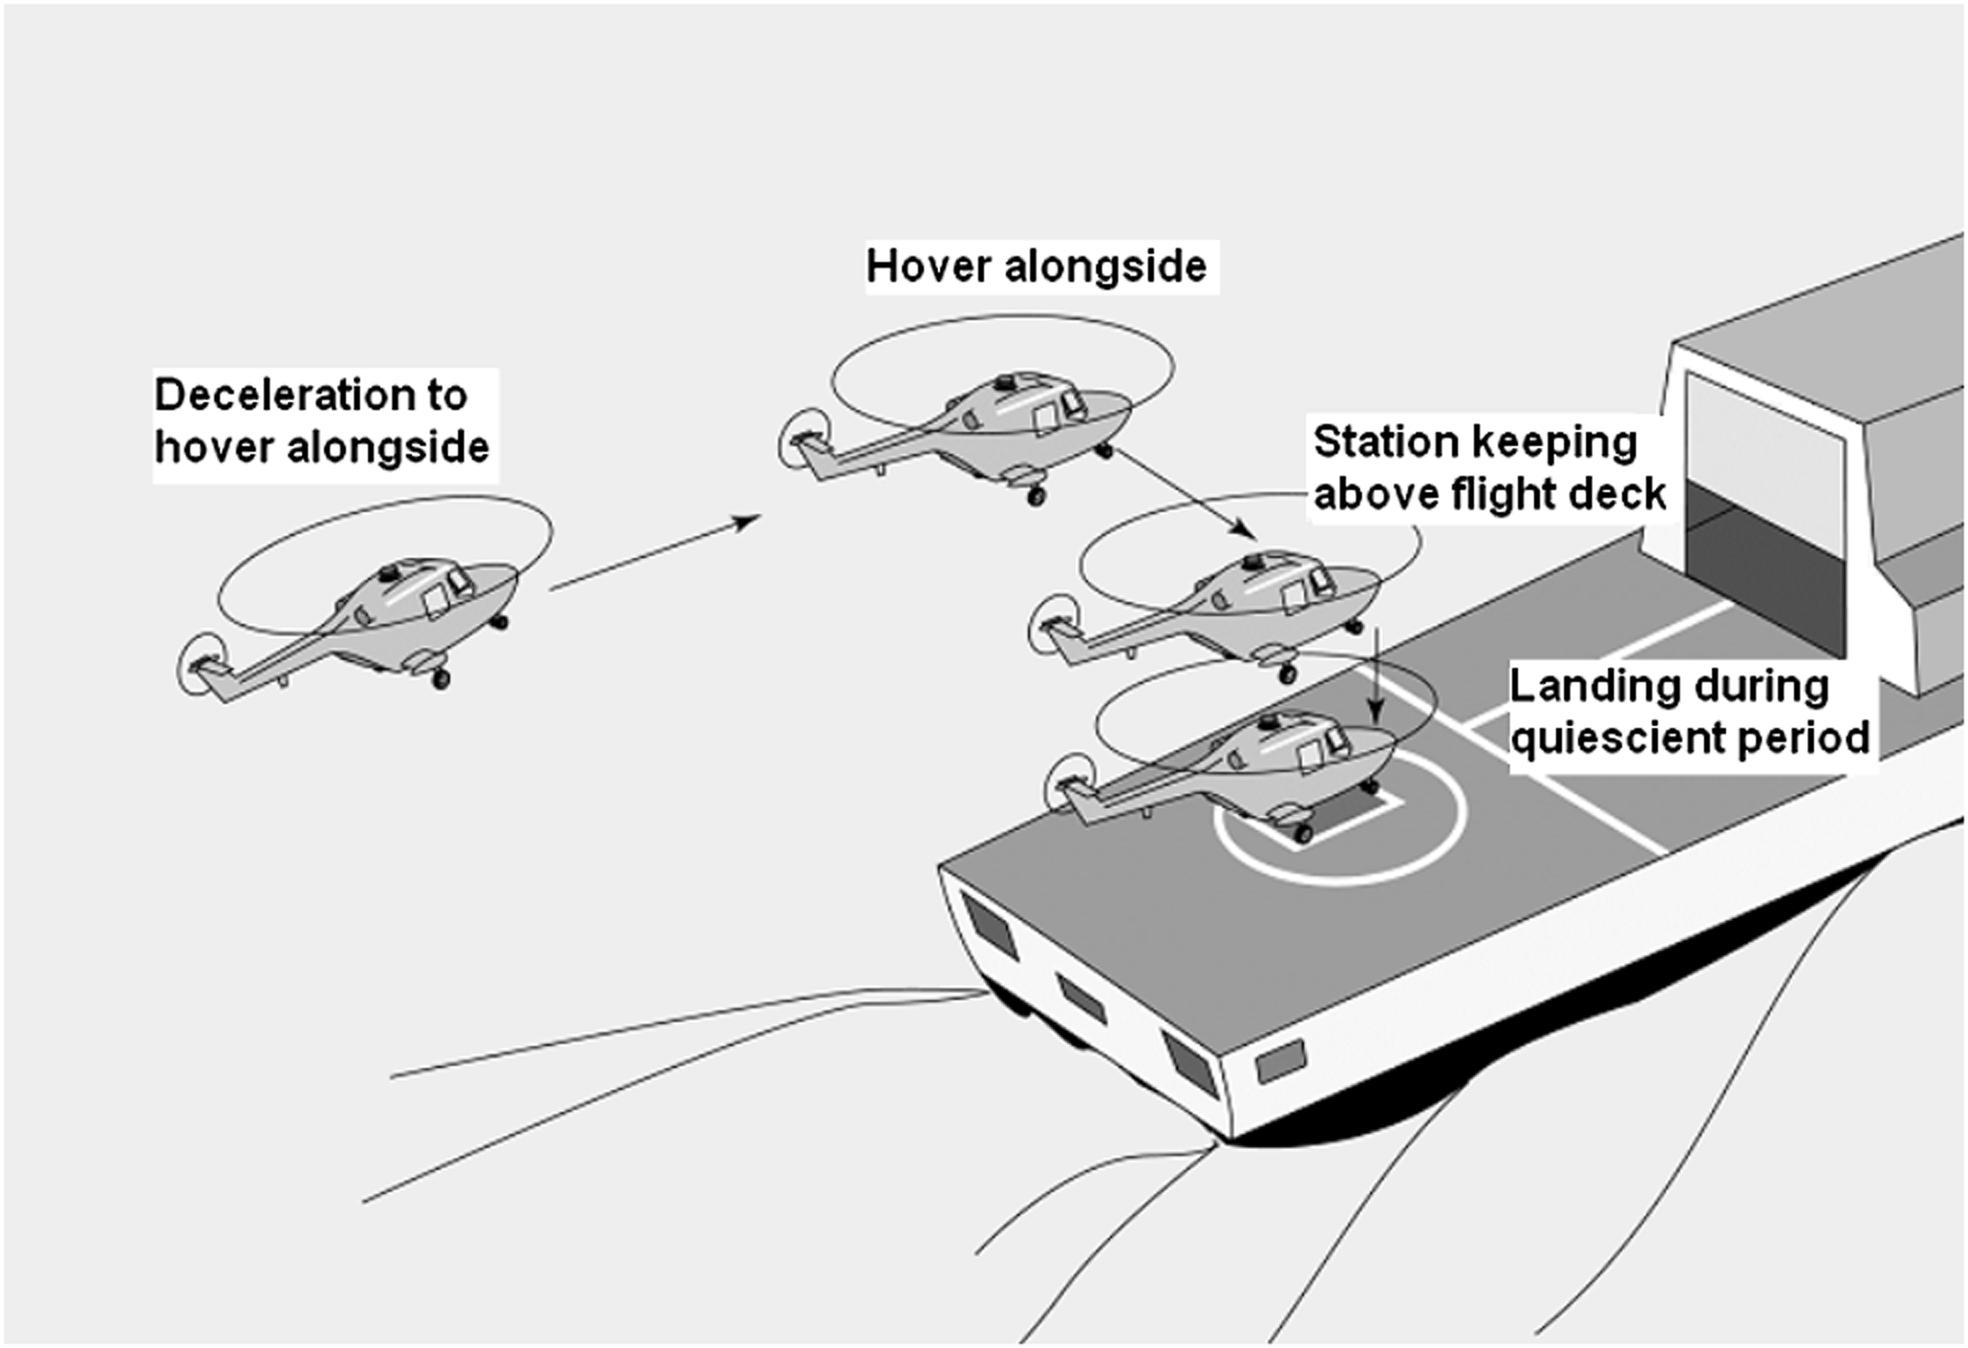
\includegraphics[width=1\textwidth,height=0.3\textheight,keepaspectratio]{figures/landing}
\par\end{centering}
\caption{\label{fig:landing}英国海军舰载直升机着舰标准作业流程\upcite{K_ri__2012}}
\end{figure}


\section{国内外研究现状}

旋翼是直升机最主要的气动部件,其对流场的周期性扰动使得直升机外流场具有显著不同于定翼机外流场的特征。因此,旋翼空气动力学构成了直升机空气动力学的主体(后者还包括旋翼与机身、地面的气动干扰),从而也构成了舰载直升机空气动力学(侧重于研究旋翼尾迹与海面气流、船体气流尾迹之间的气动干扰)的基础。旋翼空气动力学的研究方法包括试验和计算两大类,前者可分为定性试验与定量试验,后者包括基于拉格朗日观点的涡方法、基于欧拉观点的“计算流体动力学
(computational fluid dynamics, CFD\nomenclature{CFD}{computational fluid dynamics})”方法以及兼具二者优势的混合方法。

舰载直升机所特有的空气动力学问题,主要表现为海面自由来流和船舶气流尾迹与旋翼尾迹的相互作用。起飞和着舰过程中,海面和舰面阻挡旋翼尾迹向下游移动,引起的“地”面效应,也是影响直升机飞行安全的重要因素。研究海面、舰面与旋翼之间的气动干扰,是舰载直升机舰面空气动力学的主要任务。与旋翼空气动力学类似,该领域的研究方法也分为试验和计算两大类。

\subsection{旋翼空气动力学试验}

对旋翼流场的试验研究始终伴随和促进着旋翼飞行器的发展,拓展着人们对旋翼空气动力学理解的深度和广度,不断为物理模型和计算方法的验证提供新的数据支持。得益于试验技术的不断进步,对旋翼空气动力学的试验研究经历了从定性到定量,从总体力学参数测量到高分辨率流动细节捕捉的发展过程。

\subsubsection{定性试验}

最简单的旋翼空气动力学“试验”并不需要经过人为的设计,也不需要使用任何试验设备。当空气的温度、湿度、气压满足一定的条件时,旋翼桨尖涡周围会出现自然凝结现象(如图
\ref{fig:natural-condensation} 所示),从而很容易让人们观察到桨尖涡的存在。基于这种观察,人们对旋翼流场有了最基本和最直观的理性认识,发现了旋翼尾迹由桨尖涡主导、尾迹收缩等重要物理事实。
\begin{figure}[h!]
\begin{centering}
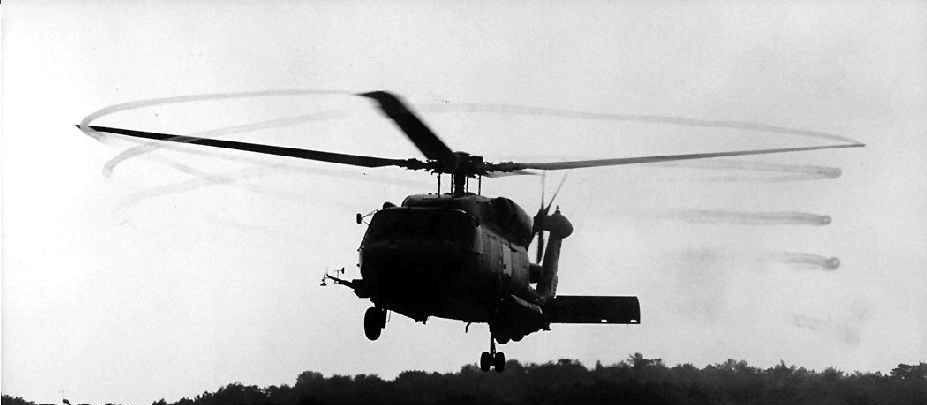
\includegraphics[width=1\textwidth]{../review/figures/natural-condensation}
\par\end{centering}
\caption{\label{fig:natural-condensation}通过自然凝结现象观察到的旋翼桨尖涡\upcite{Leishman1998}}
\end{figure}

为了在不具备自然凝结条件的时候也能对旋翼尾迹进行观察,喷烟法被引入旋翼空气动力学的研究中。1951年,Drees 等\upcite{Drees1951}利用这种方法开展了旋翼流场的流动显示试验。该试验通过在风洞引入喷烟装置,获得了直升机在悬停、前飞、下降等状态下旋翼附近的流动图像,并重点研究了旋翼处于“涡环状态
(vortex ring state, VRS)”时的流动图像。

桨尖涡涡核区与背景流场的空气密度的差别,对折射率等光学特性有显著影响。基于该原理和频闪摄影技术,人们发明了纹影法和阴影法,并将其引入旋翼空气动力学的研究中。1993年,Bagai
\& Leishman\upcite{Bagai1993}利用该方法研究了螺旋桨和旋翼桨尖涡的几何结构,观察到了旋翼尾迹的不稳定(非周期)现象。

定性试验虽然没有给出描述流场的各物理量的具体数值,但给出了各种飞行状态下的旋翼尾迹结构的物理图像,并初步验证了一些早期旋翼空气动力学理论(如滑流理论)的结论。随着测量技术的进步,一些定性试验方法后来发展成为定量试验方法,或发展成为定量试验的一个前置环节。

\subsubsection{定量试验}

根据所测量的物理量以及对流场刻画的精细程度,可以将旋翼空气动力学定量试验大致分为两大类:
\begin{description}[wide]
\item [{测力试验}] 主要用于反映气流对旋翼影响的宏观效果。利用六分量天平、扭矩天平等仪器设备,可以对旋翼中心或全机参考点处的三个力分量和三个力矩分量进行测量。由于试验原理和试验设备都比较简单,所得的试验数据经过简单处理即可应用于结构动力学和飞行动力学分析,因此这类试验至今仍受到许多研究机构的重视。
\item [{测速试验}] 主要用于研究流场的流动细节。根据测量对象的范围,测速试验又可分为单点测量和多点测量两类。早期的单点测量试验主要采用“热线测速仪
(hot wire anemometer, HWA\nomenclature{HWA}{hot wire anemometer})”等介入式测量设备,测速探头本身对流场会造成一定干扰,因此测量结果不能完全反映真实流动情况。这一弊端后来被“激光多普勒测速
(laser doppler velocimetry, LDV\nomenclature{LDV}{laser doppler velocimetry})”技术所克服,但
LDV 仍属于单点测量技术。同属于非介入式测量技术的“粒子成像测速 (particle image velocimetry, PIV\nomenclature{PIV}{particle image velocimetry})”技术,解决了多点同步测量的难题,能够实现对流场(流速)的高分辨率测量,目前已成为流体力学新发现的重要来源,也是验证数值计算方法的重要依据。
\end{description}

1983 年, Sun \& Curtiss\upcite{Sun1983,Sun1989} 利用 HWA 定量测量了模型旋翼的诱导速度分布,研究了直升机低空低速飞行时地面效应对其气动性能的影响。结果显示:直升机低空低速飞行时,自由来流和地面将使旋翼尾迹向上卷起,从而显著影响旋翼气动载荷特性;当卷起的尾迹接近桨盘平面并处于旋翼下方时,桨盘前侧诱导速度分布将发生较大幅度的不规则变化,从而引起旋翼气动力和气动力矩的不规则剧烈变化。

1996–1998年,Leishman 等\upcite{Leishman1996,Leishman1998a}利用 LDV 对桨尖涡切向和轴向速度、环量、黏性引起的涡核增大进行了测量,研究了旋翼尾迹的三维速度场;对桨尖涡涡核位置(如图
\ref{fig:tip-vortex-core} 所示)进行了测量,研究了悬停状态桨尖涡的非周期现象。
\begin{figure}[h!]
\begin{centering}
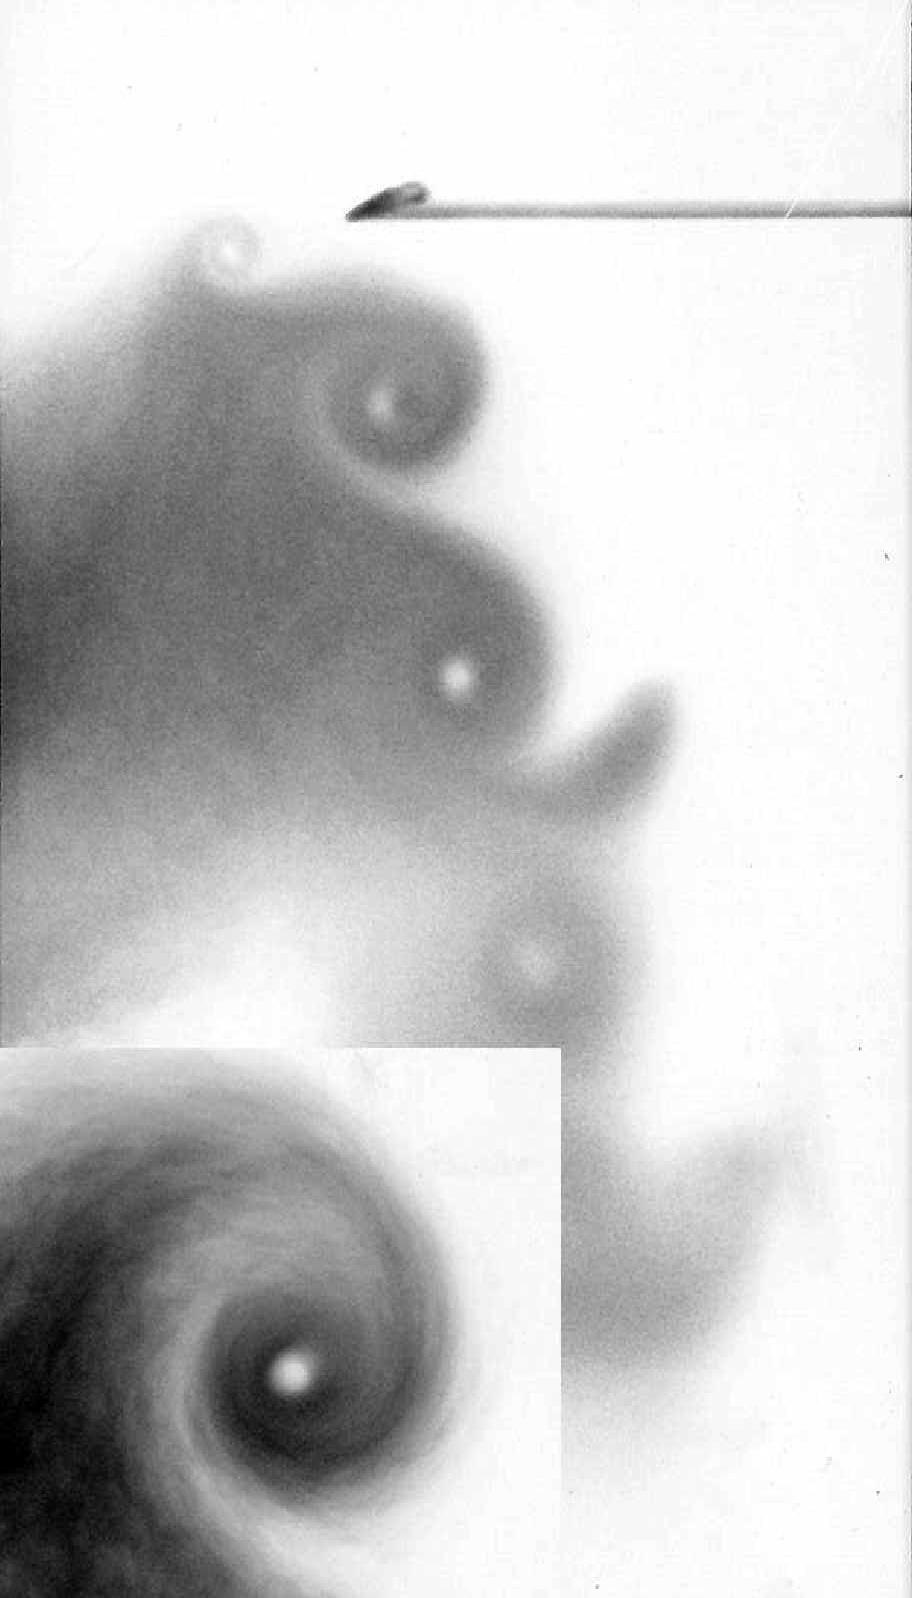
\includegraphics[height=0.26\textheight]{../review/figures/tip-vortex}
\par\end{centering}
\caption{\label{fig:tip-vortex-core}利用喷烟法观察到的旋翼桨尖涡\upcite{Leishman1998}}
\end{figure}

同一时期,南京航空航天大学的唐正飞、高正等\upcite{Tang1997,Tang1998}利用三维 LDV 测量了共轴式双旋翼悬停状态的流场;为了对比,他们对单旋翼流场也进行了测量。测量的物理量包括诱导速度沿三个方向(轴向、径向和周向)的分量,得到了两副旋翼的尾迹相互交汇、干扰的流动图像。

2007年,北京航空航天大学的邓彦敏等\upcite{Yu2007,Ma2012}利用二维 PIV 技术,在水洞中对共轴式双旋翼悬停及不同前飞速度下的流场进行了测量,并对上下两副旋翼的气动干扰特性做了定量研究。该试验测量了流场的瞬时涡量和速度分布、桨尖涡结构和脱落轨迹、尾迹边界等。结果显示:共轴双旋翼悬停流场由上旋翼所主导;与单旋翼相比,双旋翼的尾迹结构更加不稳定。

以上定量试验结果,为旋翼气动设计提供了重要参考信息,也为验证分析模型和计算方法提供了参照对象。

\subsubsection{试验小结}

试验研究表明,旋翼流场具有以下关键特征\upcite{Leishman2006,Johnson2013}: 
\begin{description}[wide]
\item [{桨尖涡主导}] 虽然流体力学界对于“涡 (vortex)”的定义仍存在分歧\upcite{Tong2009}, 但是无论根据何种定义,从试验事实中总能一致地识别出旋翼桨尖涡的存在。试验观测和数值计算都显示,旋翼高速旋转时,每片桨叶的桨尖和桨根处会各拖出一条集中涡。其中,桨根涡自生成后会迅速耗散并失去规则的涡结构,而桨尖涡自生成后则能在较长时间内保持强度和涡结构,因而主导着旋翼流场。定量研究进一步表明,桨尖涡的涡核半径很小,涡核内速度梯度较大,涡核外则接近无旋流动。这一流动特征对试验观测和数值计算在分辨率的空间配置上提出了不同的需求。 
\item [{非定常}] 桨叶的固体表面对于空气流场而言,属于移动的固壁边界。通常,桨叶绕旋翼轴作周期运动时,描述其周围流场的各物理量的也随时间近似按周期变化。即使是悬停状态,虽然桨叶附近的空气流动接近定常状态,但是远离桨盘的桨尖涡也会因系统不稳定而表现出空间和时间的随机性。因此,非定常性是旋翼流场固有的特征,这决定了与旋翼相关的流动问题的研究难度往往要高于固定翼所对应的问题。 
\item [{动态失速}] 通过简单的运动学分析可知,直升机处于前飞状态时,后行侧桨叶剖面的迎角大于前行侧,容易发生失速。另一方面,桨叶剖面的迎角随旋翼转动而周期变化,这种迎角的周期变化会导致翼型气动力出现时滞效应。
这种动态失速现象,使得许多对固定翼行之有效的定常或准定常分析方法对旋翼不再适用。
\item [{局部可压缩}] 直升机旋翼桨尖速度的设计值属于高亚声速范围,压缩性已较为明显。随着前飞速度增大,在前行侧桨叶桨尖处可能会出现局部跨声速区,甚至产生激波。桨叶的旋转又使得可压缩区域与低速不可压缩区域之间没有固定的、显著的界线。这一流动特征使得原本在固定翼空气动力学中已经形成的分别适用于不可压缩和可压缩流动的分析方法,需经过特殊处理才能应用于旋翼空气动力学的研究。 
\end{description}

上述旋翼流场所固有的流动特征,使得旋翼空气动力学的研究难度明显大于固定翼空气动力学。除此之外,以下在直升机各种常见工作状态中普遍存在的气动干扰现象(如图
\ref{fig:helicopter-aerodynamic-interference} 所示)也增加了问题的复杂程度。
\begin{figure}[h!]
\centering{}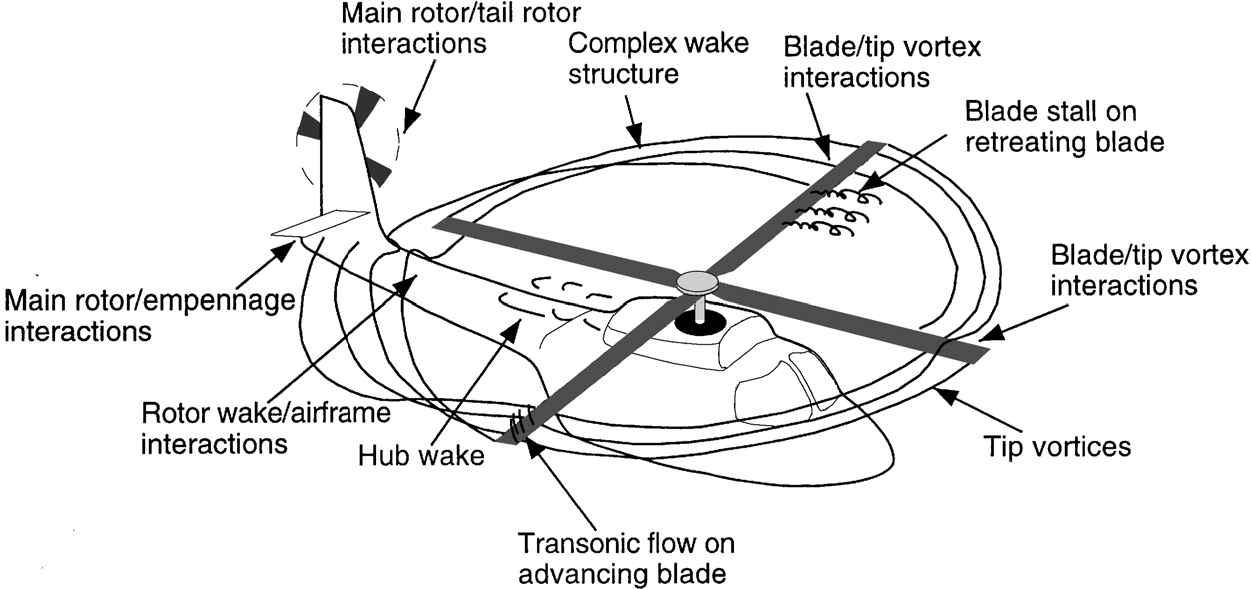
\includegraphics[width=1\textwidth,height=0.22\textheight,keepaspectratio]{../review/figures/aero-interaction}
\caption{\label{fig:helicopter-aerodynamic-interference}直升机气动干扰示意图\upcite{Leishman1998}}
\end{figure}

\begin{description}[wide]
\item [{桨–涡干扰}] 在下降、俯冲、大机动等飞行条件下,或对于桨盘面积有重叠的双旋翼构型,桨尖涡与桨叶之间不可避免地会发生碰撞。桨尖涡经过桨叶时,桨叶表面的压力分布受到强烈扰动,从而成为旋翼振动和噪声的重要来源。
\item [{旋翼–机身干扰}] 通常,直升机机身处于旋翼的下游区域,对旋翼尾迹起阻挡作用。旋翼拉力、悬停气动效率这些重要的总体性能指标将受到影响。另一方面,桨尖涡以一定频率与机身发生碰撞,使得机身表明的压力分布受到扰动,从而成为机体振动的重要来源。 
\item [{旋翼–固定翼干扰}] 直升机上除了旋翼以外,一般还有水平尾翼、垂直尾翼等固定翼面,用于增加飞行稳定性,或提供额外的操纵面。当这些固定翼面受到旋翼尾迹扰动时,其上感知的气动力有别于相应孤立部件在相同自由来流条件下所感知的气动力,从而会影响全机的配平和稳定性。
\item [{旋翼–地面干扰}] 当直升机从地面起飞或贴地低空飞行时,地面的阻挡将改变旋翼尾迹的流向。一般而言,地面效应会使旋翼拉力、悬停气动效率等总体性能指标有所提升;但在地面存在大量砂石等颗粒物的条件下,地面效应会进一步引发沙盲现象,导致飞行员视线受到遮挡,从而影响飞行安全。 
\end{description}

以上旋翼流场特有的关键特征和直升机特有的气动干扰现象,始终是旋翼空气动力学研究的关键问题。许多在固定翼空气动力学中得到成功应用的方法,在应用到旋翼空气动力学研究之前,必须经过适当的改造;旋翼空气动力学本身也产生了一些特有的分析模型和数值计算方法,并且还在不断发展和改进。

\subsection{旋翼空气动力学计算}

\subsubsection{入流模型}

入流模型描述的是旋翼尾迹在桨盘平面处的诱导速度与旋翼气动力之间的函数关系,其发展历程经历了滑流理论、动态入流和有限状态入流三个阶段。

滑流理论,又称动量理论,是最早也是最简单的入流模型。该理论基于作用盘模型和动量定理,给出的悬停状态下桨盘平面的诱导速度为\upcite{Johnson1994}:
\begin{equation}
v_{\mathrm{0}}=\sqrt{\frac{C_{T}}{2}}
\end{equation}
其中,$C_{T}$ 是旋翼拉力系数,$v_{\mathrm{0}}$ 是无量纲诱导速度。该模型只给出了沿桨盘平面均匀分布的诱导速度场,并且属于静态(准定常)入流模型,所以通常只在初步设计阶段被用来进行旋翼性能估算。此后,各种改进的静态入流模型不断被提出,桨盘平面诱导速度分布的非均匀性得以体现。

在此基础上,出现了一阶状态空间方程形式的动态入流模型,以考虑旋翼气动力与入流关系的非定常性,其中最具代表性的是 Pitt–Peters
动态入流模型。在该模型中,桨盘上任意一点的无量纲诱导速度 $v$ 可以写为无量纲展向位置 $r$ 和气流方位角 $\psi$
的函数:
\begin{equation}
v=v_{0}+v_{\mathrm{c}}r\cos\psi+v_{\mathrm{s}}r\sin\psi,
\end{equation}
其中 $v_{\mathrm{0}},v_{\mathrm{s}},v_{\mathrm{c}}$ 分别为均匀入流分量、横向入流分量、纵向入流分量。这三个无量纲诱导速度分量和它们的无量纲时间导数,与桨盘的三个无量纲气动力
$C_{T},C_{L},C_{M}$ 之间的关系,被写成状态空间形式:
\begin{equation}
\left(\underline{M}\,\dv{t}+\underline{L}^{-1}\right)\begin{bmatrix}v_{\mathrm{0}}\\
v_{\mathrm{s}}\\
v_{\mathrm{c}}
\end{bmatrix}=\begin{bmatrix}C_{T}\\
C_{L}\\
C_{M}
\end{bmatrix}
\end{equation}
文献 \cite{Chen1989} 对截至 1980 年代末的各种静态、动态入流模型做了详细的综述。

1989年,He\upcite{He1989,Peters1995} 基于势流理论,提出了广义动态尾迹模型,又称 Peters–He
有限状态入流模型。该模型将状态变量个数推广到任意多,进一步体现了高阶谐波的影响。值得注意的是,经典的动量理论模型是 Pitt–Peters
动态入流模型在准静态情况下的特例,Pitt–Peters 动态入流模型又是 Peters–He 有限状态入流模型只取一阶状态变量时的特例。

动态入流模型具有形式紧凑、计算效率高的优点,在直升机飞行动力学建模\upcite{Yang1996,Sun2001}和旋翼气动弹性问题\upcite{Panda1985,Jang1988}的研究中得到了广泛的应用。

但是,以上所有入流模型都是从作用盘模型出发,引入尾迹形状规则且无限延伸等理想化假设,最后得到气动力与入流系数的关系。显然,这种简单的物理模型无法真实反映旋翼流场由桨尖涡主导、局部可压缩等特性,也无法处理存在复杂气动干扰的问题,已经逐步被更接近物理真实的自由尾迹模型取代。

\subsubsection{尾迹模型}

尾迹模型是用于描述旋翼尾迹中涡量空间分布情况的物理模型,在一些文献中也用来指代该物理模型所对应的数值计算方法。该模型的基本思想是用直线或曲线涡元(涡线单元)对涡量场进行离散,通过研究涡线单元的运动和演化来描述涡量场,属于连续介质力学\upcite{Fung1994}中的拉格朗日观点(质点系观点)。得到涡量场后,再利用
Biot–Savart 定律对涡量场进行积分,从而得到诱导速度场。从发展历程来看,尾迹模型经历了刚性尾迹,预定尾迹和自由尾迹三个阶段。

\paragraph{刚性尾迹模型}

刚性尾迹模型假设旋翼尾迹中的涡量集中分布在以桨盘为底面的直圆柱面或斜圆柱面上,或集中分布在从桨尖拖出的螺旋线上。在此模型中,涡系的几何形状只受自由来流和平均入流的驱动,不因涡系自诱导和互诱导而发生变形,故而得名“刚性
(rigid)”尾迹。

由于刚性尾迹的几何形状简单,经过一些数学推导,有时可以得出初等函数、特殊函数或级数形式的解。2004 年,北京航空航天大学的陈铭\upcite{Chen2003,Chen2004,Chen2005}利用刚性尾迹模型,将旋翼用作用盘代替,对共轴双旋翼前飞气动特性进行了研究,得到了解析形式的诱导速度解。

虽然根据刚性尾迹模型得出的解析形式的解能够快速给出计算结果,但其所假设的尾迹几何结构与实际情况相差较大。尤其是在大机动、贴地飞行等条件下,尾迹畸变严重,刚性尾迹模型不再适用。目前,刚性尾迹模型只被用于对实时性要求极高的飞行仿真程序,或用于为自由尾迹模型、CFD
求解器提供迭代初值。

\paragraph{预定尾迹模型}

预定尾迹模型在刚性尾迹模型的基础上,根据一些特殊旋翼在特殊状态下的试验结果,引入一些参数对刚性尾迹的几何形状进行修正。1971 年,Landgrebe\upcite{Landgrebe1971}基于水洞试验,提出了一种半经验的旋翼尾迹模型。
但该模型的适用性严重依赖于根据个别试验确定的经验参数,普适性较差,并没有从根本上解决刚性尾迹模型无法准确描述尾迹几何结构的问题。

\paragraph{自由尾迹模型}

自由尾迹模型允许涡元像流体微团一样在流场中自由运动。这里的“自由”是指相对于刚性尾迹和预定尾迹,自由尾迹不再对尾迹几何结构进行限制,涡元(流体微团)的运动仍然受流体力学基本原理支配。该模型所依据的“涡元像流体微团一样在流场中自由运动”是指涡元运动满足如下关系:
\begin{equation}
\frac{\dd\vec{r}}{\dd t}=\vec{u}=\vec{u}_{\infty}+\vec{u}_{\mathrm{ind}}\label{eq:vortex_element}
\end{equation}
其中,$\vec{r}$ 是涡元位置,$\vec{u}_{\infty}$ 是自由来流速度,$\vec{u}_{\mathrm{ind}}$
是旋翼涡系对该点的诱导速度。该诱导速度需根据 Biot–Savart定律\upcite{Anderson_2017}计算得到。考虑
$A,B$ 两点之间一段强度为 $\Gamma$ 的涡线,它对空间任意一点 $C$ 的诱导速度由以下积分给出:
\begin{equation}
\vec{u}_{\mathrm{ind}}^{C}=\int_{A}^{B}\frac{\Gamma}{4\pi}\frac{\dd\vec{l}\times\vec{r}}{r^{3}}
\end{equation}
引入涡线模型离散后,式 (\ref{eq:vortex_element}) 变为一个高度非线性的常微分方程组。

式 (\ref{eq:vortex_element}) 所表示的“涡元像流体微团一样在流场中自由运动”,实际上是 Kelvin 定理\footnote{在理想流体中,沿一条封闭物质线的速度环量不随时间变化\upcite{Cottet2000}。}应用到理想流体时的一个推论,因而自由尾迹模型的成立条件是流体无黏、正压且外力有势。在旋翼尾迹问题中,外力(重力)可以忽略,流体(空气)满足正压条件,但黏性通常不可忽略,为此需引入黏性涡核模型\upcite{Leishman2006}进行修正。该模型可进一步分有限涡核模型和涡核演化模型两部分。简单的集中涡线模型存在奇异性,为消除这种奇异性,通常以一个截面半径为有限值的涡管代替截面半径为零的集中涡线。在有限涡核模型的基础上,令涡核半径随涡龄的增长而变大,以此来体现空气黏性引起的涡量耗散,涡核以外的流体则认为是无黏的。

最早尝试利用自由尾迹模型对旋翼流场进行建模的有 Scully\upcite{Scully1967,Scully1975}、Landgrebe\upcite{Landgrebe1969}等。这些早期的自由尾迹算法普遍存在收敛性差的问题,此后一段时间,许多学者在改善该模型的收敛性方面做了大量工作。

1983 年,美国普林斯顿大学的 Sun \& Curtiss\upcite{Sun1983,Sun1989a} 建立了一种简化的自由尾迹卷起模型,用以研究旋翼尾迹与地面的相互影响,并在此基础上计算了桨盘平面的诱导速度分布。结果显示:地面和卷起涡显著地改变了旋翼近尾迹的几何形态,从而造成了桨盘平面诱导速度分布的剧烈变化。

自 1990 年代起,美国马里兰大学的 Leishman 团队提出和改进了多种自由尾迹算法。1993年,Crouse \& Leishman\upcite{Crouse1993}
提出了一种“预估校正 (predictor–corrector, PC)”格式,用于提高收敛性,控制计算量。该算法采用两点中心差分格式对涡量场进行时间和空间离散,并通过引入周期条件确保稳态解收敛。但对悬停状态客观存在的非周期解,无法给出正确的计算结果。1995
年,Bagai \& Leishman\upcite{Bagai1995,Bagai1995a,Bagai1996} 提出了一种“伪隐式预估校正
(pseudo-implicit predictor–corrector, PIPC)”格式,用于求解存在稳态周期解的旋翼尾迹问题。该算法采用五点中心差分格式对涡量场进行时间和空间离散,并利用松弛迭代法和周期条件改善解的收敛性。基于该算法,他们计算了单旋翼、双旋翼构型的直升机在悬停、低速前飞、高速前飞等各种飞行状态中的旋翼尾迹,结果很好地反映了旋翼尾迹的畸变。但该方法用到了周期条件,因而只适用于存在稳态周期解的问题;但也有学者质疑稳态周期解的存在性\upcite{Kini2002}。另外,参数分析表明,解的收敛性和尾迹几何结构与部分经验参数的选取有关,使该方法的通用性受到质疑。2000–2004年,Bhagwat
\& Leishman\upcite{Bhagwat2000,Bhagwat2000a,Leishman2002,Leishman2004}
提出了一种“时间精确”自由尾迹模型,用于分析旋翼尾迹的动态响应过程。该算法采用“二阶后向差分预估校正 (predictor–corrector
2nd-backward, PC2B)”格式,提高了算法的数值稳定性。由松弛迭代法(如 Bagai 的 PIPC 格式)给出初始条件后,可以沿时间积分尾迹方程和桨叶动力学方程,得到旋翼尾迹和桨叶运动的动态响应值。基于该算法,他们计算了多种旋翼构型在不同飞行条件下的尾迹几何形态(如图
\ref{fig:free-wake} 所示),研究了旋翼做机动时的尾迹瞬态变化过程,并对涡环状态这一典型的不稳定状态进行了模拟。该模型在以上算例中均给出了很好的结果。2006年,Gupta
\& Leishman\upcite{Gupta2006} 将上述时间精确自由尾迹模型应用到风力机械的气动性能研究中。同年,Ananthan
\& Leishman\upcite{Ananthan2006} 基于时间精确自由尾迹模型,研究了机动飞行状态下的旋翼尾迹几何形态和涡量分布,初步研究了桨涡干扰引起的旋翼噪声。此后,该校的
Ribera \& Celi\upcite{Ribera2007} 也利用该模型开展了一些直升机飞行动力学方面的研究。
\begin{figure}[h!]
\centering{}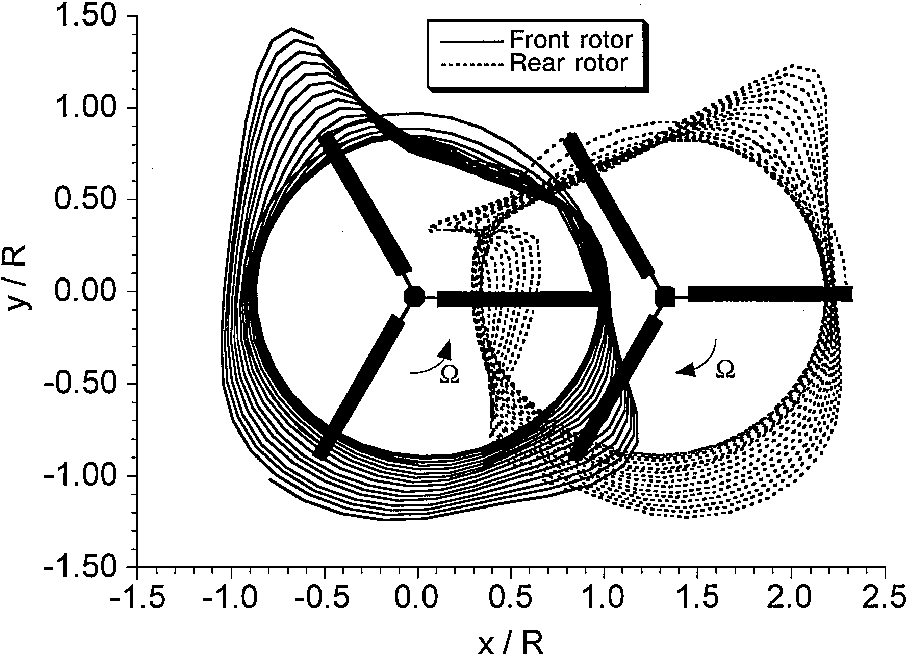
\includegraphics[width=1\textwidth,height=0.26\textheight,keepaspectratio]{../review/figures/free-wake}
\caption{\label{fig:free-wake}利用自由尾迹模型计算得到的纵列式双旋翼尾迹\upcite{Leishman2002}}
\end{figure}

\newpage{}

本世纪初,美国俄亥俄州立大学的 Conlisk 团队\upcite{Conlisk2001}也开展了一些自由尾迹模型算法方面的研究。2000年,Jain
\& Conlisk\upcite{Jain2000} 采用升力线理论对桨叶进行建模,采用时间步进自由涡方法对桨尖涡运动进行计算。在做时间步进积分时,他们采用了数值稳定的四阶隐式
Adams–Moulton 格式。基于上述方法,他们通过数值计算研究了在试验中观察到的两条桨尖涡之间相互缠绕的现象。2002年,Kini
\& Conlisk\upcite{Kini2002} 采用与文献 \cite{Jain2000} 中类似方法研究了悬停状态桨尖涡几何结构的稳定性。计算结果显示,悬停状态时,桨尖涡几何结构的周期性条件只对前几圈桨叶适用,后几圈的桨尖涡几何结构表现出明显的时间非周期性。由于采用了数值稳定的隐式
Adams–Moulton 格式,并且在步长小于 $\ang{4}$ 时可以给出足够精确的结果。此文认为,物理不稳定是导致悬停状态桨尖涡远场尾迹非周期结构的主要原因,而非算法的数值稳定性问题。这与
Leishman 团队的观点\upcite{Bagai1995,Bagai1995a,Bagai1996}相反。2006年,Pulla
\& Conlisk\upcite{Pulla2006} 基于时间步进自由尾迹方法研究了地面效应影响下的直升机气动特性。其中,旋翼尾迹通过自由涡方法进行建模,桨叶气动力由升力面理论给出,地面则采用镜像法进行处理。时间步进算法采用与文献 \cite{Jain2000,Kini2002}
中类似的 Adams–Moulton 格式。计算结果与佐治亚理工的试验数据进行了对比,验证了算法的可行性。

在国内,自由尾迹模型也有相应的发展和应用。2007 年,南京航空航天大学的李春华、徐国华等\upcite{Li2007}基于时间精确自由尾迹模型,研究了倾转旋翼的气动特性;2010
年,该校的李攀、陈仁良等\upcite{Li2010} 基于时间精确自由尾迹模型,提出了一种新的差分格式,建立了一种高置信度的直升机飞行动力学模型。2014
年,北京航空航天大学的陈铭等\upcite{Wang2014}基于稳态自由尾迹模型,研究了旋翼几何参数对共轴双旋翼悬停性能的影响;2015
年,该校的曹义华等\upcite{Lv2015}采用自由尾迹模型和面元法,分别对旋翼和机身进行建模,建立了一种旋翼–机身气动干扰模型,并进行了配平计算。

尽管自由尾迹模型仍然是目前直升机工程界普遍认可的旋翼空气动力学分析手段,但该模型本身也存在一定的局限性。首先,自由尾迹模型必须与其他模型(如升力面模型)配合,才能获得桨尖涡环量的初始值。其次,目前常用的涡核模型都存在若干经验参数,并且桨尖涡的截断位置也需要人工设置。另外,这种物理模型虽然能够大体上还原桨尖涡的几何结构,但在处理桨尖涡与固体壁面碰撞等问题时,只能采取回避或镜像处理的方法,无法描述涡结构破碎等现象。

\subsubsection{黏性涡粒子模型\label{sec:Viscous-Vortex-Particle-Method}}

“黏性涡粒子模型/方法 (vortex particle model/method, VPM\nomenclature{VPM}{vortex particle model/method})”与自由尾迹模型类似,也属于基于拉格朗日观点的分析模型。不同的是该模型用涡粒子代替了涡线,每个涡粒子由位置
$\vec{r}$ 和涡量 $\vec{\omega}$ 两个矢量来描述。其中,涡元位置的变化规律与自由尾迹模型一样,由如下简单的运动学关系描述:
\begin{equation}
\frac{\dd\vec{r}}{\dd t}=\vec{u},
\end{equation}
而涡量的变化规律则由涡量输运方程给出。旋翼尾迹流场属于低亚声速流动,通常可以对空气采用各项同性、不可压缩、正压等理想化假设。基于这些假设,可以将
Navier–Stokes 方程(详见 \ref{sec:Navier-Stokes-Equation} 小节)简化为: 
\begin{equation}
\frac{\partial\vec{u}}{\partial t}+\left(\vec{u}\cdot\nabla\right)\vec{u}=-\frac{1}{\rho}\nabla p+\nu\nabla^{2}\vec{u}+\vec{f}
\end{equation}
利用矢量分析公式\upcite{Zorich2004}、涡量定义\footnote{$\vec{\omega}=\nabla\times\vec{u}$}、不可压\footnote{$\nabla\cdot\vec{u}=0$}、正压\footnote{$\nabla\rho\times\nabla p=\vec{0}$}、体积力有势\footnote{$\vec{f}=-\nabla V$}等条件,可将上式改写成涡量形式:
\begin{equation}
\frac{\partial\vec{\omega}}{\partial t}+\left(\vec{u}\cdot\nabla\right)\vec{\omega}=\vec{\omega}\cdot\nabla\vec{u}+\nu\nabla^{2}\vec{\omega}\label{Vorticity-Transport-Equation}
\end{equation}
该式左端为涡元涡量的物质导数,右端第一项表示涡元变形(拉伸、弯曲)的影响,右端第二项表示黏性引起的涡量扩散。 此即不可压缩、正压流体的涡量输运方程。

2009年,He 等\upcite{He2009}利用 VPM 研究了旋翼尾迹中涡量的输运和扩散现象。该方法避免了基于欧拉观点的数值离散方法所引入的数值耗散。计算结果显示:VPM
可以精确模拟旋翼尾迹在悬停、前飞等状态下的动态变化;不借助经验参数,很好地捕捉到了尾迹收缩、桨尖涡卷起、涡量扩散等物理现象;尾迹对总距突增操纵的动态响应计算结果与试验吻合很好。此文中的旋翼尾迹初始涡量由升力线模型获得。此文指出了用
CFD 替代该模型的可能性,但没有进一步给出具体实施方法和计算结果。

2012年,南京航空航天大学的魏鹏、徐国华等\upcite{Wei2012,Wei2012a}基于VPM建立了一种适用于旋翼非定常流场特性分析的数值方法。桨叶附着涡以及新生涡环量由升力面模型\upcite{Weissinger1947}给出。计算结果显示:该方法与自由尾迹模型和CFD相比,能够在兼顾效率的同时,更好地捕捉旋翼尾迹运动(如图
\ref{fig:vortex-particle} 所示)。但升力面模型只适用于势流,并不能很好反映动态失速、桨尖激波等现象。
\begin{figure}[h!]
\centering{}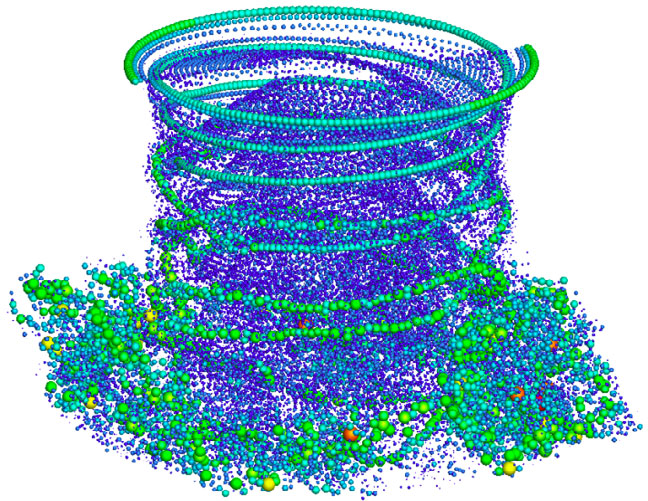
\includegraphics[height=0.26\textheight]{../review/figures/vortex-particle}
\caption{\label{fig:vortex-particle}利用黏性涡方法计算得到的涡元分布\upcite{Wei2012}}
\end{figure}

2014年,清华大学的王浩文等\upcite{Tan2014}采用非定常面元法、VPM 及涡量镜面法,建立了旋翼–平尾非定常气动干扰分析模型。计算结果显示,此方法计算精度高于时间精确自由尾迹,计算效率高于
CFD。但面元法只适用于势流,并不能真实反映桨叶表面的分离、压缩性等流动现象。

从上述研究内容来看,VPM 本身可以比较高效(与 CFD 相比)且精确(与自由尾迹相比)地捕捉旋翼尾迹中的典型流动现象;但在处理桨叶、机身、固定翼面等壁面时,需引入其他模型作为补充。除上面提到的只适用于势流的升力线模型、升力面模型、面元法外,也有研究人员尝试采用
CFD 对近壁面进行处理。

\subsubsection{涡量输运方程\label{sec:Vorticity-Transport-Model}}

该方法基于欧拉观点(场观点),直接对涡量输运方程 (\ref{Vorticity-Transport-Equation}) 进行数值求解。从离散方法的角度看,该方法属于有限体积法,但描述流场的变量为涡量。由于采用了涡量形式的问题表述形式,该方法能够有效地减小数值耗散引起的涡量非物理扩散。涡量输运方法的主要弊端是难以处理壁面边界条件,无法考虑空气压缩性,因而必须引入其他方法(升力线、升力面、CFD
等)作为补充。

2000年,Brown\upcite{Brown2000} 通过求解涡量输运方程,计算了孤立旋翼和共轴双旋翼周围的非定常气动环境,并与试验数据进行了对比验证。由于涡量输运方程不能直接处理壁面边界条件,此文利用升力线方法给出尾迹初始涡量。

2003年,Houston \& Brown\upcite{Brown2000a,Houston2003} 采用有限状态入流模型与涡量输运模型两种方法,研究了直升机配平、自转下滑状等飞行力学问题。计算结果表明,当自转下滑率较小时,两种模型给出的计算结果差别不大;随着下滑角的增大,两者的差别变得明显。同年,Whitehouse
\& Brown\upcite{Whitehouse2003} 将涡量输运方法应用到大型固定翼飞机尾涡与直升机尾迹气动干扰问题的研究中。计算结果显示,直升机高速飞行时,飞机尾涡不会对其造成严重影响;但在低速飞行时,飞机尾涡会引起旋翼气动载荷和气弹响应的振荡,从而增加飞行员操纵的难度。

2005年,Brown \& Line\upcite{Brown2005} 对涡量输运方法进行了改进,使其计算效率得到提高,计算结果如图
\ref{fig:VTM} 所示。新算法引入了一种半拉格朗日自适应网格系统,在尽可能避免产生额外计算量的前提下,显著提高了计算结果的空间分辨率。同时,该网格系统避免了在处理计算区域边界附近尾迹截断时需借助数值边界条件的问题。对于壁面边界条件,此文仍借助升力线模型进行处理。
\begin{figure}[h!]
\centering{}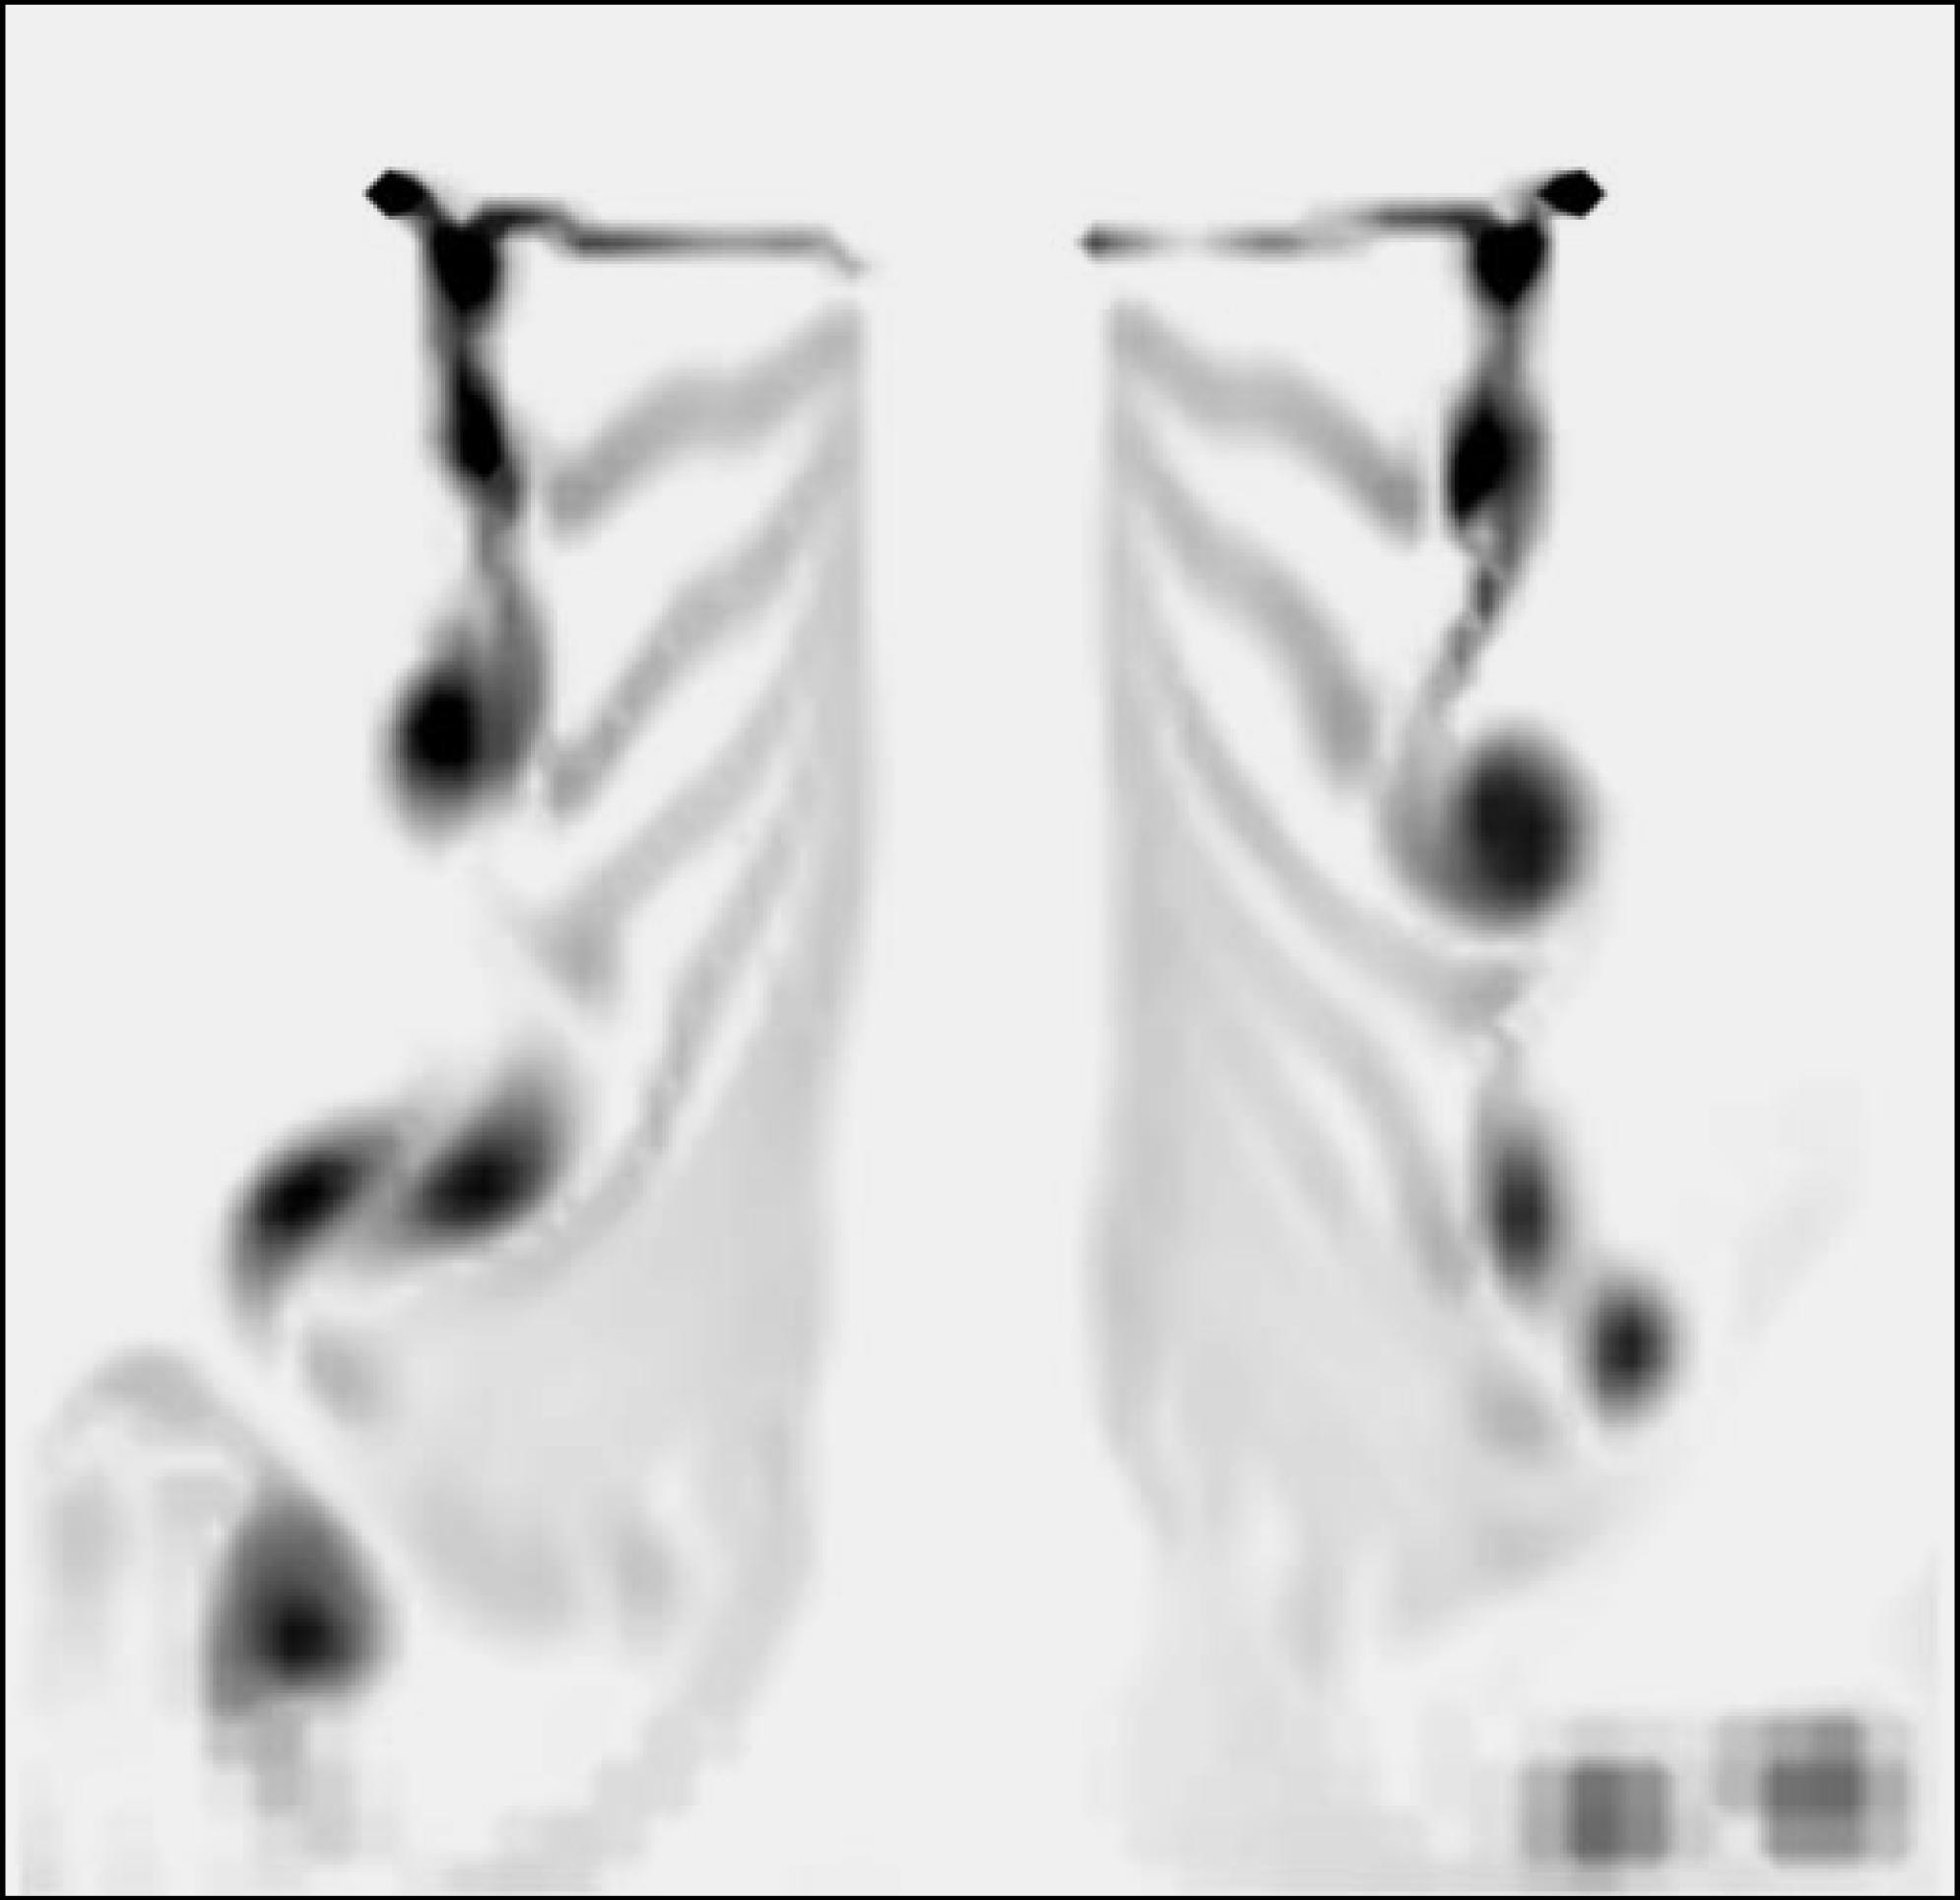
\includegraphics[width=1\textwidth,height=0.26\textheight,keepaspectratio]{../review/figures/vtm}
\caption{\label{fig:VTM}由涡量输运方法计算得到的涡量分布\upcite{Brown2005}}
\end{figure}


\subsubsection{Navier–Stokes 方程\label{sec:Navier-Stokes-Equation}}

Navier–Stokes 方程\upcite{Landau_1987}是连续介质假设下,描述流体运动最精确的物理模型。对此方程的数值求解,构成了
CFD 研究的主流,所涉及的文献浩如烟海,这里只介绍其中与旋翼相关的部分研究内容。

早期的旋翼 CFD 研究完全不考虑空气黏性的影响,因此实际上是在求解 Navier–Stokes 方程的简化版本 —— Euler
方程。1985年,Roberts 等\upcite{Roberts1985}将旋翼流场分为两部分:远离桨叶的部分通过自由尾迹模型给出涡量分布,并计算出响应的诱导速度;靠近桨叶的部分由三维欧拉方程进行描述,利用有限体积法进行求解。基于这种耦合算法,他们研究了孤立机翼和悬停状态的旋翼桨叶附近的流场。1999
年,北京航空航天大学的曹义华等\upcite{Cao1998,Cao1999}也开展了类似的工作。由于没有考虑空气黏性,这种计算模型并不能用于分析旋翼气动效率。

1997 年,北京航空航天大学的康宁、孙茂\upcite{Kang1997} 基于三维定常不可压缩 Navier–Stokes 方程,研究了旋翼受地面效应影响的流动情况。
该方法以时间平均动量源模型\upcite{Rajagopalan1991,Rajagopalan1991a}来体现旋翼对流场的扰动,计算并分析了尾迹畸变、地面涡的形成、桨盘平面诱导速度分布、不同旋翼离地高度及前进比下的地面效应。通过将计算得到的流动图像和旋翼诱导速度与试验值进行对比,验证了算法的适用性。2000
年,他们又将该方法用于分析共轴式和纵列式两种双旋翼构型的地面效应问题研究中\upcite{Kang2000}。该方法对于远离桨叶的流场能够以较小的计算量给出合理的计算结果,但对桨叶表面的流动情况无法给出详细的信息。

2007年,Whitehouse 等\upcite{Whitehouse2007}将涡量输运方程与 Navier–Stokes 方程相结合,建立了一种更加接近物理真实的旋翼空气动力学分析模型。该模型(如图
\ref{fig:VTM-NSE} 所示)采用基于原始变量(速度、压力)的 Navier–Stokes 方程对桨叶附近的流动情况进行描述,可以体现这一区域存在的空气黏性、压缩性等势流模型无法很好处理的流动特性;对涡流主导的尾迹部分则采用基于欧拉观点的涡量输运方程进行描述,可以有效降低常规
CFD 造成的涡量非物理扩散。利用该耦合模型,他们给出了一些固定翼、钝体、直升机上的算例,在流动特性捕捉和非定常载荷计算方面都给出了较好的结果。
\begin{figure}[h!]
\centering{}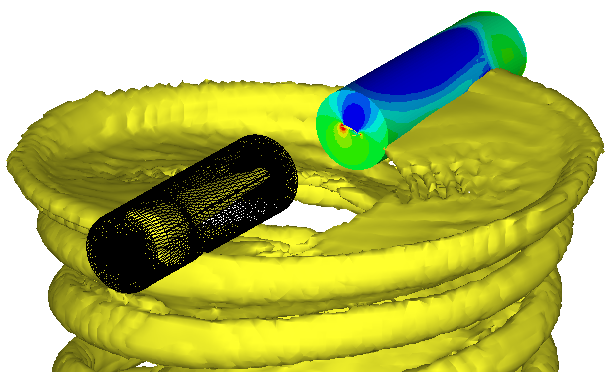
\includegraphics[width=1\textwidth,height=0.26\textheight,keepaspectratio]{../review/figures/whitehouse}
\caption{\label{fig:VTM-NSE}涡量输运方程与 Navier–Stokes 方程耦合模型示意图\upcite{Whitehouse2007}}
\end{figure}

2008年,Anusonti-Inthra 等\upcite{Anusonti-Inthra2008}将 RANS\nomenclature{RANS}{Reynolds-averaged Navier–Stokes}
(Reynolds-averaged Navier–Stokes) 方程与基于粒子的涡量输运方法进行耦合,用于分析固定孤立机翼低速飞行时的气动性能和尾迹特性,并通过与风洞试验数据进行对比,对该计算模型进行了验证。该耦合方法将流场按主要流动特性,分为近壁面和远场区域,分别用三维可压缩
RANS 方程和基于粒子的涡量输运方程进行求解。计算结果显示:该耦合方法可以对机翼翼梢的三维流动效应进行合理的模拟,并且有效解决了常规
CFD 存在的数值耗散问题。但也有学者认为,耦合方法本身及不同计算区域数据交换带来的复杂性,可能会减弱涡粒子模型对计算效率的提升效果\upcite{Kamkar2011}。

\subsubsection{网格自适应加密技术}

对于任何基于离散网格的数值方法而言,加密网格都是提高计算精度的一个重要途径。但是有限的计算资源不允许我们在整个计算区域内无差别地对网格进行加密,而只能有选择地在某些物理量随空间或时间变化剧烈的地方进行加密。另外,加密网格的过程应当尽可能减少对人工操作的需求,且便于逐次递推,这样才能达到充分利用现有计算资源以获得尽可能高的精度的目的。根据上一步基于粗糙网格的计算结果,由计算机自主确定下一步需要对网格进行加密的区域,并通过递推逐次实现网格的精细化,充分利用计算机软硬件资源,以获得尽可能高的计算精度,这就是“自适应网格加密
(adaptive mesh refinement, AMR\nomenclature{AMR}{adaptive mesh refinement})”技术的主要思想。这是解决由涡流主导的旋翼尾迹数值计算问题的关键技术,也是多年以来
CFD 领域的研究热点。

2011年,美国斯坦福大学的 Kamkar \& Jameson\upcite{Kamkar2011,Sankaran2011} 提出了一种适用于涡主导流动问题的自适应网格加密方法。该方法将网格细化过程分为两步:先利用特征检测方法自动识别需要加密网格的区域,再利用基于
Richardson 外插方法的误差估计,给出合适的网格精细程度(分辨率)。此文所用计算网格为“对偶网格 (dual-mesh)”:靠近物体表面用非结构网格处理复杂的几何外形及边界层,远离物体表面的区域用自适应结构网格和高阶格式处理涡流尾迹。结果表明,该方法能够同时提高直升机性能分析精度和尾迹分辨率(如图
\ref{fig:AMR} 所示)。
\begin{figure}[h!]
\centering{}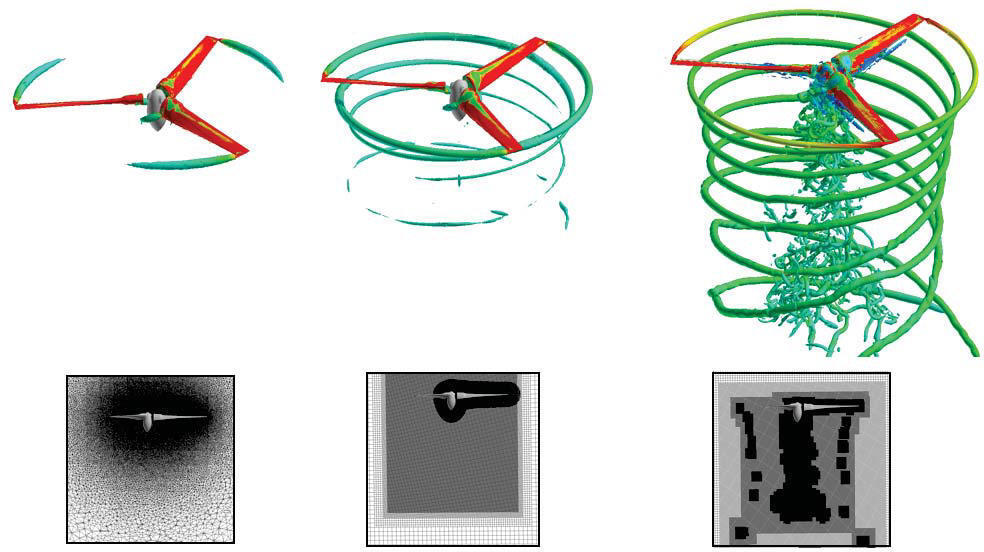
\includegraphics[width=1\textwidth,height=0.24\textheight,keepaspectratio]{../review/figures/adaptive}
\caption{\label{fig:AMR}网格自适应加密对涡量分布计算结果的改善\upcite{Sankaran2011}}
\end{figure}


\subsection{舰载直升机气动干扰试验}

2003 年,Derby \& Yamauchi\upcite{Derby2003} 搭建了一套用于研究直升机与两栖攻击舰气动干扰问题的
$1/48$ 缩比模型。该模型还被用于研究直升机与大型建筑物以及地面的气动干扰问题。此项目对倾转旋翼机、纵列式直升机、单主旋翼直升机三种构型都进行了缩比模型试验,获得的结果可用于指导全尺寸直升机舰上操纵以及编队飞行的研究。

2007 年,Lamar 等\upcite{Lamar2004,Lamar2007}通过试验研究了利用“柱状涡发生器 (columnar
vortex generator, CVG)”对船体气流尾迹进行修改(如图 \ref{fig:CVG} 所示)的可行性。他们希望该技术能够应用于改善舰载机(包括直升机)的起降环境。
\begin{figure}[h!]
\centering{}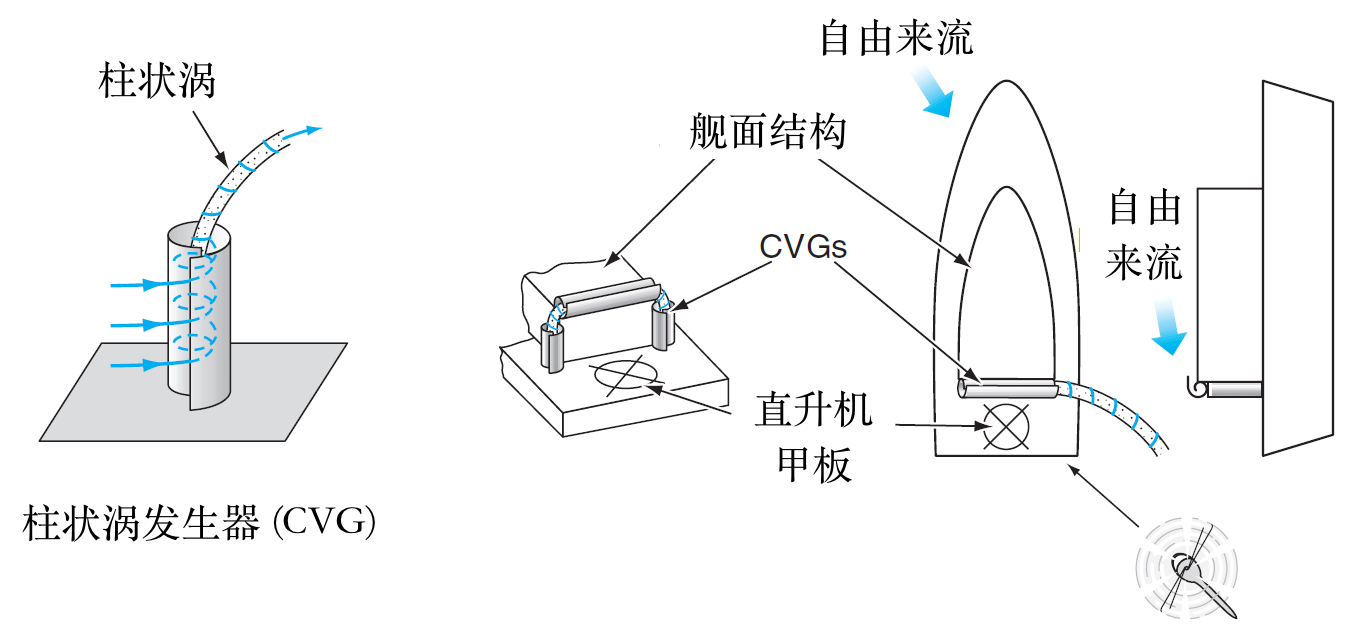
\includegraphics[width=1\textwidth,height=0.24\textheight,keepaspectratio]{../review/figures/modifying}
\caption{\label{fig:CVG}利用柱状涡发生器改善舰载直升机起降环境\upcite{Lamar2004}}
\end{figure}

2011 年,Herry \& Vorst\upcite{Herry2011} 利用 PIV 与激光断层扫描显示技术,在 ONERA
的 L2 风洞中测量了 $1/60$ 简单外形军舰缩比模型和 $1/100$ 真实外形军舰缩比模型两种船体的气流尾迹。

2012 年,Kääriä 等\upcite{Kaeaeriae2012}通过开展水洞试验,研究了直升机在船体气流尾迹中的气动载荷特征。该试验是在一架
$1/54$ 的直升机缩比模型与一艘虽经简化但仍具有机库和飞行甲板的护卫舰模型上进行的,旋翼桨叶被简化为刚性连接到桨毂,气动载荷通过安装在机身内的六分量天平来测量。试验在船头正面迎风与
$\ang{45}$ 侧面迎风两种来流条件下,沿直升机着舰飞行路径选取了若干观测点,测量了直升机在这几个点上的非定常气动载荷。试验结果表明,当船头正面迎风时,甲板上方存在一个拉力不足区域,迫使驾驶员增大总距以保持高度;而在
$\ang{45}$ 侧风条件下,甲板上方存在一堵压力墙,迫使驾驶员减小总距以降低高度、增大横向周期变距以保持飞行路径。他们认为上述现象是由船体气流尾迹的速度梯度引起的,并通过对船体气流尾迹进行非定常
CFD 计算验证了此观点。尽管该试验是在固定直升机的条件下进行的,仍不能完全反映直升机着舰过程的真实载荷特征,但可作为验证计算模型的参照对象。

2015 年,Friedman 等\upcite{Friedman2015}利用固定在(长 $\SI{32.9}{m}$)真实船只尾部甲板上方的模型直升机(如图
\ref{fig:real_ship} 所示),研究了船体气流尾迹与直升机旋翼尾迹的相互影响。通过安置在旋翼周围的风速计,测量了试验船静止、无侧风航行、侧风航行等条件下的流场信息。尽管该试验是在固定直升机的条件下进行的,但已将试验环境从室内转移到了真实的船只上,因而更接近舰载直升机的真实工作环境。
\begin{figure}[h!]
\begin{centering}
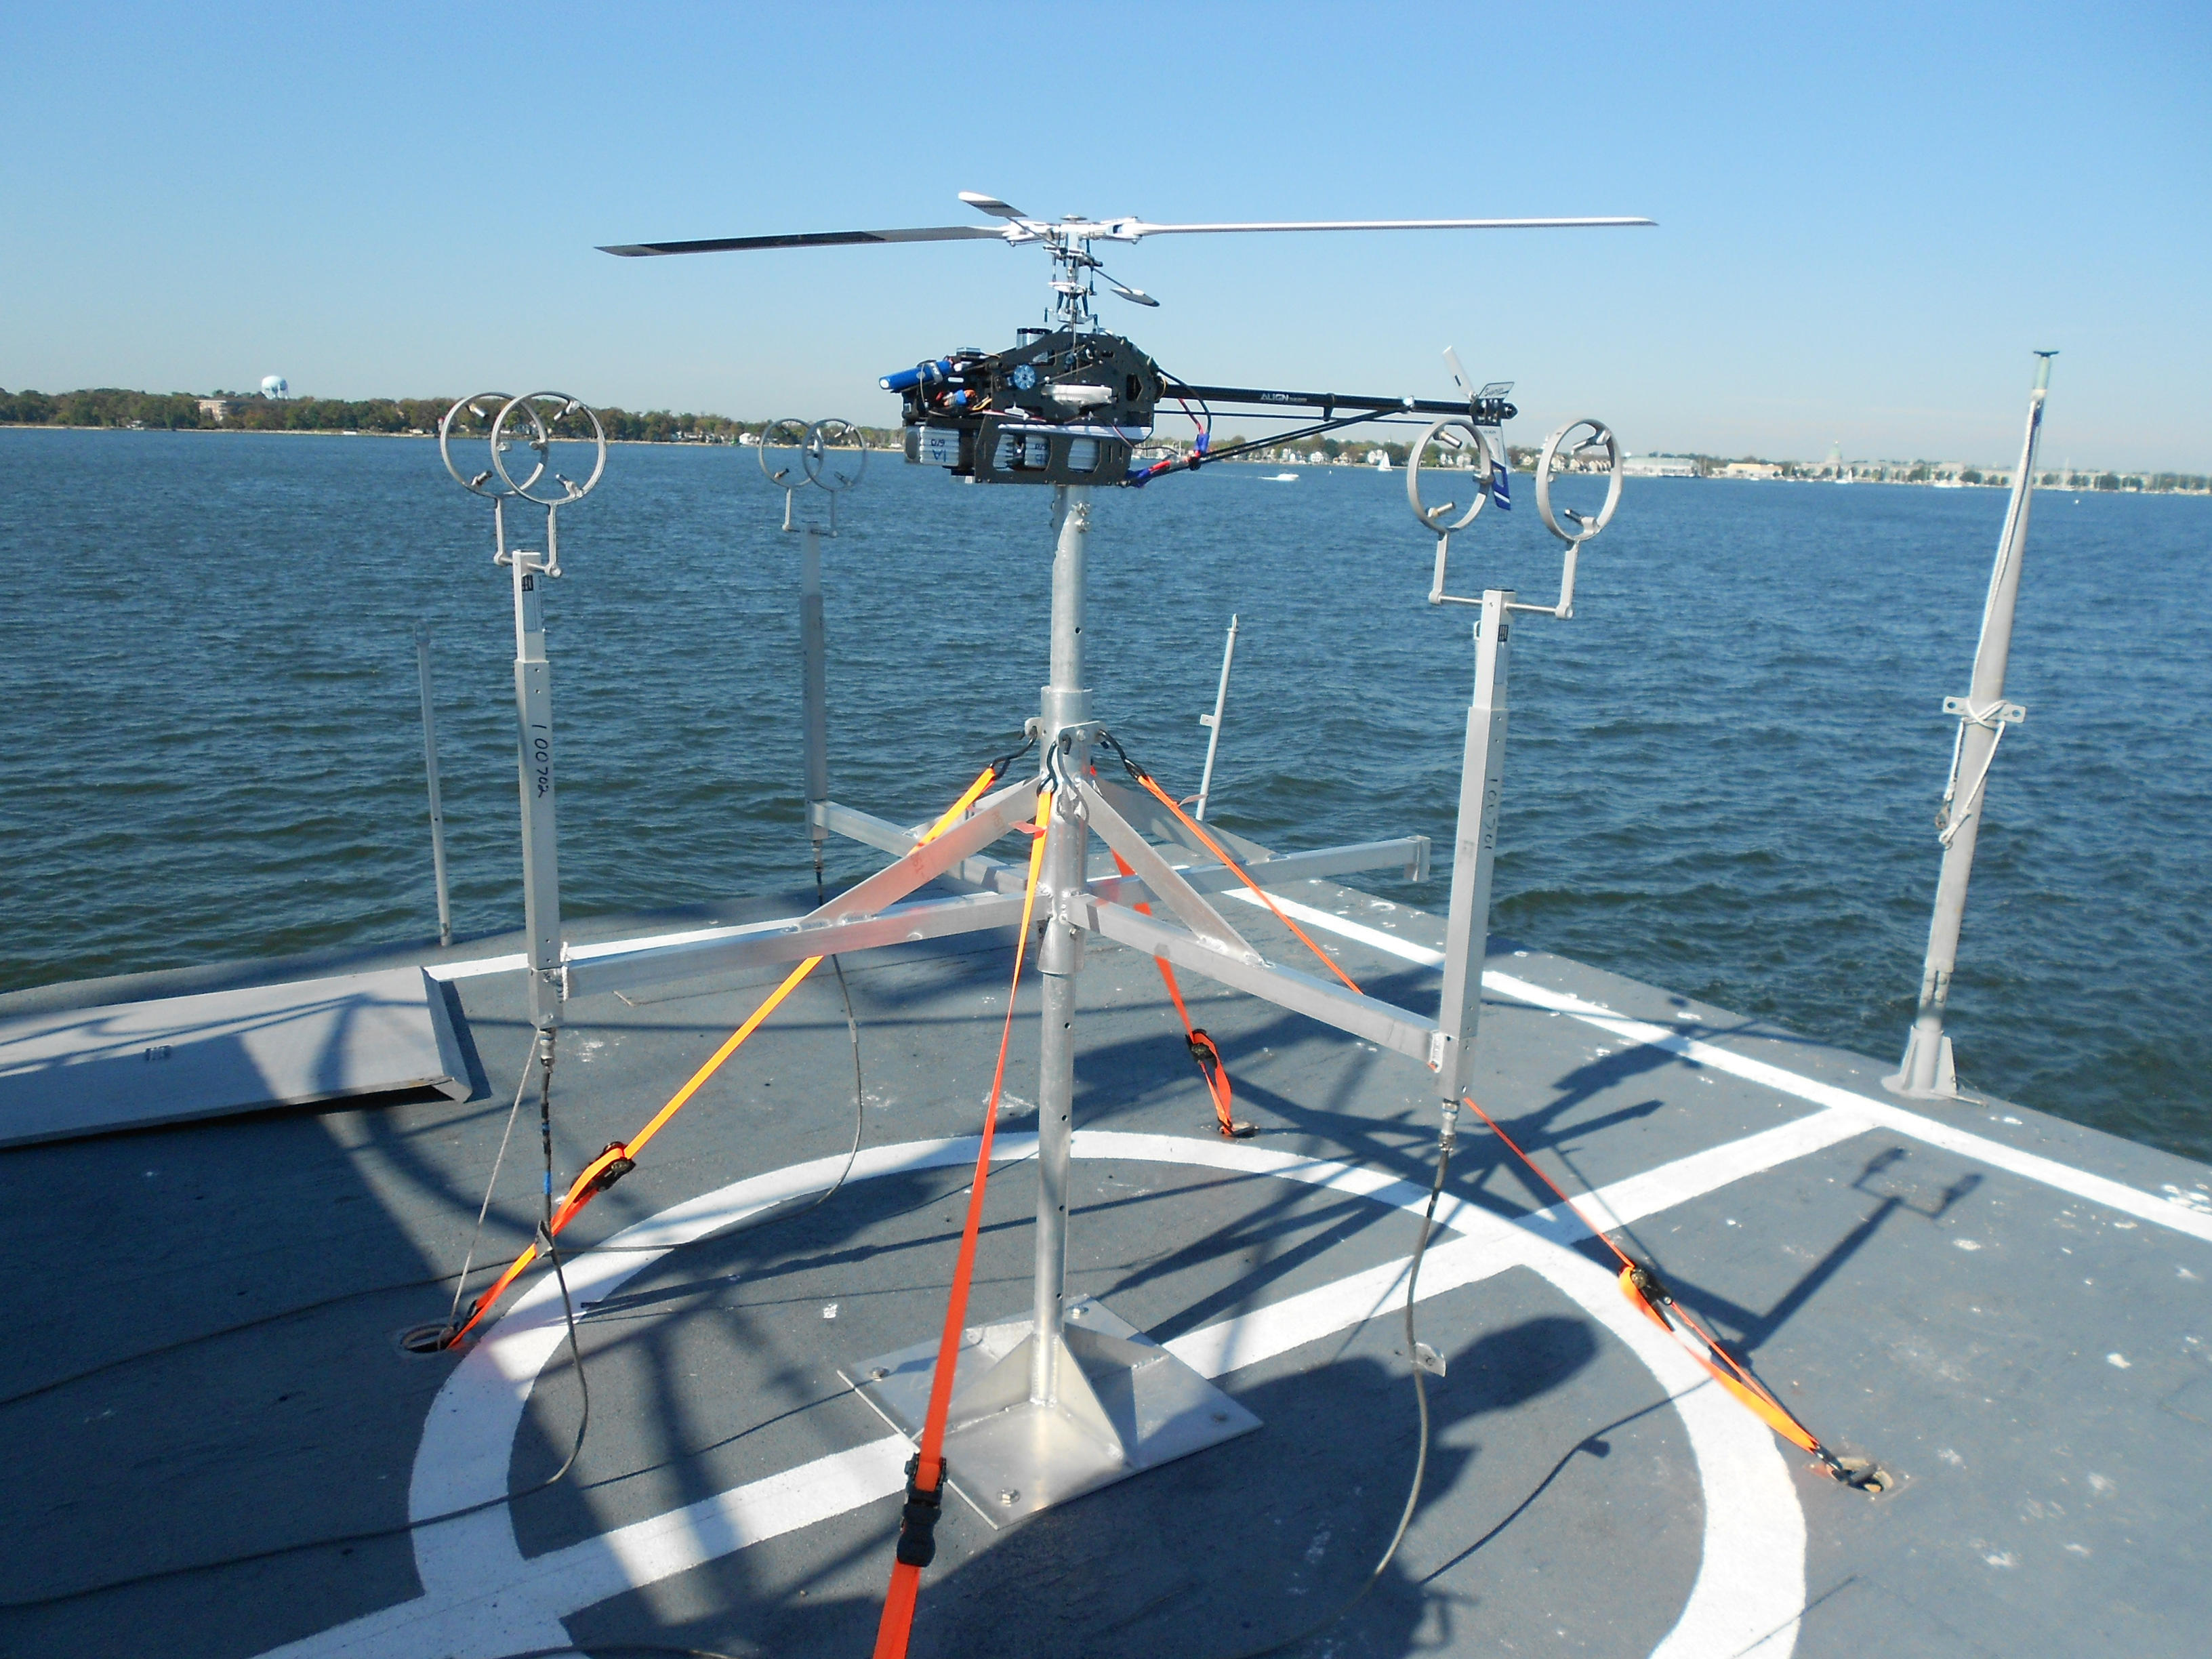
\includegraphics[width=1\textwidth,height=0.33\textheight,keepaspectratio]{/Users/pvc/code/manuscript/review/figures/ship-helicopter-interaction}
\par\end{centering}
\caption{\label{fig:real_ship}固定在真实船只尾部甲板上方的模型直升机\upcite{Friedman2015}}
\end{figure}


\subsection{舰载直升机气动干扰计算}

1995 年,Landsberg 等\upcite{Landsberg1995}利用 FAST3D 非定常流动求解器,分析了船体气流尾迹与旋翼入流的相互作用。该求解器采用的是通量修正输运及虚拟单元嵌入方法。旋翼对流场的影响是通过一个简化的桨盘模型来体现的,该模型中动量源沿桨盘均匀分布,因此只能反映旋翼整体的气动特性,而不能精细到每片桨叶。虽然计算模型较为简单,但计算结果仍能反映船体气流尾迹中的非定常性对旋翼入流的影响。

2008 年,He 等\upcite{He2008}介绍了其所属公司在建立高置信度舰载直升机飞行仿真环境方面所做的工作。该仿真系统集成了直升机动力学、船体动力学以及非定常船体气流尾迹方面的建模方法,为舰载直升机飞行训练和测试提供了一种高效的模拟工具。该仿真系统提供了三种不同精细程度的仿真模型:(1)
旋翼尾迹由有限状态入流模型描述,船体气流尾迹由平板模型描述;(2) 旋翼尾迹由有限状态入流模型描述,船体气流尾迹由 CFD 或试验数据描述;(3)
旋翼尾迹和船体气流尾迹由VPM描述。其中,前两种模型可用于实时仿真计算。此后,该公司的 Zhao 等\upcite{Zhao2013}将
VPM 与基于非结构网格的 CFD 求解器相结合,研究了旋翼尾迹与船体气流尾迹的相互作用。基于此混合方法的计算结果,他们推广了 Peters–He
有限状态入流模型,使其适用于实时仿真。

2013 年,Muijden 等\upcite{Muijden2013}基于结构网格,用 RANS 方程与 RANS/LES\nomenclature{LES}{large eddy simulation}
(large eddy simulation) 混合方法两种物理模型,分析了船体气流尾迹,并与试验数据进行了比较。结果表明:RANS
方程的计算结果很好地反映了船体气流尾迹的时间平均特征,而 RANS/LES 混合方法则进一步给出了更加接近物理真实的流场波动特征。上述计算结果已被用到直升机飞行模拟器中,并且得到了经验丰富的飞行员给出的积极评价。但此文只计算了船体气流尾迹,并没有将直升机(特别是旋翼)包括在计算模型中,因此没有体现船体气流尾迹与旋翼尾迹的耦合效应。

2014 年,Crozon 等\upcite{Crozon2014}基于结构网格,利用作用盘方法对旋翼在船体影响下的入流特征进行了静态计算。作用盘方法的结果表明,当旋翼接近船体时,其入流会受到船体的显著影响,这种影响是非线性的,因而叠加法不再适用。为突破作用盘方法只能描述旋翼整体入流特征的限制,此文通过在滑动结构网格(如图
\ref{fig:sliding-mesh} 所示)上求解非定常 RANS 方程获得了每片桨叶的流场信息。通过该方法得到的旋翼拉力的计算结果与试验结果吻合较好,验证了方法的有效性。他们希望此文的计算方法有助于确定直升机着舰过程的安全飞行包线,但并没有给出具体的结论。就算例而言,此文只研究了孤立旋翼与船体的气动干扰,没有考虑机身对气流的影响。
\begin{figure}[h!]
\begin{centering}
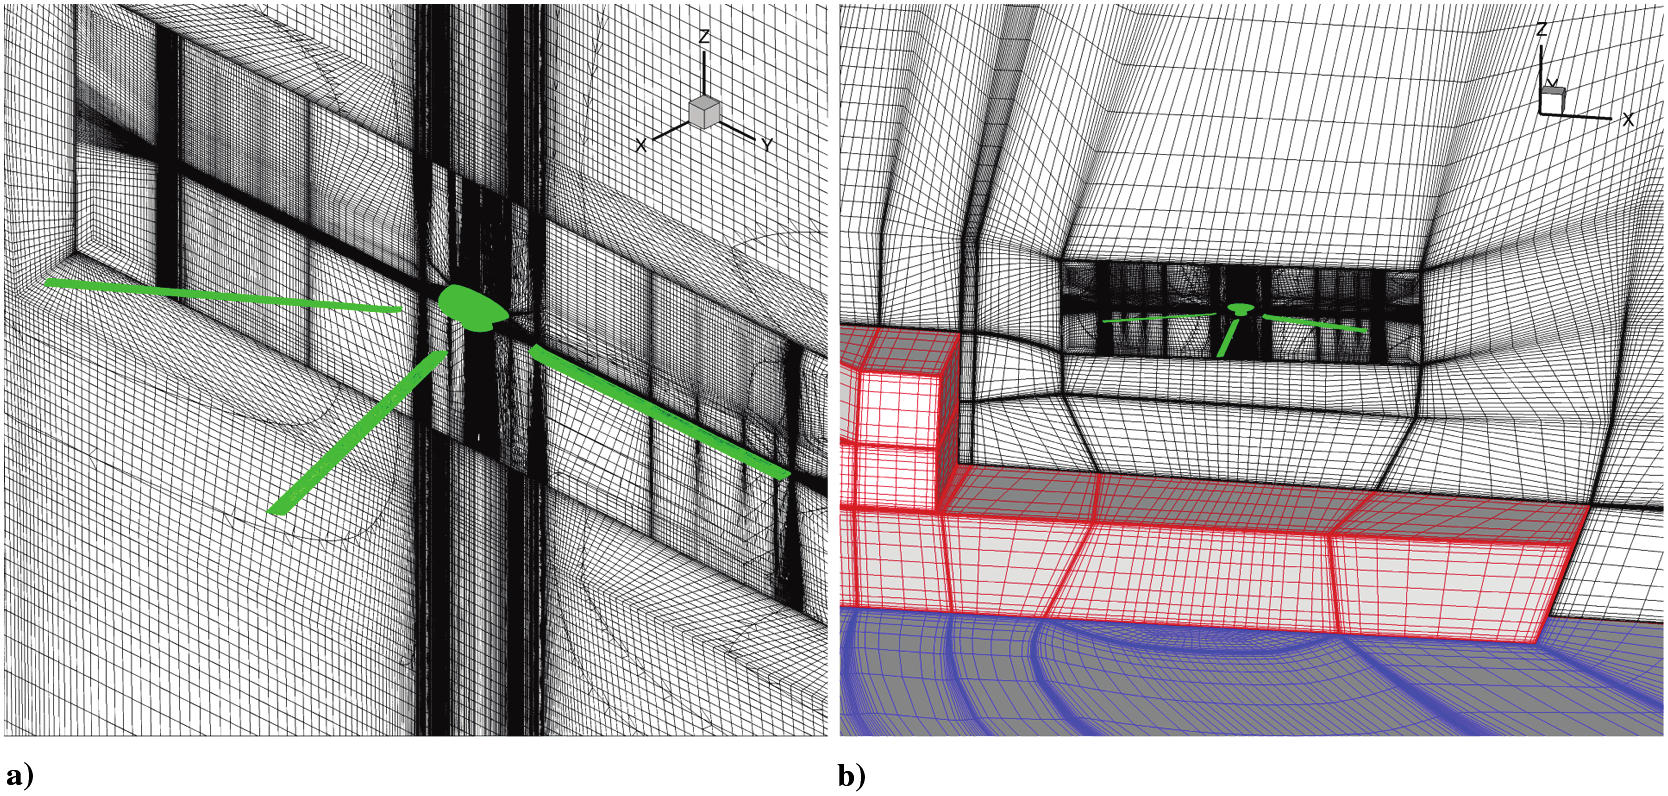
\includegraphics[width=1\textwidth,height=0.3\textheight,keepaspectratio]{../review/figures/structured_sliding_mesh}
\par\end{centering}
\caption{\label{fig:sliding-mesh}用于计算旋翼–船体非定常气动干扰的滑动结构网格\upcite{Crozon2014}}
\end{figure}

2017 年,南京航空航天大学的史勇杰等\upcite{Shi_2017}利用重叠网格技术(如图 \ref{fig:overset-mesh}
所示),研究了孤立旋翼与多种船体构型之间的气动干扰问题。他们用静态结构网格离散船体周围的空间,作为背景网格;用 C-O 或 C-H
型结构网格包裹桨叶,作为贴体网格。贴体网格被允许在背景网格中做任意运动,以模拟桨叶的旋转、挥舞、变距。两套网格上的数据通过三维线性插值进行交换。该方法在进行挖洞和贡献单元搜索时,利用了结构网格易于定位单元的性质,所需时间与流场计算时间相比可忽略不计。这种对结构网格的依赖,限制了该方法的适用范围。
\begin{figure}[h!]
\begin{centering}
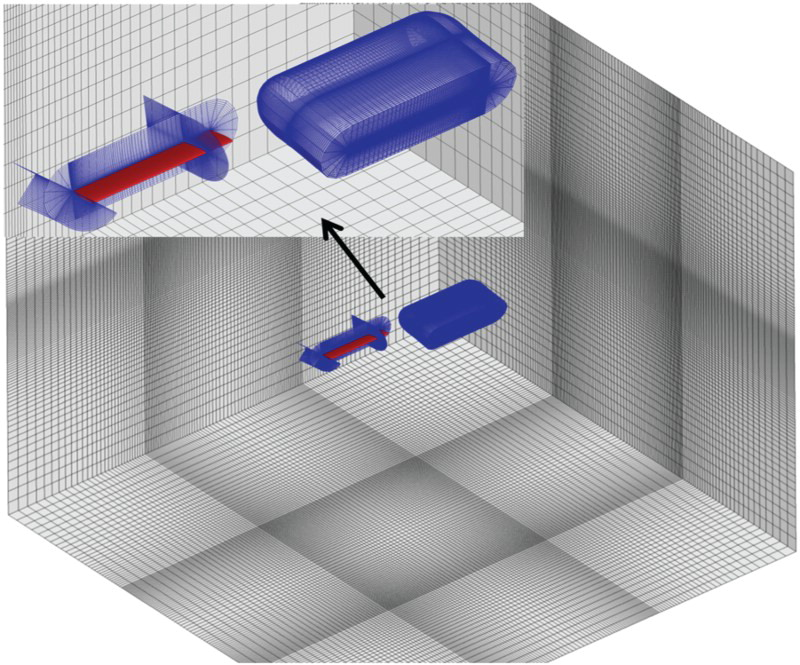
\includegraphics[width=1\textwidth,height=0.32\textheight,keepaspectratio]{figures/overset_mesh.jpeg}
\par\end{centering}
\caption{\label{fig:overset-mesh}用于计算旋翼–船体非定常气动干扰的重叠结构网格\upcite{Shi_2017}}
\end{figure}


\subsection{受气动干扰影响的工程问题}

在舰载直升机的实际工程应用中,人们通常更关注其飞行安全性与驾乘舒适度,这就需要从结构动力学、飞行动力学、导航与飞控等学科的视角对舰载直升机开展研究。这些学科或多或少都需要以气动载荷作为输入,因此可以被视为舰载直升机空气动力学的下游学科。最理想情况当然是将基于
PIV 或 CFD 的精细空气动力学模型植入到结构动力学、飞行动力学模型中。然而现实情况却是上下游学科的研究存在明显脱节,工程领域往往还在使用陈旧且粗糙的气动模型,有些学科甚至直接将气动力作为黑箱或随机过程处理。这种脱节说明舰载直升机空气动力学的研究成果尚未充分发挥其价值,应当引起上下游学科的共同关注。

\subsubsection{结构动力学}

Wei 等\upcite{Wei1992}于 1992 年分析了 SH-2F 型直升机在预定的甲板运动、甲板摩擦、定常风条件下的结构动力学特性,用以确定该型直升机安全着舰和离舰的条件。对处于工作状态的旋翼、处于非工作状态的旋翼、折叠起来的旋翼以及机身分别进行了建模,以研究这4种情况的空气动力学特性。利用能量法推导了船体运动的动力学方程,包含三个线位移、两个角位移(滚转、俯仰)共五个自由度。此外,他们还分析了不同甲板摩擦条件对直升机结构动力学特性的影响。基于上述分析模型,此文给出了一些定性和定量的安全指标,但有待试验数据的验证。

Wall\upcite{Wall2009} 于 2009 年研究了直升机着舰和离舰过程中桨叶特有的气动弹性问题。在海上风速较大且旋翼转速较低时,桨叶容易出现较大变形,这是由桨叶的动力学特性、船体运动、船体气流尾迹等因素共同作用所引起的。他们将柔性桨叶离散为若干刚性的微段,用以表现非线性的桨叶弯曲变形;基于试验数据对船体气流尾迹进行建模,体现了甲板上方气流随时间、空间变化的非定常、非均匀的特征。此文反映了影响桨叶气弹响应的各种因素之间相互作用关系的复杂性,但分析所用气动模型依赖试验数据,可考虑用更一般的
CFD 方法代替。

\subsubsection{飞行动力学}

1986 年,Jewell 等\upcite{Jewell1986}介绍了一项由美国海军航空发展中心支持的试验研究。该项研究的目的是在直升机操稳参数、舰面操纵流程、环境条件等方面,对飞行品质规范的修订提出建议。

Clement 等\upcite{Clement1992}于 1992 年建立了一种用于模拟直升机着舰飞行的实时仿真模型。该模型采用叶素法对旋翼进行气动建模;利用
CFD 软件得到船体气流尾迹数据,并经过三维快速傅里叶变换算法处理,使其适用于实时仿真。

1994 年,Zhang 等\upcite{Zhang1994}利用全尺寸海上试验数据,识别出了一个关于船体气流尾迹速度垂直分量的功率谱模型。基于上述半经验的船体气流尾迹模型和一个简化的旋翼气动模型,他们研究了船体气流尾迹对旋翼拉力和滚转、俯仰力矩的影响。此后,他们又建立了一种用于模拟直升机与船体气动干扰并考虑地面效应的实时仿真模型。该模型中,船体由板块表示,旋翼尾迹由固定尾迹和预定尾迹模型表示,海面的影响(地面效应)通过镜像法体现。基于以上模型,将旋翼入流表示成有限状态形式,以便于进行实时仿真。该模型只适用于直升机在甲板上方悬停的配平问题。此后,他们还对直升机与船体气动干扰问题中的地面效应问题进行了研究\upcite{Zhang1995}。

1999 年,Bogstad 等\upcite{Bogstad1999,Bogstad2002}利用基于欧拉方程和非结构网格的有限元求解器,研究了船体气流尾迹,并将得到的数据整合到直升机飞行仿真软件中。Zan\upcite{Zan2003}
于 2003 年对文献 \cite{Bogstad2002} 中的一些观点提出了质疑,其认为特殊算例的计算结果与试验数据进行的对比,并不能证明该方法在更一般的条件下仍然有效;试验和基于
Navier–Stokes 方程的计算结果都显示,在某些情况下,船体气流尾迹是由涡流主导的,并且存在强烈的流动分离现象,因此文献 \cite{Bogstad2002}
中基于 Euler 方程得到的结论并不可靠。

\newpage{}

2003–2005 年,Lee 等\upcite{Lee2003,Lee2005}基于非结构网格,利用无黏 CFD 计算得到船体气流尾迹,并将其引入到直升机飞行仿真程序
GENHEL 中。基于此模型,他们针对特定的直升机着舰和离舰飞行轨迹,设计了最优控制算法。结果表明,船体气流尾迹的非定常性对于直升机着舰和离舰操纵具有显著影响,这正是舰载直升机与舰载固定翼飞机明显不同的地方。此文中的
CFD 计算模型没有考虑空气黏性,因而丢失了一些真实船体气流尾迹的特征。在后续研究\upcite{Lee2004}中,他们引入了一种随机船体气流尾迹模型,用以提高仿真的效率。该模型可用于优化飞行控制系统,以提高飞行器抗干扰性能。

2006 年,Hoydonck 等\upcite{Hoydonck2006}建立了一种用于模拟直升机着舰操纵的飞行力学模型。旋翼模型采用刚性桨叶,考虑二阶挥舞运动,用叶素法对主旋翼进行建模。旋翼入流采用一种改进的
Pitt–Peters 动态入流模型进行建模,通过引入四个状态变量来体现尾迹畸变对旋翼入流的影响。利用该模型,他们研究了直升机按预定路径着舰的飞行稳定性和控制问题,但并没有考虑船体空气尾流对旋翼的影响。

2007 年,Akinyanju\upcite{Akinyanju2007} 基于直升机综合分析软件 FLIGHTLAB,对舰载直升机舰面操纵进行了建模和分析,并将仿真结果与试验数据进行了比较。他们采用叶素法、有限状态尾迹和自由尾迹对旋翼进行建模,基于
CFD 对船体气流尾迹进行模拟,引入地面涡模拟甲板和海面引起的地面效应。计算结果表明:船的航行速度、航向、旋翼转速、海况对直升机的舰面操纵具有显著影响,并且得到了试验数据的验证。但此文中的建模工作过于依赖该软件提供的功能,因而不具有一般性,也不易引入更精细的空气动力学或结构动力学模型。

2012 年,Forres 等\upcite{Forrest2012}将非定常 CFD 计算所得的船体气流尾迹数据引入到直升机飞行模拟器中,得到了一个比较接近真实情况的飞行仿真环境。一些直升机着舰过程中真实存在的现象,在该仿真模型中得到了体现。通过飞行员的主观评价以及其他客观指标,验证了该模型的有效性,也验证了将船体气流尾迹
CFD 计算结果引入飞行仿真的可行性。尽管该方法只考虑了船体空气尾流对旋翼尾迹的影响,但仍可应用于舰载直升机飞行员的日常训练。

\subsubsection{导航与飞控}

1991 年,Negrin 等\upcite{Negrin1991}介绍了一种用于手动执行直升机在移动甲板上方低空悬停任务的叠加显示技术。分析和试验结果表明,将惯性参考系中的位置信息提供给飞行员,有助于提高直升机在移动甲板上方执行悬停任务的质量。该研究以线化方程表示直升机运动,以马尔可夫过程模拟大气扰动,因此并没有将空气动力学的研究成果引入其中。

2005 年,Hess\upcite{Hess2005} 基于简化的船体运动和直升机飞行动力学模型,提出了一种适用于直升机全包线飞行控制系统设计的方法,并将该方法应用于直升机在高速航行的船只甲板附近执行位置保持任务。该模型将大气扰动的影响表示为传递函数,后者基于
UH-60 直升机的飞行试验数据而获得,因此间接利用了气动试验研究的成果。 

2014 年,Ngo \& Sultan\upcite{Ngo2014} 建立了一种用于着舰操纵的面向控制系统设计的非线性直升机飞行力学模型。该模型具有隐式常微分方程的形式,其结果与基于悬停和前飞状态线化模型的结果吻合较好。此外,他们用一种简单的船体运动模型来模拟海面不规则运动对船体的影响。基于以上直升机模型和船体模型,他们利用模型预测控制方法,设计了一种能够完成自主着舰任务的控制系统。从工程实践角度看,该模型具有一定的应用价值,但其所用的
Pitt–Peters 入流模型,并没有考虑旋翼与船体之间的气动干扰。

\subsection{国内外研究现状小结}

舰载直升机空气动力学的研究内容,既包括所有直升机的共性问题,也包括海上作业带来的特殊问题。对共性问题的研究属于旋翼空气动力学的范畴,其主要任务是认识旋翼流场的特征,为结构动力学、飞行动力学等下游学科提供气动模型。对特殊问题的研究则是舰载直升机空气动力学的侧重点,其主要任务是研究海面、船体与旋翼之间的气动干扰规律,为提高舰载直升机海面作业的安全性、舒适性提供支持。

对旋翼乃至舰载直升机空气动力学的试验研究经历了从定性到定量、从宏观到微观的发展过程。定量试验包含测力试验和测速试验两类。伴随试验技术的进步,测速试验经历了介入式测速(HWA
技术)、非介入式单点测速(LDV 技术)、非介入式多点测速(PIV 技术)的发展过程。目前,三维 PIV 技术已经能够在全尺寸亚声速风洞{[}84{]}中对旋翼流场进行高分辨率测量。可以预见,该技术在未来一段时间里仍将是旋翼空气动力学研究的重要工具。

数值计算是旋翼乃至舰载直升机空气动力学的另一类重要的研究方法。旋翼流场的非定常、非线性特征决定了问题的复杂性。为了真实还原旋翼流场的流动特征,必须解决好转捩、附面层分离、涡核粘性耗散、涡结构失稳破裂等复杂的流体力学问题。为了解决网格离散带来的涡量非物理耗散问题,网格自适应加密技术、涡量约束方法等新兴的流体力学计算方法正成为该领域的研究热点。

尽管舰载直升机空气动力学的研究已经用上 PIV、CFD 等先进技术,但其所积累的研究成果尚未广泛应用到结构动力学、飞行动力学、导航与飞控等以气动载荷作为输入的下游学科。近些年来,随着人工智能算法的不断改进以及计算机软硬件水平的稳步提升,直升机飞控系统的设计正朝着无人自主控制的方向迈进(美国已实现无人直升机的海上自动起降)\upcite{DengJingHui_2021}。

\newpage{}

\section{研究内容}

\subsection{船体气流尾迹计算方法}

舰载直升机气动问题与路基直升机气动问题的主要区别,在于船体气流尾迹的存在及其对旋翼尾迹的影响。

单纯的船体气流尾迹问题,与 CFD 文献中常见的圆柱绕流问题具有相同的物理背景。因此,适用于后者的计算方法,原则上都可以用来计算船体气流尾迹。由于圆柱具有简单的几何外形,为其生成结构网格较为容易,因此大多数用于计算圆柱绕流的求解器,都是基于有限差分格式。这类格式构造简单、易于升阶,但只适用于结构网格。然而在实际工程应用中,船体通常具有复杂的几何外形,这为结构网格的生成带来了非常大的困难。

得益于计算几何的发展,非结构网格能够在具有复杂几何外形的区域内自动生成,因此适用于船体气流尾迹的计算。但适用于非结构网格的计算方法,通常需要引入较为复杂的数据结构,因此比有限差分格式更难实现。另一方面,在非结构网格上构造的计算格式,通常不易提升精度阶数,这大大降低了非结构网格计算结果的参考价值。

寻找并实现一种在非结构网格上易于构造高阶格式的 CFD 方法,是本文要解决的首要问题。

\subsection{旋翼空气动力学模型}

不同旋翼空气动力学模型的主要区别,在于如何反映旋转的桨叶对流场的非定常扰动。

基于拉格朗日观点的涡元法(如:自由尾迹模型、涡粒子模型),将流场的涡量分布表示为一系列离散的涡量单元。这些涡元生成于旋转的桨叶上,从桨叶后缘脱落后随当地气流自由运动。在不考虑边界条件或边界条件足够简单(如平直大地)的情况下,这类模型(相对于
CFD 方法)能够高效地模拟桨叶的非定常运动及旋翼尾迹的动态变化。但这类模型通常难以植入现有的 CFD 方法,因此不适合于舰载直升机气动干扰问题的研究。

基于欧拉观点的连续介质模型(如:涡量输运方程、Navier–Stokes 方程),将桨叶视为移动的固壁边界。为了在这些移动固壁上施加边界条件,通常需要借助变形网格、滑动网格、重叠网格等动态网格技术。与不含移动固壁边界从而可以使用静态网格的常规
CFD 问题相比,使用动态网格技术必然会带来计算量的剧增。

提出并验证一种既能处理具有复杂外形的边界,又能模拟桨叶的非定常运动,还能避免使用动态网格技术的旋翼空气动力学建模方法,是本文研究的主要内容。

\subsection{算法的并行加速}

舰载直升机气动干扰问题属于复杂流动问题,无论采用何种计算模型,都需要消耗大量的计算资源。为了提高问题的求解效率,扩大问题的求解规模,必须对算法做并行加速。为了评估加速的效果,需要在具体的计算设备上进行测试,以确定性能瓶颈和进一步改进的方向。

“消息传递接口 (message passing interface, MPI\nomenclature{MPI}{message passing interface})”是目前最主流的并行计算标准,几乎所有高性能计算平台上都部署了该标准的某种具体实现。应用程序通过调用它提供的函数,将计算任务发送到各个计算节点(核心)上做并行处理,从而扩大求解规模、提高计算效率。MPI
技术基于粗粒度的进程级并行,对单核性能的要求较低,具有良好的可移植性和可扩展性。

利用 MPI 技术实现对既有算法的并行加速,是本文对前人工作的一大改进。

\section{全文结构}

本文共分为五章,各章内容安排如下:

第\ref{chap:=007EEA=008BBA}章为绪论,首先介绍本文的研究背景,随后综述国内外研究现状,并提出本文的研究内容,最后给出全文的组织结构。

第\ref{chap:=007B97=006CD5}章推导一种适用于三维非结构网格、能够有效压制数值振荡的“Runge–Kutta
间断 Galerkin (RKDG)”有限元方法/求解器。在此基础上,将一种“非定常动量源 (unsteady momentum source,
UMS)”模型与该方法/求解器相结合,提出一种支持对旋翼空气动力学问题进行高效、高精度数值模拟的 UMS–RKDG 方法/求解器。

第\ref{chap:=009A8C=008BC1}章利用具有解析解或精确解的一维标准算例,定量验证上述 RKDG 求解器的正确性和精度阶数。利用拥有公认数值解的二维标准算例,定性验证上述求解器捕捉复杂流动图象的能力。

第\ref{chap:=005E76=00884C}章对上述求解器做了并行加速,以支持高性能计算平台上的分布式并行计算。基于并行化的
UMS–RKDG 求解器,开展爬升、前飞两种工况的旋翼数值风洞试验,定性验证 UMS–RKDG 近似解的正确性和高精度优势。在此过程中,对上述求解器的并行性能进行了测量和评估。

第\ref{chap:=005E94=007528}章利用上述经过验证的 UMS–RKDG 求解器,模拟了一种简化条件下的单旋翼–船体–海面气动干扰的形成过程。结果表明:本文提出并实现的上述求解器,能够在较粗的网格上捕捉到单旋翼–船体–海面气动干扰的主要流场特征,可用于更复杂的舰载直升机气动干扰问题研究。

最后是结论部分,总结了本文的主要内容及创新点,并对进一步研究的方向给出了建议。

\chapter{舰载直升机三维流场的高阶计算格式\label{chap:=007B97=006CD5}}

目前在航空航天工程中使用的大多数 CFD 求解器都是基于有限体积格式。有限体积格式可以在非结构网格上构造,因此比有限差分格式更容易处理具有复杂几何外形的流场边界。然而,有限体积格式通常只有二阶空间精度,这是由于不规则局部模板的尺寸随着精度的阶数增加而迅速增长。在高阶有限体积格式中,单元的本地模板由单元和单元的邻居、邻居的邻居等组成。为了简化非结构网格上的高阶格式的设计,最好使用局部模板比有限体积格式更紧致的有限单元法,如:“间断伽辽金
(discontinuous Galerkin, DG)”法。DG 法在每个单元内部用连续函数做近似(这一点更像经典有限元法),但允许在单元边界上存在间断(这一点更像经典有限体积法)。这样的假设使格式设计者在为每个单元选择基函数时有更大的自由度,例如:基于正交基函数的模态型
DG 法,基于拉格朗日多项式的节点型 DG 法\upcite{Hesthaven_2008}。

最早的 DG 格式由 Reed \& Hill\upcite{Reed_1973} 引入,用于求解中子输运方程。这是一个仅包含一阶空间导数的线性问题。对于非线性守恒律,Chavent
\& Salzano\upcite{Chavent_1982} 首次尝试使用 DG 法进行空间离散,并使用显式 Euler 格式进行时间离散。该格式在空间上是二阶精度的,但在时间上只有一阶精度。为了提高时间离散的精度,Cockburn
\& Shu\upcite{Cockburn_1988} 将一阶 Euler 格式替换为某种特殊的二阶 Runge–Kutta (RK\nomenclature{RK}{Runge–Kutta})
格式\upcite{Shu_1988,Shu_1989},所得格式是“总变差递减的 ( total variation diminishing,
TVD)”。它是第一个取得成功的 RKDG 格式,该格式在空间和时间上都具有高阶精度,适用于标量守恒定律。这种方法很快被推广到一维守恒律方程组\upcite{Cockburn_1989}、高维标量守恒律\upcite{Cockburn_1990}以及高维守恒律方程组\upcite{Cockburn_1998},包括描述无黏可压流的
Euler 方程。几乎在同一时期(1990 年代后期),DG 法也被扩展到控制黏性流动的 Navier–Stokes 方程。Bassi
\& Rebay\upcite{Bassi_1997} 首次尝试将 DG 离散应用于未知量及其梯度,以求解 Navier–Stokes
方程。该方法随后被 Cockburn \& Shu\upcite{Cockburn_1998b} 推广为局部 DG 法,将 RKDG
方法从守恒律推广到对流占优问题,具体推广过程可参考文献 \cite{Cockburn_2001}。

RKDG 方法虽然能在非结构网格上构造出高阶格式,但对于含有移动边界(如:旋翼桨叶)的问题,通常需要使用动态网格技术(例如变形网格、滑动网格、重叠网格)。另一方面,在有限差分及有限体积法中,典型的升力体(如:旋翼)已成功地被建模为各种形式的动量源。Rajagopalan
\& Mathur \upcite{Rajagopalan_1989,Rajagopalan_1993} 提出了第一个基于有限差分及有限体积的动量源模型,该模型将旋翼的时间平均效应建模为作用盘。北航的康宁和孙茂\upcite{Kang_1997,Kang_2000}用这种时间平均的动量源模型,模拟了处于地面效应中的旋翼的流场。南航的史勇杰等\upcite{Shi_2017}将该模型与非定常重叠网格方法进行了比较,发现定常动量源模型能够以更低的计算成本模拟旋翼和飞行甲板之间的复杂气动干扰。Shen\upcite{Shen_2009}
和 Kim\upcite{Kim_2015}用代表各片桨叶的作用面模型,捕获了旋翼流场的非定常效应。此类早期工作要么通过忽略非定常效应而过度简化(如文献 \cite{Rajagopalan_1989,Rajagopalan_1993,Kang_1997,Kang_2000}),要么仅限于结构网格(如文献 \cite{Shen_2009,Shi_2017})。

本章将前人为解决二维守恒律问题而提出的带有紧致型 WENO 限制器的 RKDG 方法,推广为含有源项的三维双曲型方程组的求解方法,并在最后一节给出一种特殊的源项,用以模拟旋翼对流场的非定常扰动。

\section{三维非结构网格上的 DG 空间离散\label{sec:DG}}

\subsection{非结构网格}

离散某空间区域最常用的方法,是将该区域分割为有限个互不重叠的“单元 (element/cell)”。这些单元通常具有简单的几何外形,例如:直线段、三角形、四边形、四面体、三棱柱、六面体。定义单元所用到的几何点被称为“结点
(node/point)”,由多个单元共享的结点被称为“顶点”,由某个单元独占的结点被称为“内点”。记录所有单元及结点信息的数据结构被称为“网格
(mesh/grid)”。为方便叙述,表 \ref{tab:mesh} 列出了本文用到的网格术语及记号,其中“对象 $X$”指代由网格成员组成的任意子集。
\begin{table}
\centering{}\caption{\label{tab:mesh}网格术语及记号}
\begin{longtable}[c]{ccccc}
\toprule 
中文名 & 英文名 & 记号 & 简写 & 含义\tabularnewline
\midrule
网格 & Grid & $G(\varOmega)$ 或 $G_{\varOmega}$\nomenclature{$G(\varOmega)$ 或 $G_{\varOmega}$}{表示覆盖区域 $\varOmega$ 的网格}  & $G$ & 用于离散空间区域 $\varOmega$ 的网格\tabularnewline
索引 & Index & $I(X)$ 或 $I_{X}$\nomenclature{$I(X)$ 或 $I_{X}$}{表示对象 $X$ 中所有成员编号之集} & $I$ & 对象 $X$ 中所有成员编号之集\tabularnewline
总数 & total Number & $N(X)$ 或 $N_{X}$\nomenclature{$N(X)$ 或 $N_{X}$}{表示对象 $X$ 中所有成员的数量} & $N$ & 对象 $X$ 中所有成员的总数\tabularnewline
体单元 & Volume element & $V(X,i)$\nomenclature{$V(X,i)$ 或 $V_{i}$}{表示对象 $X$ 中的第 $i$ 号体单元} & $V_{i}$ & 对象 $X$ 中的第 $i$ 号体单元\tabularnewline
 &  & $V(X)$ 或 $V_{X}$\nomenclature{$V(X)$ 或 $V_{X}$}{表示对象 $X$ 中的所有体单元} & $V$ & 对象 $X$ 中的所有体单元\tabularnewline
面单元 & Surface element & $S(X,i)$\nomenclature{$S(X,i)$}{表示对象 $X$ 中的第 $i$ 号面单元} & $S_{i}$ & 对象 $X$ 中的第 $i$ 号面单元\tabularnewline
 &  & $S(X)$ 或 $S_{X}$\nomenclature{$S(X)$ 或 $S_{X}$}{表示对象 $X$ 中的所有面单元} & $S$ & 对象 $X$ 中的所有面单元\tabularnewline
结点 & Point & $P(X,i)$\nomenclature{$P(X,i)$}{表示对象 $X$ 中的第 $i$ 号结点} & $P_{i}$ & 对象 $X$ 中的第 $i$ 号结点\tabularnewline
 &  & $P(X)$ 或 $P_{X}$\nomenclature{$P(X)$ 或 $P_{X}$}{表示对象 $X$ 中的所有结点} & $P$ & 对象 $X$ 中的所有结点\tabularnewline
\bottomrule
\end{longtable}
\end{table}

从几何的角度看,网格应恰好填满整个区域,即\nomenclature{$\varOmega$}{表示计算区域}
\begin{equation}
\varOmega=\bigcup_{i\in I_{V(G)}}\overline{V_{i}},
\end{equation}
且相邻体单元之交的体积为零,即\nomenclature{$\delta_{ik}$}{表示 Kronecker 记号,$i=k$ 时取值为 $1$,否则取值为 $0$}

\newpage{}

\begin{equation}
\int_{V_{i}\cap V_{k}}1=\delta_{ik}\int_{V_{i}}1,\qquad\forall(i,k)\in I_{V(G)}\times I_{V(G)},
\end{equation}
其中 $\overline{V_{i}}\coloneqq V_{i}\cup(\partial V_{i})$ 为 $V_{i}$
之“闭包 (closure)”。\nomenclature{$\overline{V_{i}}$}{表示体单元 $V_{i}$ 的闭包}\nomenclature{$\partial V_{i}$}{表示体单元 $V_{i}$ 的边界}若无特殊说明,本文所称“体单元”均指开集。

从数据结构的角度看,网格是所有体单元、面单元、结点的“容器 (container)”,体单元又是其所拥有的面单元、结点的容器,因此这些容器应当支持对其成员的快速“遍历
(traversal)”,即复杂度不超过 $N_{X}\lg^{3}N_{X}$,这里的 $N_{X}$ 为容器 $X$ 的成员数量。除此之外,面单元应当支持对其两侧体单元的快速“查询
(query)”,即复杂度不超过 $\lg^{3}N_{V}$,这里的 $N_{V}$ 为体单元数量。

除上述条件外,有限体积法、有限单元法对网格没有更多的要求,因此特别适合于“非结构 (unstructured)”网格,从而特别适合于具有复杂几何边界的问题。这种网格的灵活性正是有限体积法、有限单元法相对于有限差分法的优势之一。在连续介质力学中,“控制体
(control volume)”与“控制面 (control surface)”具有重要的物理意义。最自然的方案是:以体单元为控制体、以面单元为控制面。

对于一维问题,最简单的网格方案是一维结构网格:用 $N_{P}$ 个结点将一维区间 $[a,b]$ 分割为首尾相连的 $N_{V}=N_{P}-1$
个控制体,即
\begin{equation}
\varOmega\coloneqq[a,b],\qquad P(G)=\left\{ P_{i}\coloneqq x_{i}\right\} _{i=1}^{N_{P}},\qquad V(G)=\left\{ V_{i}\coloneqq(x_{i},x_{i+1})\right\} _{i=1}^{N_{V}},
\end{equation}
以相邻控制体的公共端点为控制面,因此 $P_{i}\equiv S_{i}$。对于静态网格(在计算过程中保持不变的网格),最简单的数据结构(数组)即可满足前述条件。在更一般的一维非结构网格中,结点编号可能相当无序,即不要求
$i<j\iff x_{i}<x_{j}$,而是记 $V_{i}\coloneqq(x_{i-1/2},x_{i+1/2})$,其中
$x_{i\pm1/2}$ 表示控制体 $V_{i}$ 两端点的坐标值。\nomenclature{$x_{i-1/2}$}{表示一维网格中第 $i$ 号单元的左端点}\nomenclature{$x_{i+1/2}$}{表示一维网格中第 $i$ 号单元的右端点}按此记法,\nomenclature{$\vert V_{i}\vert$}{表示单元 $V_{i}$ 的测度(线单元的长度、面单元的面积、体单元的体积)}$V_{i}$
的长度(一维体积)可以记为
\begin{equation}
h_{i}\coloneqq\vert V_{i}\vert\coloneqq\int_{V_{i}}1=\int_{x_{i-1/2}}^{x_{i+1/2}}1\dd{x}=x_{i+1/2}-x_{i-1/2}.
\end{equation}

对于高维问题,网格的生成是一项重要且相对独立的技术,需要借助专业的软件(例如:\href{http://gmsh.info/}{Gmsh}、\href{https://www.cgal.org/}{CGAL})来完成。这些软件输出的非结构网格文件(例如:\href{http://gmsh.info/doc/texinfo/gmsh.html\#File-formats}{MSH}、\href{https://www.vtk.org/wp-content/uploads/2015/04/file-formats.pdf}{VTK}、\href{http://cgns.github.io/}{CGNS})通常只含有结点坐标与体单元结点编号等信息,而不会显式记录面单元及其与体单元的关联信息。在导入这类网格文件时,需要以
$\order{N_{V}\lg^{3}N_{V}}$ 复杂度构造所有面单元,并为每个面单元创建其相邻体单元的引用\footnote{\href{https://www.openfoam.com}{OpenFOAM} 定义的 \href{https://www.openfoam.com/documentation/user-guide/4-mesh-generation-and-conversion/4.1-mesh-description}{polyMesh 格式}会显式记录面元及两侧体元的信息,故无需此操作}。

\newpage{}

\subsection{多项式近似}

给定函数 $u\colon\varOmega\to\mathbb{R}$ 及非结构网格 $G(\varOmega)$,在任意体单元
$V_{i}\subset\varOmega$ 上总是可以定义 $u$ 在 $V_{i}$ 上的多项式近似\nomenclature{$u^{h}\vert_{V_{i}}$}{表示标量函数 $u$ 在体单元 $V_{i}$ 上的多项式近似}\nomenclature{$u^{h}$}{表示标量函数 $u$ 在尺度为 $h$ 的网格上的多项式近似},记作
\begin{equation}
u^{h}|_{V_{i}}(x,y,z)=\sum_{a,b,c}\hat{u}_{a,b,c}\,(x-x_{0})^{a}(y-y_{0})^{b}(z-z_{0})^{c},\qquad(x,y,z)\in V_{i},
\end{equation}
其中 $a,b,c$ 均为非负整数,$\hat{u}_{a,b,c}$ 为常值系数\nomenclature{$\hat{u}_{a,b,c}$}{表示多项式 $u^{h}\vert_{V_{i}}$ 以 $(x_{0},y_{0},z_{0})$ 为中心的展开式中 $(x-x_{0})^{a}(y-y_{0})^{b}(z-z_{0})^{c}$ 的系数},$(x_{0},y_{0},z_{0})$
为 $V_{i}$ 内任意一点,$h$ 表示单元尺寸(棱长平均值或外接球半径)\nomenclature{$h$}{表示单元的尺寸(棱长平均值或外接球半径)}。将
$u$ 在所有体单元 $V(G)$ 上的这种多项式近似拼接在一起,就得到一个定义在所有体单元的并集 $\bigcup_{i\in I_{V(G)}}V_{i}$
上的函数:
\begin{equation}
u^{h}(x,y,z)=\begin{cases}
u^{h}|_{V_{1}}(x,y,z), & (x,y,z)\in V_{1},\\
\cdots & \cdots\\
u^{h}|_{V_{i}}(x,y,z), & (x,y,z)\in V_{i},\\
\cdots & \cdots\\
u^{h}|_{V_{N_{V(G)}}}(x,y,z), & (x,y,z)\in V_{N_{V(G)}}.
\end{cases}\label{eq:piecewise_polynomial}
\end{equation}
该函数的定义域 $\bigcup_{i\in I_{V(G)}}V_{i}$ 与被网格 $G$ 离散的区域 $\varOmega$
相比,遗漏了面单元上的点。为了让 $u^{h}$ 真正成为 $u$ 在 $\varOmega$ 上的近似,需要补充其在这些面单元上的值。在间断伽辽金有限元法框架内,这些值可以由精确或近似黎曼求解器给出,并且只影响面积分\footnote{所有面单元的并集在三维空间内的测度为零,而零测度集上的有限值不影响体积分。}。

为了定量描述 $u^{h}$ 对 $u$ 的近似精度,需要在二者共同所属的函数空间上引入某种“度量 (metric)”。通常的做法是取
$\varOmega$ 上的平方可积函数空间\nomenclature{$L^{2}(\varOmega)$}{表示 $\varOmega$ 上的平方可积函数空间}
\begin{equation}
L^{2}(\varOmega)\coloneqq\left\{ \phi:\int_{\varOmega}\vert\phi\vert^{2}<\infty\right\} ,\label{eq:L2-space}
\end{equation}
并在此空间上定义“内积 (inner-product)”:\nomenclature{$\langle\phi\vert\psi\rangle_{\varOmega}$}{表示 $L^{2}(\varOmega)$ 上的内积}
\begin{equation}
\langle\phi\vert\psi\rangle_{\varOmega}\coloneqq\int_{\varOmega}(\phi\psi),\qquad\forall(\phi,\psi)\in L^{2}(\varOmega)\times L^{2}(\varOmega),\label{eq:inner-product}
\end{equation}
再由其诱导出“范数 (norm)”:\nomenclature{$\Vert\phi\Vert_{\varOmega}$}{表示 $L^{2}(\varOmega)$ 上的范数}
\begin{equation}
\Vert\phi\Vert_{\varOmega}\coloneqq\sqrt{\langle\phi\vert\phi\rangle_{\varOmega}},\qquad\forall\phi\in L^{2}(\varOmega).\label{eq:norm}
\end{equation}

\newpage{}

可以证明:式 (\ref{eq:inner-product})–(\ref{eq:norm}) 与内积、范数的公理化定义是相容的,且
$L^{2}(\varOmega)$ 是完备的无穷维内积空间。有了上述概念,便可以定义误差的“阶数 (order)”:若随着 $h\to0$,函数
$u$ 与其多项式近似 $u^{h}$ 之差的范数是 $h$ 的 $p$ 阶无穷小量,即
\begin{equation}
\Vert u^{h}-u\Vert_{\varOmega}=\order{h^{p}},\label{eq:accuracy_order}
\end{equation}
则称 $u^{h}$ 是 $u$ 的 $p$ 阶近似,或 $u^{h}$ 对 $u$ 的近似具有 $p$ 阶精度。若规定多项式
$u^{h}$ 中任意一项的次数之和小于 $p$,则对于一般的 $u$,多项式近似至多具有 $p$ 阶精度。式 (\ref{eq:accuracy_order})
所定义的阶数是“后验的 (a posteriori)”,需要得到 $u^{h}$ 以后才能计算。为了叙述方便,这里定义“先验 (a
priori)”或“名义 (nominal)”阶数:若所有 $u^{h}|_{V_{i}}$ 的次数都等于 $p$,则称 $u^{h}$
对 $u$ 的近似具有 $p+1$ 阶(先验或名义)精度。

将式 (\ref{eq:L2-space})–(\ref{eq:norm}) 中的 $\varOmega$ 替换为 $V_{i}$,就得到\nomenclature{$L^{2}(V_i)$}{表示 $V_i$ 上的平方可积函数空间}函数空间
$L^{2}(V_{i})$ 及其上的内积\nomenclature{$\langle\phi\vert\psi\rangle_{V_i}$}{表示 $L^{2}(V_i)$ 上的内积}与范数\nomenclature{$\Vert\phi\Vert_{V_i}$}{表示 $L^{2}(V_i)$ 上的范数}。由此可以给出确定
$u^{h}|_{V_{i}}$ 的一般方法。实际计算不可能取遍整个 $L^{2}(V_{i})$,而是只能在 $L^{2}(V_{i})$
的某个有限维完备子空间 $X$ 内寻找 $u$ 的最优近似:
\begin{equation}
\min_{u^{h}\in X}\Vert u-u^{h}\Vert_{V_{i}}.
\end{equation}
例如:可以将 $X$ 取作由定义在 $V_{i}$ 上的次数低于 $p$ 的多项式所张成的线性空间,记作\nomenclature{$\mathbb{P}^{<p}(V_{i})$}{表示定义在 $V_{i}$ 上的次数低于 $p$ 的多项式所张成的线性空间}
\begin{equation}
\mathbb{P}^{<p}(V_{i})\coloneqq\mathrm{span}\left\{ x^{a}y^{b}z^{c}:\vert a+b+c\vert<p\right\} .
\end{equation}

可以证明:该空间的其维数为
\begin{equation}
n=\binom{p+2}{3}=\frac{(p+2)(p+1)p}{6},
\end{equation}
且关于式 (\ref{eq:inner-product}) 所定义的内积是完备的。于是,在 $\mathbb{P}^{<p}(V_{i})$
内寻找 $u$ 的最优近似 $u^{h}$ 就归结为求解关于 $\left\{ \hat{u}_{a,b,c}\right\} _{\vert a+b+c\vert<p}$
这 $(p+2)(p+1)p/6$ 个待定系数的最小值问题:
\begin{equation}
\min_{\hat{u}_{a,b,c}\in\mathbb{R}}\int_{V_{i}}\left(u-\sum_{\vert a+b+c\vert<p}\hat{u}_{a,b,c}\,x^{a}y^{b}z^{c}\right)^{2}.
\end{equation}

直接求解该优化问题通常需要迭代计算,存在收敛性问题;更直接的方法为借助式 (\ref{eq:inner-product}) 所定义的内积构造
$u$ 在 $\mathbb{P}^{<p}(V_{i})$ 上的投影。以下两小节将给出后者(直接投影法)的一般过程。

\newpage{}

\subsection{正交归一化\label{subsec:orthonormal}}

本小节从 $\mathbb{P}^{<p}(V_{i})$ 的一组基函数出发,借助式 (\ref{eq:inner-product})
所定义的内积,构造出 $\mathbb{P}^{<p}(V_{i})$ 的一组正交归一化的基函数。

不失一般性,可以取
\begin{equation}
\phi_{1}(\vec{r})=1,\qquad\begin{bmatrix}\phi_{2}(\vec{r})\\
\phi_{3}(\vec{r})\\
\phi_{4}(\vec{r})
\end{bmatrix}=\begin{bmatrix}x-x_{0}\\
y-y_{0}\\
z-z_{0}
\end{bmatrix},\qquad\begin{bmatrix}\phi_{5}(\vec{r})\\
\phi_{6}(\vec{r})\\
\phi_{7}(\vec{r})\\
\phi_{8}(\vec{r})\\
\phi_{9}(\vec{r})\\
\phi_{10}(\vec{r})
\end{bmatrix}=\begin{bmatrix}(x-x_{0})(x-x_{0})\\
(x-x_{0})(y-y_{0})\\
(x-x_{0})(z-z_{0})\\
(y-y_{0})(y-y_{0})\\
(y-y_{0})(z-z_{0})\\
(z-z_{0})(z-z_{0})
\end{bmatrix},
\end{equation}
以及更高次的
\begin{equation}
\begin{bmatrix}\phi_{11}(\vec{r})\\
\phi_{12}(\vec{r})\\
\phi_{13}(\vec{r})\\
\phi_{14}(\vec{r})\\
\phi_{15}(\vec{r})\\
\phi_{16}(\vec{r})\\
\phi_{17}(\vec{r})\\
\phi_{18}(\vec{r})\\
\phi_{19}(\vec{r})\\
\phi_{20}(\vec{r})
\end{bmatrix}=\begin{bmatrix}(x-x_{0})(x-x_{0})(x-x_{0})\\
(x-x_{0})(x-x_{0})(y-y_{0})\\
(x-x_{0})(x-x_{0})(z-z_{0})\\
(x-x_{0})(y-y_{0})(y-y_{0})\\
(x-x_{0})(y-y_{0})(z-z_{0})\\
(x-x_{0})(z-z_{0})(z-z_{0})\\
(y-y_{0})(y-y_{0})(y-y_{0})\\
(y-y_{0})(y-y_{0})(z-z_{0})\\
(y-y_{0})(z-z_{0})(z-z_{0})\\
(z-z_{0})(z-z_{0})(z-z_{0})
\end{bmatrix},\qquad\dots
\end{equation}
作为基函数,其中 $(x_{0},y_{0},z_{0})$ 是体单元 $V_{i}$ 内任意一点。可以证明:
\begin{equation}
\underline{\phi}(\vec{r})\coloneqq\begin{bmatrix}\phi_{1}(\vec{r}) & \phi_{2}(\vec{r}) & \cdots & \phi_{n}(\vec{r})\end{bmatrix}^{t},\qquad n=\binom{p+2}{3},
\end{equation}
的确是函数空间 $\mathbb{P}^{<p}(V_{i})$ 的一组基。

对其应用 Gram–Schmidt 过程,即得一组正交归一化的基函数:
\begin{enumerate}[wide]
\item 首先对 $\phi_{1}$ 做归一化:
\begin{equation}
e_{1}=\frac{\phi_{1}}{\Vert\phi_{1}\Vert_{V_{i}}}.
\end{equation}
\item 假设已得出前 $m-1$ 个正交归一化的基函数 $\left\{ e_{k}\right\} _{k=1}^{m-1}$,那么构造
$e_{m}$ 只需先从 $\phi_{m}$ 中减去其在 $\left\{ e_{k}\right\} _{k=1}^{m-1}$
上的投影,再对剩余部分做归一化:
\begin{equation}
e_{m}=\frac{\phi_{m}-\sum_{k=1}^{m-1}e_{k}\langle e_{k}\vert\phi_{m}\rangle_{V_{i}}}{\left\Vert \phi_{m}-\sum_{k=1}^{m-1}e_{k}\langle e_{k}\vert\phi_{m}\rangle_{V_{i}}\right\Vert _{V_{i}}},\qquad m>1.\label{eq:ortho-normal}
\end{equation}
\end{enumerate}

该过程所得结果可以记为
\begin{equation}
\underbrace{\begin{bmatrix}e_{1}(\vec{r})\\
e_{2}(\vec{r})\\
\vdots\\
e_{n}(\vec{r})
\end{bmatrix}}_{\underline{e}}=\underbrace{\begin{bmatrix}S_{11}\\
S_{21} & S_{22}\\
\vdots & \vdots & \ddots\\
S_{n1} & S_{n2} & \cdots & S_{nn}
\end{bmatrix}}_{\underline{S}}\underbrace{\begin{bmatrix}\phi_{1}(\vec{r})\\
\phi_{2}(\vec{r})\\
\vdots\\
\phi_{n}(\vec{r})
\end{bmatrix}}_{\underline{\phi}},
\end{equation}
其中 $\underline{S}$ 为下三角阵,其元素可逐行算出\upcite{JYY_2021}:
\begin{enumerate}[wide]
\item 第一行只需做归一化:
\begin{equation}
S_{11}=\frac{1}{\Vert\phi_{1}\Vert_{V_{i}}}.
\end{equation}
\item 假设已获得 $\underline{S}$ 的前 $m-1$ 行,将已知的
\begin{equation}
e_{k}=\sum_{j=1}^{k}S_{kj}\phi_{j},\qquad k=1,2,\dots,m-1,\label{eq:partially_orthonormal}
\end{equation}
代入式 (\ref{eq:ortho-normal}) 右端的分子,可得
\begin{equation}
\begin{aligned}\phi_{m}-\sum_{k=1}^{m-1}e_{k}\langle e_{k}\vert\phi_{m}\rangle_{V_{i}} & =\phi_{m}-\sum_{k=1}^{m-1}\left(\sum_{j=1}^{k}S_{kj}\phi_{j}\right)\ip{\sum_{l=1}^{k}S_{kl}\phi_{l}}{\phi_{m}}_{V_{i}}\\
 & =\phi_{m}-\sum_{k=1}^{m-1}\left(\sum_{j=1}^{k}S_{kj}\phi_{j}\right)\left(\sum_{l=1}^{k}S_{kl}\langle\phi_{l}\vert\phi_{m}\rangle_{V_{i}}\right)=\sum_{j=1}^{m}a_{j}\phi_{j},
\end{aligned}
\end{equation}
其中
\begin{equation}
a_{j}=\begin{cases}
-\sum_{k=1}^{m-1}\left(\sum_{l=1}^{k}S_{kl}\langle\phi_{l}\vert\phi_{m}\rangle_{V_{i}}\right)S_{kj}, & j<m;\\
1, & j=m.
\end{cases}
\end{equation}
最后对 $\sum_{j=1}^{m}a_{j}\phi_{j}$ 做归一化,即得 $\underline{S}$ 的第 $m$
行:
\begin{equation}
S_{mj}=\frac{a_{j}}{\left\Vert \sum_{j=1}^{m}a_{j}\phi_{j}\right\Vert _{V_{i}}}=\frac{a_{j}}{\sqrt{\sum_{j=1}^{m}\sum_{l=1}^{m}a_{j}a_{l}\langle\phi_{j}\vert\phi_{l}\rangle_{V_{i}}}},\qquad j=1,\dots,m.
\end{equation}
\end{enumerate}

\newpage{}

含有 $m$ 个成员的矩阵函数 $\underline{U}(\vec{r})=\begin{bmatrix}U_{1}(\vec{r}) & \cdots & U_{m}(\vec{r})\end{bmatrix}^{t}$
可以用其在正交归一基底 $\underline{e}(\vec{r})=\begin{bmatrix}e_{1}(\vec{r}) & \cdots & e_{n}(\vec{r})\end{bmatrix}^{t}$
上的投影来近似:
\begin{equation}
\begin{bmatrix}U_{1}^{h}(\vec{r})\\
\vdots\\
U_{m}^{h}(\vec{r})
\end{bmatrix}=\begin{bmatrix}\langle U_{1}\vert e_{1}\rangle_{V_{i}} & \cdots & \langle U_{1}\vert e_{n}\rangle_{V_{i}}\\
\vdots & \ddots & \vdots\\
\langle U_{m}\vert e_{1}\rangle_{V_{i}} & \cdots & \langle U_{m}\vert e_{n}\rangle_{V_{i}}
\end{bmatrix}\begin{bmatrix}e_{1}(\vec{r})\\
\vdots\\
e_{n}(\vec{r})
\end{bmatrix}.\label{eq:function_projection}
\end{equation}
这里的“近似”有两层含义:一是该式中的内积(积分)一般不能精确算出,二是有限维的多项式空间不足以精确表达任意函数。如果 $\underline{U}$
的成员都是多项式,且计算内积所使用的数值积分器(详见 \ref{subsec:quadrature} 小节)有足够高的代数精度,那么上述投影所得的
$\underline{U}^{h}$ 就是 $\underline{U}$ 的精确表示。

\subsection{数值积分器\label{subsec:quadrature}}

当多项式空间 $\mathbb{P}^{<p}(V_{i})$ 选定后,基于正交基函数的多项式近似,即式 (\ref{eq:function_projection})
的精度就取决于
\begin{equation}
\langle u_{j}\vert e_{k}\rangle=\int_{V_{i}}u_{j}(x,y,z)\,e_{k}(x,y,z),\qquad\begin{cases}
j=1,2,\dots,m,\\
k=1,2,\dots,n,
\end{cases}
\end{equation}
的计算精度。如果 $u_{j}(x,y,z)$ 是 $V_{i}$ 上关于全局坐标 $(x,y,z)$ 的不超过 $q$ 次的多项式,那么被积函数
$u_{j}e_{k}$ 就是 $V_{i}$ 上关于全局坐标 $(x,y,z)$ 的不超过 $p+q$ 次的多项式。要得到它的精确积分值,就需要
$V_{i}$ 上的数值积分器有足够高的代数精度。这里的“精确”是指浮点数所能达到的精度。

在体单元 $V_{i}$ 上构造数值积分器,可以借用常规有限元法中的等参变换:
\begin{equation}
\begin{bmatrix}x(\xi,\eta,\zeta)\\
y(\xi,\eta,\zeta)\\
z(\xi,\eta,\zeta)
\end{bmatrix}=\sum_{\mu}\begin{bmatrix}x_{\mu}\\
y_{\mu}\\
z_{\mu}
\end{bmatrix}N_{\mu}(\xi,\eta,\zeta),\label{eq:isoparametric}
\end{equation}
其中 $(x,y,z)$ 为全局坐标,$(\xi,\eta,\zeta)$ 为局部(参数)坐标;$N_{\mu}$ 为满足
\begin{equation}
\begin{cases}
N_{\mu}(\xi_{\nu},\eta_{\nu},\zeta_{\nu})=\delta_{\mu\nu}, & \forall(\mu,\nu),\\
\sum_{\mu}N_{\mu}(\xi,\eta,\zeta)=1, & \forall(\xi,\eta,\zeta),
\end{cases}
\end{equation}
的形函数,他们都是局部坐标 $(\xi,\eta,\zeta)$ 的多项式,且总数等于 $V_{i}$ 的结点总数。

\newpage{}

式 (\ref{eq:isoparametric}) 定义了一种坐标变换,相应的雅可比矩阵
\begin{equation}
\underline{J}=\begin{bmatrix}\partial x/\partial\xi & \partial x/\partial\eta & \partial x/\partial\zeta\\
\partial y/\partial\xi & \partial y/\partial\eta & \partial y/\partial\zeta\\
\partial z/\partial\xi & \partial z/\partial\eta & \partial z/\partial\zeta
\end{bmatrix}=\sum_{\mu}\begin{bmatrix}x_{\mu}\\
y_{\mu}\\
z_{\mu}
\end{bmatrix}\begin{bmatrix}\dfrac{\partial N_{\mu}}{\partial\xi} & \dfrac{\partial N_{\mu}}{\partial\eta} & \dfrac{\partial N_{\mu}}{\partial\zeta}\end{bmatrix},
\end{equation}
中的每一个偏导数亦为局部坐标 $(\xi,\eta,\zeta)$ 的多项式。因此,如果 $f(x,y,z)$ 是全局坐标 $(x,y,z)$
的多项式,那么积分恒等式
\begin{equation}
\begin{aligned}\int_{V_{i}}f(x,y,z) & =\iiint_{V_{i}}f(x,y,z)\dd{x}\dd{y}\dd{z}\\
 & =\iiint_{V_{i}}f(x(\xi,\eta,\zeta),y(\xi,\eta,\zeta),z(\xi,\eta,\zeta))\det\underline{J}\dd{\xi}\dd{\eta}\dd{\zeta}
\end{aligned}
\label{eq:volume_integral}
\end{equation}
右端的被积函数
\begin{equation}
f(x(\xi,\eta,\zeta),y(\xi,\eta,\zeta),z(\xi,\eta,\zeta))\det\underline{J}\eqqcolon F(\xi,\eta,\zeta)
\end{equation}
亦为局部坐标 $(\xi,\eta,\zeta)$ 的多项式。原则上,只要数值积分器的代数精度足够高,就能精确算出其积分值。

下面给出一种构造具有 $r$ 阶代数精度的 $q$ 点高斯型求积公式的通用方法。

所谓 $q$ 点高斯型求积公式,是指将式 (\ref{eq:volume_integral}) 中的积分用如下的加权求和式近似:
\begin{equation}
\iiint_{V_{i}}F(\xi,\eta,\zeta)\dd{\xi}\dd{\eta}\dd{\zeta}\approx\sum_{k=1}^{q}w_{k}\,F(\xi_{k},\eta_{k},\zeta_{k}),\label{eq:gaussian-quadrature}
\end{equation}
其中 $(\xi_{k},\eta_{k},\zeta_{k})$ 为第 $k$ 个积分点的参数坐标,$w_{k}$ 为该项对应的权重。如果该式对所有不超过
$r$ 次的单项式 $\xi^{a}\eta^{b}\zeta^{c}$ 都能给出精确的积分值,那么称其具有 $r$ 阶代数精度。假设体单元
$V_{i}$ 足够简单,以至于在参数坐标 $(\xi,\eta,\zeta)$ 下可以将体积分改写为三重积分:
\begin{equation}
\iiint_{V_{i}}F(\xi,\eta,\zeta)\dd{\xi}\dd{\eta}\dd{\zeta}=\int_{\xi_{1}}^{\xi_{2}}\dd{\xi}\int_{\gamma(\eta)}^{\delta(\eta)}\dd{\eta}\int_{\alpha(\xi,\eta)}^{\beta(\xi,\eta)}\dd{\zeta}F(\xi,\eta,\zeta),\label{eq:triple-integral}
\end{equation}
其中 $\alpha,\beta$ 为 $\xi,\eta$ 的多项式,而 $\gamma,\delta$ 为 $\eta$
的多项式。在上述假设下,式 (\ref{eq:triple-integral}) 中的三重积分总是可以解析地算出。不失一般性,用记号
\begin{equation}
I(a,b,c)\coloneqq\int_{\xi_{1}}^{\xi_{2}}\dd{\xi}\int_{\gamma(\eta)}^{\delta(\eta)}\dd{\eta}\int_{\alpha(\xi,\eta)}^{\beta(\xi,\eta)}\dd{\zeta}\xi^{a}\eta^{b}\zeta^{c}
\end{equation}
表示单项式 $\xi^{a}\eta^{b}\zeta^{c}$ 在 $V_{i}$ 上积分的解析表达式。于是,求积公式 (\ref{eq:gaussian-quadrature})
具有 $r$ 阶代数精度,就可以表示为
\begin{equation}
I(a,b,c)=\sum_{k=1}^{q}w_{k}\xi_{k}^{a}\eta_{k}^{b}\zeta_{k}^{c},\qquad\vert a+b+c\vert\le r.\label{eq:rth-order-gaussian}
\end{equation}
这是一组关于 $\left\{ w_{k},\xi_{k},\eta_{k},\zeta_{k}\right\} _{k=1}^{q}$
共 $4q$ 个未知数的非线性代数方程组。要使其有解,需满足
\begin{equation}
4q\le\binom{r+3}{3}=\frac{(r+3)(r+2)(r+1)}{6},
\end{equation}
不等式右端为方程的个数。方程组 (\ref{eq:rth-order-gaussian}) 一般没有解析解,通常需要将其转化为以
\begin{equation}
\left.\begin{array}{c}
w_{k}>0\\
\xi_{1}<\xi_{k}<\xi_{2}\\
\gamma(\eta_{k})<\eta_{k}<\delta(\eta_{k})\\
\alpha(\xi_{k},\eta_{k})<\zeta_{k}<\beta(\xi_{k},\eta_{k})
\end{array}\right\} ,\qquad k=1,2,\dots,q,
\end{equation}
为约束条件的最小值问题,例如:
\begin{equation}
\min\sum_{a+b+c\le r}\left|I(a,b,c)-\sum_{k=1}^{q}w_{k}\xi_{k}^{a}\eta_{k}^{b}\zeta_{k}^{c}\right|,
\end{equation}
 或
\begin{equation}
\min\sum_{a+b+c\le r}\left(I(a,b,c)-\sum_{k=1}^{q}w_{k}\xi_{k}^{a}\eta_{k}^{b}\zeta_{k}^{c}\right)^{2}.
\end{equation}
通用的优化算法一般会给出多组极小值解,而非单一的最小值解。但上述目标函数都是非负的,其最小值只能为零。因此,用优化算法找到方程组 (\ref{eq:rth-order-gaussian})
的解后,只应保留那些使得目标函数取值为零的极小值解。

上述方法一般只用于构造三角形、四面体上的数值积分器。对于四边形、六面体这种可以化为高维区间的区域,可以对各个维度逐次使用一维区间上的标准高斯求积公式。附录
\ref{chap:gaussian_pairs} 给出了本文所用数值积分器的具体数值。

\subsection{有限元方程}

以上各小节已经给出了寻找\emph{已知函数}在给定非结构网格上的分段多项式近似的一般方法,其最常见的应用是施加初边值问题的初始条件。

在实际应用中,更有价值的是寻找满足给定微分方程及定解条件的\emph{未知函数},在给定非结构网格上的分段多项式近似。本小节及下一小节就来推导求解双曲型方程定解问题的间断伽辽金有限元法,该方法的三维并行实现(详见
\ref{sec:parallel} 小节)正是本文的主要工作内容(之一)。

定义在区域 $\varOmega$ 上、含 $N$ 个未知量的双曲型偏微分方程组\nomenclature{$\underline{U}$}{表示双曲型方程组中的未知量列矩阵}\nomenclature{$\underline{\vec{F}}$}{表示双曲型方程组中的以列矩阵为分量的通量向量}\nomenclature{$\underline{H}$}{表示双曲型方程组中的源项列矩阵}
\begin{equation}
\partial_{t}\underline{U}+\nabla\cdot\underline{\vec{F}}=\underline{H}\label{eq:PDE}
\end{equation}
等价于微分–积分方程
\begin{equation}
\int_{V}\left(\partial_{t}\underline{U}+\nabla\cdot\underline{\vec{F}}\right)\psi=\int_{V}\psi\,\underline{H}
\end{equation}
在 $\forall V\subset\varOmega$ 上对任意充分光滑的函数 $\psi\colon\varOmega\to\mathbb{R}$
都成立。经过一次分部积分并利用高斯散度定理可得\nomenclature{$\underline{F}^{\nu}$}{表示法向通量列矩阵}
\begin{equation}
\int_{V}\left(\psi\,\partial_{t}\underline{U}-\underline{\vec{F}}\cdot\nabla\psi\right)+\oint_{\partial V}\psi\,\underbrace{\vec{\nu}\cdot\underline{\vec{F}}}_{\underline{F}^{\nu}}=\int_{V}\psi\,\underline{H},\label{eq:weak-form}
\end{equation}
该式对 $\underline{\vec{F}}$ 的光滑性要求低于式 (\ref{eq:PDE}),因此被称作弱形式。

取两组以 $V$ 为支集、在 $V$ 内充分光滑的函数 $\left\{ \phi_{k}\right\} _{k=1}^{K}$
与 $\left\{ \psi_{l}\right\} _{l=1}^{L}$ 作为基,则 $\underline{U}$ 与
$\psi$ 可以分别近似为
\begin{equation}
\underline{U}(\vec{r},t)\approx\underline{U}^{h}(\vec{r},t)=\sum_{k=1}^{K}\underline{\hat{U}}_{k}(t)\,\phi_{k}(\vec{r})\qquad\psi(\vec{r})\approx\psi^{h}(\vec{r})=\sum_{l=1}^{L}\hat{\psi}_{l}\,\psi_{l}(\vec{r})
\end{equation}
其中 $\left\{ \underline{\hat{U}}_{k}\right\} _{k=1}^{K}$ 为待定系数(列)矩阵,$\left\{ \hat{\psi}_{l}\right\} _{l=1}^{L}$
为任意常数。将 $\underline{U}^{h}$ 与 $\psi^{h}$ 代入弱形式 (\ref{eq:weak-form})
可得
\begin{equation}
\int_{V}\psi\,\partial_{t}\underline{U}\approx\int_{V}\psi^{h}\,\partial_{t}\underline{U}^{h}=\sum_{l}\hat{\psi}_{l}\left[\sum_{k}\langle\psi_{l}\vert\phi_{k}\rangle_{V}\dv{\underline{\hat{U}}_{k}}{t}\right],\label{eq:changing-rate}
\end{equation}
\begin{equation}
\int_{V}\underline{\vec{F}}\cdot\nabla\psi\approx\int_{V}\mathopen{\underline{\vec{F}}}\left(\underline{U}^{h}\right)\cdot\nabla\psi^{h}=\sum_{l}\hat{\psi}_{l}\left[\int_{V}\mathopen{\underline{\vec{F}}}\left(\underline{U}^{h}\right)\cdot\nabla\psi_{l}\right],\label{eq:internal-flux}
\end{equation}
\begin{equation}
\oint_{\partial V}\psi\,\underline{F}^{\nu}\approx\oint_{\partial V}\psi^{h}\,\mathopen{\underline{F}^{\nu}}\left(\underline{U}^{h}\right)=\sum_{l}\hat{\psi}_{l}\left[\oint_{\partial V}\psi_{l}\,\mathopen{\underline{F}^{\nu}}\left(\underline{U}^{h}\right)\right],\label{eq:boundary-flux}
\end{equation}
\begin{equation}
\int_{V}\underline{H}\,\psi\approx\int_{V}\psi^{h}\,\mathopen{\underline{H}}\left(\underline{U}^{h}\right)=\sum_{l}\hat{\psi}_{l}\left[\int_{V}\psi_{l}\,\mathopen{\underline{H}}\left(\underline{U}^{h}\right)\right],\label{eq:source-term}
\end{equation}
其中 $\mathopen{\underline{F}^{\nu}}\left(\underline{U}^{h}\right)$
为法向通量 $\underline{F}^{\nu}\coloneqq\vec{\nu}\cdot\underline{\vec{F}}$
的近似值,通常取某种精确或近似黎曼解。式 (\ref{eq:changing-rate})–(\ref{eq:source-term})
的右端都具有 $\sum_{l}\hat{\psi}_{l}\left[\cdots\right]$ 的形式,将它们代回式 (\ref{eq:weak-form}),合并同类项可得
$\sum_{l}\hat{\psi}_{l}\,\underline{X}_{l}$ 等于零(矩阵)。

考虑到 $\left\{ \hat{\psi}_{l}\right\} _{l=1}^{L}$ 的任意性,这里的每一个 $\underline{X}_{l}$
都必须为零(矩阵),由此导出 $L$ 个常微分方程:
\begin{equation}
\sum_{k}\dv{\underline{\hat{U}}_{k}}{t}\langle\phi_{k}\vert\psi_{l}\rangle_{V}-\int_{V}\left(\nabla\psi_{l}\right)\cdot\mathopen{\underline{\vec{F}}}\left(\underline{U}^{h}\right)+\oint_{\partial V}\psi_{l}\,\mathopen{\underline{F}^{\nu}}\left(\underline{U}^{h}\right)=\int_{V}\psi_{l}\,\mathopen{\underline{H}}\left(\underline{U}^{h}\right).
\end{equation}
将它们排成 $L$ 列,可以整理为矩阵方程:
\begin{equation}
\dv{\underline{\hat{U}}}{t}\,\underline{A}_{V}=\underline{R}_{V}-\underline{R}_{\partial V},
\end{equation}
其中
\begin{equation}
\underline{\hat{U}}(t)\coloneqq\begin{bmatrix}\underline{\hat{U}}_{1}(t) & \cdots & \underline{\hat{U}}_{K}(t)\end{bmatrix}
\end{equation}
为 $N\times K$ 待定函数矩阵;
\begin{equation}
\underline{A}_{V}\coloneqq\begin{bmatrix}\langle\phi_{1}\vert\psi_{1}\rangle_{V} & \cdots & \langle\phi_{1}\vert\psi_{L}\rangle_{V}\\
\vdots & \ddots & \vdots\\
\langle\phi_{K}\vert\psi_{1}\rangle_{V} & \cdots & \langle\phi_{K}\vert\psi_{L}\rangle_{V}
\end{bmatrix}\label{eq:coeff_matrix}
\end{equation}
为 $K\times L$ 常系数矩阵;
\begin{equation}
\underline{R}_{V}\coloneqq\int_{V}\mathopen{\underline{\vec{F}}}\left(\underline{U}^{h}\right)\cdot\begin{bmatrix}\nabla\psi_{1} & \cdots & \nabla\psi_{L}\end{bmatrix}+\int_{V}\mathopen{\underline{H}}\left(\underline{U}^{h}\right)\begin{bmatrix}\psi_{1} & \cdots & \psi_{L}\end{bmatrix}
\end{equation}
为 $N\times L$ 矩阵,表示体积分残差\nomenclature{$\underline{R}_{V}$}{表示 $V$ 上的体积分残差};
\begin{equation}
\underline{R}_{\partial V}\coloneqq\oint_{\partial V}\mathopen{\underline{F}^{\nu}}\left(\underline{U}^{h}\right)\begin{bmatrix}\psi_{1} & \cdots & \psi_{L}\end{bmatrix}
\end{equation}
为 $N\times L$ 矩阵,表示面积分残差\nomenclature{$\underline{R}_{\partial V}$}{表示 $V$ 上的面积分残差}。令
$V$ 取遍所有单元,即得最一般有限元方程:
\begin{equation}
\dv{\underline{\hat{U}}}{t}\,\underline{A}_{V_{i}}=\underline{R}_{V_{i}}-\underline{R}_{\partial V_{i}},\qquad\forall V_{i}\in V_{G(\varOmega)}.\label{eq:FEM}
\end{equation}


\subsection{间断伽辽金}

上一小节只要求 $\left\{ \phi_{k}\right\} _{k=1}^{K}$ 与 $\left\{ \psi_{l}\right\} _{l=1}^{L}$
这两组基函数同时以单元 $V_{i}$ 为支集,并且在 $V_{i}$ 上充分光滑。根据基函数取法的不同,可以将有限元法做如下分类:
\begin{itemize}
\item 若相邻单元的基函数在边界上连续,则称此有限元法为“连续的 (continuous)”,否则称之为“间断的 (discontinuous)”。
\item 若 $K=L$ 且 $\phi_{k}\stackrel{\forall k}{=}\psi_{k}$,则称此有限元法为“伽辽金
(Galerkin)”型有限元,否则称之为“彼得罗夫–伽辽金 (Petrov–Galerkin)”型有限元。
\end{itemize}
英文文献通常将“间断伽辽金”简记作 DG\nomenclature[DG]{DG}{discontinuous Galerkin}
(discontinuous Galerkin)。

在 DG 有限元法中,式 (\ref{eq:coeff_matrix}) 是 $K\times K$ 的满阵,每次解线性方程组都需要
$\order{K^{3}}$ 次浮点运算;即使缓存了 $\underline{A}_{V_{i}}^{-1}$,每次计算向量–矩阵乘积
$\left(\underline{R}_{V_{i}}-\underline{R}_{\partial V_{i}}\right)\underline{A}_{V_{i}}^{-1}$
仍需要 $\order{N^{2}}$ 次浮点运算。适当选取基函数可以显著提升性能:若 $\left\{ \phi_{k}\right\} _{k=1}^{K}$
选取为 $V_{i}$ 上的正交基,即
\begin{equation}
\ip{\phi_{k}}{\phi_{l}}\coloneqq\int_{V_{i}}\phi_{k}\,\phi_{l}=\ip{\phi_{k}}{\phi_{k}}\delta_{kl},\qquad\forall k,\forall l,
\end{equation}
则 $\underline{A}_{V_{i}}$ 退化为对角阵,每次解线性方程组或计算向量–矩阵乘积只需要 $\order{K}$
次浮点运算;若进一步将 $\left\{ \phi_{k}\right\} _{k=1}^{K}$ 取为归一化的正交基,即
\begin{equation}
\ip{\phi_{k}}{\phi_{l}}\coloneqq\int_{V_{i}}\phi_{k}\,\phi_{l}=\delta_{kl}\qquad\forall k,\forall l,
\end{equation}
则 $\underline{A}_{V_{i}}$ 退化退化为单位阵,可以从式 (\ref{eq:FEM}) 中省去。

前文(\ref{subsec:orthonormal} 小节)已经介绍了一种在单元 $V_{i}$ 上构造正交归一基函数的方法。当时引入该方法是为了寻找给定(已知)函数在
$V_{i}$ 上的最优多项式近似。这里体现了构造正交归一基函数的另一个好处。

本文采用上述正交归一基函数构造方法,因此式 (\ref{eq:FEM}) 可以简化为
\begin{equation}
\dv{\underline{\hat{U}}}{t}=\underline{R}_{V_{i}}-\underline{R}_{\partial V_{i}},\qquad\forall V_{i}\in V_{G(\varOmega)},\label{eq:orthonormal_DG}
\end{equation}
其中
\begin{equation}
\underline{\hat{U}}(t)\coloneqq\begin{bmatrix}\underline{\hat{U}}_{1}(t) & \cdots & \underline{\hat{U}}_{K}(t)\end{bmatrix}
\end{equation}
为 $N\times K$ 待定函数矩阵;
\begin{equation}
\underline{R}_{V_{i}}\coloneqq\int_{V_{i}}\mathopen{\underline{\vec{F}}}\left(\underline{U}^{h}\right)\cdot\begin{bmatrix}\nabla\phi_{1} & \cdots & \nabla\phi_{K}\end{bmatrix}+\int_{V_{i}}\mathopen{\underline{H}}\left(\underline{U}^{h}\right)\begin{bmatrix}\phi_{1} & \cdots & \phi_{K}\end{bmatrix}
\end{equation}
为 $N\times K$ 矩阵,表示体积分残差;
\begin{equation}
\underline{R}_{\partial V_{i}}\coloneqq\oint_{\partial V_{i}}\mathopen{\underline{F}^{\nu}}\left(\underline{U}^{h}\right)\begin{bmatrix}\phi_{1} & \cdots & \phi_{K}\end{bmatrix}\label{eq:boundary_residual}
\end{equation}
为 $N\times K$ 矩阵,表示面积分残差。式 (\ref{eq:orthonormal_DG}) 是一个常微分方程组,它的求解方法将在
\ref{sec:RK} 节给出。

\section{保持强稳定性的 RK 时间推进格式\label{sec:RK}}

\ref{sec:DG} 节给出的式 (\ref{eq:orthonormal_DG}) 是一个待求解的常微分方程组,其中右端项依赖于待定未知量,不妨将其记作
\begin{equation}
\frac{\dd}{\dd t}\underline{\hat{U}}=\underline{\hat{R}},\qquad\underline{\hat{R}}\coloneqq\underline{R}(\underline{\hat{U}}).
\end{equation}
其左侧的时间导数原则上可以做有限差分近似;考虑到时间变量 $t$ 是单调递增的,时间格式应当具有向前“推进 (marching)”的特点:
\begin{itemize}
\item 变量 $\underline{\hat{U}}$ 在下一时间步 $t_{n+1}$ 的值 $\underline{\hat{U}}^{n+1}$
由变量在当前及之前各时间步的值计算而得。
\item 如果计算 $\underline{\hat{U}}^{n+1}$ 只需用到当前时间步 $t_{n}$ 的值 $\underline{\hat{U}}^{n}$,则称其为单步格式,否则称之为多步格式。\nomenclature{$\underline{\hat{U}}^{n}$}{表示 $\underline{\hat{U}}$ 第 $n$ 时间步的值}\nomenclature{$\underline{\hat{R}}^{n}$}{表示 $\underline{R}(\underline{\hat{U}})$ 在第 $n$ 时间步的值}
\item 如果计算 $\underline{\hat{U}}^{n+1}$ 时,右端项不依赖于 $\underline{\hat{U}}^{n+1}$,则称其为显示推进格式,否则称之为隐式推进格式。
\begin{itemize}
\item 显示推进格式可以直接代入公式计算,编程实现更简单,但对时间步长的要求相对苛刻。
\item 隐式推进格式需要求解关于 $\underline{\hat{U}}^{n+1}$ 的代数方程组,编程实现更复杂,但对时间步长的要求相对宽松。
\end{itemize}
\end{itemize}


\subsection{一阶格式}

采用一阶向前差分近似时间导数:
\begin{equation}
\frac{\underline{\hat{U}}^{n+1}-\underline{\hat{U}}^{n}}{h_{t}}\approx\frac{\dd}{\dd t}\underline{\hat{U}}^{n}=\underline{\hat{R}}^{n},
\end{equation}
就得到显式欧拉格式:\nomenclature{$h_t$}{表示时间步长}
\begin{equation}
\underline{\hat{U}}^{n+1}=\underline{\hat{U}}^{n}+h_{t}\underline{\hat{R}}^{n}.\label{eq:Euler}
\end{equation}
它是最简单的显式推进格式。

采用一阶向后差分近似时间导数:
\begin{equation}
\frac{\underline{\hat{U}}^{n+1}-\underline{\hat{U}}^{n}}{h_{t}}\approx\frac{\dd}{\dd t}\underline{\hat{U}}^{n+1}=\underline{\hat{R}}^{n+1},
\end{equation}
就得到隐式欧拉格式:
\begin{equation}
\underline{\hat{U}}^{n+1}=\underline{\hat{U}}^{n}+h_{t}\underline{\hat{R}}^{n+1}.
\end{equation}
它是最简单的隐式推进格式。

以上两种欧拉格式都只有一阶时间精度。

\subsection{高阶格式}

显式 Runge–Kutta (RK) 格式是一族多级单步高阶时间推进格式,最一般的形式为
\begin{equation}
\underline{\hat{U}}^{n+i/m}=\sum_{k=0}^{i-1}\left(\alpha_{i,k}\underline{\hat{U}}^{n+k/m}+\beta_{i,k}h_{t}\underline{\hat{R}}^{n+k/m}\right),\qquad i=1,\dots,m\label{eq:RKm}
\end{equation}
其中 $\sum_{k=0}^{i-1}\alpha_{i,k}=1$ 对所有 $i$ 都成立。本文选用以下版本:
\begin{description}[wide]
\item [{一阶}] 同显式欧拉格式,即
\begin{equation}
\underline{\hat{U}}^{n+1}=\underline{\hat{U}}^{n}+h_{t}\underline{\hat{R}}^{n};\label{eq:RK1}
\end{equation}
\item [{二阶}] 
\begin{equation}
\begin{aligned}\underline{\hat{U}}^{n+1/2} & =\underline{\hat{U}}^{n}+h_{t}\underline{\hat{R}}^{n},\\
\underline{\hat{U}}^{n+1}\equiv\underline{\hat{U}}^{n+2/2} & =\frac{1}{2}\underline{\hat{U}}^{n}+\frac{1}{2}\left(\underline{\hat{U}}^{n+1/2}+h_{t}\underline{\hat{R}}^{n+1/2}\right);
\end{aligned}
\label{eq:RK2}
\end{equation}
\item [{三阶}] 
\begin{equation}
\begin{aligned}\underline{\hat{U}}^{n+1/3} & =\underline{\hat{U}}^{n}+h_{t}\underline{\hat{R}}^{n},\\
\underline{\hat{U}}^{n+2/3} & =\frac{3}{4}\underline{\hat{U}}^{n}+\frac{1}{4}\left(\underline{\hat{U}}^{n+1/3}+h_{t}\underline{\hat{R}}^{n+1/3}\right),\\
\underline{\hat{U}}^{n+1}\equiv\underline{\hat{U}}^{n+3/3} & =\frac{1}{3}\underline{\hat{U}}^{n}+\frac{2}{3}\left(\underline{\hat{U}}^{n+2/3}+h_{t}\underline{\hat{R}}^{n+2/3}\right).
\end{aligned}
\label{eq:RK3}
\end{equation}
\end{description}


\subsection{强稳定性}

设 $\Vert\cdots\Vert$ 是某种矩阵范数。若存在非负常数 $C$ 使得
\begin{equation}
\left\Vert \underline{\hat{U}}^{n}\right\Vert \le C\left\Vert \underline{\hat{U}}^{0}\right\Vert ,\qquad\forall n\in\mathbb{N},
\end{equation}
则称该格式具有稳定性。若上述 $C\le1$,则称该格式具有强稳定性。可以证明:当时间步长足够小时,显式欧拉格式具有强稳定性。若高阶格式可以保持这种强稳定性,则称其为“保持强稳定性的
(strong stability preserving, SSP\nomenclature{SSP}{strong stability preserving})”格式。
\begin{lem}
若式 (\ref{eq:RKm}) 中的所有 $\alpha_{i,k}$ 和 $\beta_{i,k}$ 都非负,且满足
\begin{equation}
0<h_{t}\le\left(\min_{i,k}\frac{\alpha_{i,k}}{\beta_{i,k}}\right)h_{t}^{\mathrm{E.E.}},
\end{equation}
则其为 SSP 格式。\nomenclature{$h_{t}^{\mathrm{E.E.}}$}{表示显示欧拉格式的时间步长}
\end{lem}

\begin{proof}
满足上述条件时,每个中间步的 $\underline{\hat{U}}^{n+i/m}$ 都可以分解为若干显式欧拉格式的凸组合:
\begin{equation}
\begin{aligned}\left\Vert \underline{\hat{U}}^{n+i/m}\right\Vert  & =\left\Vert \sum_{k=0}^{i-1}\alpha_{i,k}\left(\underline{\hat{U}}^{n+k/m}+\frac{\beta_{i,k}}{\alpha_{i,k}}h_{t}\underline{\hat{R}}^{n+k/m}\right)\right\Vert \\
 & \le\sum_{k=0}^{i-1}\alpha_{i,k}\left\Vert \underline{\hat{U}}^{n+k/m}+\frac{\beta_{i,k}}{\alpha_{i,k}}h_{t}\underline{\hat{R}}^{n+k/m}\right\Vert 
\end{aligned}
\end{equation}
其中
\begin{equation}
\frac{\beta_{i,k}}{\alpha_{i,k}}h_{t}\le\frac{\beta_{i,k}}{\alpha_{i,k}}ch_{t}^{\mathrm{E.E.}}\le\frac{\beta_{i,k}}{\alpha_{i,k}}\frac{\alpha_{i,k}}{\beta_{i,k}}h_{t}^{\mathrm{E.E.}}=h_{t}^{\mathrm{E.E.}},\qquad\forall(i,k),
\end{equation}
满足显式欧拉格式的强稳定性条件,因此有
\begin{equation}
\left\Vert \underline{\hat{U}}^{n+k/m}+\frac{\beta_{i,k}}{\alpha_{i,k}}h_{t}\underline{\hat{R}}^{n+k/m}\right\Vert \le\left\Vert \underline{\hat{U}}^{n+k/m}\right\Vert ,\qquad\forall k=0,1,\dots,i-1.
\end{equation}
从而有
\begin{equation}
\begin{aligned}\left\Vert \underline{\hat{U}}^{n+i/m}\right\Vert  & \le\sum_{k=0}^{i-1}\alpha_{i,k}\left\Vert \underline{\hat{U}}^{n+k/m}+\frac{\beta_{i,k}}{\alpha_{i,k}}h_{t}\underline{\hat{R}}^{n+k/m}\right\Vert \\
 & \le\sum_{k=0}^{i-1}\alpha_{i,k}\left\Vert \underline{\hat{U}}^{n+k/m}\right\Vert .
\end{aligned}
\end{equation}
据此有
\begin{equation}
\left\Vert \underline{\hat{U}}^{n+1/m}\right\Vert \le\sum_{k=0}^{0}\alpha_{1,0}\left\Vert \underline{\hat{U}}^{n+0/m}\right\Vert =\left\Vert \underline{U}^{n}\right\Vert ,
\end{equation}
从而可以递归地证明
\begin{equation}
\left\Vert \underline{\hat{U}}^{n+i/m}\right\Vert \le\sum_{k=0}^{i-1}\alpha_{i,k}\left\Vert \underline{\hat{U}}^{n+k/m}\right\Vert \le\sum_{k=0}^{i-1}\alpha_{i,k}\left\Vert \underline{\hat{U}}^{n}\right\Vert =\left\Vert \underline{\hat{U}}^{n}\right\Vert .
\end{equation}
\end{proof}
%
\begin{lem}
一般的显式 RK 格式
\begin{equation}
\underline{\hat{U}}^{n+i/m}=\underline{\hat{U}}^{n}+\sum_{k=0}^{i-1}\gamma_{i,k}h_{t}\underline{\hat{R}}^{n+k/m},\qquad i=1,2,\dots,m,
\end{equation}
可以改写为式 (\ref{eq:RKm}) 的形式,其中 $\sum_{k=0}^{i-1}\alpha_{i,k}=1$ 且
\begin{equation}
\alpha_{i,k}\ge0,\qquad\beta_{i,k}=\begin{cases}
\gamma_{i,k}-\sum_{l=k+1}^{i-1}\alpha_{i,l}\gamma_{l,k}, & k=0,1,\dots,i-2;\\
\gamma_{i,k} & k=i-1.
\end{cases}
\end{equation}
\end{lem}

\begin{proof}
令 $\sum_{k=0}^{i-1}\alpha_{i,k}=1$ 且
\begin{equation}
\alpha_{i,k}\ge0,\qquad k=0,1,\dots,i-1.
\end{equation}
则
\begin{equation}
\begin{aligned}\underline{\hat{U}}^{n+i/m} & =\underline{\hat{U}}^{n}+\sum_{k=0}^{i-1}\gamma_{i,k}h_{t}\underline{\hat{R}}^{n+k/m}=\underbrace{\left(\sum_{k=0}^{i-1}\alpha_{i,k}\right)}_{=1}\underline{\hat{U}}^{n}+\sum_{k=0}^{i-1}\gamma_{i,k}h_{t}\underline{\hat{R}}^{n+k/m}\\
 & =\alpha_{i,0}\underline{U}^{n}+\sum_{k=1}^{i-1}\alpha_{i,k}\underbrace{\left(\underline{\hat{U}}^{n+k/m}-\sum_{l=0}^{k-1}\gamma_{k,l}h_{t}\underline{\hat{R}}^{n+l/m}\right)}_{=\underline{U}^{n}}+\sum_{k=0}^{i-1}\gamma_{i,k}h_{t}\underline{\hat{R}}^{n+k/m}\\
 & =\underbrace{\left(\alpha_{i,0}\underline{\hat{U}}^{n+0/m}+\sum_{k=1}^{i-1}\alpha_{i,k}\underline{\hat{U}}^{n+k/m}\right)}_{\sum_{k=0}^{i-1}\alpha_{i,k}\underline{U}^{n+k/m}}\\
 & +\sum_{k=0}^{i-1}\gamma_{i,k}h_{t}\underline{\hat{R}}^{n+k/m}-\sum_{k=1}^{i-1}\sum_{l=0}^{k-1}\alpha_{i,k}\gamma_{k,l}h_{t}\underline{\hat{R}}^{n+l/m},
\end{aligned}
\end{equation}
其中
\begin{equation}
\begin{aligned}\sum_{k=1}^{i-1}\sum_{l=0}^{k-1}\alpha_{i,k}\gamma_{k,l}h_{t}\underline{\hat{R}}^{n+l/m} & =\sum_{l=0}^{i-2}\sum_{k=l+1}^{i-1}\alpha_{i,k}\gamma_{k,l}h_{t}\underline{\hat{R}}^{n+l/m}=\sum_{k=0}^{i-2}\sum_{l=k+1}^{i-1}\alpha_{i,l}\gamma_{l,k}h_{t}\underline{\hat{R}}^{n+k/m}.\end{aligned}
\end{equation}
因此
\begin{equation}
\begin{aligned}\underline{\hat{U}}^{n+i/m} & =\sum_{k=0}^{i-1}\alpha_{i,k}\underline{\hat{U}}^{n+k/m}-\sum_{k=0}^{i-2}\sum_{l=k+1}^{i-1}\alpha_{i,l}\gamma_{l,k}h_{t}\underline{\hat{R}}^{n+k/m}+\sum_{k=0}^{i-1}\gamma_{i,k}h_{t}\underline{\hat{R}}^{n+k/m}\\
 & =\sum_{k=0}^{i-2}\left(\alpha_{i,k}\underline{\hat{U}}^{n+k/m}+\left(\gamma_{i,k}-\sum_{l=k+1}^{i-1}\alpha_{i,l}\gamma_{l,k}\right)h_{t}\underline{\hat{R}}^{n+k/m}\right)\\
 & +\sum_{k=i-1}^{i-1}\left(\alpha_{i,k}\underline{\hat{U}}^{n+k/m}+\gamma_{i,k}h_{t}\underline{\hat{R}}^{n+k/m}\right).\qedhere
\end{aligned}
\end{equation}
\end{proof}
%
\newpage{}

“保持强稳定性 (SSP)”的概念以及上述引理,是由 Shu 等提出并发展的\upcite{Shu_1988,Gottlieb_1998,Gottlieb_2001}。原始文献中的推导过程较为简略,这里尽量补全了被省去的步骤。

并非所有 RK 格式都能保持强稳定性。例如:文献 \cite{Hirsch_2007} 给出的四阶 RK 格式
\begin{equation}
\begin{aligned}\underline{\hat{U}}^{n+1/4} & =\underline{\hat{U}}^{n}+\frac{h_{t}}{2}\underline{\hat{R}}^{n},\\
\underline{\hat{U}}^{n+2/4} & =\underline{\hat{U}}^{n}+\frac{h_{t}}{2}\underline{\hat{R}}^{n+1/4},\\
\underline{\hat{U}}^{n+3/4} & =\underline{\hat{U}}^{n}+h_{t}\underline{\hat{R}}^{n+2/4},\\
\underline{\hat{U}}^{n+1}\equiv\underline{\hat{U}}^{n+4/4} & =\underline{\hat{U}}^{n}+\frac{h_{t}}{6}\left(\underline{\hat{R}}^{n}+2\underline{\hat{R}}^{n+1/4}+2\underline{\hat{R}}^{n+2/4}+\underline{\hat{R}}^{n+3/4}\right),
\end{aligned}
\end{equation}
改写为式 (\ref{eq:RKm}) 的形式
\begin{equation}
\begin{aligned}\underline{\hat{U}}^{n+1/4} & =\underline{\hat{U}}^{n}+\frac{h_{t}}{2}\underline{\hat{R}}^{n},\\
\underline{\hat{U}}^{n+2/4} & =\underline{\hat{U}}^{n}+\frac{h_{t}}{2}\underline{\hat{R}}^{n+1/4}\\
 & =(1-\mu)\underline{\hat{U}}^{n}+\mu\underline{\hat{U}}^{n}+\frac{h_{t}}{2}\underline{\hat{R}}^{n+1/4}\\
 & =(1-\mu)\underline{\hat{U}}^{n}+\mu\left(\underline{\hat{U}}^{n+1/4}-\frac{h_{t}}{2}\underline{\hat{R}}^{n}\right)+\frac{h_{t}}{2}\underline{\hat{R}}^{n+1/4}\\
 & =\left[(1-\mu)\underline{\hat{U}}^{n}+\left(-\frac{\mu}{2}\right)h_{t}\underline{\hat{R}}^{n}\right]+\left(\mu\underline{\hat{U}}^{n+1/4}+\frac{h_{t}}{2}\underline{\hat{R}}^{n+1/4}\right),\\
\underline{\hat{U}}^{n+3/4} & =\cdots,\qquad\underline{\hat{U}}^{n+1}\equiv\underline{\hat{U}}^{n+4/4}=\cdots,
\end{aligned}
\end{equation}
之后,在 $\mu\in(0,1)$ 的前提下总是会出现负的 $\alpha_{i,k}$ 或 $\beta_{i,k}$,因此它不是
SSP 格式。

\section{模拟桨叶对流场扰动的非定常动量源\label{sec:UMS}}

前文已经给出了用 RKDG 方法 (\ref{eq:orthonormal_DG}) 来求解含源项的双曲型方程组 (\ref{eq:PDE})
的一般过程。在该方法中,源项只出现在体积分中,且本文不考虑质量源与能量源,故该式实际需要计算的是计算基函数与动量源的乘积在 $V_{i}$
上体积分:
\begin{equation}
\int_{V_{i}}\begin{bmatrix}b_{x}\\
b_{y}\\
b_{z}
\end{bmatrix}\begin{bmatrix}\phi_{1} & \cdots & \phi_{K}\end{bmatrix}.
\end{equation}
本节给出将体现旋翼气动效应的一种“非定常动量源 (unsteady momentum source, UMS\nomenclature{UMS}{unsteady momentum source})”模型嵌入既有的
RKDG 格式,从而获得 UMS–RKDG 格式的具体过程。

\newpage{}

\subsection{外力密度}

直升机旋翼的桨叶具有较大的展弦比,其对空气的作用力可以近似为集中于桨叶轴线。为避免混淆,本文以 $\vec{b}_{\mathrm{V}}$
表示外力的体密度\nomenclature{$\vec{b}_{\mathrm{V}}$}{表示单位体积气体所受到的外力},以
$\vec{b}_{\mathrm{L}}$ 表示外力的线密度\nomenclature{$\vec{b}_{\mathrm{L}}$}{表示单位长度气体所受到的外力}:

含动量源的三维欧拉方程可以写成
\begin{equation}
\partial_{t}\begin{bmatrix}\rho\\
\rho\vec{u}\\
\rho e_{0}
\end{bmatrix}+\nabla\cdot\begin{bmatrix}\rho\vec{u}\\
\rho\vec{u}\otimes\vec{u}\\
\rho h_{0}\vec{u}
\end{bmatrix}=\begin{bmatrix}0\\
\vec{b}_{\mathrm{V}}-\nabla p\\
0
\end{bmatrix},
\end{equation}
其中,$\vec{b}_{\mathrm{V}}$ 为单位体积气体所受到的外力,即 $\vec{b}_{\mathrm{V}}(\vec{r})$
表示气体所受外力在 $\vec{r}$ 处的体密度。

展向弧长 $s$ 处的微翼段 $[s,s+\dd{s})$ 所受到的气动力为\nomenclature{$s$}{表示桨叶弦长参数}
\begin{equation}
\begin{bmatrix}L\dd{s}\\
D\dd{s}
\end{bmatrix}=\frac{1}{2}\rho(u^{2}+w^{2})\begin{bmatrix}C_{L}(\alpha,M)\\
C_{D}(\alpha,M)
\end{bmatrix}c\dd{s},
\end{equation}
其中,$L$ 与 $D$ 分别为升力与阻力的线密度\nomenclature{$C_L$}{表示翼型升力系数}\nomenclature{$C_D$}{表示翼型阻力系数}。根据牛顿第三定律,该气动力的反作用力,就是微翼段对气体的作用力,故
\begin{equation}
\vec{b}_{\mathrm{L}}(\vec{r}(s))=-\begin{bmatrix}\vec{e}_{L}(s) & \vec{e}_{D}(s)\end{bmatrix}\begin{bmatrix}L(s)\\
D(s)
\end{bmatrix}
\end{equation}
表示气体所受外力在展向弧长 $s$ 处的线密度。

\subsection{沿桨叶展向积分}

设\nomenclature{$\overline{PQ}$}{表示点 $P$ 到点 $Q$ 的有向线段}线段
$\overline{PQ}$ 与顶点为 $ABCD$ 的四面体单元 $V_{i}$ 的公共部分为线段 $\overline{RS}$,如图
\ref{fig:PQ} (a) 所示。这里允许 $P=R$ 或 $Q=S$,如图 \ref{fig:PQ} (b) (c)
所示。$\overline{RS}$ 的求法在下一小节给出。

基函数 $\phi_{k}(\vec{r})$ 定义在单元 $V_{i}$ 上,则其与外力体密度的乘积 $\phi_{k}\,\vec{b}_{\mathrm{V}}$
在单元 $V_{i}$ 上的体积分,可以转化为其与外力线密度的乘积 $\phi_{k}\,\vec{b}_{\mathrm{L}}$
在线段 $\overline{RS}$ 上的线积分:
\begin{equation}
\int_{V_{i}}\phi_{k}(\vec{r})\,\vec{b}_{\mathrm{V}}(\vec{r})=\int_{\overline{RS}}\phi_{k}(\vec{r})\,\vec{b}_{\mathrm{L}}(\vec{r}).\label{eq:body_force}
\end{equation}
线段 $\overline{RS}$ 是可参数化的曲线,故后者可借助曲线参数 $\xi$ 化为定积分:
\begin{equation}
\int_{\overline{RS}}\phi_{k}(\vec{r})\,\vec{b}_{\mathrm{L}}(\vec{r})=\int_{\xi_{R}}^{\xi_{S}}\phi_{k}(\vec{r}(\xi))\,\vec{b}_{\mathrm{L}}(\vec{r}(\xi))\left\Vert \frac{\partial\vec{r}}{\partial\xi}\right\Vert \dd{\xi},
\end{equation}
后者可以用标准的高斯求积公式计算。
\begin{figure}[h!]
\begin{centering}
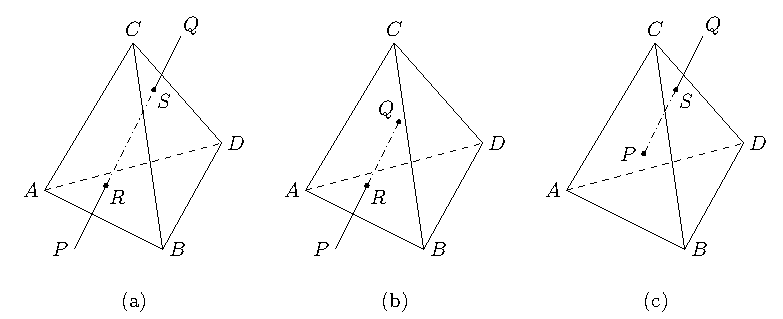
\includegraphics[width=1\textwidth]{figures/PQ}
\par\end{centering}
\caption{\label{fig:PQ}线段穿过四面体单元的几种常见情形}
\end{figure}


\subsection{求桨叶与体单元交集}

求线段 $\overline{PQ}$ 与四面体 $ABCD$ 的公共部分,可以归结为求线段 $\overline{PQ}$
与 $\triangle ABC$ 的公共点。设
\begin{equation}
\overline{PQ}=\lambda_{A}\overline{PA}+\lambda_{B}\overline{PB}+\lambda_{C}\overline{PC},
\end{equation}
即
\begin{equation}
\begin{bmatrix}(PQ)_{x}\\
(PQ)_{y}\\
(PQ)_{z}
\end{bmatrix}=\begin{bmatrix}(PA)_{x} & (PB)_{x} & (PC)_{x}\\
(PA)_{y} & (PB)_{y} & (PC)_{y}\\
(PA)_{z} & (PB)_{z} & (PC)_{z}
\end{bmatrix}\begin{bmatrix}\lambda_{A}\\
\lambda_{B}\\
\lambda_{C}
\end{bmatrix}\label{eq:segment_triangle_intersection}
\end{equation}

\begin{itemize}
\item 若点 $P$ 与 $\triangle ABC$ 不共面,即
\begin{equation}
\det\begin{bmatrix}(PA)_{x} & (PB)_{x} & (PC)_{x}\\
(PA)_{y} & (PB)_{y} & (PC)_{y}\\
(PA)_{z} & (PB)_{z} & (PC)_{z}
\end{bmatrix}\ne0,
\end{equation}
则关于 $\lambda_{A},\lambda_{B},\lambda_{C}$ 的方程 (\ref{eq:segment_triangle_intersection})
有唯一解。
\begin{itemize}
\item 若 $\lambda_{A},\lambda_{B},\lambda_{C}$ 均为正数,则直线 $PQ$ 与 $\triangle ABC$
有唯一的交点 $R$,且位于 $\triangle ABC$ 内部:
\begin{equation}
\overline{PR}=\frac{\overline{PQ}}{\lambda_{A}+\lambda_{B}+\lambda_{C}}
\end{equation}

\begin{itemize}
\item 若还有 $\lambda_{A}+\lambda_{B}+\lambda_{C}>1$,则点 $R$ 为线段 $\overline{PQ}$
与 $\triangle ABC$ 的交点,如图 \ref{fig:PQ} (a) 所示。
\item 否则,点 $R$ 位于线段 $\overline{PQ}$ 的延长线上,不是线段 $\overline{PQ}$ 与 $\triangle ABC$
的交点。
\end{itemize}
\item 否则,线段 $\overline{PQ}$ 与 $\triangle ABC$ 所属平面有唯一的交点,但不在 $\triangle ABC$
内。
\end{itemize}
\item 否则,判断点 $Q$ 是否与 $\triangle ABC$ 共面。
\begin{itemize}
\item 若点 $Q$ 与 $\triangle ABC$ 不共面,则点 $P$ 是直线 $PQ$ 与 $\triangle ABC$
所属平面的唯一交点。
\item 否则,直线 $PQ$ 与 $\triangle ABC$ 共面,但可能与 $\triangle ABC$ 没有公共点,需进一步讨论。
\end{itemize}
\end{itemize}


\section{间断、数值振荡与 WENO 重构技术\label{sec:WENO}}

双曲型方程(组)的广义解允许出现间断,按物理性质可以分为三类:
\begin{description}[wide]
\item [{激波}] 可以用厚度为零的控制体表示;物理量在其两侧的值有跳跃,因此是一种强间断;熵的值在其两侧有跳跃。一维激波的特征线呈汇聚状,如图
\ref{fig:shock} 所示。
\item [{膨胀波}] 可以用有限厚度的控制体表示;物理量在其内部光滑,在其边界两侧的值连续,但导数值有跳跃,因此是一种弱间断;熵的值在其两侧相等。一维膨胀波的特征线呈发散状,如图
\ref{fig:expansion} 所示。
\item [{接触间断}] 上述两种间断的临界情形:既可以看作熵变为零的激波,又可以看作厚度为零的膨胀波。一维接触间断的特征线相互平行,如图
\ref{fig:contact} 所示。
\end{description}

\begin{figure}[h!]
\begin{centering}
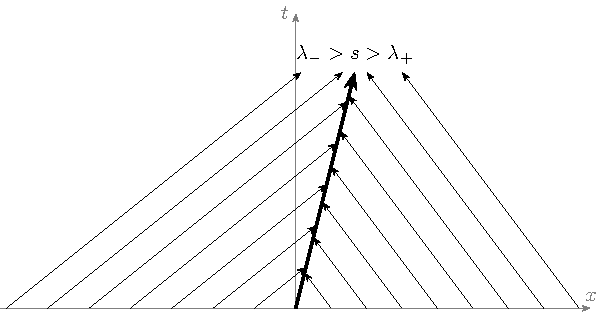
\includegraphics[width=1\textheight,height=0.26\textheight,keepaspectratio]{figures/shock}
\par\end{centering}
\caption{\label{fig:shock}一维激波的特征线呈汇聚状}
\end{figure}

直升机处于高速前飞状态时,主旋翼前行桨叶梢部的相对气流速度有可能超过当地声速,从而形成激波。直升机处于低速前飞或悬停状态时,主旋翼桨尖处的相对气流速度属于高亚声速,通常不会形成激波。无论是以上哪种情形,桨叶上下表面之间都存在有限的压强差。在
UMS–RKDG 近似解中,这是一种无法回避的间断,因为桨叶轴线一般会穿过 RKDG 格式所用的体单元。

\begin{figure}[h!]
\begin{centering}
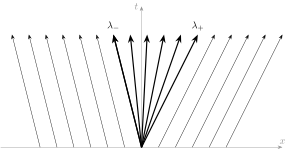
\includegraphics[width=1\textheight,height=0.26\textheight,keepaspectratio]{figures/expansion}
\par\end{centering}
\caption{\label{fig:expansion}一维膨胀波的特征线呈发散状}
\end{figure}

\begin{figure}[h!]
\begin{centering}
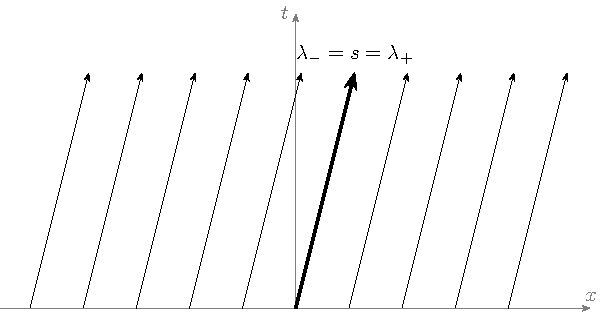
\includegraphics[width=1\textheight,height=0.26\textheight,keepaspectratio]{figures/contact}
\par\end{centering}
\caption{\label{fig:contact}一维接触间断的特征线相互平行}
\end{figure}

间断解的存在给高阶格式的设计带来了麻烦,这其中最致命的问题是存在于间断附近、幅值不随网格加密而衰减的“数值振荡 (numerical
oscillation)”。关于数值振荡的成因,学界存在多种观点,并有针对性地提出了多种压制策略:偏物理的解释有格式黏性不足、数值色散误差等观点,相应的策略包括人工黏性、群速度控制;偏数学的解释有格式单调性、吉布斯现象等,相应的策略有滤波器、限制器、高阶重构等。实际上,这些观点及策略在某种程度上是等价的。本文选用吉布斯现象\upcite{Gottlieb_1997}来解释数值振荡的成因,它是指:用有限项连续函数的线性组合
$u^{h}$ 对间断函数 $u$ 做近似,则连续函数 $u^{h}$ 在间断函数 $u$ 的间断处会发生数值振荡。图 \ref{fig:Gibbs}
展示了吉布斯现象的图象,以及数值振荡幅值不随网格加密而衰减的事实。

\begin{figure}[h!]
\begin{centering}
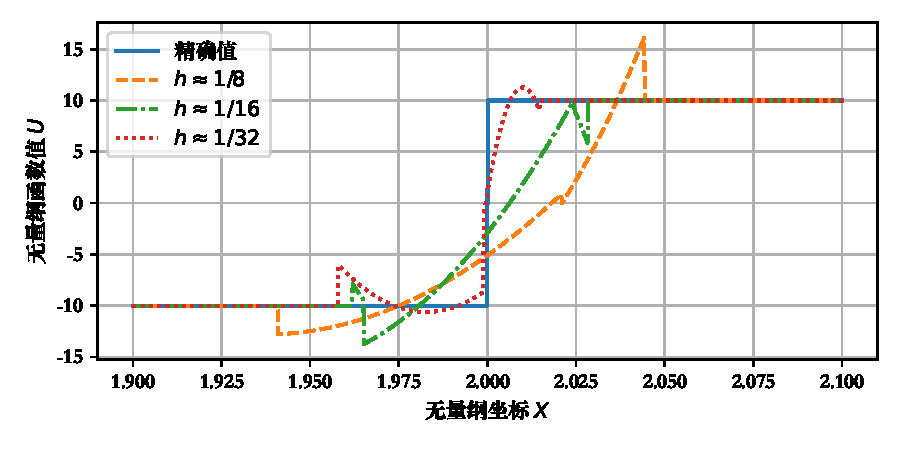
\includegraphics[width=1\textwidth]{figures/linear_scalar/gibbs}
\par\end{centering}
\caption{\label{fig:Gibbs}间断函数的 DG3 近似在间断附近发生数值振荡}
\end{figure}

高阶格式都必须以某种方式压制数值振荡。对于二阶有限差分格式,可以选用 Sweby 型限制器\upcite{Sweby_1984}。Van
Leer\upcite{Van_Leer_1977,Van_Leer_1977a,van_Leer_1979,van_Leer_2021}
提出的 MUSCL (monotonic upstream-centered scheme for conservation laws),被谨慎使用时可以达到三阶精度。这些方法一般不能直接应用于间断有限元格式,并且会在光滑极值点处降阶。

为了克服前一缺点(不适用于间断有限元),Cockburn\upcite{Cockburn_1990,Cockburn_1998} 提出了适用于高维问题的广义斜率限制器。这些
minmod 型限制器,结合具有 TVD 性质(或更一般的 SSP 性质)的 RK 格式,能够使高阶 DG 近似解不含非物理振荡,但往往会降低光滑区域极值点处的精度阶数。

为了克服后一缺点(在光滑极值点处降阶),Harten 等\upcite{Harten_1997}在有限差分法框架内提出了“基本无振荡
(essentially non-oscillatory, ENO\nomenclature[ENO]{ENO}{essentially non-oscillatory})”格式,其核心思想是:
\begin{itemize}
\item 为每个结点指定多个“候选模板 (candidate stencil)”。
\item 在每个候选模板上分别构造一个“候选多项式 (candidate polynomial)”。
\item 取“光滑程度 (smoothness)”最高的那一个作为近似解。
\end{itemize}

在近似解充分光滑的区域,各候选多项式的光滑程度通常也很接近,只保留其中一个显然是对计算资源的一种浪费。为了充分利用所有已知信息,“加权基本无振荡
(Weighted ENO, WENO\nomenclature{WENO}{weighted essentially non-oscillatory})”重构技术\upcite{Jiang_1996}将
ENO 格式的最后一步替换为:
\begin{itemize}
\item 取所有候选多项式的非线性加权平均作为近似解。
\end{itemize}

各种 WENO 重构技术的区别,正是体现在非线性权重的设计上。 ENO 格式与 WENO 重构技术虽不能完全消除数值振荡,但可以让数值振荡的幅值随网格加密而衰减,同时还能够避免近似解的精度在光滑极值点附近降阶,因此特别适合于既含间断(激波、接触间断、膨胀波)、又含复杂流动结构(湍流、涡系)的问题。

此后,WENO 重构技术被引入到高阶有限体积格式\upcite{Hu_1999}中,从而适用于非结构网格。类似的想法后来被移植到 RKDG
格式中\upcite{Qiu_2005,Zhu_2008},但代价是牺牲了 RKDG 格式的紧致性。适用于 RKDG 格式且保持其紧致特性的
WENO 重构技术\upcite{Zhong_2013,Zhu_2013,Mazaheri_2019},大约在 2013 年前后才开始出现,并且通常只给出二维版本的实现。

本节剩余部分将基于文献 \cite{Zhong_2013,Zhu_2013} 提出的二维 RKDG 格式的紧致型 WENO 限制器,提出一种适用于三维
RKDG 及 UMS–RKDG 格式的紧致型 WENO 限制器。

\subsection{适用于高阶差分格式的标量重构}

为求解一维标量守恒律
\begin{equation}
\frac{\partial u}{\partial t}+\frac{\partial f(u)}{\partial x}=0,\qquad a(u)=\frac{\partial f(u)}{\partial u},
\end{equation}
在等距网格上引入守恒型差分格式
\begin{equation}
\left(\partial_{x}f\right)_{i}\equiv\eval{\pdv{f}{x}}_{i}\approx\frac{f_{i+1/2}-f_{i-1/2}}{h},
\end{equation}
其中 $f_{i\pm1/2}$ 为下面将要构造的数值通量\nomenclature{$f_{i+1/2}$}{表示 $ x_{i+1/2} $ 处的数值通量}。不失一般性,这里只考虑
$a(u_{i})>0$ 的情形;对于 $a(u_{i})<0$ 的情形,只需将下标中紧跟在 $i$ 后面的 $\pm$ 互换,例如
$f_{i+1}$ 换为 $f_{i-1}$,以此类推。在构造 $f_{i+1/2}$ 时,含有五个点的大模板(用下标偏移量表示)
\begin{equation}
S=\begin{bmatrix}-2 & -1 & 0 & +1 & +2\end{bmatrix}
\end{equation}
被分解为三个各含三个点且部分重叠的小模板:
\begin{equation}
S_{1}=\begin{bmatrix}-2 & -1 & 0\end{bmatrix},\qquad S_{2}=\begin{bmatrix}-1 & 0 & +1\end{bmatrix},\qquad S_{3}=\begin{bmatrix}0 & +1 & +2\end{bmatrix}.
\end{equation}
由此可以构造出三种对 $\left(\partial_{x}f\right)_{i}$ 的三阶近似,相应的数值通量分别为\nomenclature{$f^{[k]}_{i+1/2}$}{表示在第 $k$ 号小模板上获得的 $ x_{i+1/2} $ 处的数值通量}
\begin{equation}
\begin{bmatrix}f_{i+1/2}^{[1]}\\
f_{i+1/2}^{[2]}\\
f_{i+1/2}^{[3]}
\end{bmatrix}=\frac{1}{6}\begin{bmatrix}2 & -7 & 11\\
 & -1 & 5 & 2\\
 &  & 2 & 5 & -1
\end{bmatrix}\begin{bmatrix}f_{i-2}\\
f_{i-1}\\
f_{i}\\
f_{i+1}\\
f_{i+2}
\end{bmatrix}.
\end{equation}
对三者取加权平均即得大模板上的数值通量:
\begin{equation}
f_{i+1/2}=\begin{bmatrix}w_{1} & w_{2} & w_{3}\end{bmatrix}\begin{bmatrix}f_{i+1/2}^{[1]}\\
f_{i+1/2}^{[2]}\\
f_{i+1/2}^{[3]}
\end{bmatrix},
\end{equation}
其中 $\begin{bmatrix}w_{1} & w_{2} & w_{3}\end{bmatrix}$ 是根据 $f$ 在
$\begin{bmatrix}S_{1} & S_{2} & S_{3}\end{bmatrix}$ 上的光滑程度构造的非线性权重\nomenclature{$w_k$}{表示第 $k$ 号小模板的非线性权重}:
\begin{itemize}
\item 在充分光滑的区域,上述 $f_{i+1/2}$ 应当逼近(五点)大模板上的(五阶)理想格式:
\begin{equation}
f_{i+1/2}^{S}=\frac{\begin{bmatrix}2 & -13 & 47 & 27 & -3\end{bmatrix}}{60}\begin{bmatrix}f_{i-2}\\
f_{i-1}\\
f_{i}\\
f_{i+1}\\
f_{i+2}
\end{bmatrix}.
\end{equation}
这可以通过取理想权重来实现\nomenclature{$w_k^{\star}$}{表示第 $k$ 号小模板的理想权重}:
\begin{equation}
\begin{bmatrix}w_{1} & w_{2} & w_{3}\end{bmatrix}=\begin{bmatrix}w_{1}^{\star} & w_{2}^{\star} & w_{3}^{\star}\end{bmatrix}\coloneqq\frac{1}{10}\begin{bmatrix}1 & 6 & 3\end{bmatrix}.
\end{equation}
\item 在非光滑区域,被间断穿过的小模板即“坏模板 (troubled stencil)”上的权重应当接近 $0$,但所有小模板的权重之和依然为
$1$。
\end{itemize}
文献 \cite{Jiang_1996} 给出了一种满足上述性质的方案:
\begin{enumerate}[wide]
\item 在小模板 $S_{k}$ 上构造二次多项式 $Q_{i}^{[k]}$ 作为在 $x_{i}$ 附近对 $f$ 的近似\nomenclature{$Q^{[k]}_{i}$}{表示在第 $k$ 号小模板构造的二次多项式近似}:
\begin{equation}
Q_{i}^{[k]}(x)=f_{i}+\eval{\pdv{f}{x}}_{i}^{[k]}(x-x_{i})+\eval{\pdv[2]{f}{x}}_{i}^{[k]}\frac{(x-x_{i})^{2}}{2},
\end{equation}
其中 $\left(\partial_{x}f\right)_{i}^{[k]}$ 与 $\left(\partial_{x}^{2}f\right)_{i}^{[k]}$
分别表示由 $\left\{ f_{i+s}:s\in S_{k}\right\} $ 给出的一阶与二阶差商,即 $\partial_{x}f$
与 $\partial_{x}^{2}f$ 在点 $x_{i}$ 处的近似值:
\begin{equation}
\begin{bmatrix}\left(\partial_{x}f\right)_{i}^{[1]}\\
\left(\partial_{x}f\right)_{i}^{[2]}\\
\left(\partial_{x}f\right)_{i}^{[3]}
\end{bmatrix}=\frac{1}{2h}\begin{bmatrix}1 & -4 & 3\\
 & -1 & 0 & 1\\
 &  & 3 & -4 & 1
\end{bmatrix}\begin{bmatrix}f_{i-2}\\
f_{i-1}\\
f_{i}\\
f_{i+1}\\
f_{i+2}
\end{bmatrix},
\end{equation}
\begin{equation}
\begin{bmatrix}\left(\partial_{x}^{2}f\right)_{i}^{[1]}\\
\left(\partial_{x}^{2}f\right)_{i}^{[2]}\\
\left(\partial_{x}^{2}f\right)_{i}^{[3]}
\end{bmatrix}=\frac{1}{h^{2}}\begin{bmatrix}1 & -2 & 1\\
 & 1 & -2 & 1\\
 &  & 1 & -2 & 1
\end{bmatrix}\begin{bmatrix}f_{i-2}\\
f_{i-1}\\
f_{i}\\
f_{i+1}\\
f_{i+2}
\end{bmatrix}.
\end{equation}
\item 计算二次多项式 $Q_{i}^{[k]}$ 在控制体 $(x_{i-1/2},x_{i+1/2})$ 上的光滑程度
\begin{equation}
\beta_{i}^{[k]}\coloneqq\int_{x_{i-1/2}}^{x_{i+1/2}}\sum_{p=1}^{2}\left(\dv[p]{Q_{i}^{[k]}}{x}\right)^{2}h^{2p-1}\dd{x}=\left(\eval{\pdv{f}{x}}_{i}^{[k]}h\right)^{2}+\frac{13}{12}\left(\eval{\pdv[2]{f}{x}}_{i}^{[k]}h^{2}\right)^{2}.
\end{equation}
在光滑区域,它们都趋于同一个二阶小量 $\beta_{i}^{\star}$,且两两之差为六阶小量:
\begin{equation}
\beta_{i}^{[k]}=\beta_{i}^{\star}+\order{h^{6}},\qquad\beta_{i}^{\star}\coloneqq\left(\eval{\pdv{f}{x}}_{i}h\right)^{2}+\frac{13}{12}\left(\eval{\pdv[2]{f}{x}}_{i}h^{2}\right)^{2}.
\end{equation}
在非光滑区域,坏模板上的 $Q_{i}^{[k]}$ 偏离 $f$ 在 $x_{i}$ 处的特例展开式较多,因此
\begin{equation}
\beta_{i}^{[k]}=\order{1}\gg\order{h^{2}}.
\end{equation}
\item 计算非线性权重
\begin{equation}
w_{k}=\frac{w_{k}^{\beta}}{w_{3}^{\beta}+w_{2}^{\beta}+w_{3}^{\beta}},\qquad w_{k}^{\beta}=\frac{w_{k}^{\star}}{\left(10^{-6}+\beta_{i}^{[k]}\right)^{2}}.
\end{equation}
在光滑区域,上述非线性权重接近理想权重:
\begin{equation}
w_{k}=w_{k}^{\star}+\order{h^{4}}\impliedby w_{k}^{\beta}=\frac{w_{k}^{\star}}{(\beta_{i}^{\star})^{2}+\order{h^{8}}}.
\end{equation}
故大模板上的 $f_{i+1/2}$ 具有五阶精度;在非光滑区域,坏模板的实际权重(与其他小模板的权重相比)接近 $0$,但大模板上的
$f_{i+1/2}$ 依然具有三阶精度。
\end{enumerate}


\subsection{适用于高阶 DG 格式的标量重构}

下面介绍由 Zhong\upcite{Zhong_2013} 提出(适用于结构网格)、并由 Zhu\upcite{Zhu_2013}
推广(适用于非结构网格)的适用于高阶 DG 格式的 WENO 重构方法。原文只给出了该方法的二维版本,本文将其适用范围推广到三维。

为方便叙述,将分片光滑的标量函数 $u$ 在体单元 $V_{i}$ 上的限制简记为\nomenclature{$u_{i}$}{表示标量函数 $u$ 在体单元 $V_{i}$ 上的限制}
\begin{equation}
u_{i}(\vec{r})\coloneqq u\vert_{V_{i}}(\vec{r}),\qquad\vec{r}\in V_{i},
\end{equation}
并将体单元 $V_{i}$ 及与之邻接的那些体单元的下标集(即局部模板)记为\nomenclature{$K_{i}$}{表示体单元 $V_{i}$ 及与之邻接的那些体单元的下标集(即局部模板)}
\begin{equation}
K_{i}\coloneqq\left\{ k:\partial V_{i}\cap\partial V_{k}\ne\varnothing\right\} .
\end{equation}
这里的“邻接”是指单元之间有公共边界,即几何区域相邻(三维单元至少有三个公共结点),而非单元编号相邻。

设 $u$ 为分段光滑的标量函数,通常为标量守恒律 $\partial_{t}u+\nabla\cdot\vec{f}=0$ 的多项式近似解,也可以是双曲型方程组的某个特征变量。对每个邻接单元,即
$\forall k\in K_{i}$:
\begin{itemize}
\item 将 $u_{k}$ 延拓到 $V_{i}$ 上,并对函数值做适当平移,\nomenclature{$u_{k\to i}$}{表示将标量函数 $u_{k}$ 延拓到 $V_{i}$ 上,并对函数值作适当平移(使其在 $V_{i}$ 上的均值等于 $u_{i}$ 在 $V_{i}$ 上的均值)所得的函数}使所得的
$u_{k\to i}$ 在 $V_{i}$ 上的均值等于 $u_{i}$ 在 $V_{i}$ 上的均值:
\begin{equation}
u_{k\to i}(\vec{r})\coloneqq u_{k}(\vec{r})-\langle u_{k}\rangle_{i}+\langle u_{i}\rangle_{i},\qquad\vec{r}\in V_{i},
\end{equation}
其中 $\langle u_{k}\rangle_{i}$ 表示函数 $u_{k}$ 在单元 $V_{i}$ 上的均值\nomenclature{$\langle u_{k}\rangle_{i}$}{表示标量函数 $u_{k}$ 在单元 $V_{i}$ 上的均值}:
\begin{equation}
\langle u_{k}\rangle_{i}\coloneqq\frac{\int_{V_{i}}u_{k}(\vec{r})}{\vert V_{i}\vert},\qquad\vert V_{i}\vert\coloneqq\int_{V_{i}}1.
\end{equation}
\item 为 $u_{k\to i}$ 分配理想权重:
\begin{equation}
w_{k\to i}^{\star}=\begin{cases}
0.001, & k\ne i,\\
1-\sum_{k\in K_{i}\setminus\left\{ i\right\} }w_{k\to i}^{\star}, & k=i,
\end{cases}
\end{equation}
其中 $w_{i\to i}^{\star}$ 为可调小量。数值试验表明:较大的 $w_{i\to i}^{\star}$ 有利于在光滑处保持精度,较小的
$w_{i\to i}^{\star}$ 有利于在间断处压制振荡。
\item 计算 $u_{k\to i}$ 在 $V_{i}$ 上的光滑程度\nomenclature{$\beta_{k\to i}$}{表示标量函数函数 $u_{k\to i}$ 在 $V_{i}$ 上的光滑程度}:
\begin{equation}
\beta_{k\to i}=\sum_{\vert\alpha\vert=1}^{p}\frac{\vert V_{i}\vert^{2\vert\alpha\vert/3-1}}{(\vert\alpha\vert!)^{2}}\int_{V_{i}}\left(\frac{\partial^{\vert\alpha\vert}u_{k\to i}}{\partial x^{\alpha_{x}}\partial y^{\alpha_{y}}\partial z^{\alpha_{z}}}\right)^{2},\qquad\vert\alpha\vert\coloneqq\alpha_{x}+\alpha_{y}+\alpha_{z},
\end{equation}
其中系数 $\vert V_{i}\vert^{2\vert\alpha\vert/3-1}/(\vert\alpha\vert!)^{2}$
的分子用于无量纲化,分母用于调节高阶导数的占比。文献 \cite{Zhu_2013} 中,此分子为 $\vert V_{i}\vert^{\vert\alpha\vert-1}$,其实是二维版本
$\vert V_{i}\vert^{2\vert\alpha\vert/2-1}$。
\item 计算非线性权重:
\begin{equation}
w_{k\to i}=\frac{w_{k\to i}^{\beta}}{\sum_{k\in K_{i}}w_{k\to i}^{\beta}},\qquad w_{k\to i}^{\beta}\coloneqq\frac{w_{k\to i}^{\star}}{\left(10^{-6}+\beta_{k\to i}\right)^{2}},
\end{equation}
其中 $10^{-6}$ 用于避免分母为零。
\end{itemize}

按上述非线性权重对 $\left\{ u_{k\to i}:k\in K_{i}\right\} $ 做平均,\nomenclature{$u_{i}^{\mathrm{new}}$}{表示 $u_{i}$ 经过 WENO 重构所得的新函数}以所得的新函数
$u_{i}^{\mathrm{new}}$ 取代旧函数 $u_{i}$:
\begin{equation}
u_{i}^{\mathrm{new}}(\vec{r})\coloneqq\sum_{k\in K_{i}}w_{k\to i}\,u_{k\to i}(\vec{r}),\qquad\vec{x}\in V_{i}.
\end{equation}


\subsection{适用于高阶 DG 格式的特征重构}

设多项式列阵 $\underline{U}$ 为双曲型方程组
\begin{equation}
\partial_{t}\underline{U}+\nabla\cdot\underline{\vec{F}}=\underline{H}\label{eq:hyperbolic_system}
\end{equation}
的广义解,将其在单元 $V_{i}$ 上的限制记为
\begin{equation}
\underline{U}_{i}(\vec{r},t)\coloneqq\underline{U}\vert_{V_{i}}(\vec{r},t),\qquad\vec{r}\in V_{i}.
\end{equation}
用 $\underline{U}_{i}^{h}$ 表示其近似解\nomenclature{$\underline{U}^{h}_{i}$}{表示双曲型方程组在单元 $V_i$ 上的近似解}\nomenclature{$\underline{U}^{h}$}{表示矩阵函数 $\underline{U}$ 在尺度为 $h$ 的网格上的多项式近似}。

遍历 $V_{i}$ 的邻居,即 $\forall k\in K_{i}\setminus\left\{ i\right\} $,将各邻接单元上的
$\underline{U}_{k}^{h}$ 延拓到 $V_{i}$ 上,并对函数值做适当平移,使所得的 $\underline{U}_{k\to i}^{h}$
在 $V_{i}$ 上的平均值等于 $\underline{U}_{i}^{h}$ 在 $V_{i}$ 上的平均值\nomenclature{$\underline{U}^{h}_{k\to i}$}{表示将矩阵函数 $\underline{U}^{h}_{k}$ 延拓到 $V_{i}$ 上,并对函数值作适当平移(使其在 $V_{i}$ 上的均值等于 $\underline{U}^{h}_{i}$ 在 $V_{i}$ 上的均值)所得的函数}:
\begin{equation}
\underline{U}_{k\to i}^{h}(\vec{r},t)\coloneqq\underline{U}_{k}^{h}(\vec{r},t)-\langle\underline{U}_{k}^{h}\rangle_{i}+\langle\underline{U}_{i}^{h}\rangle_{i},\qquad\vec{r}\in V_{i}.
\end{equation}
不难证明:$\underline{U}_{i}^{h}$ 在 $V_{i}$ 上的平均值是重构不变量,即
\begin{equation}
\langle\underline{U}_{k\to i}^{h}\rangle_{i}=\langle\underline{U}_{i}^{h}\rangle_{i}.
\end{equation}

再次遍历 $V_{i}$ 的邻居,即 $\forall k\in K_{i}\setminus\left\{ i\right\} $,对方程组
(\ref{eq:hyperbolic_system}) 沿公共边界 $\partial V_{i}\cap\partial V_{k}$
的\nomenclature{$\vec{\nu}_{k}$}{表示体单元 $V_{i}$ 与 $V_{k}$ 的公共边界 $\partial V_{i}\cap\partial V_{k}$ 上的单位法向量}法向量
$\vec{\nu}_{k}$ 的法向分裂形式\nomenclature{$\underline{F}^{\nu_{k}}$}{表示  $\underline{\vec{F}}$ 在 $\vec{\nu}_{k}$ 上投影所得的法向通量}\nomenclature{$\underline{A}^{\nu_{k}}$}{表示  $\underline{F}^{\nu_{k}}$ 关于 $\underline{U}$ 的雅可比矩阵}
\begin{equation}
\partial_{t}\underline{U}+\partial_{\nu_{k}}\underline{F}^{\nu_{k}}=\underline{H},\qquad\underline{F}^{\nu_{k}}\coloneqq\vec{\nu}_{k}\cdot\vec{\underline{F}},\qquad\underline{A}^{\nu_{k}}\coloneqq\partial\underline{F}^{\nu_{k}}/\partial\underline{U},
\end{equation}
实施如下特征重构:
\begin{itemize}
\item 用重构不变量 $\langle\underline{U}_{i}^{h}\rangle_{i}$,即 $\underline{U}_{i}^{h}$
在 $V_{i}$ 上的均值,计算 $\underline{A}^{\nu_{k}}(\underline{U}_{i})$ 所得的近似值\nomenclature{$\underline{A}_{i\vert k}$}{表示用 $\underline{U}^{h}_{i}$ 在 $V_{i}$ 上的均值计算 $\underline{A}^{\nu_{k}}(\underline{U}_{i})$ 所得的近似值}:
\begin{equation}
\underline{A}^{\nu_{k}}(\underline{U})\approx\underline{A}^{\nu_{k}}\qty(\langle\underline{U}_{i}^{h}\rangle_{i})\eqqcolon\underline{A}_{i\vert k}.
\end{equation}
下标里的 $i\vert k$ 表示它是在 $V_{k}$ 的帮助下得到的属于 $V_{i}$ 的结果(下同)。
\item 对所得的 $\underline{A}_{i\vert k}$ 做特征分解\nomenclature{$\underline{R}_{i\vert k}$}{表示 $\underline{A}_{i\vert k}$ 的右特征矩阵}\nomenclature{$\underline{L}_{i\vert k}$}{表示 $\underline{A}_{i\vert k}$ 的左特征矩阵}:
\begin{equation}
\underline{A}_{i\vert k}\,\underline{R}_{i\vert k}=\underline{R}_{i\vert k}\,\underline{\varLambda}_{i\vert k},\qquad\underline{L}_{i\vert k}\coloneqq(\underline{R}_{i\vert k})^{-1}.\label{eq:eigen-decomposition}
\end{equation}
\item 用左特征矩阵 $\underline{L}_{i\vert k}$ 定义特征变量\nomenclature{$\underline{W}_{i\vert k}$}{表示利用 $\underline{L}_{i\vert k}$ 构造的特征变量}:
\begin{equation}
\underline{W}_{i\vert k}\coloneqq\underline{L}_{i\vert k}\,\underline{U}.
\end{equation}
将 $\underline{U}_{k\to i}^{h}$ 代入右端,得到 $\underline{W}_{i\vert k}$
的近似值,记为 $\underline{W}_{i\vert k}^{h}$。该近似值可能含有数值振荡。
\item 将 $\underline{W}_{i\vert k}$ 的每一行视为独立变量,对其调用标量重构算法,用 $\underline{W}_{i\vert k}^{h,\mathrm{new}}$
表示重构后的、基本无振荡的特征变量近似值。\nomenclature{$\underline{W}_{i\vert k}^{h,\mathrm{new}}$}{表示 $\underline{W}^h_{i\vert k}$ 经过 WENO 重构所得的新函数}
\item 用右特征矩阵 $\underline{R}_{i\vert k}$ 将其变换回守恒变量:
\begin{equation}
\underline{U}_{i\vert k}^{h,\mathrm{new}}\coloneqq\underline{R}_{i\vert k}\,\underline{W}_{i\vert k}^{h,\mathrm{new}}.
\end{equation}
\item 最后按单元 $V_{k}$ 的体积对 $\underline{U}_{i\vert k}^{h,\mathrm{new}}$ 作加权平均:
\begin{equation}
\underline{U}_{i}^{h,\mathrm{new}}\coloneqq\frac{\sum_{k\in K_{i}\setminus\left\{ i\right\} }\vert V_{k}\vert\,\underline{U}_{i\vert k}^{h,\mathrm{new}}}{\sum_{k\in K_{i}\setminus\left\{ i\right\} }\vert V_{k}\vert}
\end{equation}
以此作为 $\underline{U}_{i}$ 的新近似解。\nomenclature{$\underline{U}^{h,\mathrm{new}}_{i}$}{表示 $\underline{U}^h_{i}$ 经过 WENO 重构所得的新函数}
\end{itemize}

上述过程在每个公共边界 $\partial V_{i}\cap\partial V_{k}$ 上只做一次法向投影,实际上是假设了单位法向量
$\vec{\nu}_{k}$ 沿该边界不变,即单元边界属于某个平面\footnote{在三维问题中,四面体单元通常可以保证不属于任何平面的单元边界只出现在流场边界上,而六面体单元(即使最低阶的八结点单元)的单元边界一般而言是非平面的。}。

\subsection{三维欧拉方程的特征分解}

以上特征重构方法原则上适用于任意双曲型方程。对于本文最关心的三维欧拉方程,式 (\ref{eq:eigen-decomposition})
所示特征分解可以通过符号运算提前做好。本节给出该结果的推导过程。

三维欧拉方程的法向分裂形式\nomenclature{$\rho$}{表示气体密度}\nomenclature{$p$}{表示气体压强}\nomenclature{$e_0$}{表示气体比总能}\nomenclature{$h_0$}{表示气体比总焓}\nomenclature{$\vec{u}$}{表示气体速度}
\begin{equation}
\frac{\partial}{\partial t}\begin{bmatrix}\rho\\
\rho\vec{u}\\
\rho e_{0}
\end{bmatrix}+\frac{\partial}{\partial\nu}\begin{bmatrix}\rho u_{\nu}\\
\rho u_{\nu}\vec{u}+p\vec{\nu}\\
\rho u_{\nu}h_{0}
\end{bmatrix}=\begin{bmatrix}0\\
\vec{0}\\
0
\end{bmatrix}
\end{equation}
在全局 $(x,y,z)$ 坐标系下的展开式为
\begin{equation}
\frac{\partial}{\partial t}\begin{bmatrix}\rho\\
\rho u_{x}\\
\rho u_{y}\\
\rho u_{z}\\
\rho e_{0}
\end{bmatrix}+\frac{\partial}{\partial\nu}\begin{bmatrix}\rho u_{\nu}\\
\rho u_{\nu}u_{x}+p\nu_{x}\\
\rho u_{\nu}u_{y}+p\nu_{y}\\
\rho u_{\nu}u_{z}+p\nu_{z}\\
\rho u_{\nu}h_{0}
\end{bmatrix}=\begin{bmatrix}0\\
0\\
0\\
0\\
0
\end{bmatrix},
\end{equation}
在局部 $(\nu,\sigma,\pi)$ 坐标系下的展开式为
\begin{equation}
\frac{\partial}{\partial t}\begin{bmatrix}\rho\\
\rho u_{\nu}\\
\rho u_{\sigma}\\
\rho u_{\pi}\\
\rho e_{0}
\end{bmatrix}+\frac{\partial}{\partial\nu}\begin{bmatrix}\rho u_{\nu}\\
\rho u_{\nu}u_{\nu}+p\\
\rho u_{\nu}u_{\sigma}\\
\rho u_{\nu}u_{\pi}\\
\rho u_{\nu}h_{0}
\end{bmatrix}=\begin{bmatrix}0\\
0\\
0\\
0\\
0
\end{bmatrix}.
\end{equation}
后者的特征值为
\begin{equation}
\underline{\varLambda'}=\begin{bmatrix}u_{\nu}-a\\
 & u_{\nu}\\
 &  & u_{\nu}\\
 &  &  & u_{\nu}\\
 &  &  &  & u_{\nu}+a
\end{bmatrix},
\end{equation}
相应的右特征矩阵\nomenclature{$\underline{R'}$}{表示 $\underline{A}^{\nu}$ 的右特征矩阵在法向坐标系中的表达式}为
\begin{equation}
\underline{R'}=\begin{bmatrix}1 & 1 & 0 & 0 & 1\\
u_{\nu}-a & u_{\nu} & 0 & 0 & u_{\nu}+a\\
u_{\sigma} & u_{\sigma} & 1 & 0 & u_{\sigma}\\
u_{\pi} & u_{\pi} & 0 & 1 & u_{\pi}\\
h_{0}-u_{\nu}a & \frac{u_{\nu}^{2}+u_{\sigma}^{2}+u_{\pi}^{2}}{2} & u_{\sigma} & u_{\pi} & h_{0}+u_{\nu}a
\end{bmatrix}.
\end{equation}
利用符号运算可得左特征矩阵\nomenclature{$\underline{L'}$}{表示 $\underline{A}^{\nu}$ 的左特征矩阵在法向坐标系中的表达式}:
\begin{equation}
\underline{L'}=(\underline{R'})^{-1}=\begin{bmatrix}\frac{1}{2}\left(B_{2}+u_{\nu}/a\right) & -\frac{1}{2}\left(B_{1}u_{\nu}+1/a\right) & -\frac{1}{2}B_{1}u_{\sigma} & -\frac{1}{2}B_{1}u_{\pi} & \frac{1}{2}B_{1}\\
1-B_{2} & B_{1}u_{\nu} & B_{1}u_{\sigma} & B_{1}u_{\pi} & -B_{1}\\
-u_{\sigma} & 0 & 1 & 0 & 0\\
-u_{\pi} & 0 & 0 & 1 & 0\\
\frac{1}{2}\left(B_{2}-u_{\nu}/a\right) & -\frac{1}{2}\left(B_{1}u_{\nu}-1/a\right) & -\frac{1}{2}B_{1}u_{\sigma} & -\frac{1}{2}B_{1}u_{\pi} & \frac{1}{2}B_{1}
\end{bmatrix},
\end{equation}
其中
\begin{equation}
B_{1}\coloneqq\frac{\gamma^{-}}{a^{2}},\qquad B_{2}\coloneqq B_{1}\frac{u_{\nu}^{2}+u_{\sigma}^{2}+u_{\pi}^{2}}{2}.
\end{equation}

利用变量替换关系
\begin{equation}
\underline{U}=\underline{J}_{\underline{U}\to\underline{U'}}\,\underline{U'}
\end{equation}
即
\begin{equation}
\begin{bmatrix}\rho\\
\rho u_{x}\\
\rho u_{y}\\
\rho u_{z}\\
\rho e_{0}
\end{bmatrix}=\begin{bmatrix}\rho\\
\rho u_{\nu}\nu_{x}+\rho u_{\sigma}\sigma_{x}+\rho u_{\pi}\pi_{x}\\
\rho u_{\nu}\nu_{y}+\rho u_{\sigma}\sigma_{y}+\rho u_{\pi}\pi_{y}\\
\rho u_{\nu}\nu_{z}+\rho u_{\sigma}\sigma_{z}+\rho u_{\pi}\pi_{z}\\
\rho e_{0}
\end{bmatrix}=\begin{bmatrix}1\\
 & \nu_{x} & \sigma_{x} & \pi_{x}\\
 & \nu_{y} & \sigma_{y} & \pi_{y}\\
 & \nu_{z} & \sigma_{z} & \pi_{z}\\
 &  &  &  & 1
\end{bmatrix}\begin{bmatrix}\rho\\
\rho u_{\nu}\\
\rho u_{\sigma}\\
\rho u_{\pi}\\
\rho e_{0}
\end{bmatrix}
\end{equation}
可得右特征矩阵在全局 $(x,y,z)$ 坐标系下的表达式\nomenclature{$\underline{R}$}{表示 $\underline{A}^{\nu}$ 的右特征矩阵在全局坐标系中的表达式}:
\begin{equation}
\underline{R}=\underline{J}_{\underline{U}\to\underline{U'}}\,\underline{R'}=\begin{bmatrix}1 & 1 & 0 & 0 & 1\\
u_{x}-a\nu_{x} & u_{x} & \sigma_{x} & \pi_{x} & u_{x}+a\nu_{x}\\
u_{y}-a\nu_{y} & u_{y} & \sigma_{y} & \pi_{y} & u_{y}+a\nu_{y}\\
u_{z}-a\nu_{z} & u_{z} & \sigma_{z} & \pi_{z} & u_{z}+a\nu_{z}\\
h_{0}-u_{\nu}a & \frac{u_{x}^{2}+u_{y}^{2}+u_{z}^{2}}{2} & u_{\sigma} & u_{\pi} & h_{0}+u_{\nu}a
\end{bmatrix},
\end{equation}
这里用
\begin{equation}
\begin{bmatrix}u_{\nu}\\
u_{\sigma}\\
u_{\pi}
\end{bmatrix}=\begin{bmatrix}\nu_{x} & \sigma_{x} & \pi_{x}\\
\nu_{y} & \sigma_{y} & \pi_{y}\\
\nu_{z} & \sigma_{z} & \pi_{z}
\end{bmatrix}^{-1}\begin{bmatrix}u_{x}\\
u_{y}\\
u_{z}
\end{bmatrix}
\end{equation}
对速度分量做了替换。

\newpage{}

同理,可得左特征矩阵在全局 $(x,y,z)$ 坐标系下的表达式\nomenclature{$\underline{L}$}{表示 $\underline{A}^{\nu}$ 的左特征矩阵在全局坐标系中的表达式}:
\begin{equation}
\begin{aligned}\underline{L} & =\underline{L'}\,\underline{J}_{\underline{U}\to\underline{U'}}^{-1}\\
 & =\begin{bmatrix}\frac{1}{2}\left(B_{2}+u_{\nu}/a\right) & 1-B_{2} & -u_{\sigma} & -u_{\pi} & \frac{1}{2}\left(B_{2}-u_{\nu}/a\right)\\
-\frac{1}{2}\left(B_{1}u_{x}+\nu_{x}/a\right) & B_{1}u_{x} & \sigma_{x} & \pi_{x} & -\frac{1}{2}\left(B_{1}u_{x}-\nu_{x}/a\right)\\
-\frac{1}{2}\left(B_{1}u_{y}+\nu_{y}/a\right) & B_{1}u_{y} & \sigma_{y} & \pi_{y} & -\frac{1}{2}\left(B_{1}u_{y}-\nu_{y}/a\right)\\
-\frac{1}{2}\left(B_{1}u_{z}+\nu_{z}/a\right) & B_{1}u_{z} & \sigma_{z} & \pi_{z} & -\frac{1}{2}\left(B_{1}u_{z}-\nu_{z}/a\right)\\
\frac{1}{2}B_{1} & -B_{1} & 0 & 0 & \frac{1}{2}B_{1}
\end{bmatrix}^{t}
\end{aligned}
\end{equation}


\section{本章小结}

本章提出了一种适用于舰载直升机流场的高阶计算方法。该方法具有以下优点:
\begin{description}[wide]
\item [{能够处理几何外形复杂的边界}] 该方法用间断伽辽金 (DG) 格式做空间离散,能够在三维非结构网格上的构造紧致的高阶格式,既克服了有限差分格式仅适用于结构网格的弊端,又解决了高阶有限差分格式局部模板过宽的问题。对于舰载直升机三维流场计算,这种优势能够让高阶计算格式很好地适应复杂的船体外形及直升机机身外形。
\item [{能够保持数值解的强稳定性}] 该方法以保持强稳定性的显式 Runge–Kutta (RK) 格式做时间推进,能够像显式欧拉格式那样给出物理上可靠的结果。除此之外,显式
$p$ 阶 RK 格式避免了大型代数方程组的生成与求解,简化了程序实现,与紧致的 $q$ 阶 DG 格式相互配合,保证了整个 RK$p$/DG$q$
格式具有高度的可并行性。为明确区分时间离散与空间离散的阶数,这里及本文剩余部分把用 $p$ 阶 (SSP) RK 格式做时间推进、用
$q$ 阶 DG 有限元法做空间离散的具体格式称为“RK$p$/DG$q$ 格式”,并称基于该格式的求解器、近似解为“RK$p$/DG$q$
求解器、近似解”;称构造这些格式的方法为“RKDG 方法”。若时空精度皆为 $p$,则“RK$p$/DG$q$”(格式、求解器、近似解)也可简称为“$p$
阶 RKDG”(格式、求解器、近似解)。\nomenclature{RKDG}{Runge--Kutta discontinuous Galerkin}\nomenclature{RK$p$/DG$q$}{$p$th order Runge–Kutta and $q$th order discontinuous Galerkin}
\item [{避免了对动态网格技术的依赖}] 该方法以非定常动量源 (UMS) 模型表示桨叶对流场的扰动,避免了旋翼 CFD 对变形网格、滑动网格、重叠网格等动态网格技术的依赖,大大降低了程序实现的难度。该模型与高阶
RKDG 格式相结合,能够在较为粗糙的三维非结构网格上,高效(相对于动态网格技术)且高精度(相对于经典有限体积)捕获旋翼流场的非定常特征。
\item [{压制了高阶近似解的数值振荡}] 该方法以紧致型 WENO 重构技术,压制高阶 RKDG 及高阶 UMS–RKDG 近似解在间断附近的数值振荡。本文所借鉴的二维
WENO 重构技术,原本被用于压制高阶 RKDG 近似解在激波、接触间断、膨胀波边界附近的数值振荡。尽管对常规直升机而言,只有在高速飞行时才会在前行桨叶梢部形成激波;但
UMS 模型的引入,使得被桨叶穿过的体单元内部始终存在压强间断。因此,要获得正确的高阶 UMS–RKDG 近似解,必须开启本章所给出的三维
WENO 限制器。
\end{description}


\chapter{高阶格式在非结构网格上的精度验证\label{chap:=009A8C=008BC1}}

本章首先基于一组具有解析解或数值精确解的一维标准算例,在三维非结构网格上定量验证第\ref{chap:=007B97=006CD5}章所提高阶计算方法的正确性,以及提高阶数对减小误差所起的作用。在此基础上,基于一组没有解析解、数值精确解,但有高精度数值精的二维标准算例,在三维非结构网格上定性验证高阶格式的正确性及高精度。

\section{基于线性平流问题解析解的定量验证}

本节求解如下线性平流方程
\begin{equation}
\partial_{t}\underline{U}+\underline{A}^{x}\,\partial_{x}\underline{U}+\underline{A}^{y}\,\partial_{y}\underline{U}+\underline{A}^{z}\,\partial_{z}\underline{U}=\underline{0}\label{eq:linear_system}
\end{equation}
的初边值问题。这组问题的解析解可以由文献 \cite{Toro_2009} 介绍的方法获得,因而很适合被用于数值求解器性能的定量评估。本节所有问题都是在三维区间
$[0,4]\times[0,1]\times[0,0.5]$ 内求解的,且所有平行于 $x$ 轴的边界均以“法向导数为零”为边界条件,即
\begin{equation}
\partial_{\nu}\underline{U}=\underline{0},\qquad(y-0)(y-1)(z-0)(z-0.5)=0.
\end{equation}


\subsection{线性单波平流问题}
\begin{problem}
[线性单波平流]\label{prob:=007EBF=006027=005355=006CE2=005E73=006D41}在方程
(\ref{eq:linear_system}) 中,令
\begin{equation}
\underline{U}(x,y,z,t)=\begin{bmatrix}U(x,y,z,t)\end{bmatrix},\qquad\underline{A}^{x}=\begin{bmatrix}-10\end{bmatrix},\qquad\underline{A}^{y}=\underline{A}^{z}=\begin{bmatrix}0\end{bmatrix},
\end{equation}
即得线性单波方程
\begin{equation}
\left(\partial_{t}-10\partial_{x}\right)U=0.
\end{equation}
求满足此方程与边界条件
\begin{equation}
U(x=0,y,z,t)=-10\eqqcolon U_{\mathrm{L}},\qquad U(x=4,y,z,t)=+10\eqqcolon U_{\mathrm{R}},
\end{equation}
及初始条件
\begin{equation}
U(x,y,z,t=0)=U_{\mathrm{L}}
\end{equation}
的广义解。
\end{problem}

该问题的解析解为
\begin{equation}
U^{\star}(x,y,z,t)=\begin{cases}
U_{\mathrm{L}}, & x-4<-10t;\\
U_{\mathrm{R}}, & x-4>-10t.
\end{cases}
\end{equation}
其物理意义为以速率 $10$ 沿 $-x$ 方向移动的平面波。初始时,长方体内部为均匀状态,但有一间断位于 $x=4$ 处。

为了直观地比较数值解的精度,图 \ref{fig:linear_scalar_contour} 给出了若干求解器–网格 ($p$–$h$)
组合给出的同一时刻的数值解云图。这些图中的白色区域为函数值连续变化的过渡层,其厚度与数值解的误差呈正相关。通过比较图 \ref{subfig:linear_scalar_p=00003D1_h=00003D2^-5}
所示的细 ($h\approx1/32$) 网格上的低阶 ($p=1$) 数值解,与图 \ref{subfig:linear_scalar_p=00003D3_h=00003D2^-2}
所示粗 ($h\approx1/4$) 网格上的高阶 ($p=3$) 数值解,可知二者的误差在同一量级。

\begin{figure}[h!]
\begin{centering}
\subfloat[\label{subfig:linear_scalar_p=00003D3_h=00003D2^-3}时空精度 $p=3$,网格尺度
$h\approx2^{-3}$]{\begin{centering}
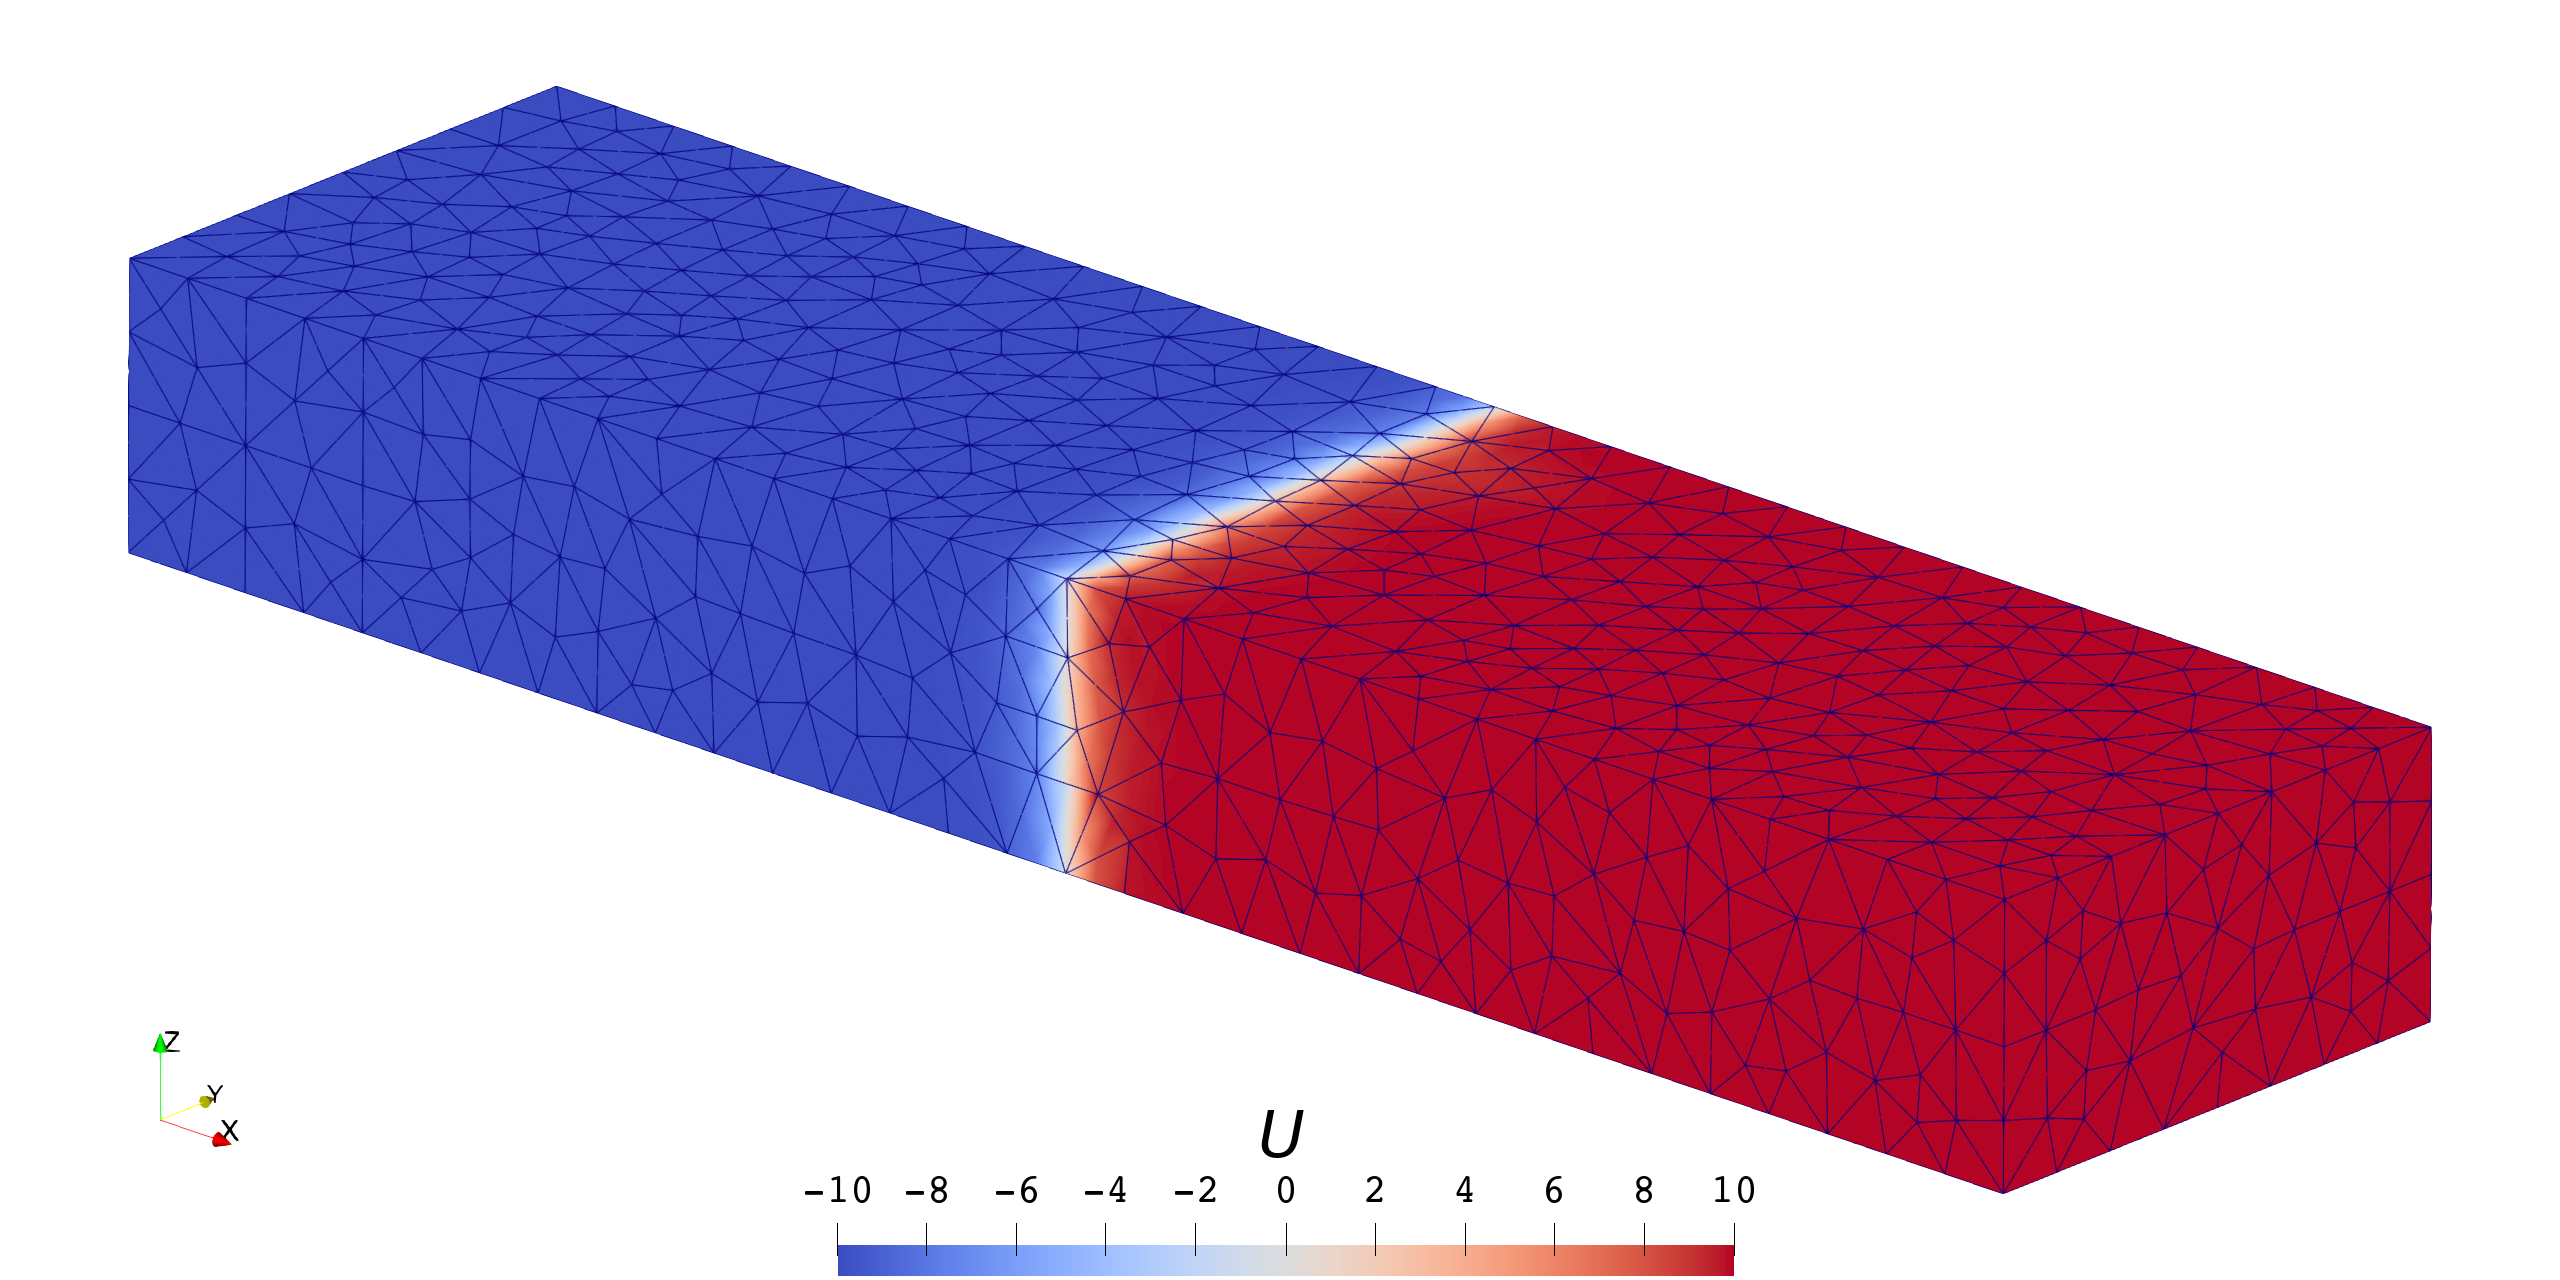
\includegraphics[width=1\textwidth,height=0.4\textheight,keepaspectratio]{../mdpi/figures/linear_scalar/p=3_h=2^-3}
\par\end{centering}
}
\par\end{centering}
\begin{centering}
\subfloat[\label{subfig:linear_scalar_p=00003D1_h=00003D2^-5}时空精度 $p=1$,网格尺度
$h\approx2^{-5}$]{\begin{centering}
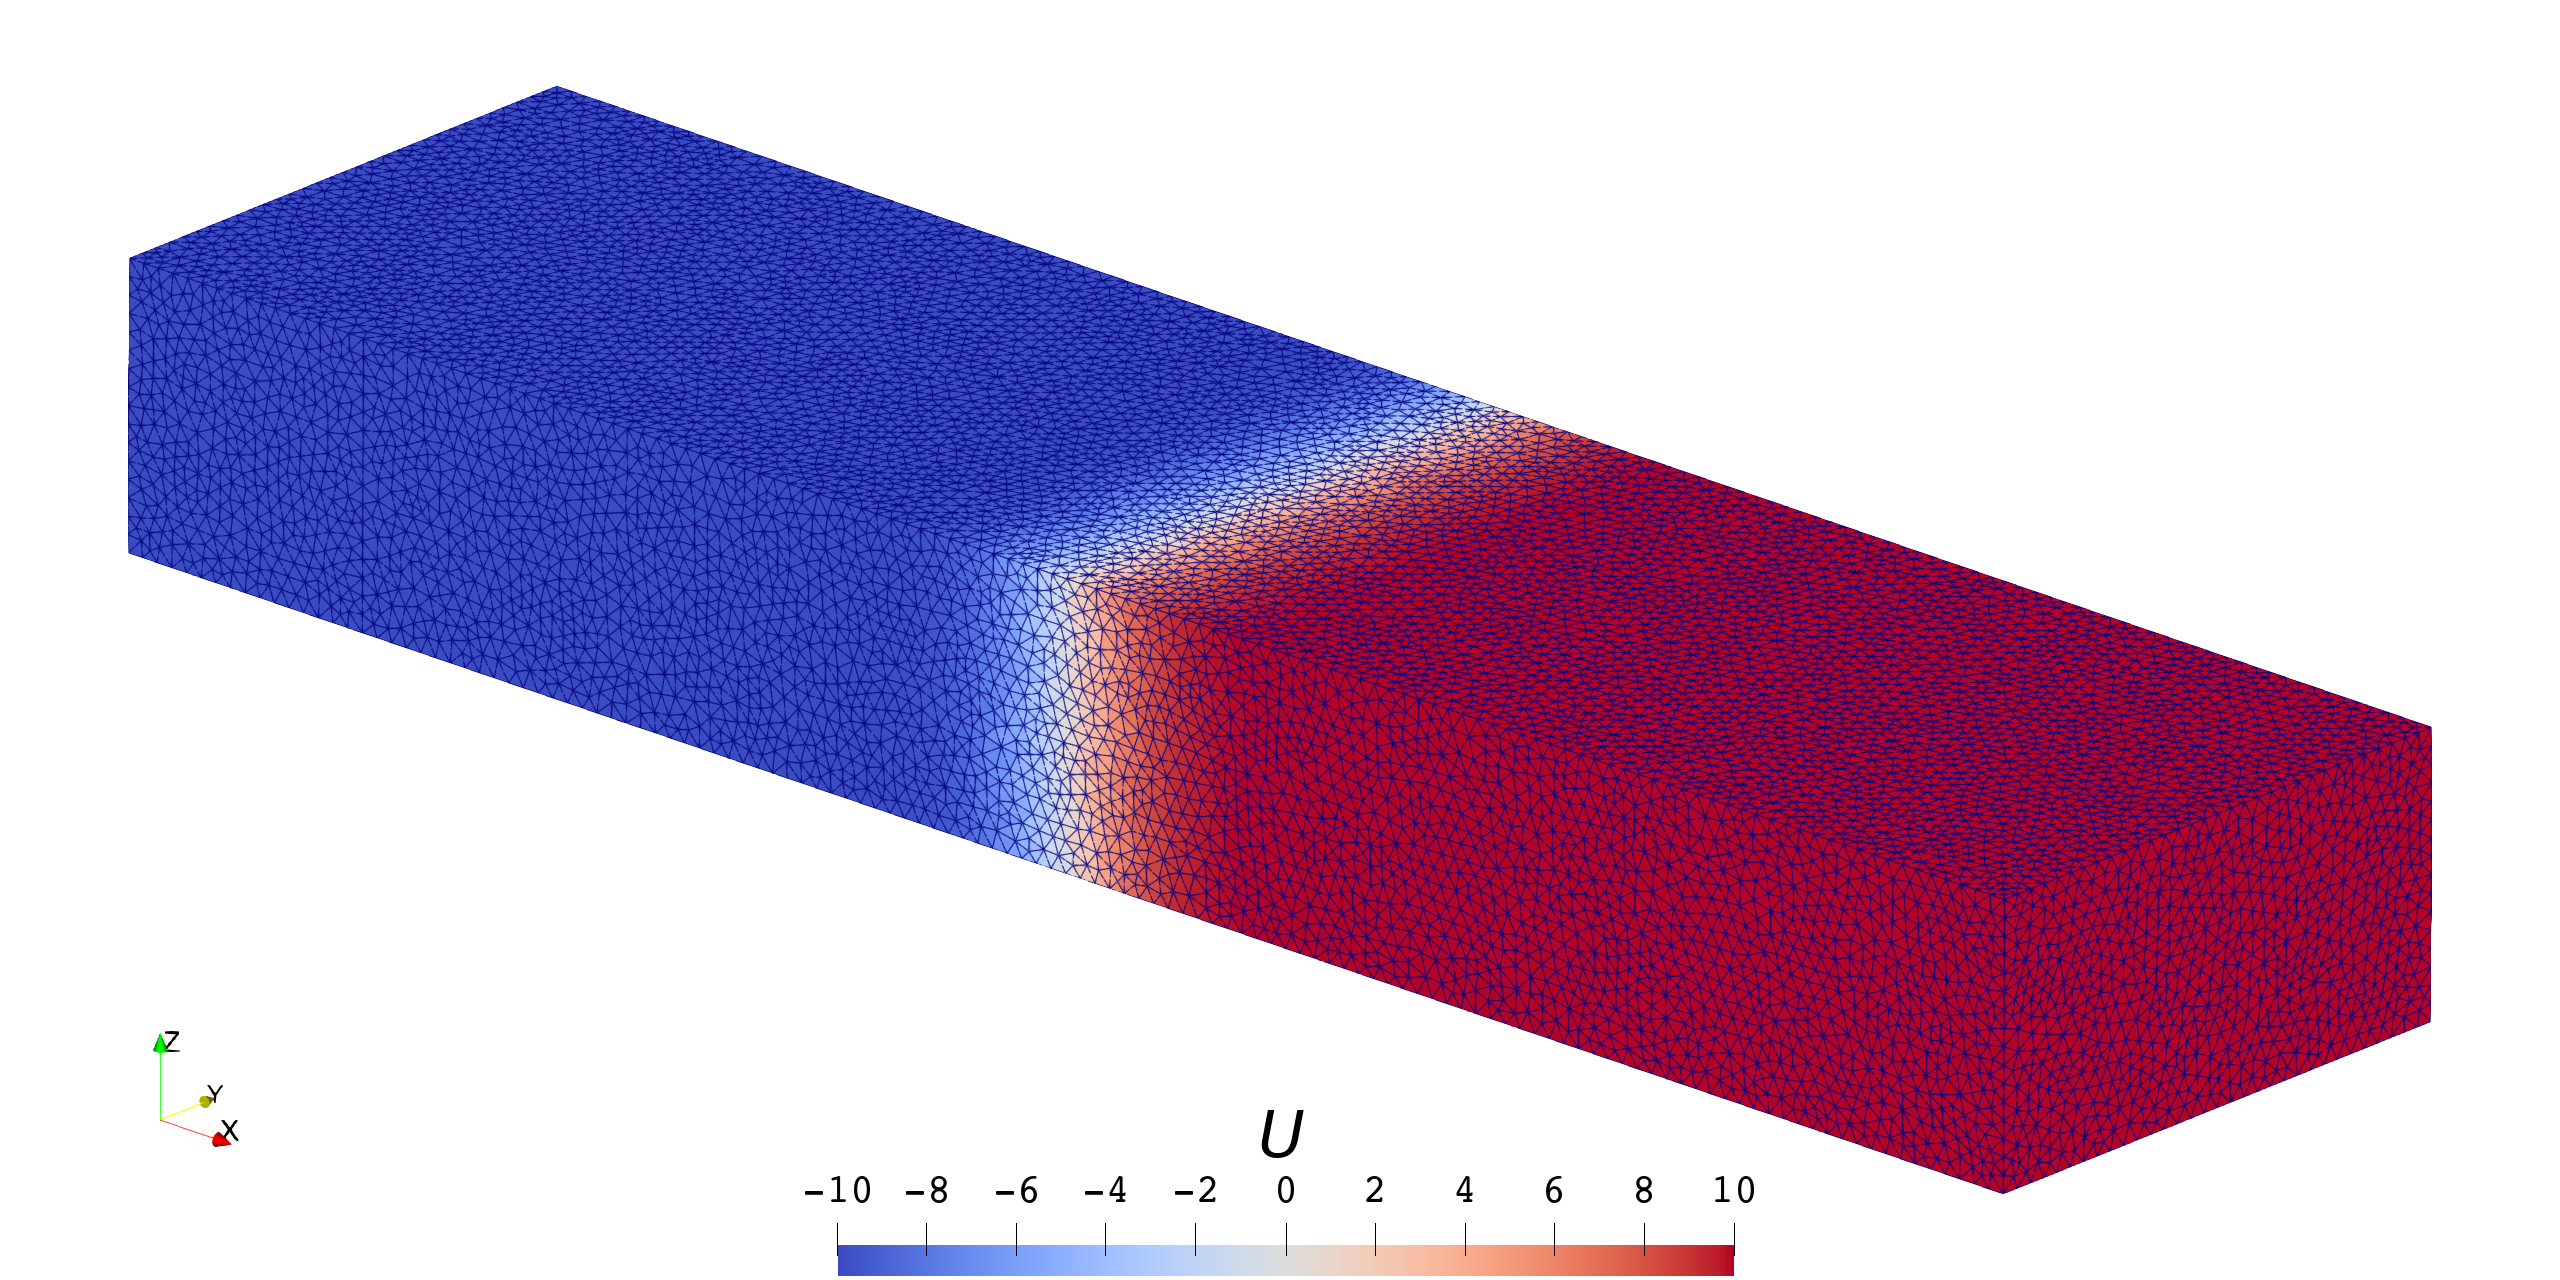
\includegraphics[width=1\textwidth,height=0.4\textheight,keepaspectratio]{../mdpi/figures/linear_scalar/p=1_h=2^-5}
\par\end{centering}
}
\par\end{centering}
\begin{centering}
\subfloat[\label{subfig:linear_scalar_p=00003D3_h=00003D2^-2}时空精度 $p=3$,网格尺度
$h\approx2^{-2}$]{\begin{centering}
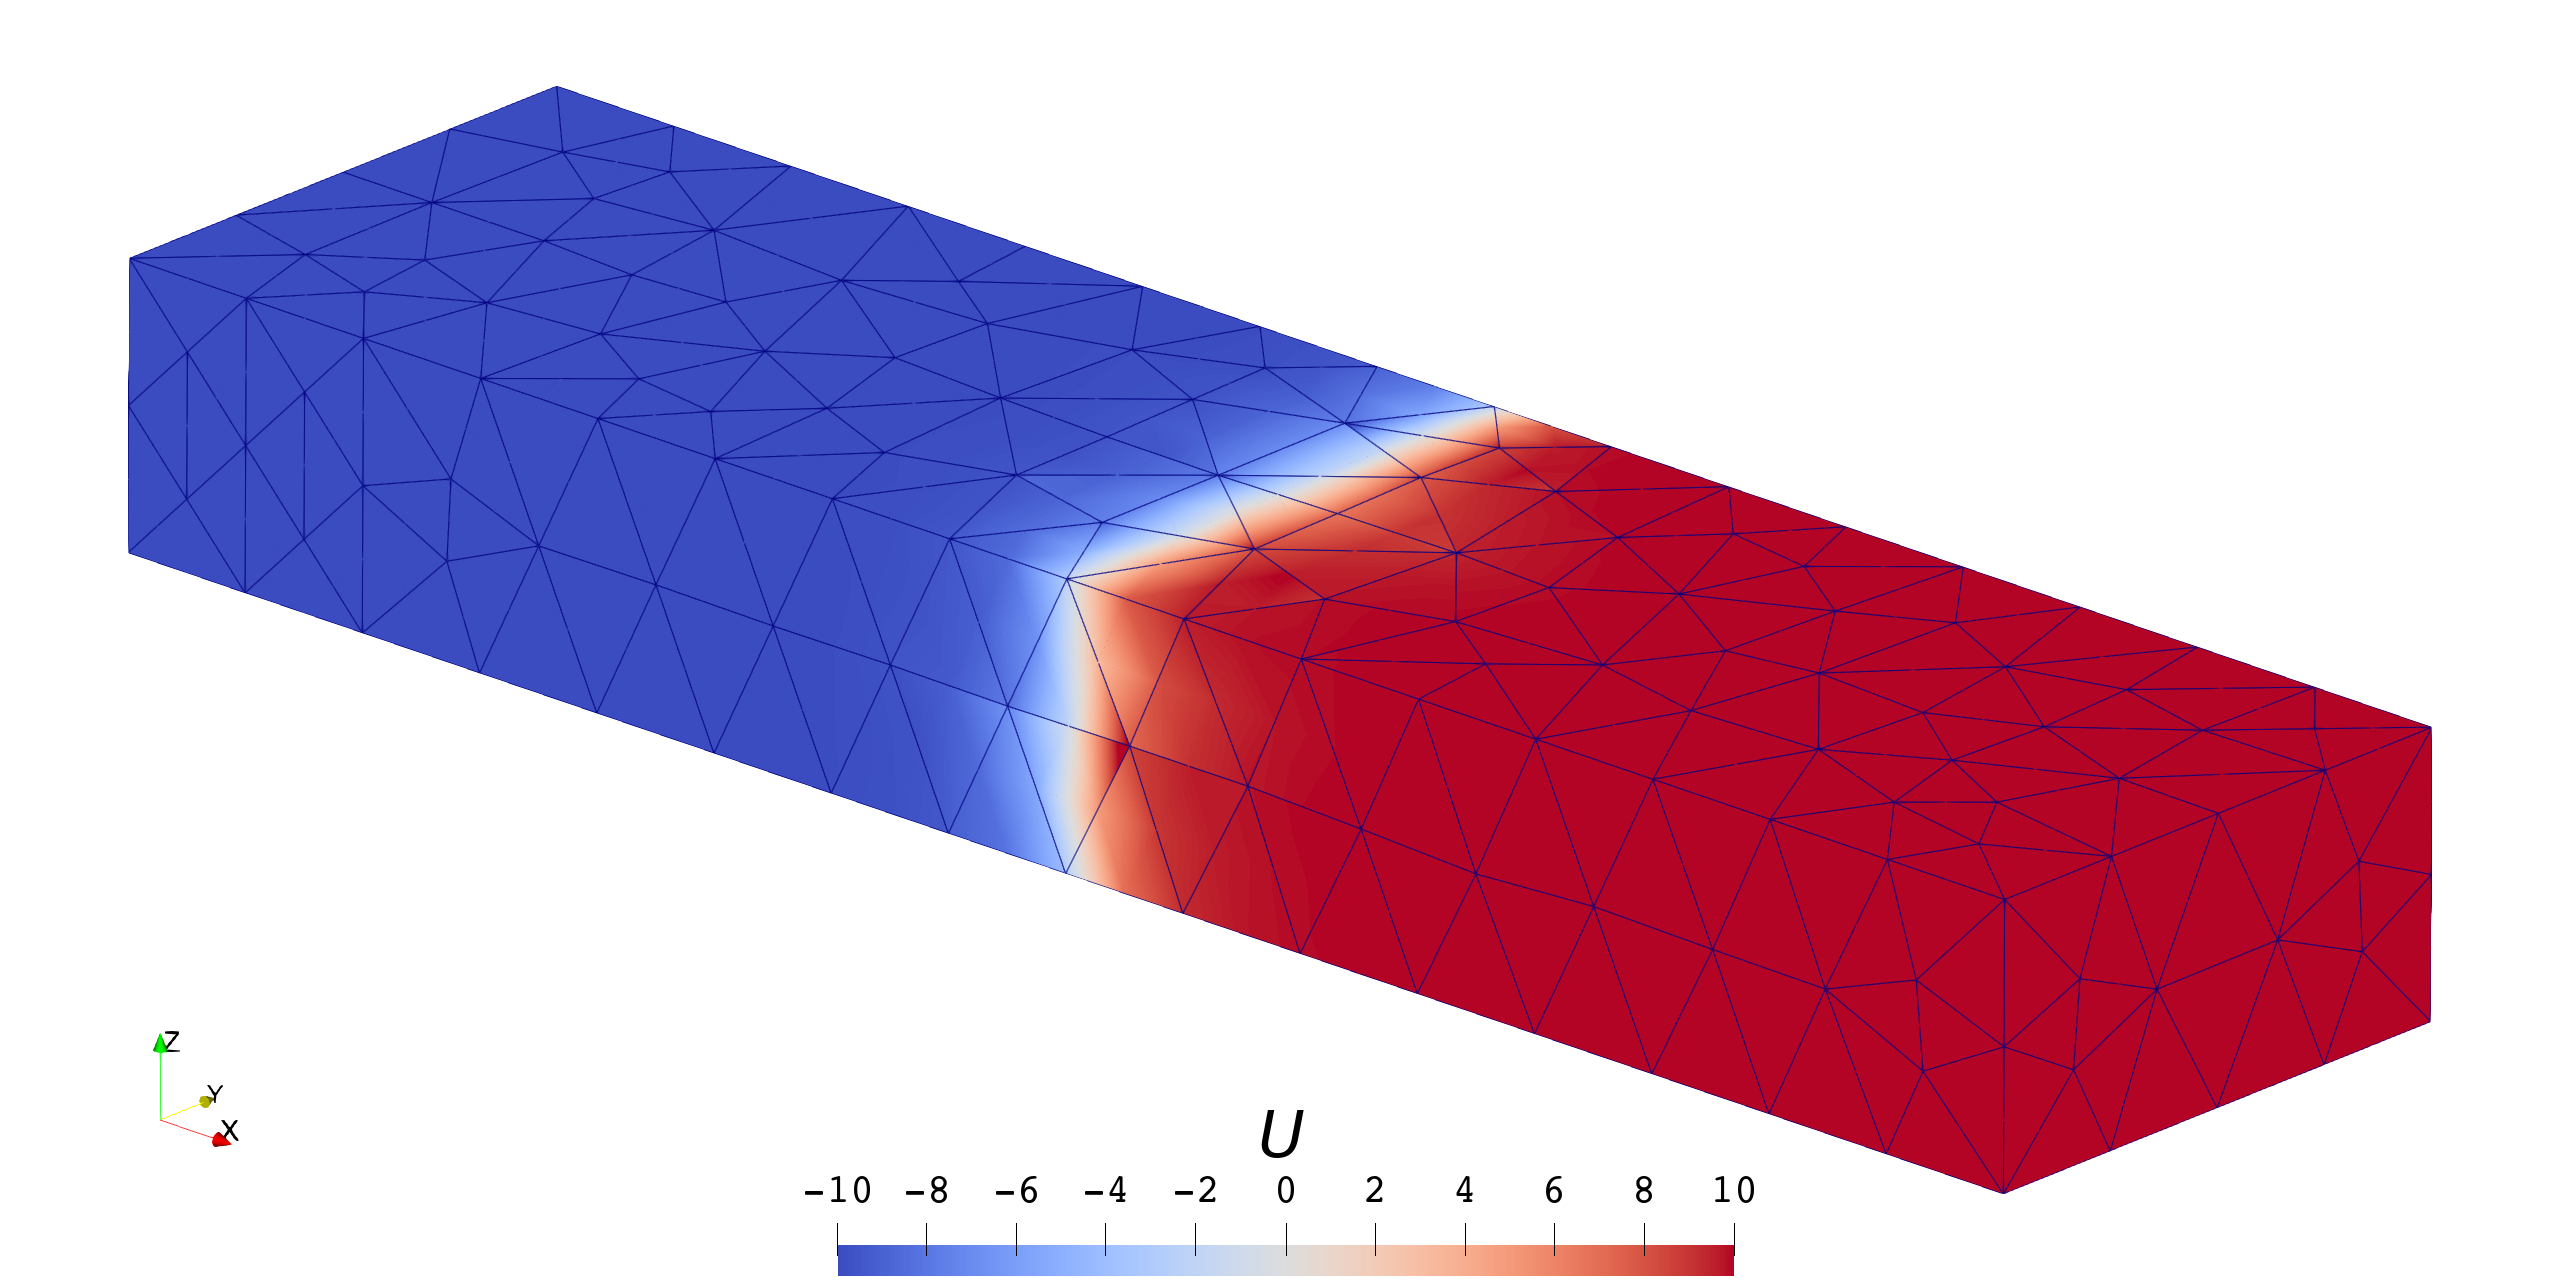
\includegraphics[width=1\textwidth,height=0.4\textheight,keepaspectratio]{../mdpi/figures/linear_scalar/p=3_h=2^-2}
\par\end{centering}
}
\par\end{centering}
\centering{}\caption{\label{fig:linear_scalar_contour}在只含四面体单元的非结构网格上所得\nameref{prob:=007EBF=006027=005355=006CE2=005E73=006D41}问题在
$t=0.2$ 时刻的 RKDG 近似解}
\end{figure}

为了进一步体现单元尺寸与求解器阶数对数值解精度的影响,图 \ref{fig:linear_scalar_h_vary}–\ref{fig:linear_scalar_p_vary}
给出了沿纵向对称轴 ($y=0.5,\,z=0.25$) 均匀分布的 1001 个采样点处的函数值。二者分别体现了加密网格(减小
$h$)与增加阶数(增大 $p$)对数值解精度的提高。

\begin{figure}[h!]
\begin{centering}
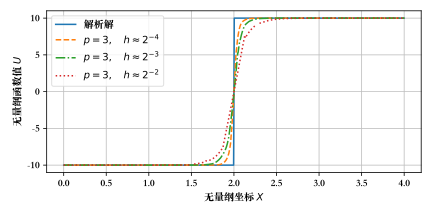
\includegraphics[width=1\textwidth,height=0.3\textheight,keepaspectratio]{figures/linear_scalar/h_vary}
\par\end{centering}
\caption{\label{fig:linear_scalar_h_vary}同一求解器在不同网格上所得\nameref{prob:=007EBF=006027=005355=006CE2=005E73=006D41}问题在
$t=0.2$ 时刻的近似解之间的比较}
\end{figure}

\begin{figure}[h!]
\begin{centering}
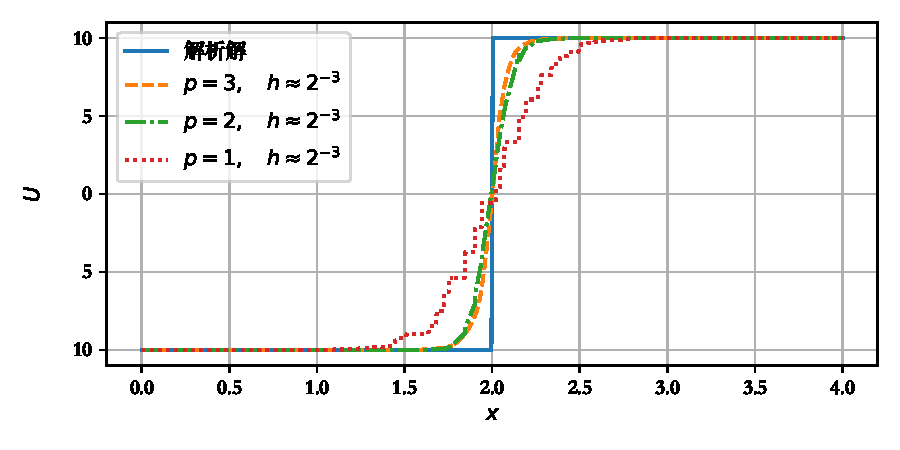
\includegraphics[width=1\textwidth,height=0.3\textheight,keepaspectratio]{figures/linear_scalar/p_vary}
\par\end{centering}
\caption{\label{fig:linear_scalar_p_vary}不同求解器在同一网格上所得\nameref{prob:=007EBF=006027=005355=006CE2=005E73=006D41}问题在
$t=0.2$ 时刻的近似解之间的比较}
\end{figure}

表 \ref{tab:linear_accuracy} 列出了各种求解器–网格 ($p$–$h$) 组合的全局误差测量值。这里的“全局误差”定义为
\begin{equation}
\varepsilon(t)=\sum_{i\in I_{V}}\int_{V_{i}}\left|U^{h}(x,y,z,t)-U^{\star}(x,y,z,t)\right|.\label{eq:global-error}
\end{equation}

表 \ref{tab:linear_accuracy} 中的数据验证了前文定性观察得出的结论,即 (1) 细 ($h\approx1/32$)
网格上的低阶 ($p=1$) 数值解,与粗 ($h\approx1/4$) 网格上的高阶 ($p=3$) 数值解精度相当;(2)
加密网格(减小 $h$)或增加阶数(增大 $p$)都能提高数值解精度。

\begin{table}
\caption{\label{tab:linear_accuracy}各种求解器–网格组合所得\nameref{prob:=007EBF=006027=005355=006CE2=005E73=006D41}问题近似解的全局误差}

\centering{}%
\begin{tabular}{ccccc}
\toprule 
\diagbox{$p$}{$\eval{\varepsilon}_{t=0.2}$}{$h$} & $2^{-2}$ & $2^{-3}$ & $2^{-4}$ & $2^{-5}$\tabularnewline
\midrule
1 & 2.858 & 2.095 & 1.524 & 1.108\tabularnewline
2 & 1.258 & 0.771 & 0.463 & 0.275\tabularnewline
3 & 1.021 & 0.590 & 0.341 & \tabularnewline
\bottomrule
\end{tabular}
\end{table}

表 \ref{tab:linear_cost} 列出了各种求解器–网格 ($p$–$h$) 组合的运行时间。这里的“运行时间”含数据结构初始化及文件读写等操作,均为在主频为
2.7 GHz 的单核处理器上测得。需要承认的是,表 \ref{tab:linear_cost} 中的数据夸大了低阶 RKDG 求解器的运行时间,这是因为就间断伽辽金有限元法而言,低阶
RKDG 求解器本可以采用与之相对应的低阶数值积分器。但为了公平地计算式 (\ref{eq:global-error}) 所定义的全局误差,本节所展示的各阶
RKDG 求解器使用了同一个高阶数值积分器,即在四面体单元上具有 6 阶代数精度的 24 点积分器。即便如此,由表 \ref{tab:linear_cost}
所列数据依然可知:在数值解精度大致相当的情况下,高阶 ($p=3$) 求解器在粗 ($h\approx1/4$) 网格上所消耗的运行时间
(4.147 s) 远小于低阶 ($p=1$) 求解器在细 ($h\approx1/32$) 网格上的所消耗的运行时间(306.293
s 或按 $1/24$ 换算后的 12.762 s)。

\begin{table}
\caption{\label{tab:linear_cost}各种求解器–网格组合所得\nameref{prob:=007EBF=006027=005355=006CE2=005E73=006D41}问题的运行时间}

\centering{}%
\begin{tabular}{ccccc}
\toprule 
\diagbox{$p$}{$T$ (s)}{$h$} & $2^{-2}$ & $2^{-3}$ & $2^{-4}$ & $2^{-5}$\tabularnewline
\midrule
1 & 0.373 & 1.129 & 16.533 & 306.293\tabularnewline
2 & 1.580 & 14.894 & 253.821 & 4986.391\tabularnewline
3 & 4.147 & 61.425 & 906.914 & \tabularnewline
\bottomrule
\end{tabular}
\end{table}

以上结果表明:高阶 RKDG 求解器具有较高的“性价比”。这里的“性”指全局精度,“价”指运行时间。

\subsection{线性双波平流问题}
\begin{problem}
[线性双波平流]\label{prob:=007EBF=006027=0053CC=006CE2=005E73=006D41}在方程
(\ref{eq:linear_system}) 中,令
\begin{equation}
\underline{U}(\vec{x},t)=\begin{bmatrix}U_{1}(x,y,z,t)\\
U_{2}(x,y,z,t)
\end{bmatrix},\qquad\underline{A}^{x}=\begin{bmatrix}6 & -2\\
-2 & 6
\end{bmatrix},\qquad\underline{A}^{y}=\underline{A}^{z}=\begin{bmatrix}0 & 0\\
0 & 0
\end{bmatrix},
\end{equation}
由此得线性双波方程组
\begin{equation}
\begin{cases}
\partial_{t}U_{1}+6\partial_{x}U_{1}-2\partial_{x}U_{2}=0,\\
\partial_{t}U_{2}-2\partial_{x}U_{1}+6\partial_{x}U_{2}=0.
\end{cases}\label{eq:linear_double_wave}
\end{equation}
求满足此方程组与边界条件
\begin{equation}
\underline{U}(x=0,y,z,t)=\begin{bmatrix}0\\
0
\end{bmatrix}\eqqcolon\underline{U}_{\mathrm{L}},\qquad\underline{U}(x=4,y,z,t)=\begin{bmatrix}12\\
-4
\end{bmatrix}\eqqcolon\underline{U}_{\mathrm{R}},
\end{equation}
及初始条件
\begin{equation}
\underline{U}(x,y,z,t=0)=\underline{U}_{\mathrm{R}}
\end{equation}
的广义解。
\end{problem}

为获得其解析解,先对 $\underline{A}^{x}$ 作特征分解,得到
\begin{equation}
\underbrace{\begin{bmatrix}6 & -2\\
-2 & 6
\end{bmatrix}}_{\underline{A}^{x}}=\underbrace{\begin{bmatrix}1 & 1\\
-1 & 1
\end{bmatrix}}_{\underline{R}^{x}}\underbrace{\begin{bmatrix}8\\
 & 4
\end{bmatrix}}_{\underline{\varLambda}^{x}}\underbrace{\begin{bmatrix}1/2 & -1/2\\
1/2 & 1/2
\end{bmatrix}}_{\underline{L}^{x}}.
\end{equation}
通过引入特征变量 $\underline{V}\coloneqq\underline{L}^{x}\,\underline{U}$,即
\begin{equation}
\begin{bmatrix}V_{1}\\
V_{2}
\end{bmatrix}\coloneqq\begin{bmatrix}1/2 & -1/2\\
1/2 & 1/2
\end{bmatrix}\begin{bmatrix}U_{1}\\
U_{2}
\end{bmatrix}=\frac{1}{2}\begin{bmatrix}U_{1}-U_{2}\\
U_{1}+U_{2}
\end{bmatrix},
\end{equation}
可以将边界条件转化为
\begin{equation}
\underline{V}_{\mathrm{L}}=\underline{L}^{x}\,\underline{U}_{\mathrm{L}}=\begin{bmatrix}0\\
0
\end{bmatrix},\qquad\underline{V}_{\mathrm{R}}=\underline{L}^{x}\,\underline{U}_{\mathrm{R}}=\begin{bmatrix}8\\
4
\end{bmatrix},
\end{equation}
并将方程组 (\ref{eq:linear_double_wave}) 解耦为
\begin{equation}
\begin{cases}
\left(\partial_{t}+8\partial_{x}\right)V_{1}=0,\\
\left(\partial_{t}+4\partial_{x}\right)V_{2}=0.
\end{cases}
\end{equation}
由此得到两个独立的初边值问题,它们的解析解分别为
\begin{equation}
V_{1}^{\star}(x,y,z,t)=\begin{cases}
0, & x<8t,\\
8, & x>8t,
\end{cases}\qquad V_{2}^{\star}(x,y,z,t)=\begin{cases}
0, & x<4t,\\
4, & x>4t.
\end{cases}
\end{equation}
在此基础上,原问题 \ref{prob:=007EBF=006027=0053CC=006CE2=005E73=006D41} 的解可通过特征变量到守恒变量的反变换
$\underline{U}^{\star}=\underline{R}^{x}\,\underline{V}^{\star}$
得到:
\begin{equation}
\underline{U}^{\star}(\vec{x},t)=\begin{bmatrix}V_{2}^{\star}+V_{1}^{\star}\\
V_{2}^{\star}-V_{1}^{\star}
\end{bmatrix}=\begin{cases}
\underline{U}_{\mathrm{L}}, & x/t<4,\\
\underline{U}_{\mathrm{M}}, & x/t\in(4,8),\\
\underline{U}_{\mathrm{R}}, & x/t>8,
\end{cases}\label{eq:linear_double_wave_solution}
\end{equation}
其中
\begin{equation}
\underline{U}_{\mathrm{L}}=\begin{bmatrix}0\\
0
\end{bmatrix},\qquad\underline{U}_{\mathrm{M}}=\begin{bmatrix}4\\
4
\end{bmatrix},\qquad\underline{U}_{\mathrm{R}}=\begin{bmatrix}12\\
-4
\end{bmatrix}.
\end{equation}

此解析解可以被用来定量地评估数值求解器的性能。本小节使用图 \ref{subfig:linear_scalar_p=00003D3_h=00003D2^-3}
所示的网格,测试了四种求解器–限制器组合,所得结果如图 \ref{fig:linear_double_wave_u1}–\ref{fig:linear_double_wave_sample_u2}
所示,其中图 \ref{fig:linear_double_wave_sample_u1}–\ref{fig:linear_double_wave_sample_u2}
依然为沿纵向对称轴均匀分布的 1001 个采样点处的函数值。

\begin{figure}[h!]
\begin{centering}
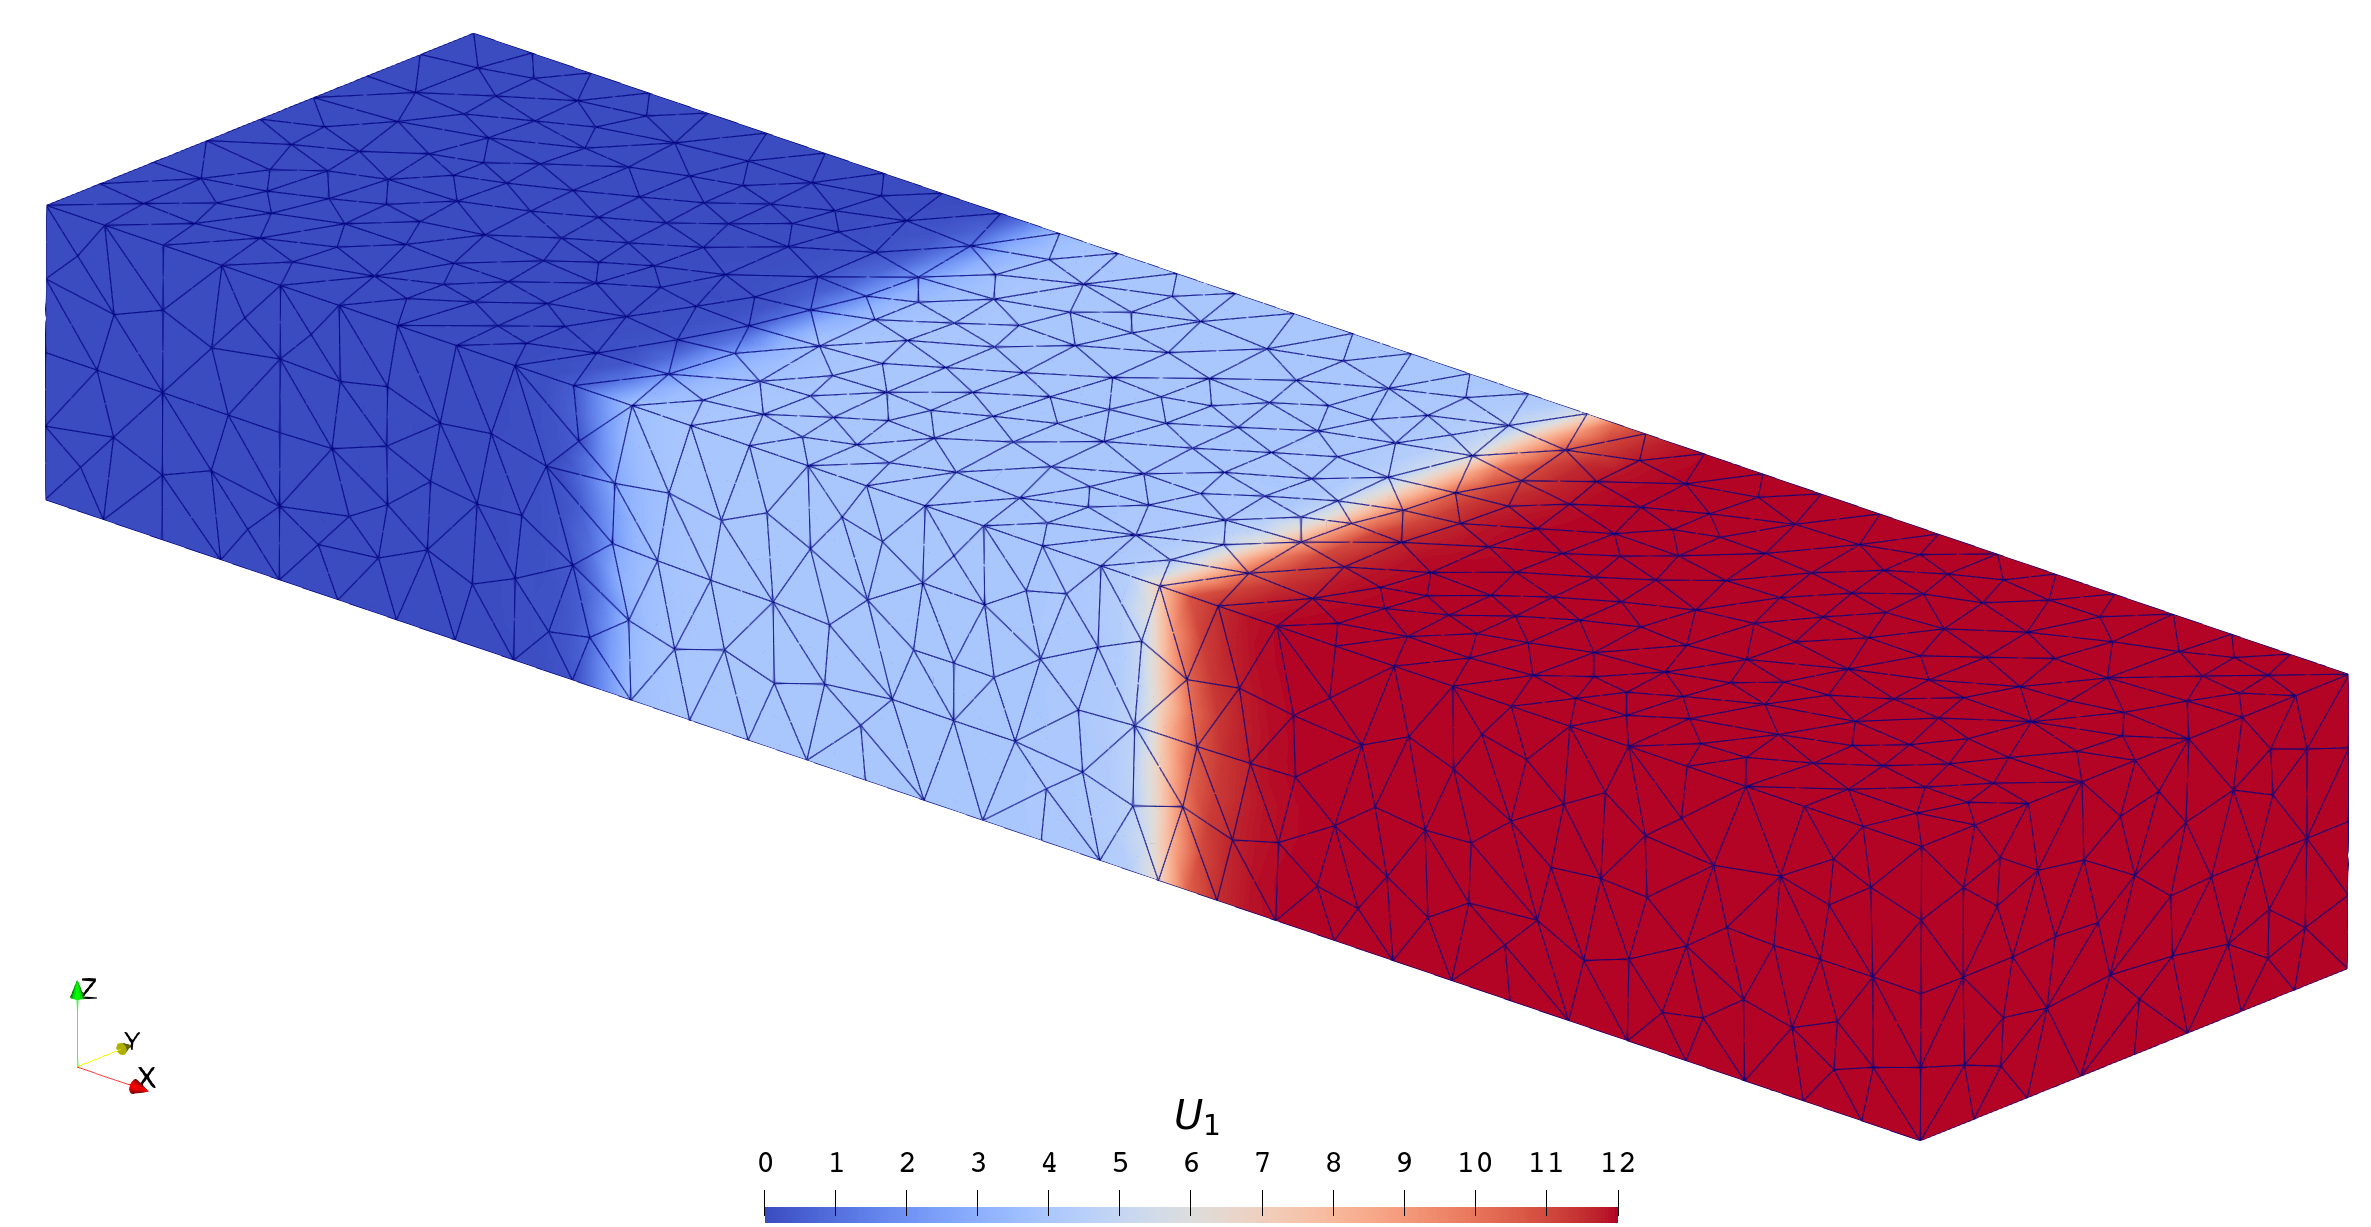
\includegraphics[width=1\textwidth]{../mdpi/figures/linear_system/u_1_contour}
\par\end{centering}
\caption{\label{fig:linear_double_wave_u1}\nameref{prob:=007EBF=006027=0053CC=006CE2=005E73=006D41}问题
$U_{1}(x,y,z,t=0.3)$ 的 RK3/DG3 近似解}
\end{figure}

\begin{figure}[h!]
\begin{centering}
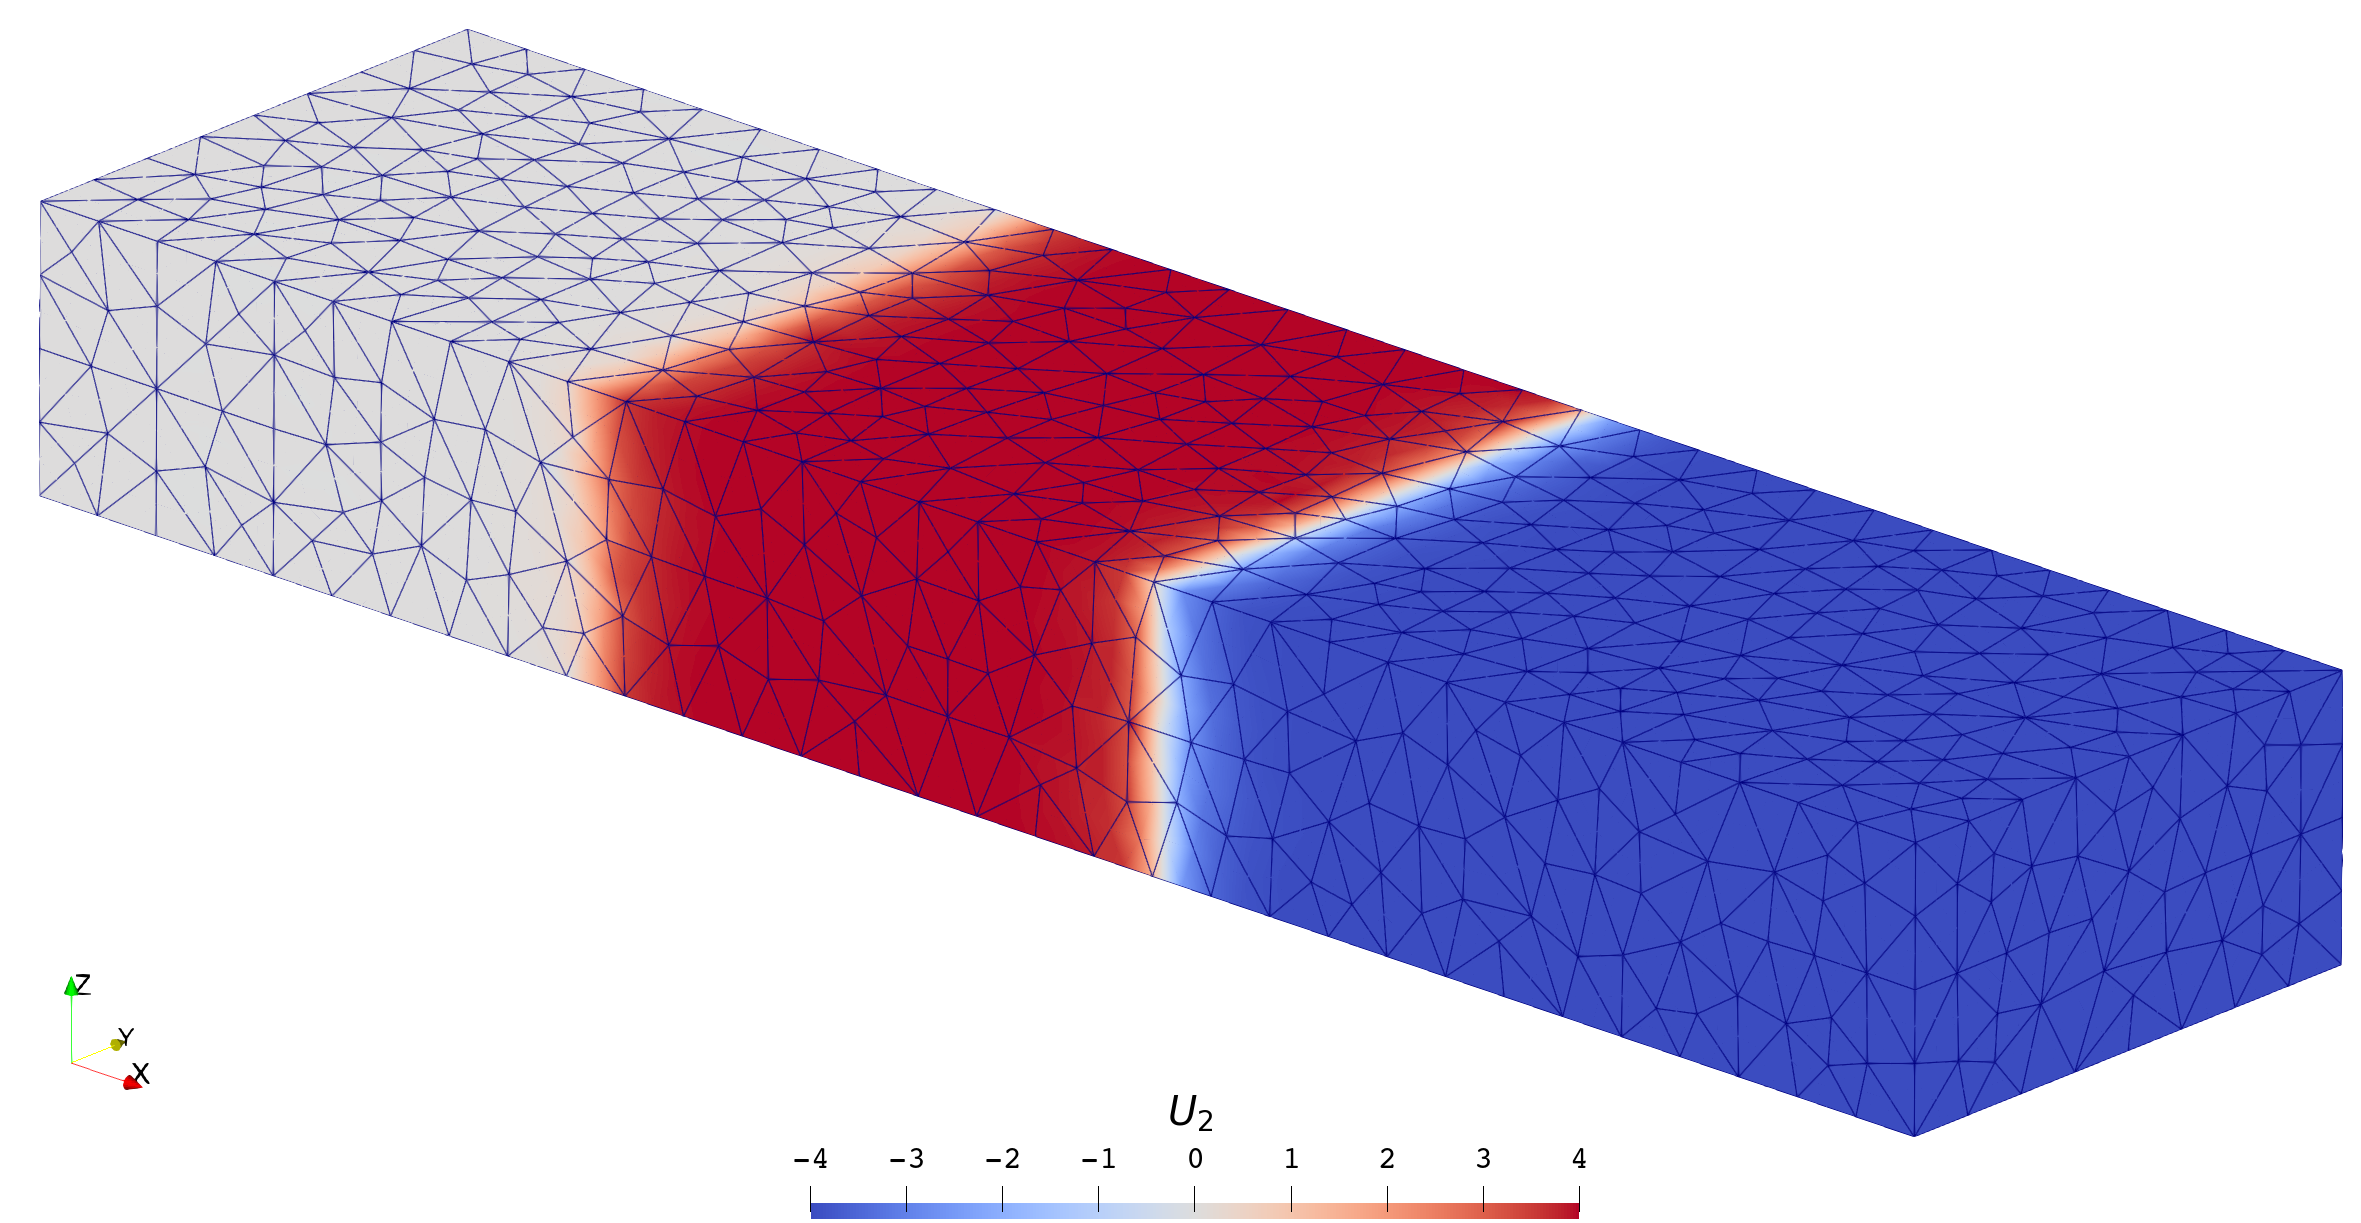
\includegraphics[width=1\textwidth]{../mdpi/figures/linear_system/u_2_contour}
\par\end{centering}
\caption{\label{fig:linear_double_wave_u2}\nameref{prob:=007EBF=006027=0053CC=006CE2=005E73=006D41}问题
$U_{2}(x,y,z,t=0.3)$ 的 RK3/DG3 近似解}
\end{figure}

\begin{figure}[h!]
\begin{centering}
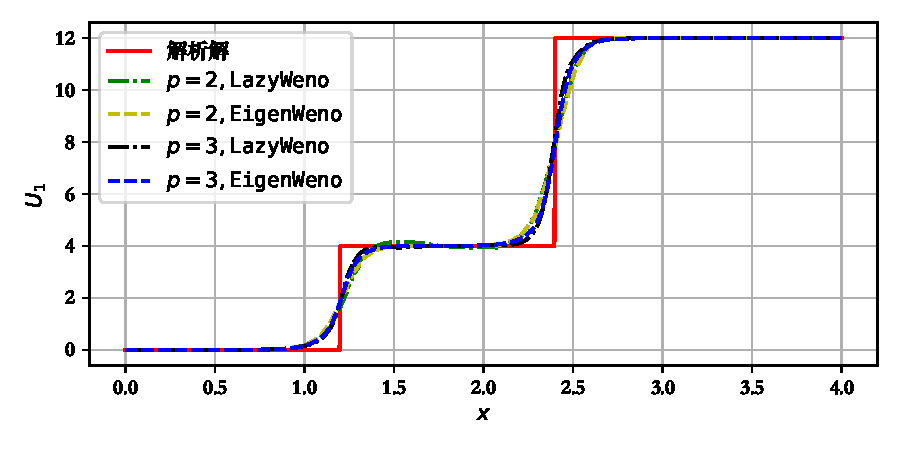
\includegraphics[width=1\textwidth,height=0.3\textheight]{figures/linear_system/u_1}
\par\end{centering}
\caption{\label{fig:linear_double_wave_sample_u1}不同求解器–限制器组合在同一网格上所得\nameref{prob:=007EBF=006027=0053CC=006CE2=005E73=006D41}问题
$U_{1}(x,y=0.5,z=0.25,t=0.3)$ 近似解之间的比较}
\end{figure}

\begin{figure}[h!]
\begin{centering}
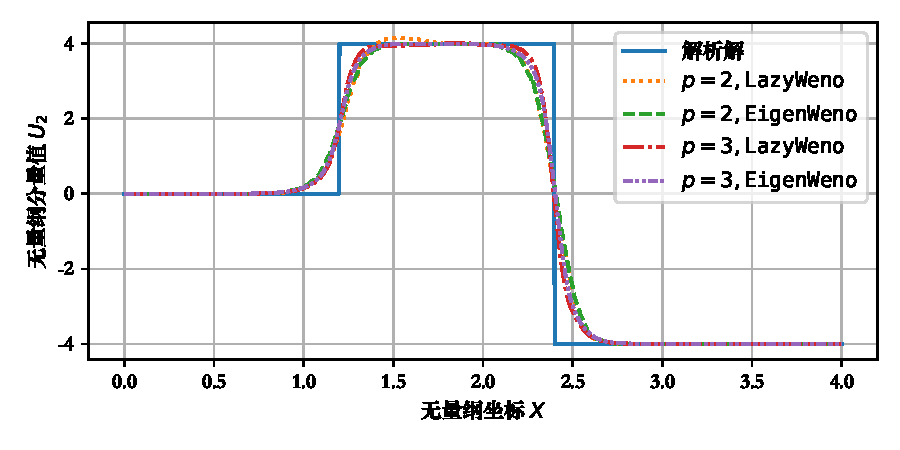
\includegraphics[width=1\textwidth,height=0.3\textheight]{figures/linear_system/u_2}
\par\end{centering}
\caption{\label{fig:linear_double_wave_sample_u2}不同求解器–限制器组合在同一网格上所得\nameref{prob:=007EBF=006027=0053CC=006CE2=005E73=006D41}问题
$U_{2}(x,y=0.5,z=0.25,t=0.3)$ 近似解之间的比较}
\end{figure}

为了更清晰地展示各种求解器–限制器组合的效果,图 \ref{fig:linear_double_wave_error} 比较了以上四种数值解的绝对误差。这里的“绝对误差”定义为
\begin{equation}
\varepsilon(x)=\left(\left|U_{1}^{h}-U_{1}^{\star}\right|+\left|U_{2}^{h}-U_{2}^{\star}\right|\right)_{y=0.5,\,z=0.25,\,t=0.3}.
\end{equation}

\begin{figure}[h!]
\begin{centering}
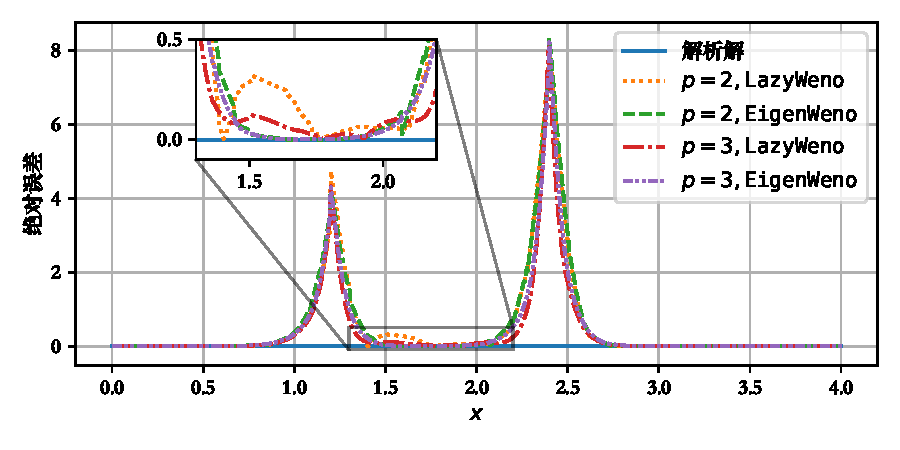
\includegraphics[width=1\textwidth,height=0.3\textheight]{figures/linear_system/error}
\par\end{centering}
\caption{\label{fig:linear_double_wave_error}\nameref{prob:=007EBF=006027=0053CC=006CE2=005E73=006D41}问题近似解(图
\ref{fig:linear_double_wave_sample_u1}–\ref{fig:linear_double_wave_sample_u2})的绝对误差之比较}
\end{figure}

由以上结果可知:\texttt{LazyWeno} 及 \texttt{EigenWeno} 这两种限制器都能有效地压制非物理振荡,且后者压制振荡的效果优于前者。基于此结论,本文剩余部分的所有算例都将全部采用
\texttt{EigenWeno} 限制器,并且所有算例均为描述无黏可压缩流动的三维欧拉方程
\begin{equation}
\partial_{t}\begin{bmatrix}\rho\\
\rho u_{x}\\
\rho u_{y}\\
\rho u_{z}\\
\rho e_{0}
\end{bmatrix}+\partial_{x}\begin{bmatrix}\rho u_{x}\\
\rho u_{x}u_{x}+p\\
\rho u_{y}u_{x}\\
\rho u_{z}u_{x}\\
\rho h_{0}u_{x}
\end{bmatrix}+\partial_{y}\begin{bmatrix}\rho u_{y}\\
\rho u_{x}u_{y}\\
\rho u_{y}u_{y}+p\\
\rho u_{z}u_{y}\\
\rho h_{0}u_{y}
\end{bmatrix}+\partial_{z}\begin{bmatrix}\rho u_{z}\\
\rho u_{x}u_{z}\\
\rho u_{y}u_{z}\\
\rho u_{z}u_{z}+p\\
\rho h_{0}u_{z}
\end{bmatrix}=\begin{bmatrix}0\\
0\\
0\\
0\\
0
\end{bmatrix}\label{eq:euler_system}
\end{equation}
与某些初始条件及边界条件所构成的初边值问题。

\section{基于一维流场数值精确解的定量验证}

激波管问题是欧拉方程的黎曼问题。其精确解含有激波、膨胀波、接触间断中的一种或多种,有时还会形成真空;又因其流场边界几何外形简单,初始条件、边界条件非常容易设置,自其被提出以来便被用作考核欧拉方程数值解的标准算例。

它们通常被简化为一维问题,但本文将其用于验证三维欧拉方程求解器的正确性,因此需要在三维空间内重新给出其定义。本小节的所有问题都在三维区间
$[0.0,5.0]\times[0.0,1.0]\times[0.0,0.5]$ 内求解,且平行于 $x$ 轴的边界均设为固体壁面。尽管这些问题没有封闭形式的解析解,但基于文献 \cite{Toro_2009}
介绍的方法,辅之以精度充分高的非线性代数方程求解器,仍然可以得到精度任意高的近似解。这种近似解的精度可以充分高,以至于其与实数范围内的精确解具有相同的(有限位)浮点数表示。若无特别说明,本文剩余部分提到的“精确解”都是指“浮点数范围内的精确解”或“计算机上的精确解”。

\subsection{Sod 激波管问题}
\begin{problem}
[Sod 激波管]\label{prob:Sod-=006FC0=006CE2=007BA1}在时间范围 $t\in[0.0,1.0]$
内,求满足三维欧拉方程 (\ref{eq:euler_system}) 及边界条件
\begin{equation}
\begin{bmatrix}\rho & u_{x} & u_{y} & u_{z} & p\end{bmatrix}=\begin{cases}
\begin{bmatrix}1 & 0 & 0 & 0 & 1\end{bmatrix}, & x=0,\\
\begin{bmatrix}\frac{1}{8} & 0 & 0 & 0 & \frac{1}{10}\end{bmatrix}, & x=5,
\end{cases}
\end{equation}
与初始条件

\begin{equation}
\begin{bmatrix}\rho & u_{x} & u_{y} & u_{z} & p\end{bmatrix}_{t=0}=\begin{cases}
\begin{bmatrix}\rho & u_{x} & u_{y} & u_{z} & p\end{bmatrix}_{x=0}, & x<2.5,\\
\begin{bmatrix}\rho & u_{x} & u_{y} & u_{z} & p\end{bmatrix}_{x=5}, & x>2.5,
\end{cases}
\end{equation}
的广义解。
\end{problem}

图 \ref{fig:sod_hexa} 给出了在只含 $h\approx0.1$ 的六面体单元的非结构网格上所得该问题的 RK3/DG3
近似解。由此图中的四个间断(两个导数值间断、两个函数值间断)处的光滑过渡可知:高阶格式在间断附近引起的数值振荡得到了有效压制。这种光滑过渡在图
\ref{fig:sod_hexa_p_vary} 中更为明显。此图沿纵向对称轴 ($y=0.5,\,z=0.25$) 均匀选取了
1001 个采样点,依次画出了 RK1/DG1、RK2/DG2、RK3/DG3 近似解在这些采样点处的密度值。由图 \ref{fig:sod_hexa_p_vary}
还可知:在相同的网格上,求解器的阶数越高,数值解的精度也越高。

\begin{figure}[h!]
\begin{centering}
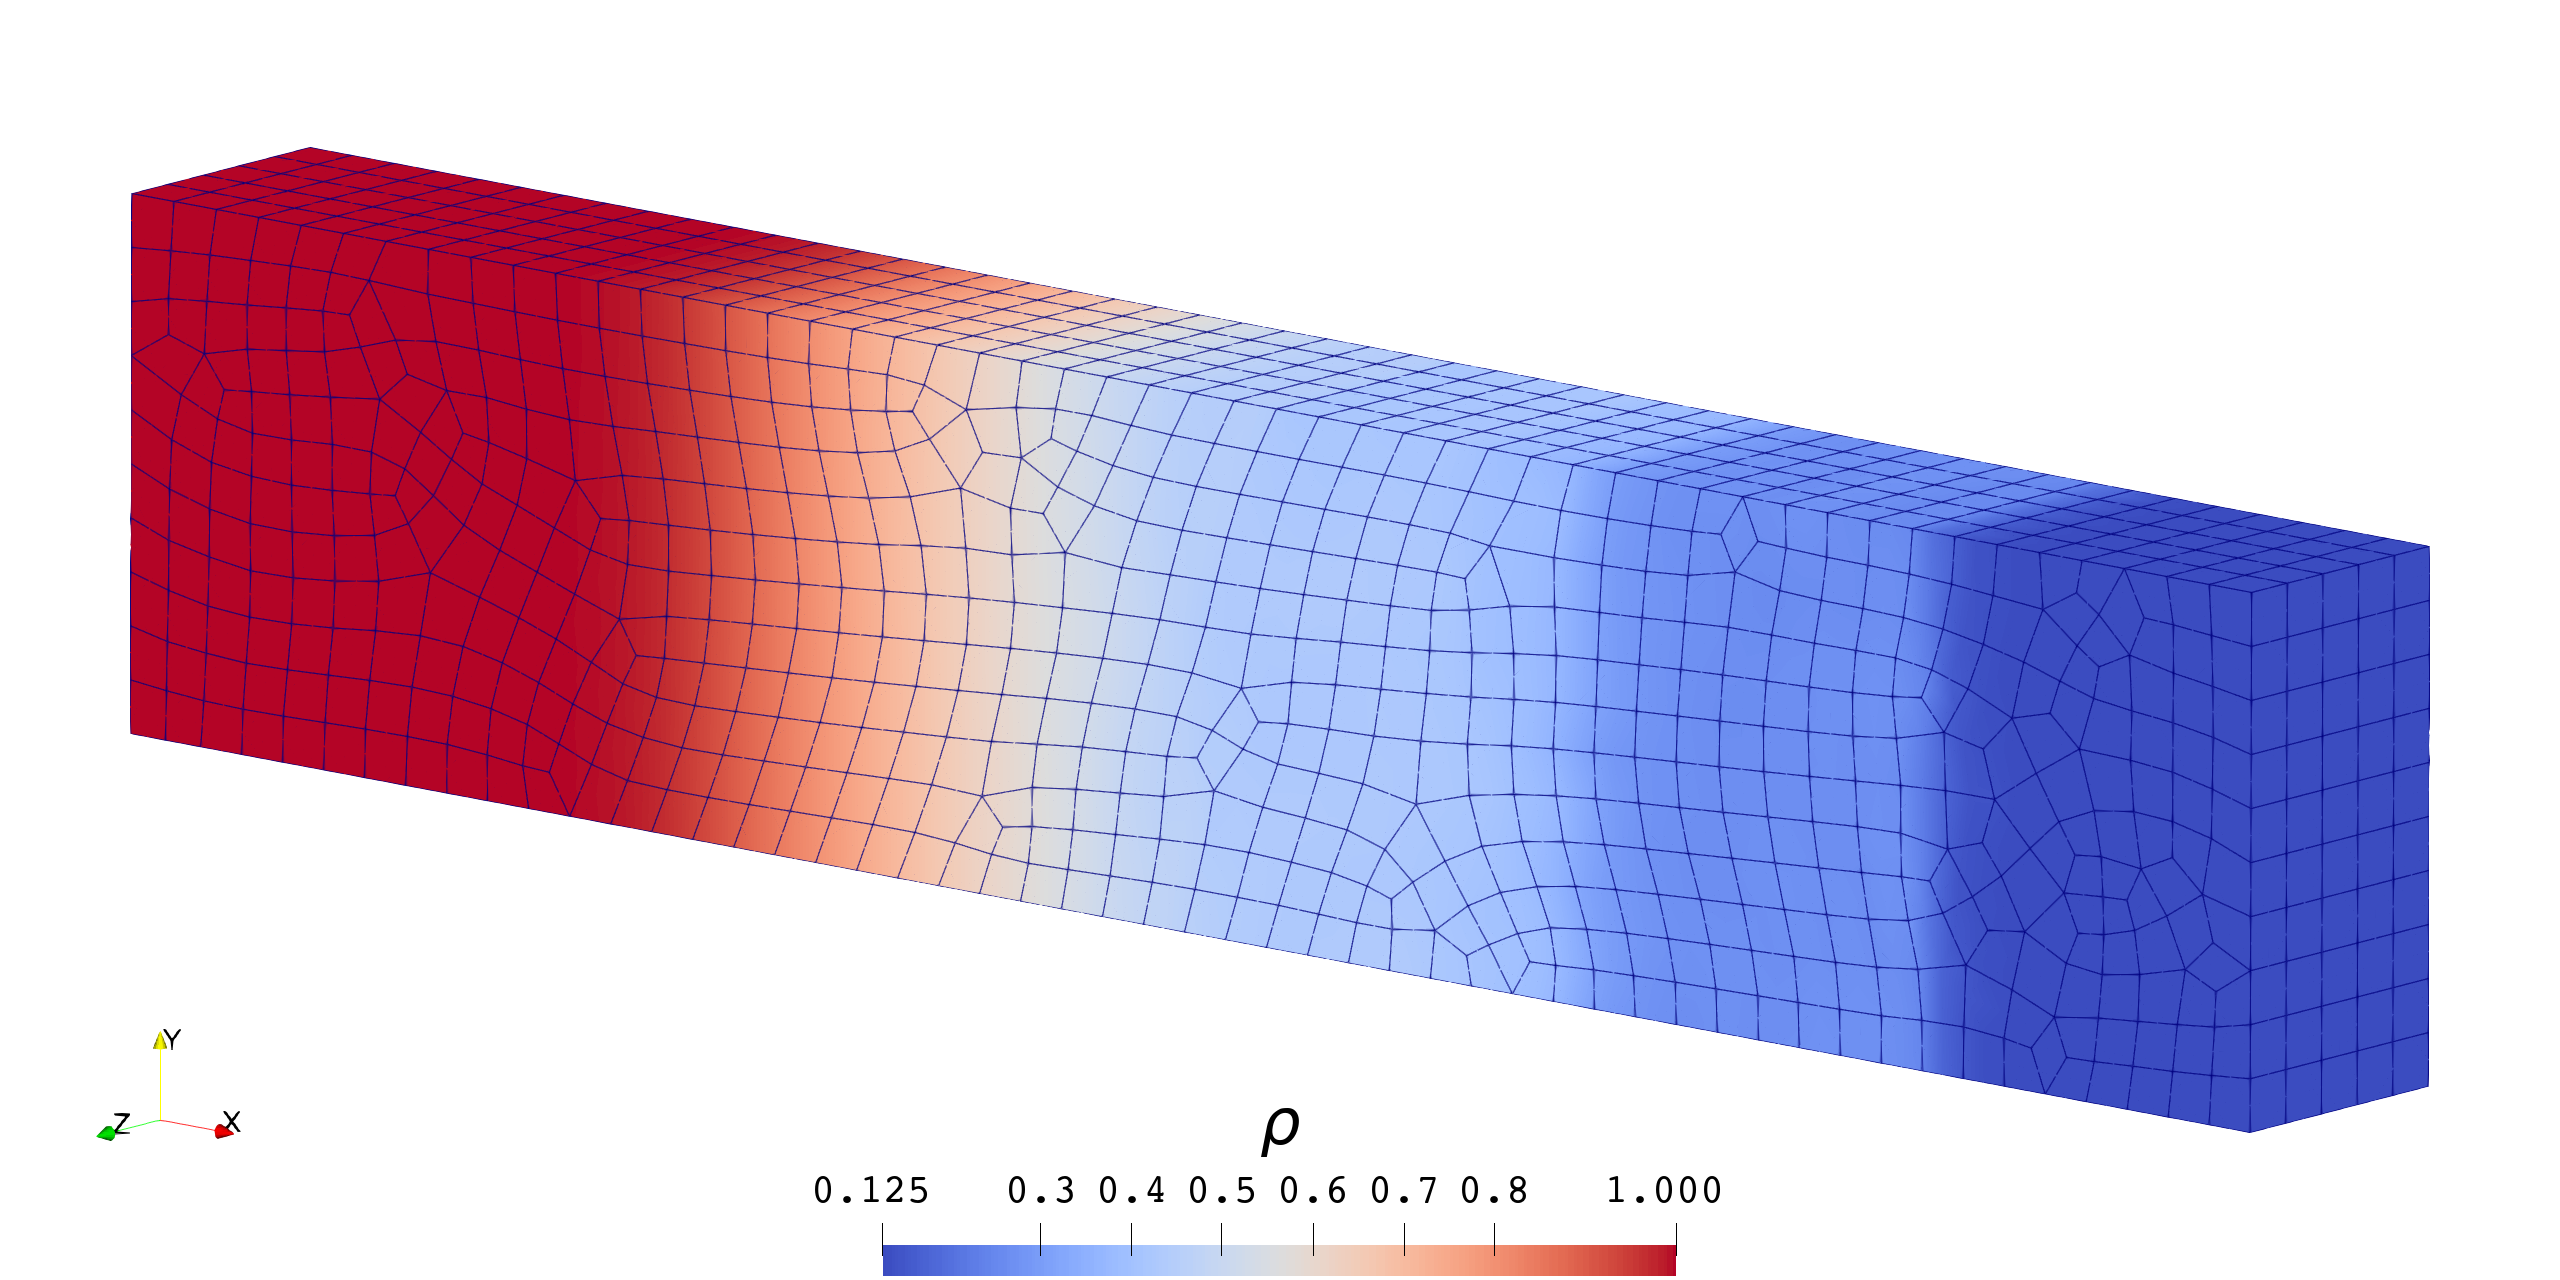
\includegraphics[width=1\textwidth]{../mdpi/figures/shock_tubes/sod/contour}
\par\end{centering}
\caption{\label{fig:sod_hexa}在只含 $h\approx0.1$ 的六面体单元的非结构网格上所得 \nameref{prob:Sod-=006FC0=006CE2=007BA1}问题
$\rho(x,y,z,t=1.0)$ 的 RK3/DG3 近似解}
\end{figure}

\begin{figure}[h!]
\begin{centering}
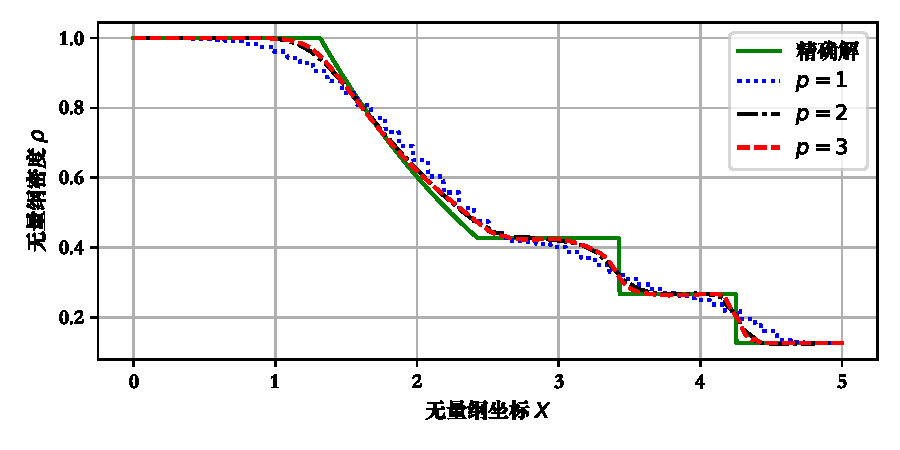
\includegraphics[width=1\textwidth,height=0.3\textheight]{figures/shock_tubes/sod/result}
\par\end{centering}
\caption{\label{fig:sod_hexa_p_vary}在只含 $h\approx0.1$ 的六面体单元的非结构网格上所得 \nameref{prob:Sod-=006FC0=006CE2=007BA1}问题
$\rho(x,y=0.5,z=0.25,t=1.0)$ 的各阶 RKDG 近似解之间的比较}
\end{figure}

为了验证上述结论的网格无关性,我们在只含 $h\approx0.1$ 的四面体单元的非结构网格上再次求解了 \nameref{prob:Sod-=006FC0=006CE2=007BA1}问题,所得结果如图
\ref{fig:sod_tetra}–\ref{fig:sod_tetra_p_vary} 所示。将它们与图 \ref{fig:sod_hexa}–\ref{fig:sod_hexa_p_vary}
比较,不难发现:无论采用何种单元,只要网格足够精细,\nameref{prob:Sod-=006FC0=006CE2=007BA1}问题的各阶
RKDG 近似解均能收敛到精确解。

\begin{figure}[h!]
\begin{centering}
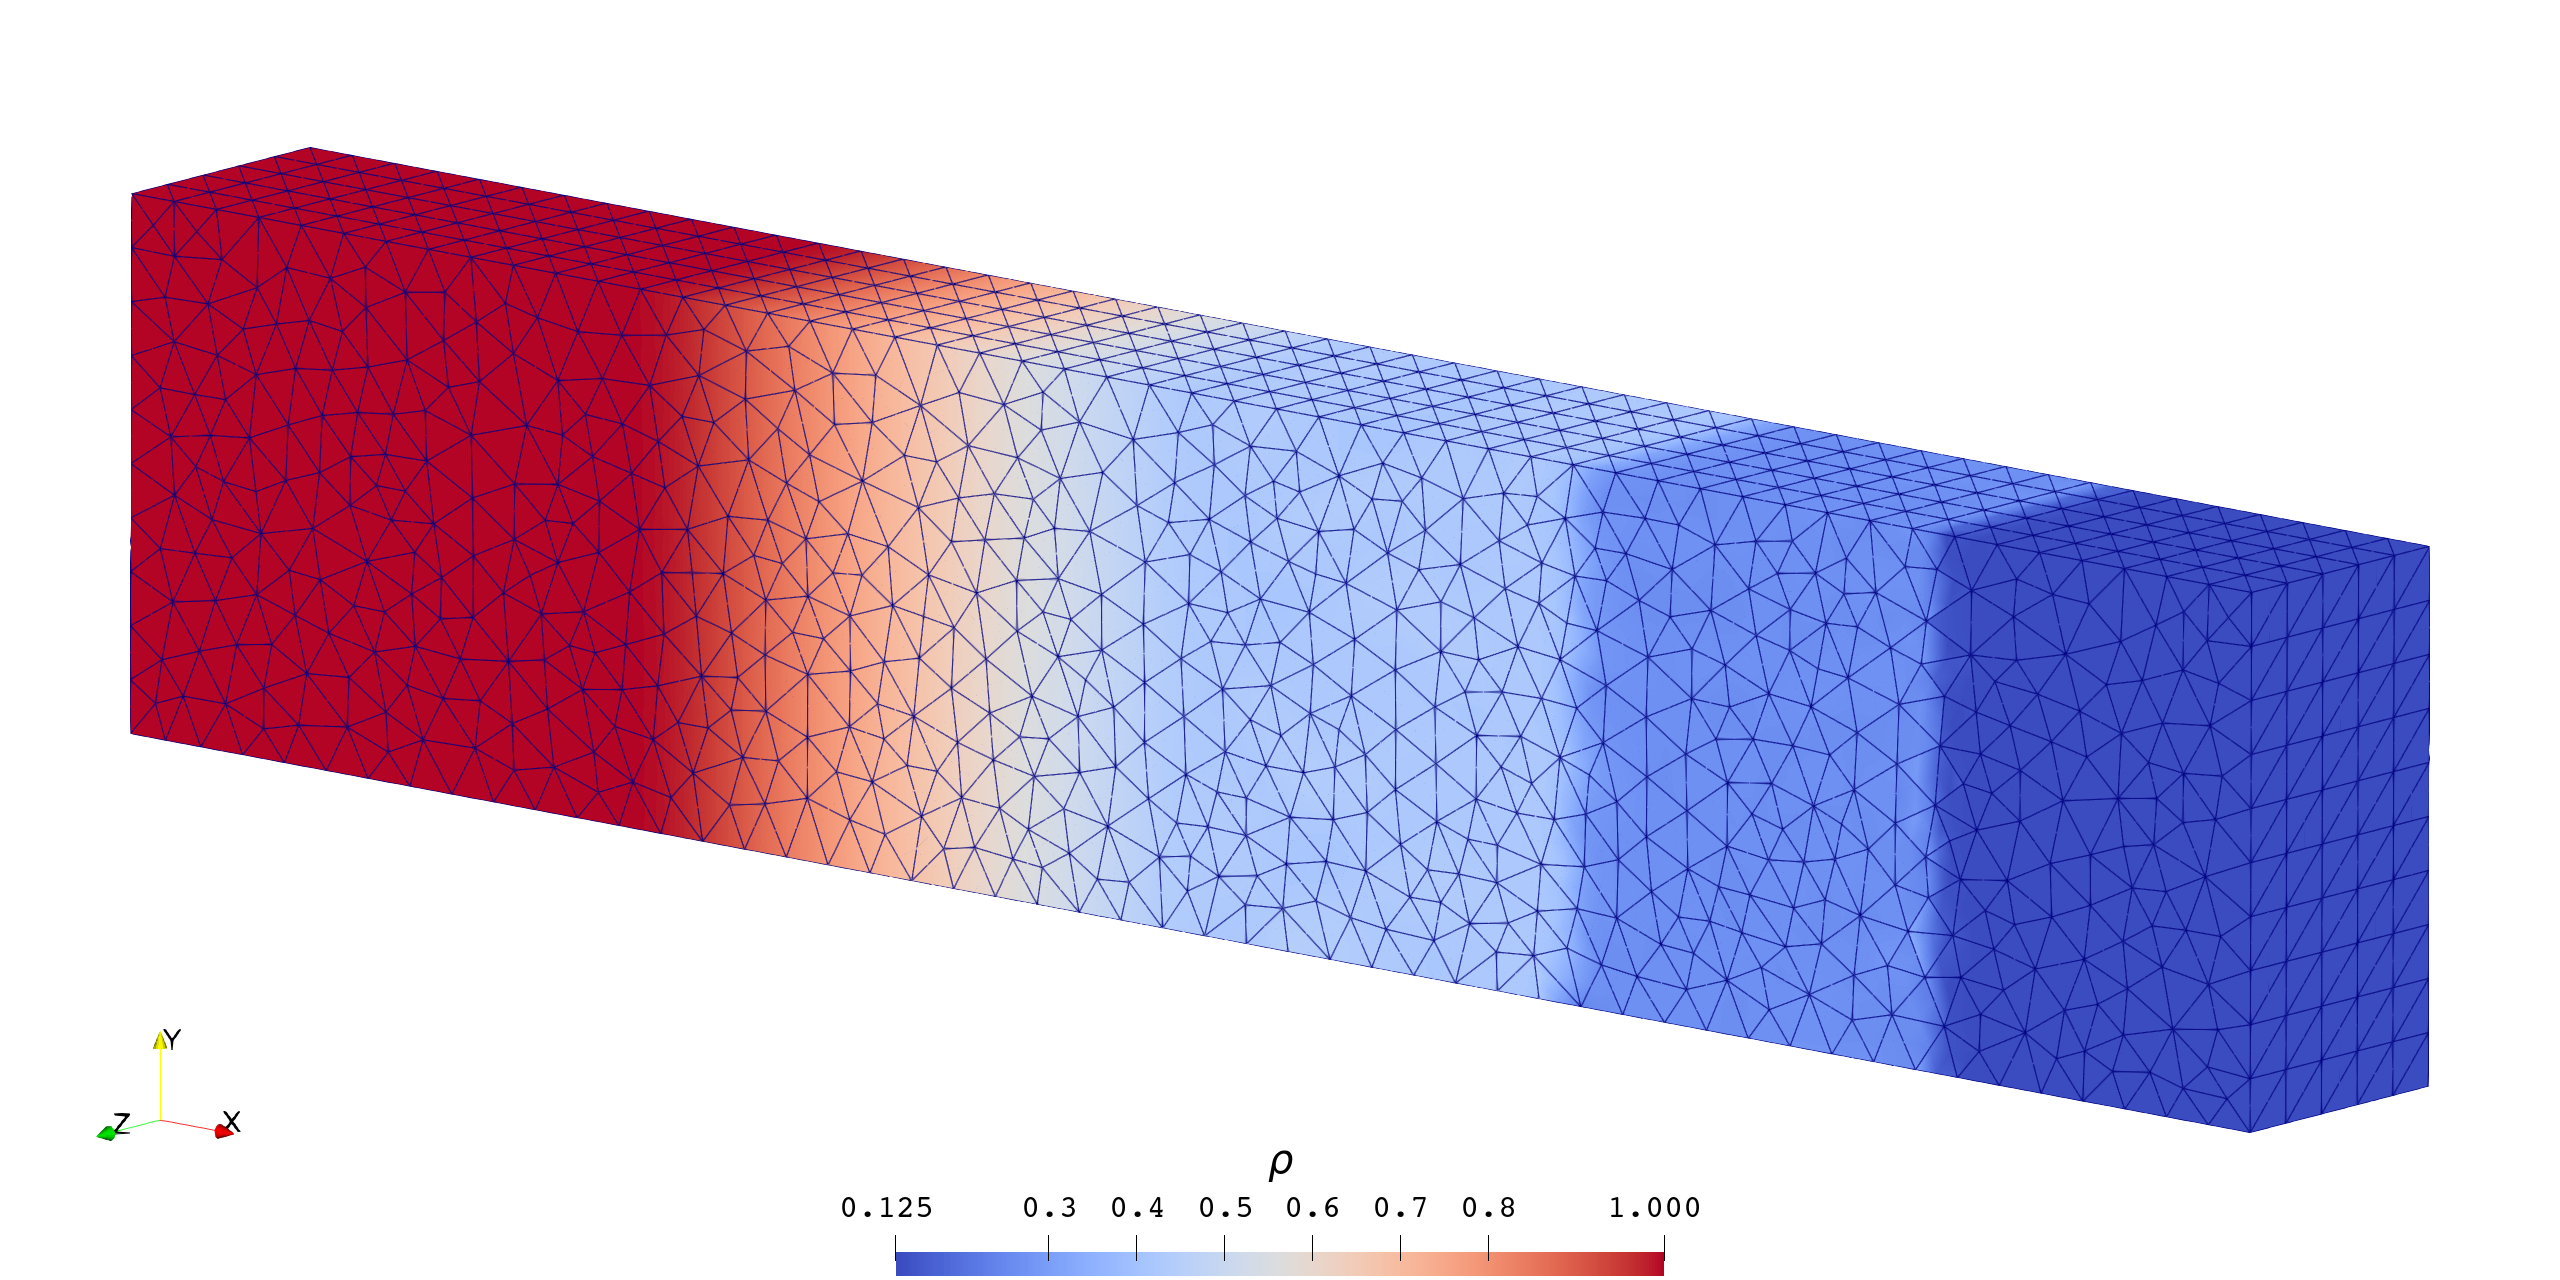
\includegraphics[width=1\textwidth]{../mdpi/figures/shock_tubes/sod/contour_tetra}
\par\end{centering}
\caption{\label{fig:sod_tetra}在只含 $h\approx0.1$ 的四面体单元的非结构网格上所得 \nameref{prob:Sod-=006FC0=006CE2=007BA1}问题
$\rho(x,y,z,t=1.0)$ 的 RK3/DG3 近似解}
\end{figure}

\begin{figure}[h!]
\begin{centering}
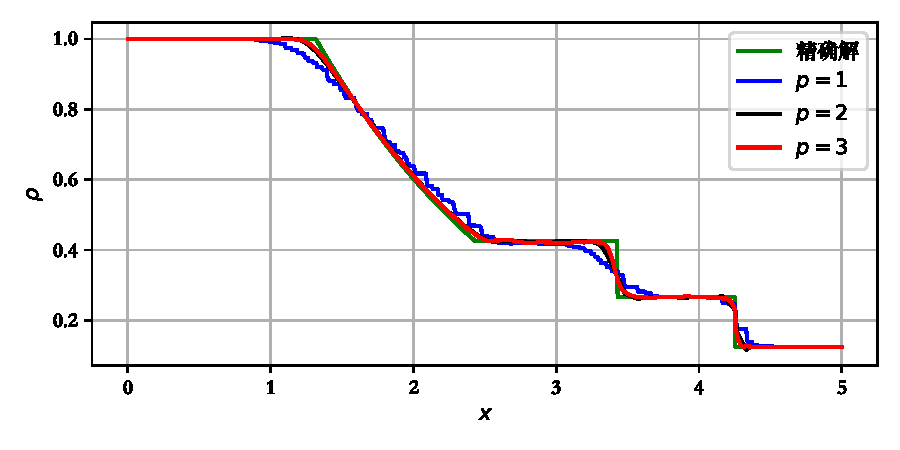
\includegraphics[width=1\textwidth,height=0.3\textheight]{figures/shock_tubes/sod/result_tetra}
\par\end{centering}
\caption{\label{fig:sod_tetra_p_vary}在只含 $h\approx0.1$ 的四面体单元的非结构网格上所得 \nameref{prob:Sod-=006FC0=006CE2=007BA1}问题
$\rho(x,y=0.5,z=0.25,t=1.0)$ 的各阶 RKDG 近似解之间的比较}
\end{figure}

为了更合理地比较不同阶数的求解器,作者开展了一组数值试验,将低阶 RKDG 求解器在细网格上的性能与高阶 RKDG 求解器在粗网格上的性能进行了对比。图
\ref{fig:sod_error}、表 \ref{tab:sod_cost} 给出了三组试验的结果。由该图、表可知:(1)
RK1/DG1 近似解的全局误差、运行时间、存储空间均最大,性价比最低;(2) RK3/DG3 与 RK3/DG3 近似解的全局误差、运行时间大致相当,但
RK2/DG2 近似解所需的存储空间较大,故其性价比低于 RK3/DG3 近似解;(3) 求解器精度每提高一阶,单元尺寸与时间步长可增加一倍,体单元数与时间步数的乘积可以减小为原来的
$1/16$。因此,只要 $p+1$ 阶 RKDG 求解器分摊到每个体单元上的单步计算量不超过 $p$ 阶 RKDG 求解器的
$16$ 倍,就具有更高的性价比。这里的“性”指全局精度,“价”指运行时间及存储空间。

\begin{figure}[h!]
\begin{centering}
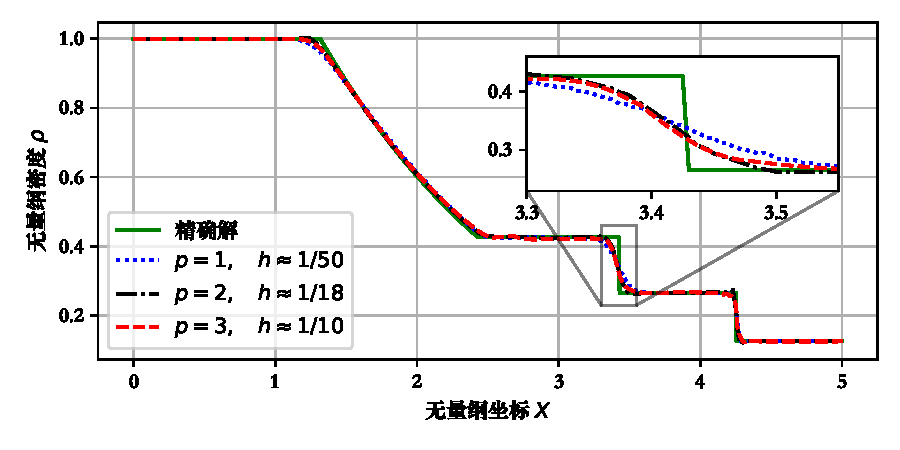
\includegraphics[width=1\textwidth,height=0.3\textheight]{figures/shock_tubes/sod/h_vary_tetra}
\par\end{centering}
\caption{\label{fig:sod_error}不同求解器–网格组合所得 \nameref{prob:Sod-=006FC0=006CE2=007BA1}问题
$\rho(x,y=0.5,z=0.25,t=1.0)$ 的计算精度之比较}
\end{figure}

\begin{table}
\caption{\label{tab:sod_cost}不同求解器–网格组合所得 \nameref{prob:Sod-=006FC0=006CE2=007BA1}问题的计算成本之比较}

\centering{}%
\begin{tabular}{cccccc}
\toprule 
$p$ & $h$ & 体单元数 & 时间步数 & 运行时间 (s) & 存储空间 (MB)\tabularnewline
\midrule 
1 & 1/50 & 2469675 & 1500 & 1492.16 & 1230\tabularnewline
2 & 1/18 & 117045 & 500 & 279.119 & 213\tabularnewline
3 & 1/10 & 19815 & 250 & 201.034 & 89\tabularnewline
\bottomrule
\end{tabular}
\end{table}

需要说明的是,不同于\nameref{prob:=007EBF=006027=005355=006CE2=005E73=006D41}问题所得的表
\ref{tab:linear_cost},表 \ref{tab:sod_cost} 中的数据没有夸大低阶 RKDG 求解器的运行时间,这是因为这里的
RK1/DG1、RK2/DG2 求解器采用了与之相对应的低阶数值积分器。具体地说,这里的 RK1/DG1 求解器采用了 1 点四面体积分器与
1 点三角形积分器,RK2/DG2 求解器采用了 4 点四面体积分器与 3 点三角形积分器,RK3/DG3 求解器采用了 14 点四面体积分器与
6 点三角形积分器。因此,本节关于性价比的结论比\nameref{prob:=007EBF=006027=005355=006CE2=005E73=006D41}问题所得的类似结论更加可靠,也更具有参考价值。

\subsection{Lax 激波管问题}
\begin{problem}
[Lax 激波管]\label{prob:Lax-=006FC0=006CE2=007BA1}在时间范围 $t\in[0.0,0.6]$
内,求满足三维欧拉方程 (\ref{eq:euler_system}) 及边界条件
\begin{equation}
\begin{bmatrix}\rho & u_{x} & u_{y} & u_{z} & p\end{bmatrix}=\begin{cases}
\begin{bmatrix}0.445 & 0.698 & 0.000 & 0.000 & 3.528\end{bmatrix}, & x=0,\\
\begin{bmatrix}0.500 & 0.000 & 0.000 & 0.000 & 0.571\end{bmatrix}, & x=5,
\end{cases}
\end{equation}
与初始条件

\begin{equation}
\begin{bmatrix}\rho & u_{x} & u_{y} & u_{z} & p\end{bmatrix}_{t=0}=\begin{cases}
\begin{bmatrix}\rho & u_{x} & u_{y} & u_{z} & p\end{bmatrix}_{x=0}, & x<2.5,\\
\begin{bmatrix}\rho & u_{x} & u_{y} & u_{z} & p\end{bmatrix}_{x=5}, & x>2.5,
\end{cases}
\end{equation}
的广义解。
\end{problem}

与 \nameref{prob:Sod-=006FC0=006CE2=007BA1}问题类似,该问题的精确解也含有激波、接触间断、膨胀波这三种间断。相对而言,该问题的求解难度更大,这是因为其精确解的各个分量均含有超出其初始值范围的部分,并且接触间断与激波的跳跃幅度远大于
\nameref{prob:Sod-=006FC0=006CE2=007BA1}问题中的值(无论是相对值还是绝对值)。

图 \ref{fig:lax_hexa} 给出了在只含 $h\approx0.1$ 的六面体单元的非结构网格上所得 \nameref{prob:Lax-=006FC0=006CE2=007BA1}问题的
RK3/DG3 近似解。

\begin{figure}[h!]
\begin{centering}
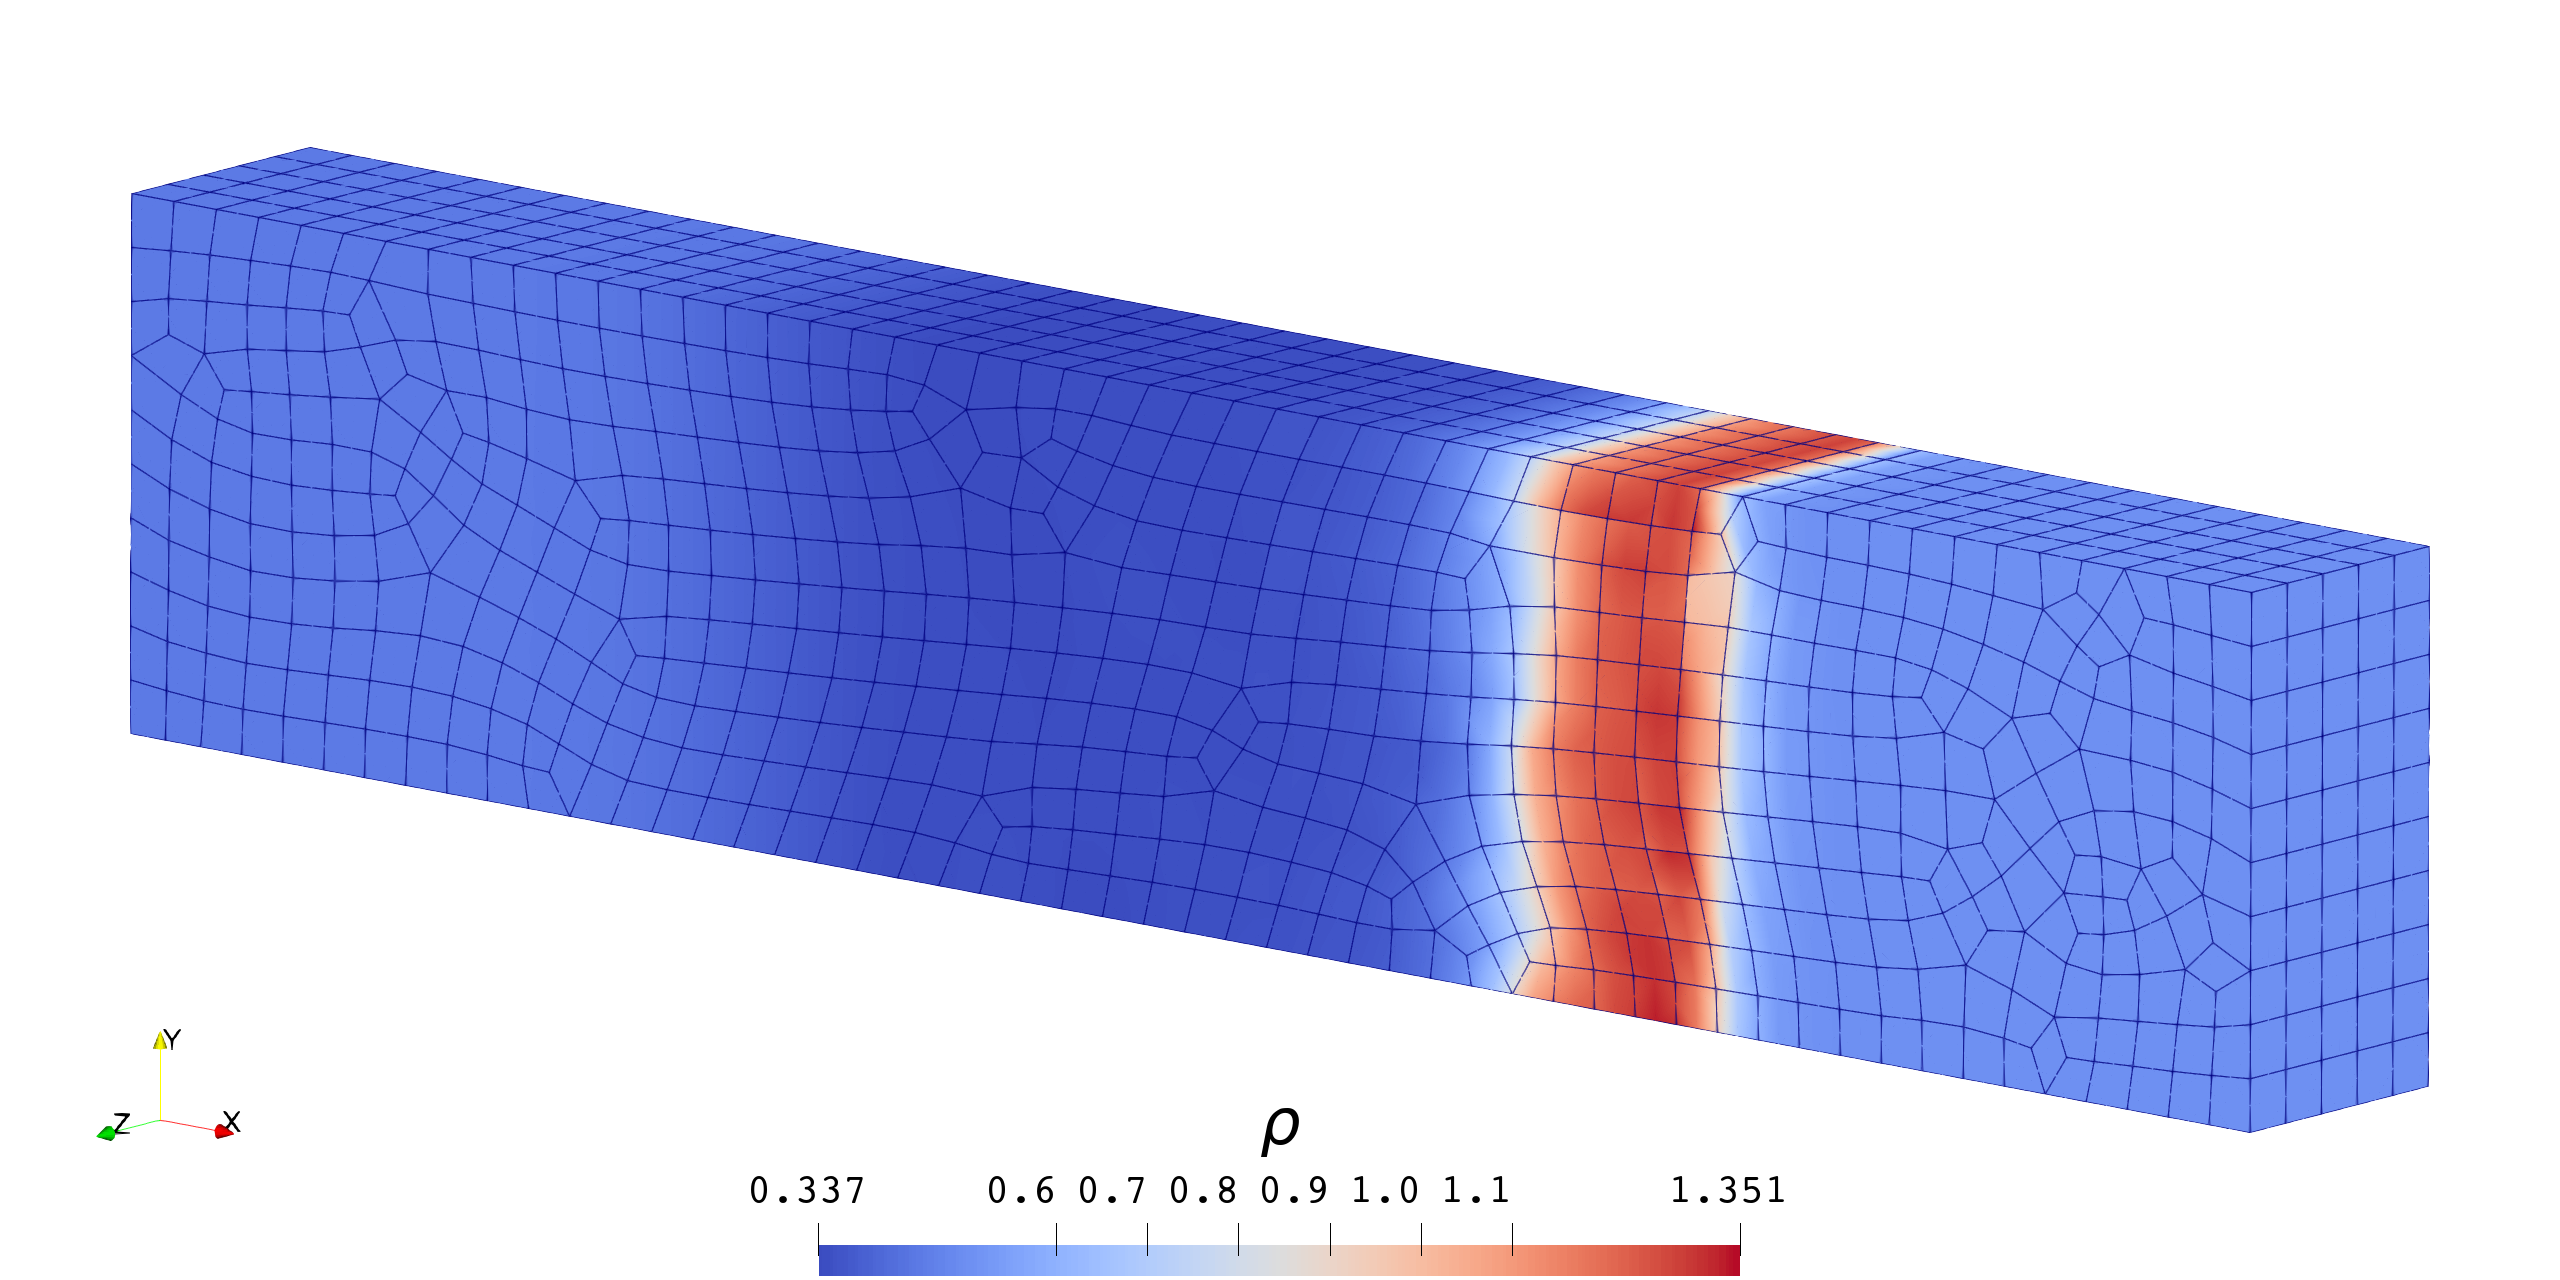
\includegraphics[width=1\textwidth]{../mdpi/figures/shock_tubes/lax/contour}
\par\end{centering}
\caption{\label{fig:lax_hexa}在只含 $h\approx0.1$ 的六面体单元的非结构网格上所得 \nameref{prob:Lax-=006FC0=006CE2=007BA1}问题
$\rho(x,y,z,t=0.5)$ 的 RK3/DG3 近似解}
\end{figure}

图 \ref{fig:lax_hexa_p_vary} 沿纵向对称轴 ($y=0.5,\,z=0.25$) 均匀选取了 1001
个采样点,依次画出了 RK1/DG1、RK2/DG2、RK3/DG3 近似解在这些采样点处的密度值。由这两幅图不难再次得出结论:(1)
高阶格式在间断附近引起的数值振荡得到了有效压制;(2) 在相同的网格上,求解器的阶数越高,数值解的精度也越高。

\begin{figure}[h!]
\begin{centering}
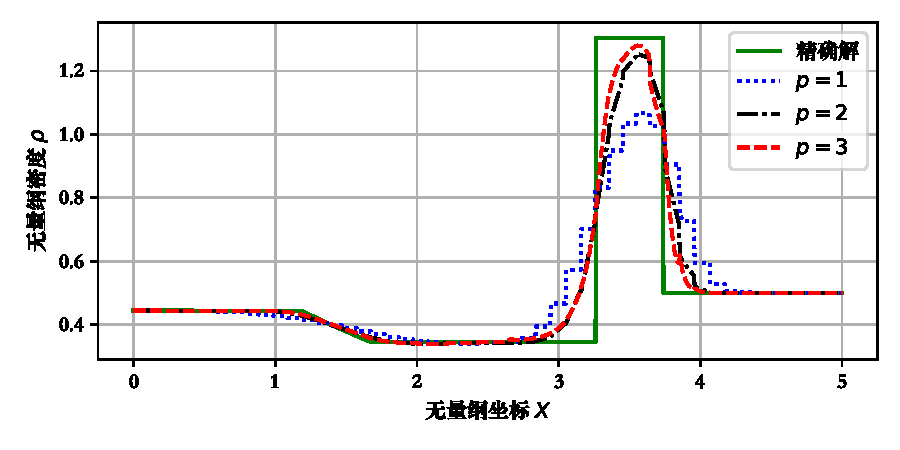
\includegraphics[width=1\textwidth,height=0.3\textheight]{figures/shock_tubes/lax/result}
\par\end{centering}
\caption{\label{fig:lax_hexa_p_vary}在只含 $h\approx0.1$ 的六面体单元的非结构网格上所得 \nameref{prob:Lax-=006FC0=006CE2=007BA1}问题
$\rho(x,y=0.5,z=0.25,t=0.5)$ 的各阶 RKDG 近似解之间的比较}
\end{figure}

为了验证计算结果及上述结论的网格无关性,我们在只含 $h\approx0.1$ 的四面体单元的非结构网格上再次求解了 \nameref{prob:Lax-=006FC0=006CE2=007BA1}问题,所得结果如图
\ref{fig:lax_tetra}、图 \ref{fig:lax_tetra_p_vary} 所示。

\begin{figure}[h!]
\begin{centering}
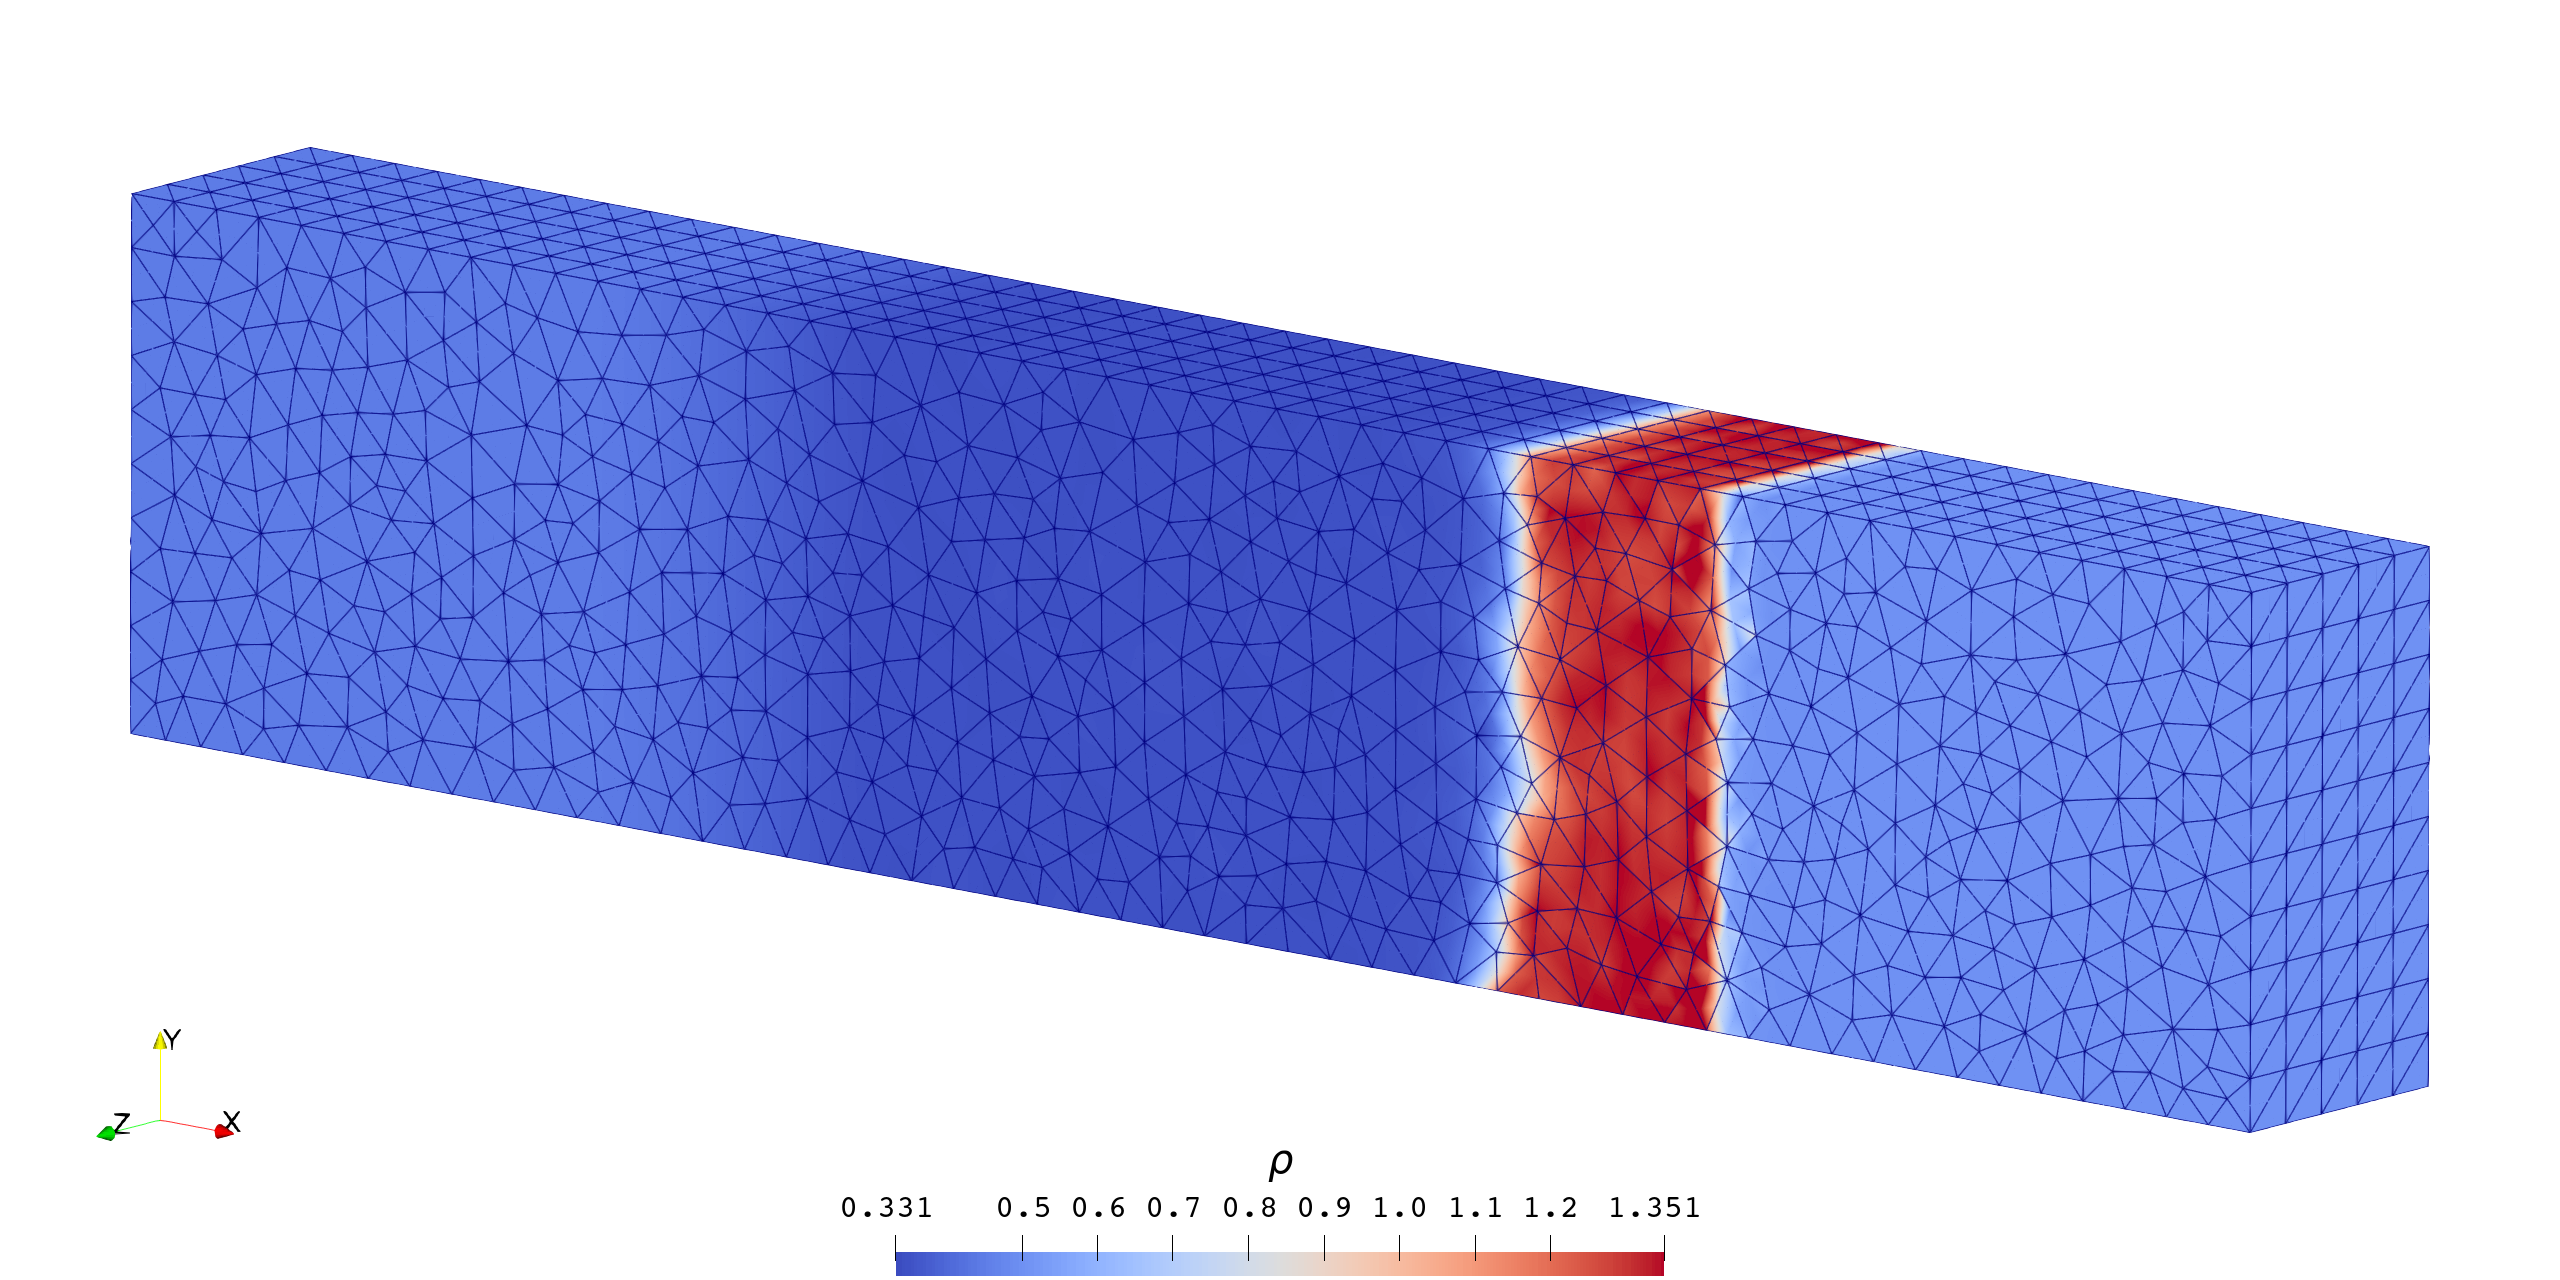
\includegraphics[width=1\textwidth]{../mdpi/figures/shock_tubes/lax/contour_tetra}
\par\end{centering}
\caption{\label{fig:lax_tetra}在只含 $h\approx0.1$ 的四面体单元的非结构网格上所得 \nameref{prob:Lax-=006FC0=006CE2=007BA1}问题
$\rho(x,y,z,t=0.5)$ 的 RK3/DG3 近似解}
\end{figure}

\begin{figure}[h!]
\begin{centering}
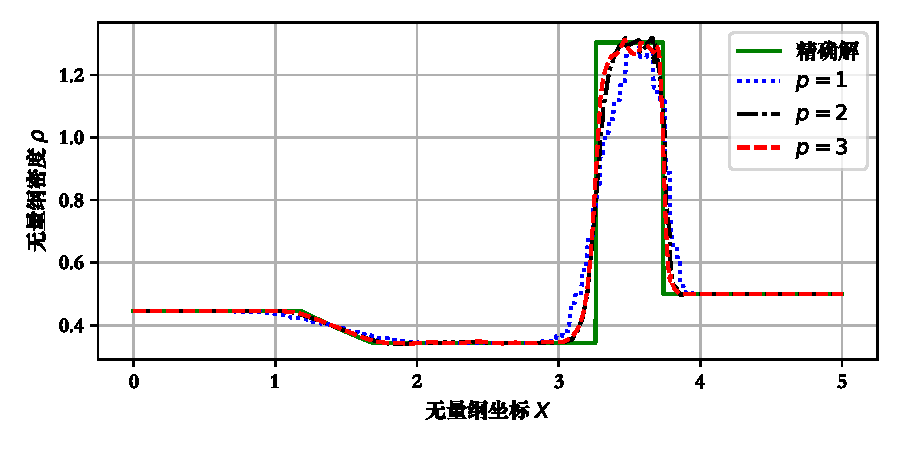
\includegraphics[width=1\textwidth,height=30cm,keepaspectratio]{figures/shock_tubes/lax/result_tetra}
\par\end{centering}
\caption{\label{fig:lax_tetra_p_vary}在只含 $h\approx0.1$ 的四面体单元的非结构网格上所得 \nameref{prob:Lax-=006FC0=006CE2=007BA1}问题
$\rho(x,y=0.5,z=0.25,t=0.5)$ 的各阶 RKDG 近似解之间的比较}
\end{figure}

将它们与图 \ref{fig:lax_hexa}–\ref{fig:lax_hexa_p_vary} 比较,不难发现:无论采用何种单元,只要网格足够精细,\nameref{prob:Lax-=006FC0=006CE2=007BA1}问题的各阶
RKDG 近似解均能收敛到精确解。

\subsection{真空管问题}
\begin{problem}
[真空管]\label{prob:=00771F=007A7A=007BA1}在时间范围 $t\in[0.0,0.4]$
内,求满足三维欧拉方程 (\ref{eq:euler_system}) 及边界条件
\begin{equation}
\begin{bmatrix}\rho & u_{x} & u_{y} & u_{z} & p\end{bmatrix}=\begin{cases}
\begin{bmatrix}1.0 & -4.0 & 0.0 & 0.0 & 0.4\end{bmatrix}, & x=0,\\
\begin{bmatrix}1.0 & +4.0 & 0.0 & 0.0 & 0.4\end{bmatrix}, & x=5,
\end{cases}
\end{equation}
与初始条件

\begin{equation}
\begin{bmatrix}\rho & u_{x} & u_{y} & u_{z} & p\end{bmatrix}_{t=0}=\begin{cases}
\begin{bmatrix}\rho & u_{x} & u_{y} & u_{z} & p\end{bmatrix}_{x=0}, & x<2.5,\\
\begin{bmatrix}\rho & u_{x} & u_{y} & u_{z} & p\end{bmatrix}_{x=5}, & x>2.5,
\end{cases}
\end{equation}
的广义解。
\end{problem}

该问题只含膨胀波这种导数值间断,不含激波、接触间断这类函数值间断,因此对限制器的要求比 \nameref{prob:Sod-=006FC0=006CE2=007BA1}问题及
\nameref{prob:Lax-=006FC0=006CE2=007BA1}问题更低。然而,该问题的精确解中含有一段连续的真空区域,这是求解前两个问题的过程中没有遇到过的现象。文献 \cite{Toro_2009}
的 4.6 节对真空区域的处理开展了充分的讨论。本文根据其建议,按如下方式确定真空区域的状态:真空区域(在下标中用 $*$ 表示)内没有气体分子,因此密度
$\rho$ 及压强 $p$ 可以设为 $0$,但速率 $u$ 是未定义的;另一方面,真空区域的边界恰好是膨胀波的波尾,因此其上的速率值可以由穿过膨胀波的黎曼不变量求得。

图 \ref{fig:vacuum_hexa} 给出了在只含 $h\approx0.1$ 的六面体单元的非结构网格上所得\nameref{prob:=00771F=007A7A=007BA1}问题的
RK3/DG3 近似解,图 \ref{fig:vacuum_hexa_p_vary} 沿纵向对称轴 ($y=0.5,\,z=0.25$)
均匀选取了 1001 个采样点,依次画出了 RK1/DG1、RK2/DG2、RK3/DG3 近似解在这些采样点处的密度值。结果再次验证了的有效性和阶数与精度的正相关。

\begin{figure}[h!]
\begin{centering}
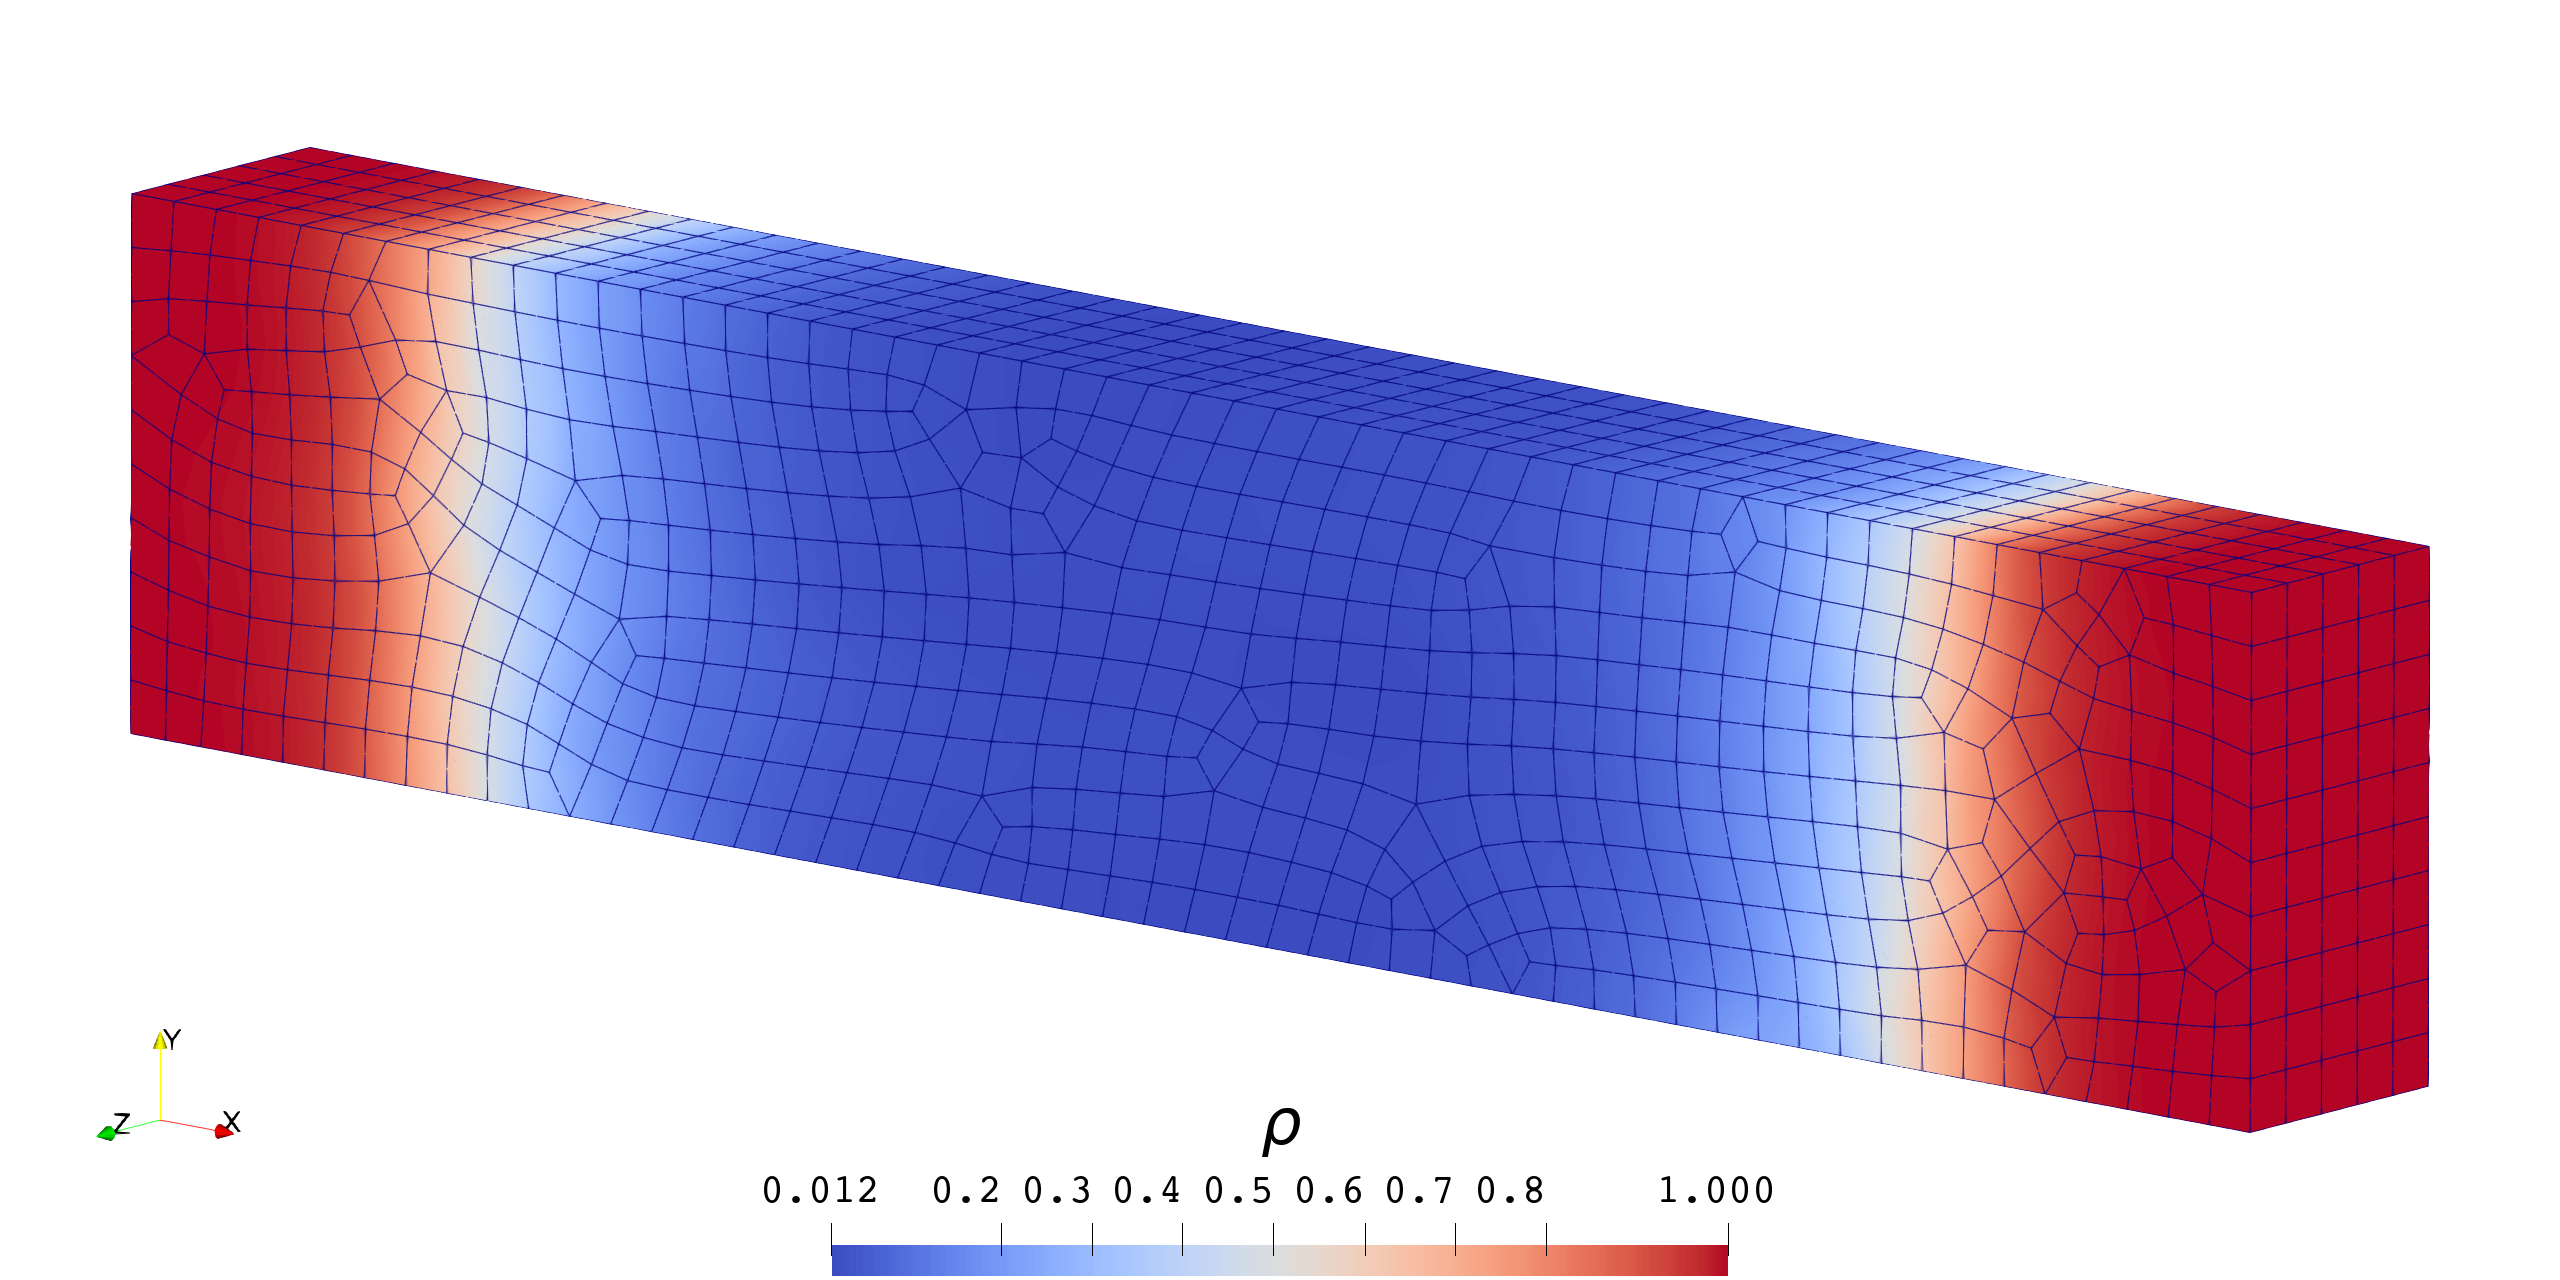
\includegraphics[width=0.98\textwidth]{../mdpi/figures/shock_tubes/vacuum/contour}
\par\end{centering}
\caption{\label{fig:vacuum_hexa}在只含 $h\approx0.1$ 的六面体单元的非结构网格上所得\nameref{prob:=00771F=007A7A=007BA1}问题
$\rho(x,y,z,t=0.4)$ 的 RK3/DG3 近似解}
\end{figure}

\begin{figure}[h!]
\begin{centering}
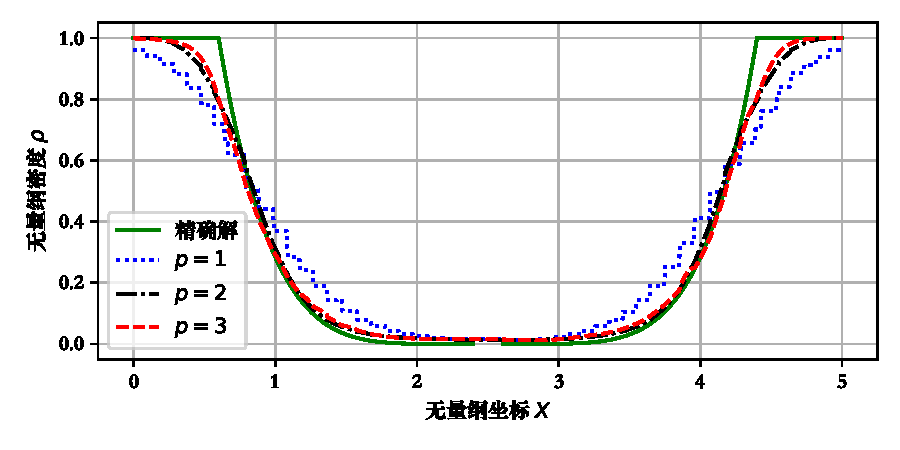
\includegraphics[width=1\textwidth,height=0.3\textheight,keepaspectratio]{figures/shock_tubes/vacuum/result}
\par\end{centering}
\caption{\label{fig:vacuum_hexa_p_vary}在只含 $h\approx0.1$ 的六面体单元的非结构网格上所得\nameref{prob:=00771F=007A7A=007BA1}问题
$\rho(x,y=0.5,z=0.25,t=0.4)$ 的各阶 RKDG 近似解之间的比较}
\end{figure}

与前两个问题类似,我们在只含 $h\approx0.1$ 的四面体单元的非结构网格上再次求解了\nameref{prob:=00771F=007A7A=007BA1}问题,所得结果如图
\ref{fig:vacuum_tetra}、图 \ref{fig:vacuum_tetra_p_vary} 所示。数值解的网格无关性再次得到了验证。

\begin{figure}[h!]
\begin{centering}
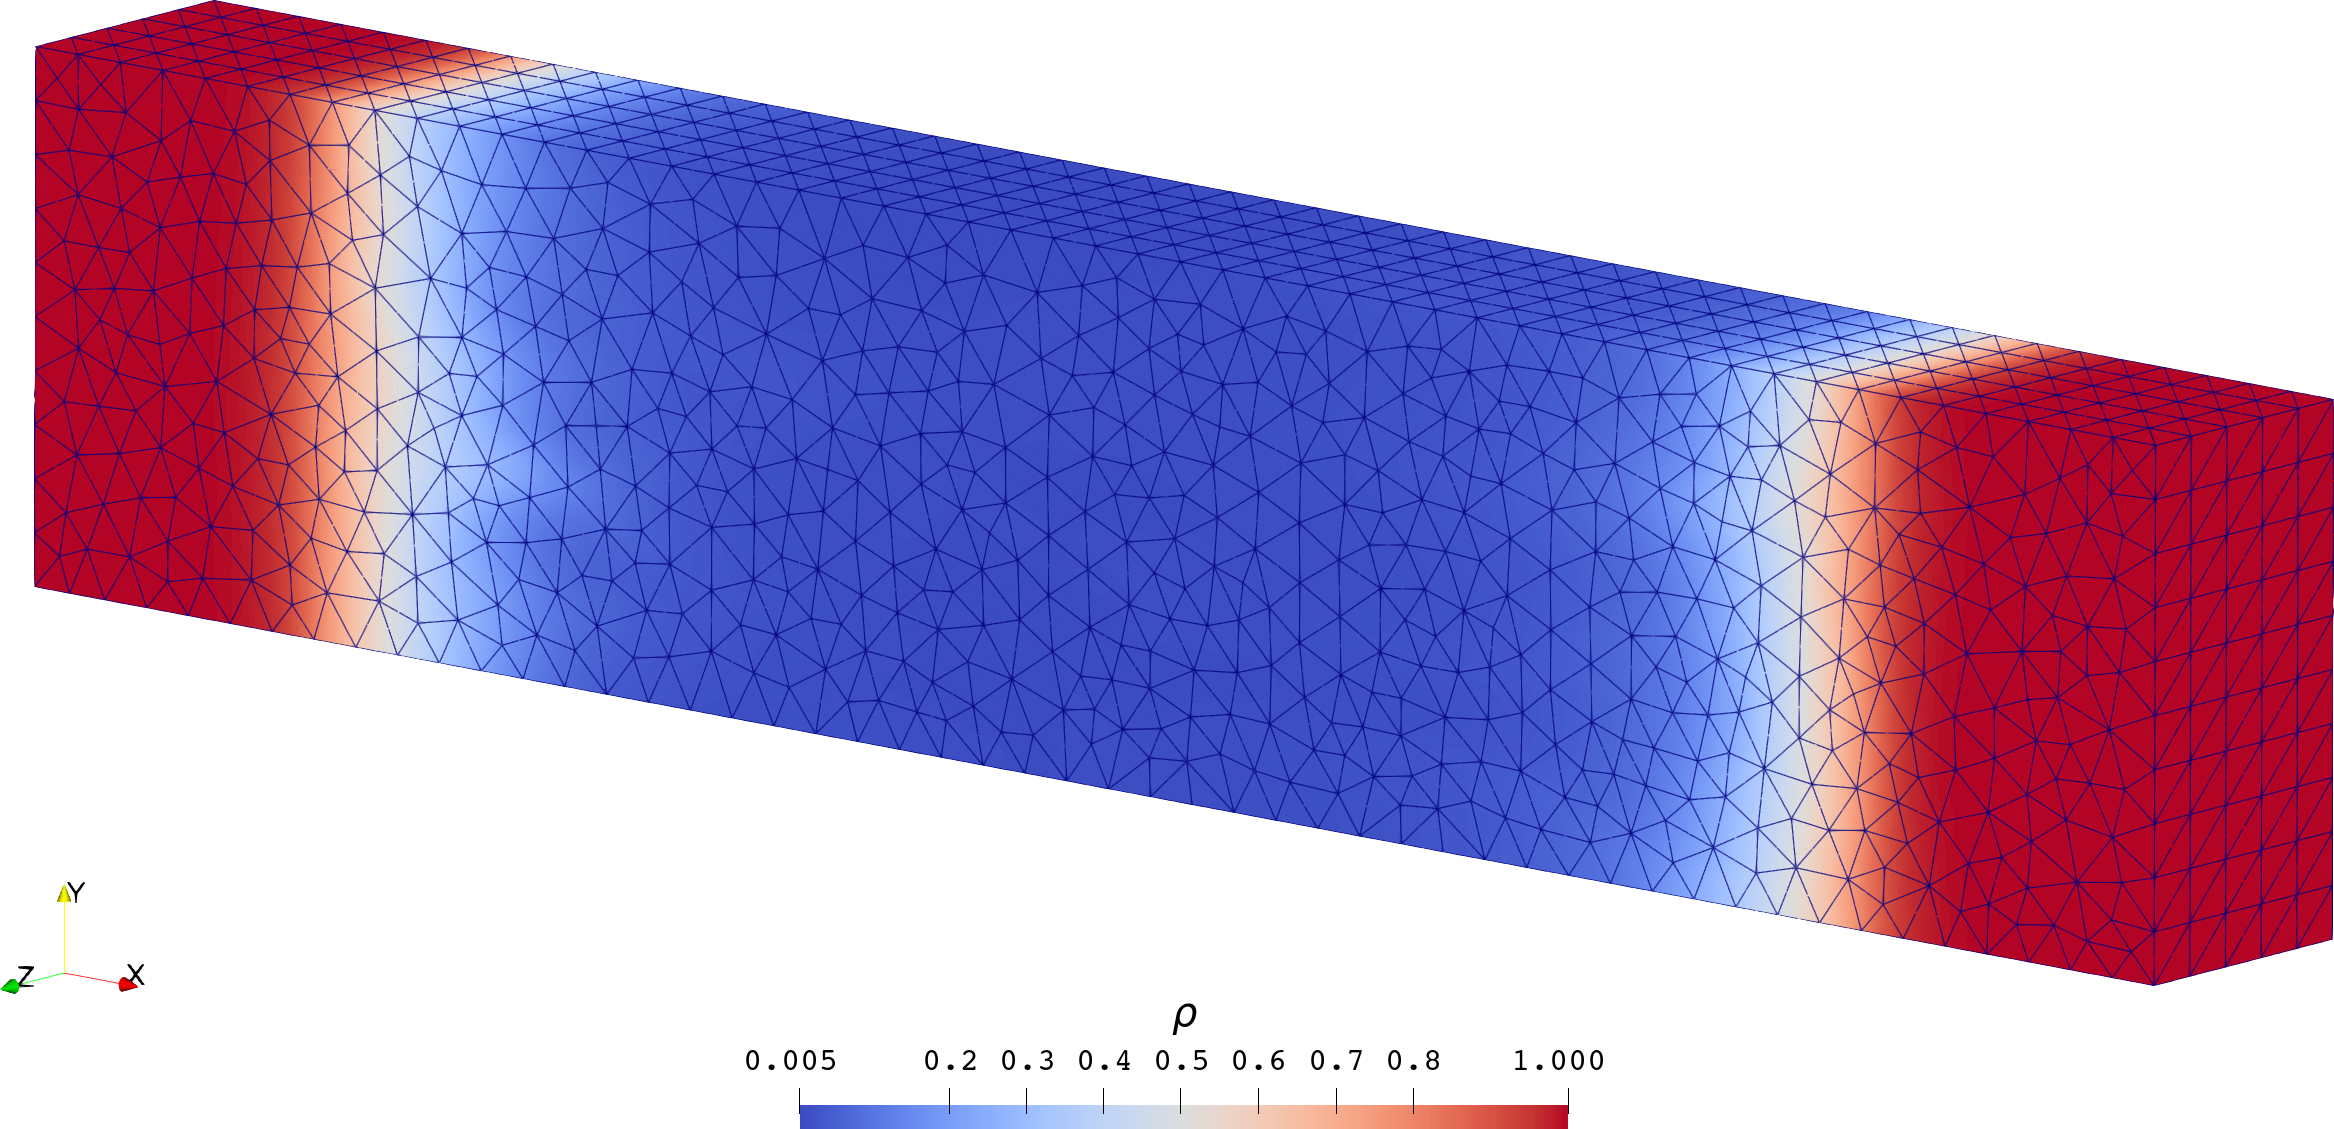
\includegraphics[width=0.98\textwidth]{../mdpi/figures/shock_tubes/vacuum/contour_tetra}
\par\end{centering}
\caption{\label{fig:vacuum_tetra}在只含 $h\approx0.1$ 的四面体单元的非结构网格上所得\nameref{prob:=00771F=007A7A=007BA1}问题
$\rho(x,y,z,t=0.4)$ 的 RK3/DG3 近似解}
\end{figure}

\begin{figure}[h!]
\begin{centering}
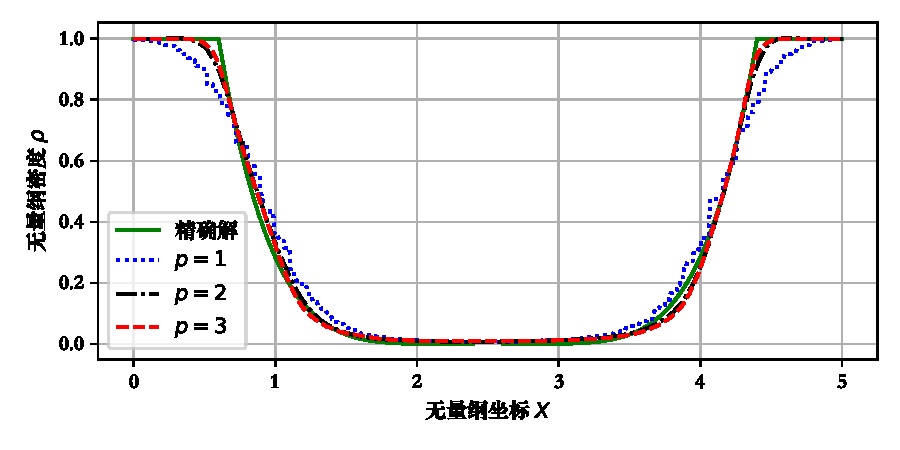
\includegraphics[width=1\textwidth,height=0.3\textheight,keepaspectratio]{figures/shock_tubes/vacuum/result_tetra}
\par\end{centering}
\caption{\label{fig:vacuum_tetra_p_vary}在只含 $h\approx0.1$ 的四面体单元的非结构网格上所得\nameref{prob:=00771F=007A7A=007BA1}问题
$\rho(x,y=0.5,z=0.25,t=0.4)$ 的各阶 RKDG 近似解之间的比较}
\end{figure}


\section{基于二维流场高精度近似解的定性验证}

\subsection{双马赫反射问题}

该问题模拟一道 $10$ 马赫的激波迎头撞击一个 $\ang{60}$ 楔形障碍物的流动图象,边界条件及初始条件如图 \ref{fig:double_mach_sketch}
所示,其中 $\delta=1/6$,黑色细实线表示固体壁面,红色粗实线表示初始激波。

\begin{figure}[h!]
\begin{centering}
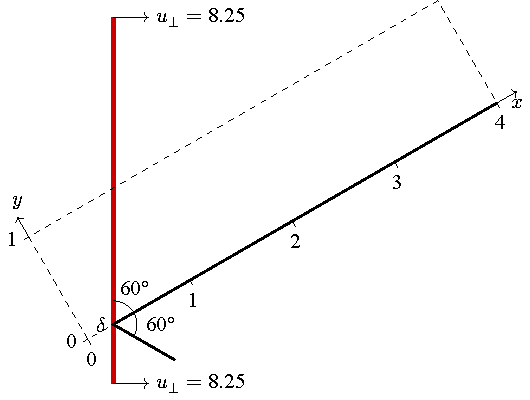
\includegraphics[width=1\textheight,height=0.33\textheight,keepaspectratio]{figures/double_mach/sketch}
\par\end{centering}
\caption{\label{fig:double_mach_sketch}\nameref{prob:=0053CC=009A6C=008D6B=0053CD=005C04}问题的边界条件及初始条件示意图}
\end{figure}

以文献 \cite{Woodward_1984} 为代表,该问题通常以二维形式出现。与激波管问题类似,本文在三维空间内重新给出其定义。
\begin{problem}
[双马赫反射]\label{prob:=0053CC=009A6C=008D6B=0053CD=005C04}在时间范围
$t\in[0.0,0.2]$ 及图 \ref{fig:double_mach_sketch} 中虚线所围计算区域(厚度 $Z$
为任意有限值)内,求满足三维欧拉方程 (\ref{eq:euler_system}) 及如下定解条件的广义解。

初始条件设为
\begin{equation}
\begin{bmatrix}\rho & u_{x} & u_{y} & u_{z} & p\end{bmatrix}_{t=0}=\begin{cases}
\begin{bmatrix}\rho & u_{x} & u_{y} & u_{z} & p\end{bmatrix}_{\mathrm{A}}, & \sqrt{3}(x-\delta)<y,\\
\begin{bmatrix}\rho & u_{x} & u_{y} & u_{z} & p\end{bmatrix}_{\mathrm{B}}, & \sqrt{3}(x-\delta)>y,
\end{cases}\label{eq:double_mach_ic}
\end{equation}
其中
\begin{equation}
\begin{aligned}\begin{bmatrix}\rho & u_{x} & u_{y} & u_{z} & p\end{bmatrix}_{\mathrm{A}} & =\begin{bmatrix}8.0 & 4.125\sqrt{3} & -4.125 & 0.0 & 116.5\end{bmatrix},\\
\begin{bmatrix}\rho & u_{x} & u_{y} & u_{z} & p\end{bmatrix}_{\mathrm{B}} & =\begin{bmatrix}1.4 & 0.0 & 0.0 & 0.0 & 1.0\end{bmatrix},
\end{aligned}
\end{equation}
分别为“波后 (After the wave)”与“波前 (Before the wave)”状态。

边界条件如下:
\begin{itemize}
\item 左端 ($x=0$) 为超声速入口,状态设为 $\begin{bmatrix}\rho & u_{x} & u_{y} & u_{z} & p\end{bmatrix}_{\mathrm{A}}$;
\item 右端 ($x=4$) 及底部前段 ($y=0$ 且 $x<\delta$) 为超声速出口(无需设置状态);
\item 底部后段 ($y=0$ 且 $x<\delta$) 为固体壁面;
\item 顶部 ($y=1$) 状态随时间变化,并且与初始条件 (\ref{eq:double_mach_ic}) 兼容:
\begin{equation}
\begin{bmatrix}\rho & u_{x} & u_{y} & u_{z} & p\end{bmatrix}=\begin{cases}
\begin{bmatrix}\rho & u_{x} & u_{y} & u_{z} & p\end{bmatrix}_{\mathrm{A}}, & x-(\delta+u_{x,\mathrm{A}}t)<\sqrt{\frac{1}{3}},\\
\begin{bmatrix}\rho & u_{x} & u_{y} & u_{z} & p\end{bmatrix}_{\mathrm{B}}, & x-(\delta+u_{x,\mathrm{A}}t)>\sqrt{\frac{1}{3}}.
\end{cases}\qedhere
\end{equation}
\end{itemize}
\end{problem}

该问题的解具有自相似性,因此只需要画出某一时刻的计算结果。图 \ref{fig:double_mach_p=00003D1_h=00003D5e-3}–\ref{fig:double_mach_p=00003D3_h=00003D5e-3}
依次为\nameref{prob:=0053CC=009A6C=008D6B=0053CD=005C04}问题在只含 $h\approx1/200$
的六面体单元的非结构网格上的 RK1/DG1、RK2/DG2、RK3/DG3 近似解。

\begin{figure}[h!]
\begin{centering}
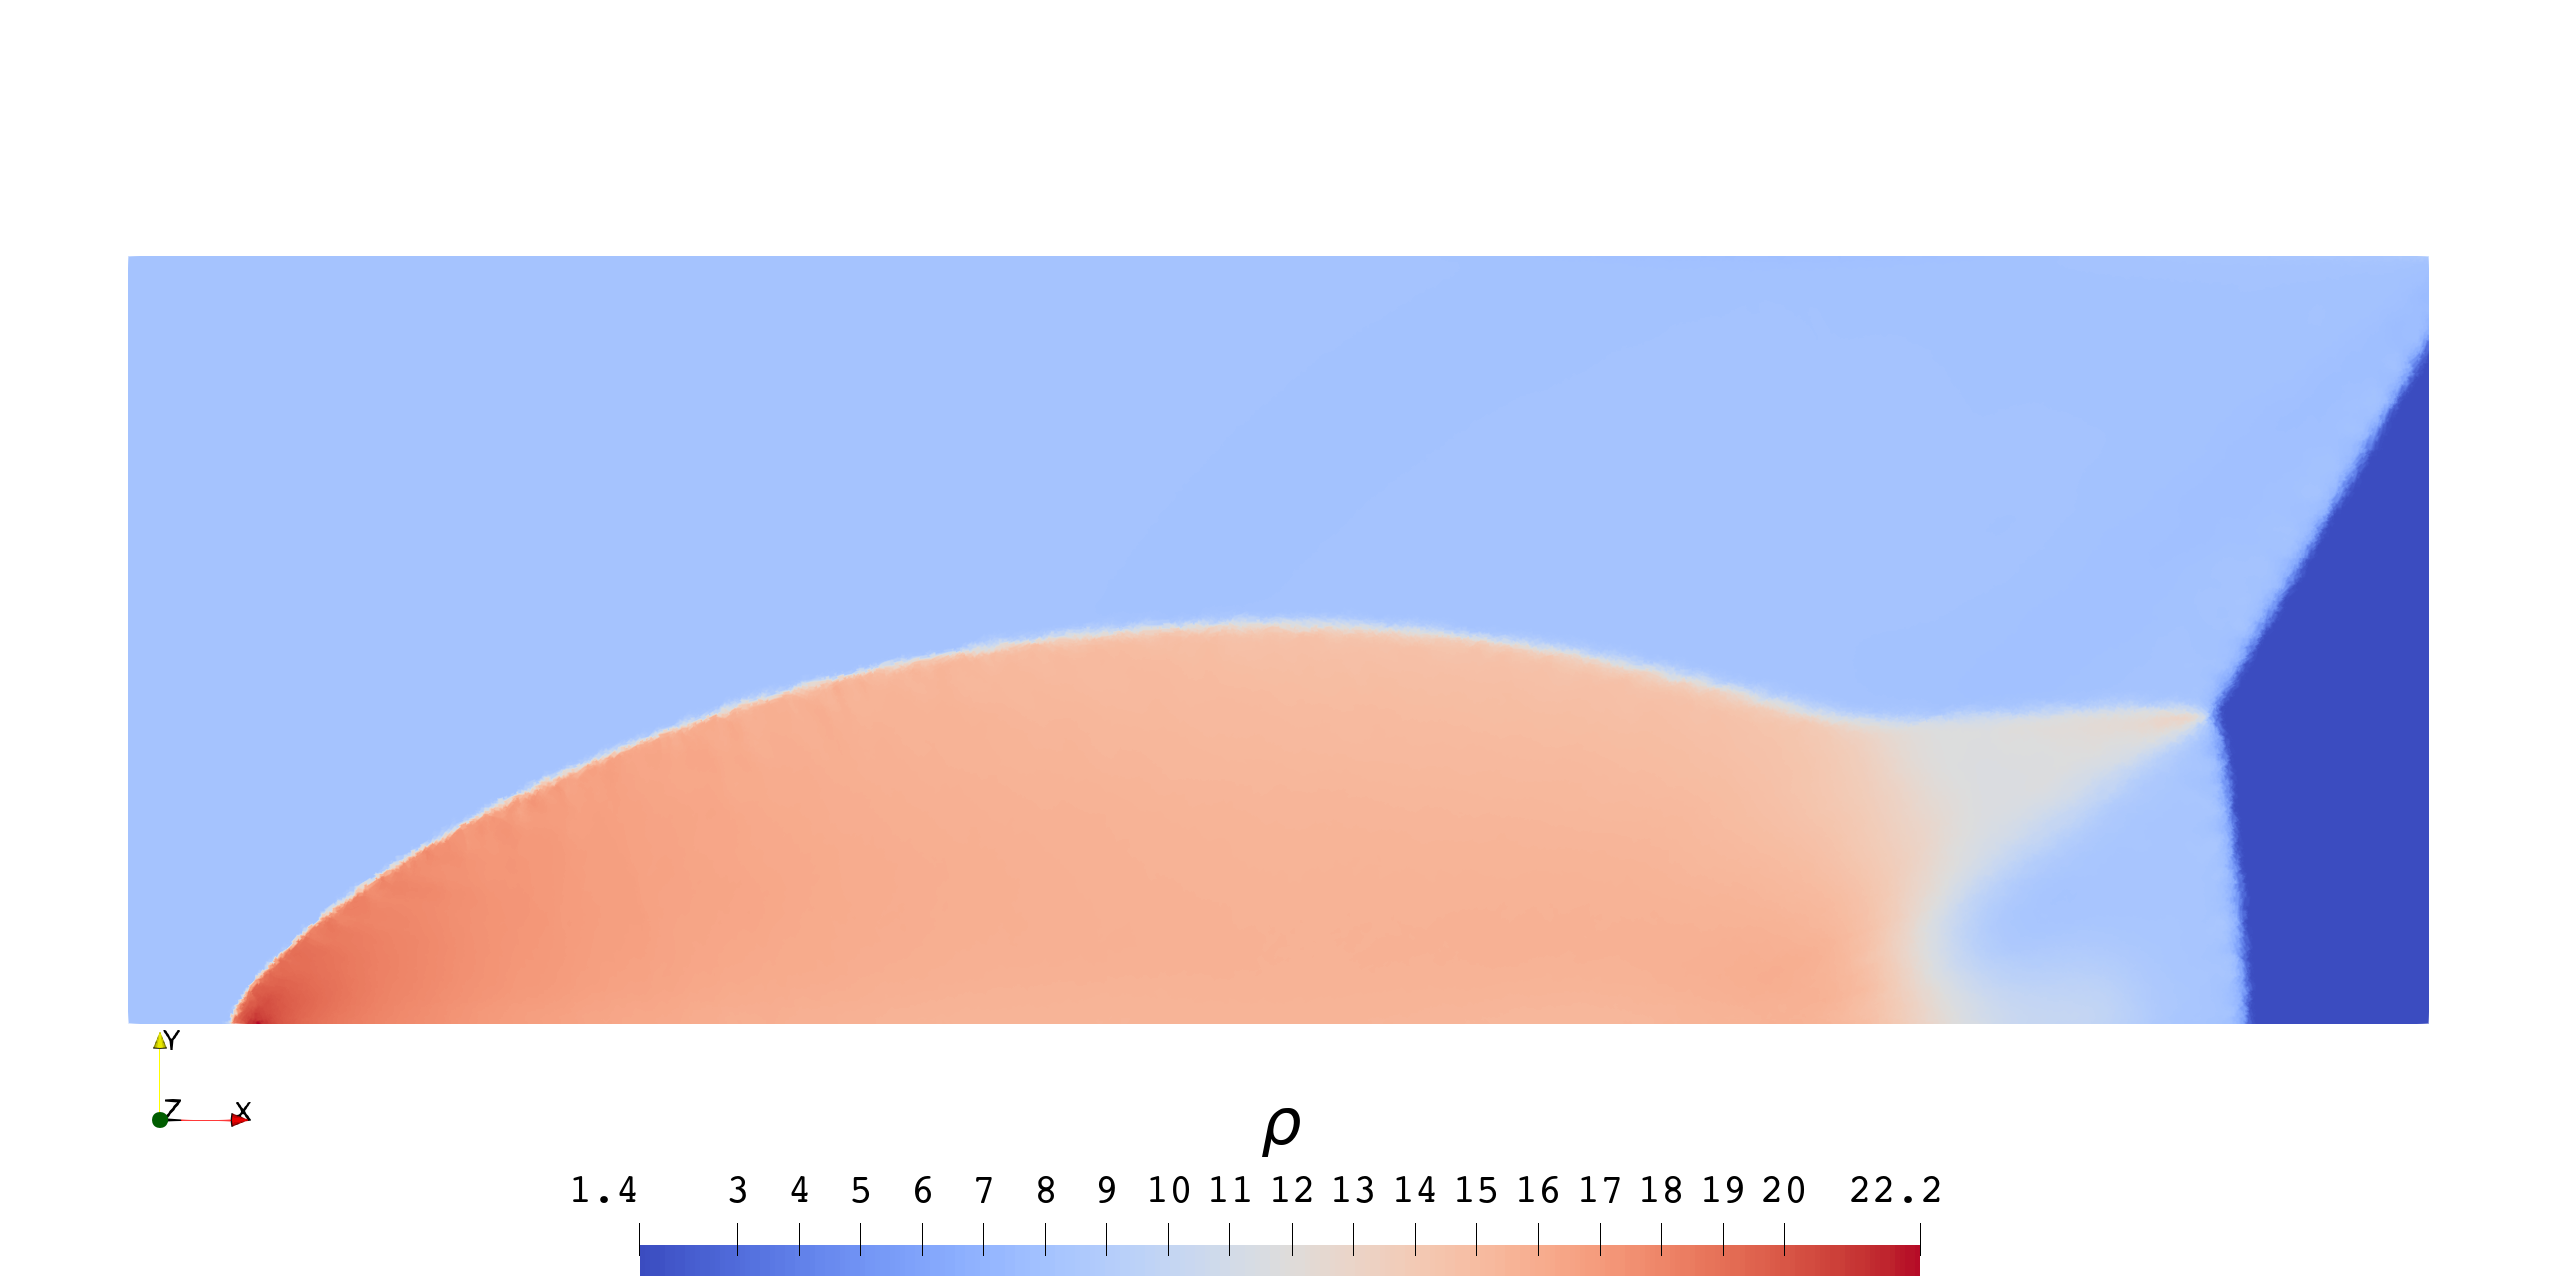
\includegraphics[width=1\textwidth]{../mdpi/figures/double_mach/p=1_h=5e-3}
\par\end{centering}
\caption{\label{fig:double_mach_p=00003D1_h=00003D5e-3}在只含 $h\approx1/200$
的六面体单元的非结构网格上所得\nameref{prob:=0053CC=009A6C=008D6B=0053CD=005C04}问题
$\rho(x,y,z=Z/2,t=0.2)$ 的 RK1/DG1 近似解}
\end{figure}

\begin{figure}[h!]
\begin{centering}
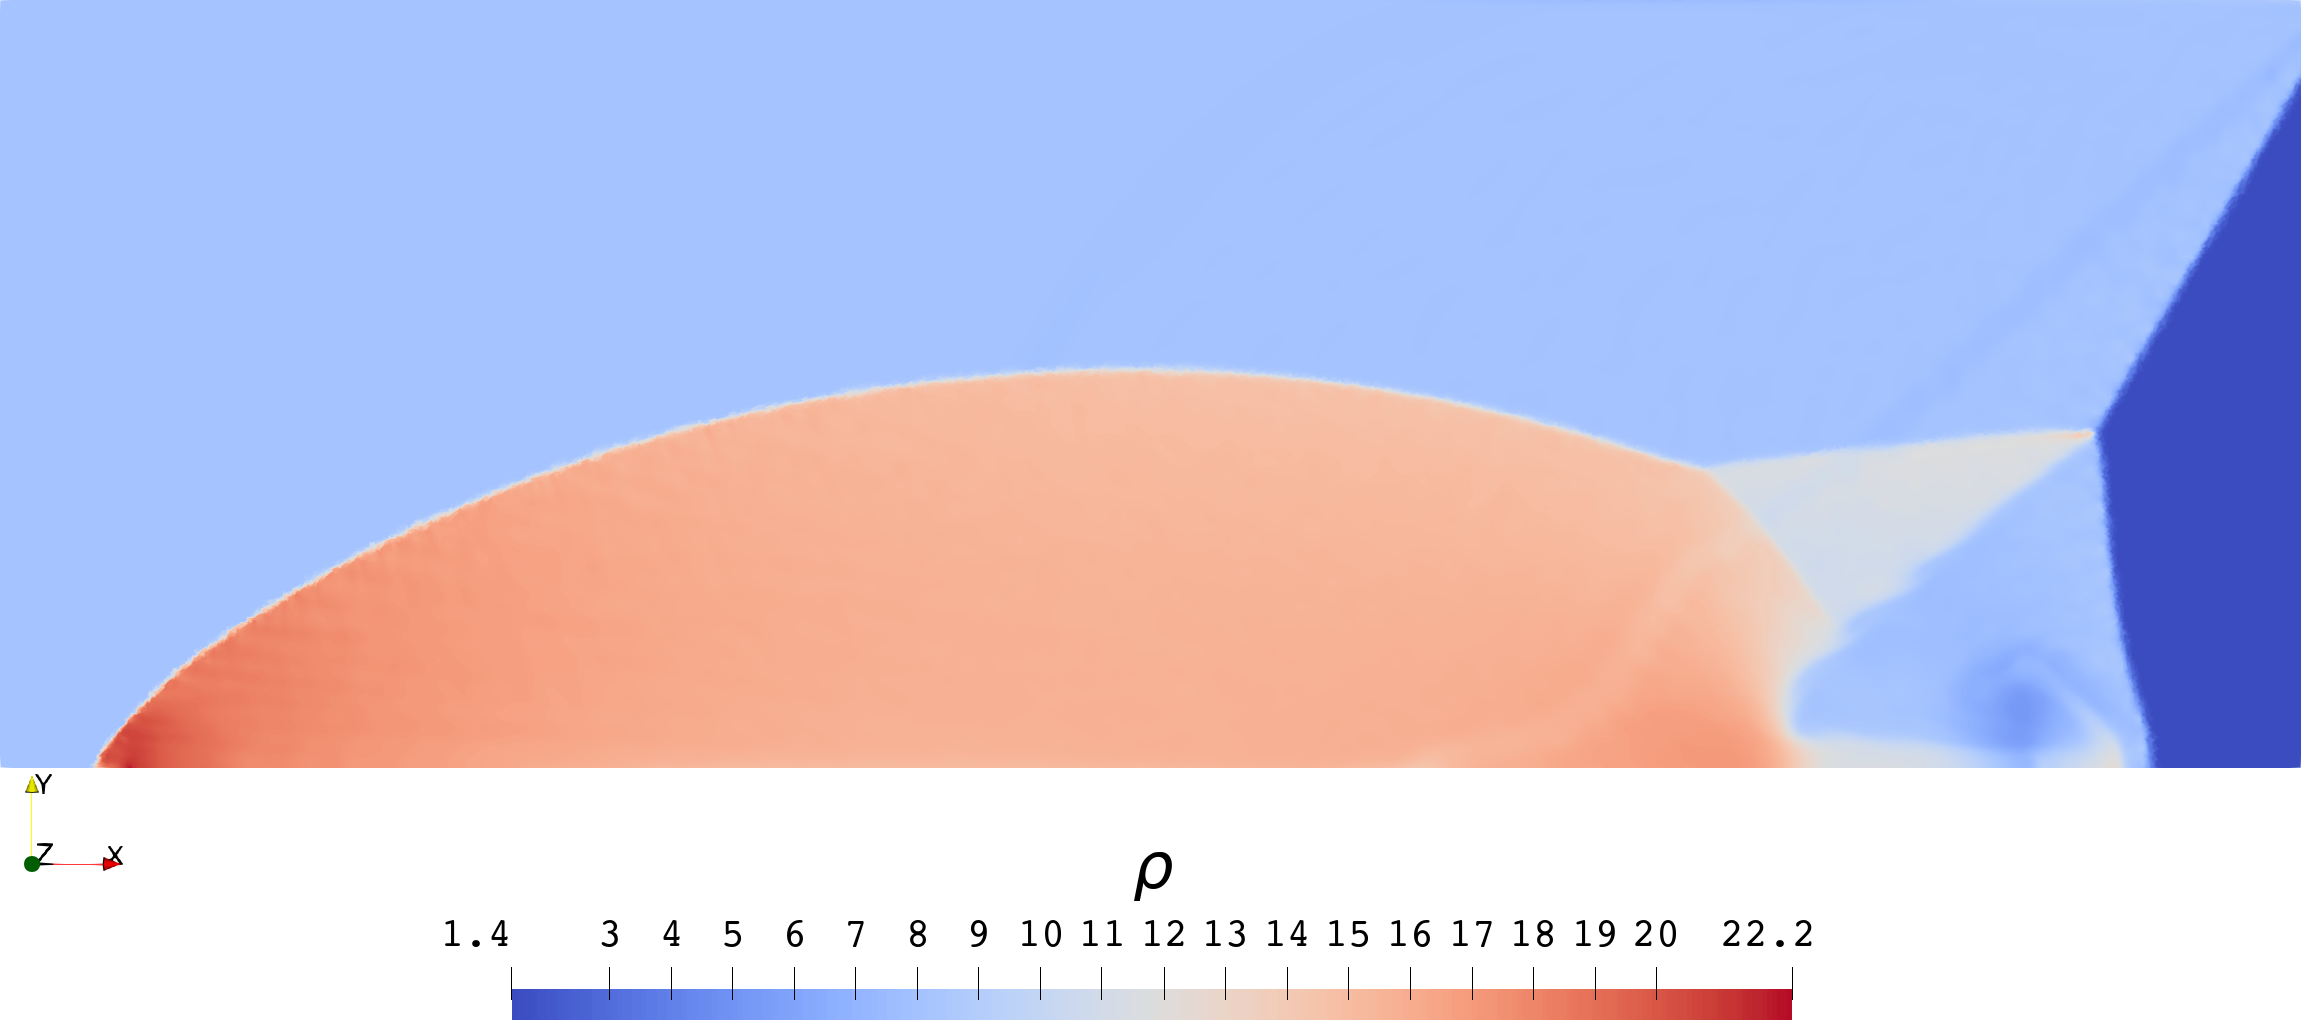
\includegraphics[width=1\textwidth]{../mdpi/figures/double_mach/p=2_h=5e-3}
\par\end{centering}
\caption{\label{fig:double_mach_p=00003D2_h=00003D5e-3}在只含 $h\approx1/200$
的六面体单元的非结构网格上所得\nameref{prob:=0053CC=009A6C=008D6B=0053CD=005C04}问题
$\rho(x,y,z=Z/2,t=0.2)$ 的 RK2/DG2 近似解}
\end{figure}

\begin{figure}[h!]
\begin{centering}
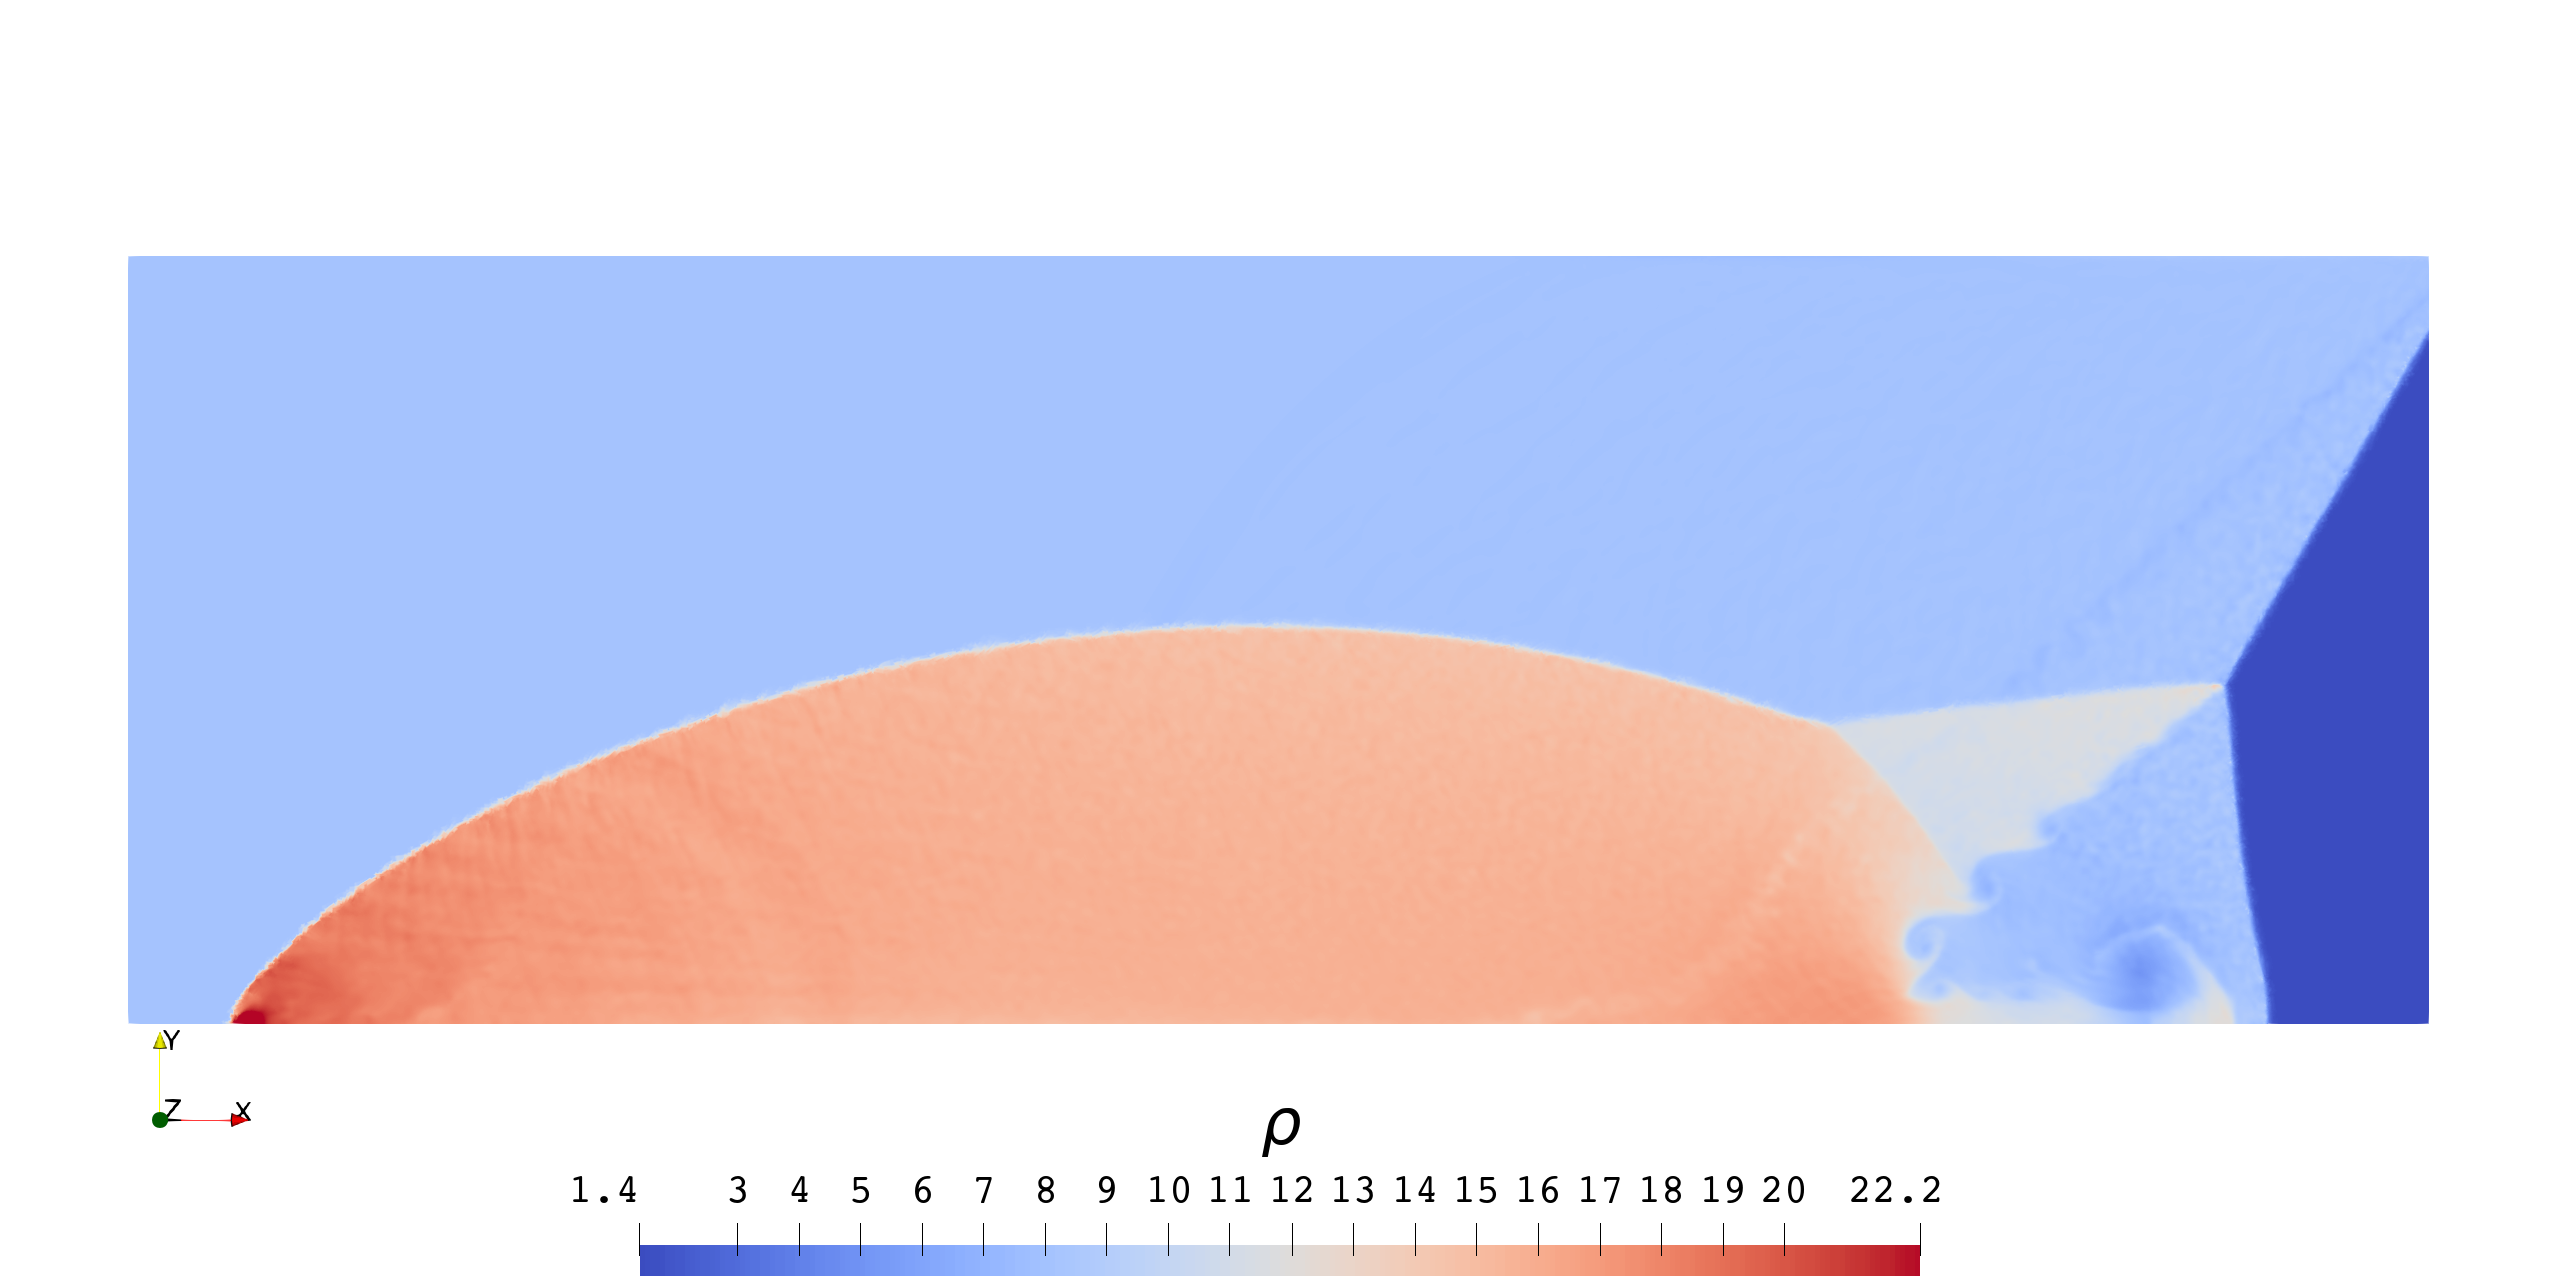
\includegraphics[width=1\textwidth]{../mdpi/figures/double_mach/p=3_h=5e-3}
\par\end{centering}
\caption{\label{fig:double_mach_p=00003D3_h=00003D5e-3}在只含 $h\approx1/200$
的六面体单元的非结构网格上所得\nameref{prob:=0053CC=009A6C=008D6B=0053CD=005C04}问题
$\rho(x,y,z=Z/2,t=0.2)$ 的 RK3/DG3 近似解}
\end{figure}

三者给出的流场结构大致相同,都含有一道弓形激波与两组马赫反射;但只有高阶近似解才能捕捉到右下角的复杂涡系。这种差别再次体现了高阶 RKDG
求解器分辨流动细节的优越性。

为了定性验证以上结果的正确性,图 \ref{fig:double_mach_p=00003D3_zhong} 给出了文献 \cite{Zhong_2013}
在 $h=1/240$ 的二维结构网格上所得二维 RK3/DG3 近似解。将其与图 \ref{fig:double_mach_p=00003D3_h=00003D5e-3}
即本文在 $h\approx1/200$ 的三维非结构网格上所得三维 RK3/DG3 近似解对比,不难发现:二者给出的流场结构几乎完全一致,这说明本文所实现的三维
RK3/DG3 求解器能够在三维非结构网格上正确地捕捉复杂的二维流场结构。

\begin{figure}[h!]
\begin{centering}
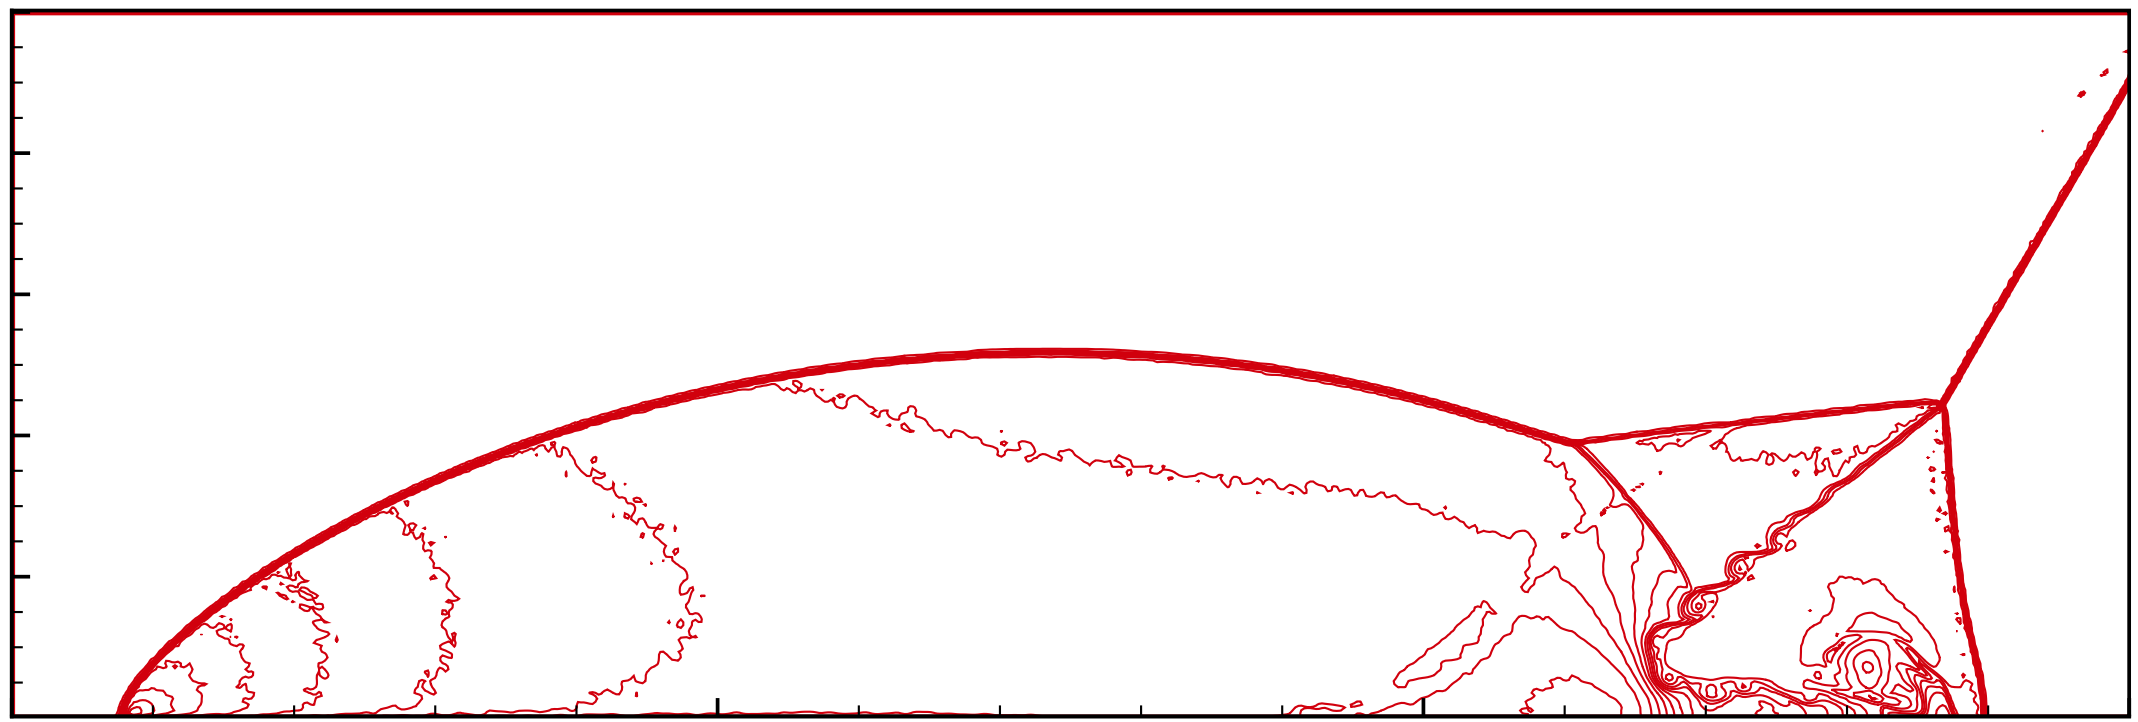
\includegraphics[width=1\textwidth]{figures/double_mach/zhong}
\par\end{centering}
\caption{\label{fig:double_mach_p=00003D3_zhong}在只含 $h=1/240$ 的四边形单元的二维结构网格上所得\nameref{prob:=0053CC=009A6C=008D6B=0053CD=005C04}问题
$\rho(x,y,t=0.2)$ 的 RK3/DG3 近似解\upcite{Zhong_2013}}
\end{figure}


\subsection{前向台阶问题}

该问题是另一个用于校验无黏可压缩气流数值解的经典二维问题。该问题的边界条件与初始条件比双马赫反射问题的简单,但其解不具有自相似性,所涉及的物理现象更加复杂,因此对求解器的性能要求更为苛刻。与双马赫反射问题类似,我们在三维空间内重新给出其定义。
\begin{problem}
[前向台阶]\label{prob:=00524D=005411=0053F0=009636}考虑一个由三维区间
$[0,3]\times[0,1]\times[0,Z]$ 表示的风洞,其底部设有一始于 $x=0.6$ 处、高度为 $0.2$
的水平台阶。左端 ($x=0$) 为超声速入口,右端 ($x=3$) 为超声速出口,其余边界均设为固体壁面。在上述计算区域与时间范围
$t\in[0.0,4.0]$ 内,求满足三维欧拉方程 (\ref{eq:euler_system}) 及初始条件
\begin{equation}
\begin{bmatrix}\rho & u_{x} & u_{y} & u_{z} & p\end{bmatrix}_{t=0}=\begin{bmatrix}1.4 & 3.0 & 0.0 & 0.0 & 1.0\end{bmatrix}
\end{equation}
与边界条件
\begin{equation}
\begin{bmatrix}\rho & u_{x} & u_{y} & u_{z} & p\end{bmatrix}_{x=0}=\begin{bmatrix}\rho & u_{x} & u_{y} & u_{z} & p\end{bmatrix}_{t=0}
\end{equation}
的广义解。
\end{problem}

图 \ref{fig:forward_step_domain} 给出了一种可用于求解该问题的只含有 $h=1/20$ 的六面体单元的伪结构网格。这里的“伪结构”指其可以用结构网格的数据结构来表示,但本小节的所有算例仍将其以非结构网格的数据结构来表示。需要说明的是,该网格仅用于展示网格拓扑,其精细程度不足以捕捉图
\ref{fig:forward_step_p=00003D3_t=00003D02e-1}–\ref{fig:forward_step_p=00003D3_t=00003D40e-1}
所示的复杂流动结构。实际上,图 \ref{fig:forward_step_p=00003D3_t=00003D02e-1}–\ref{fig:forward_step_p=00003D3_t=00003D40e-1}
使用了 $h=1/200$ 的精细网格。

\begin{figure}[h!]
\begin{centering}
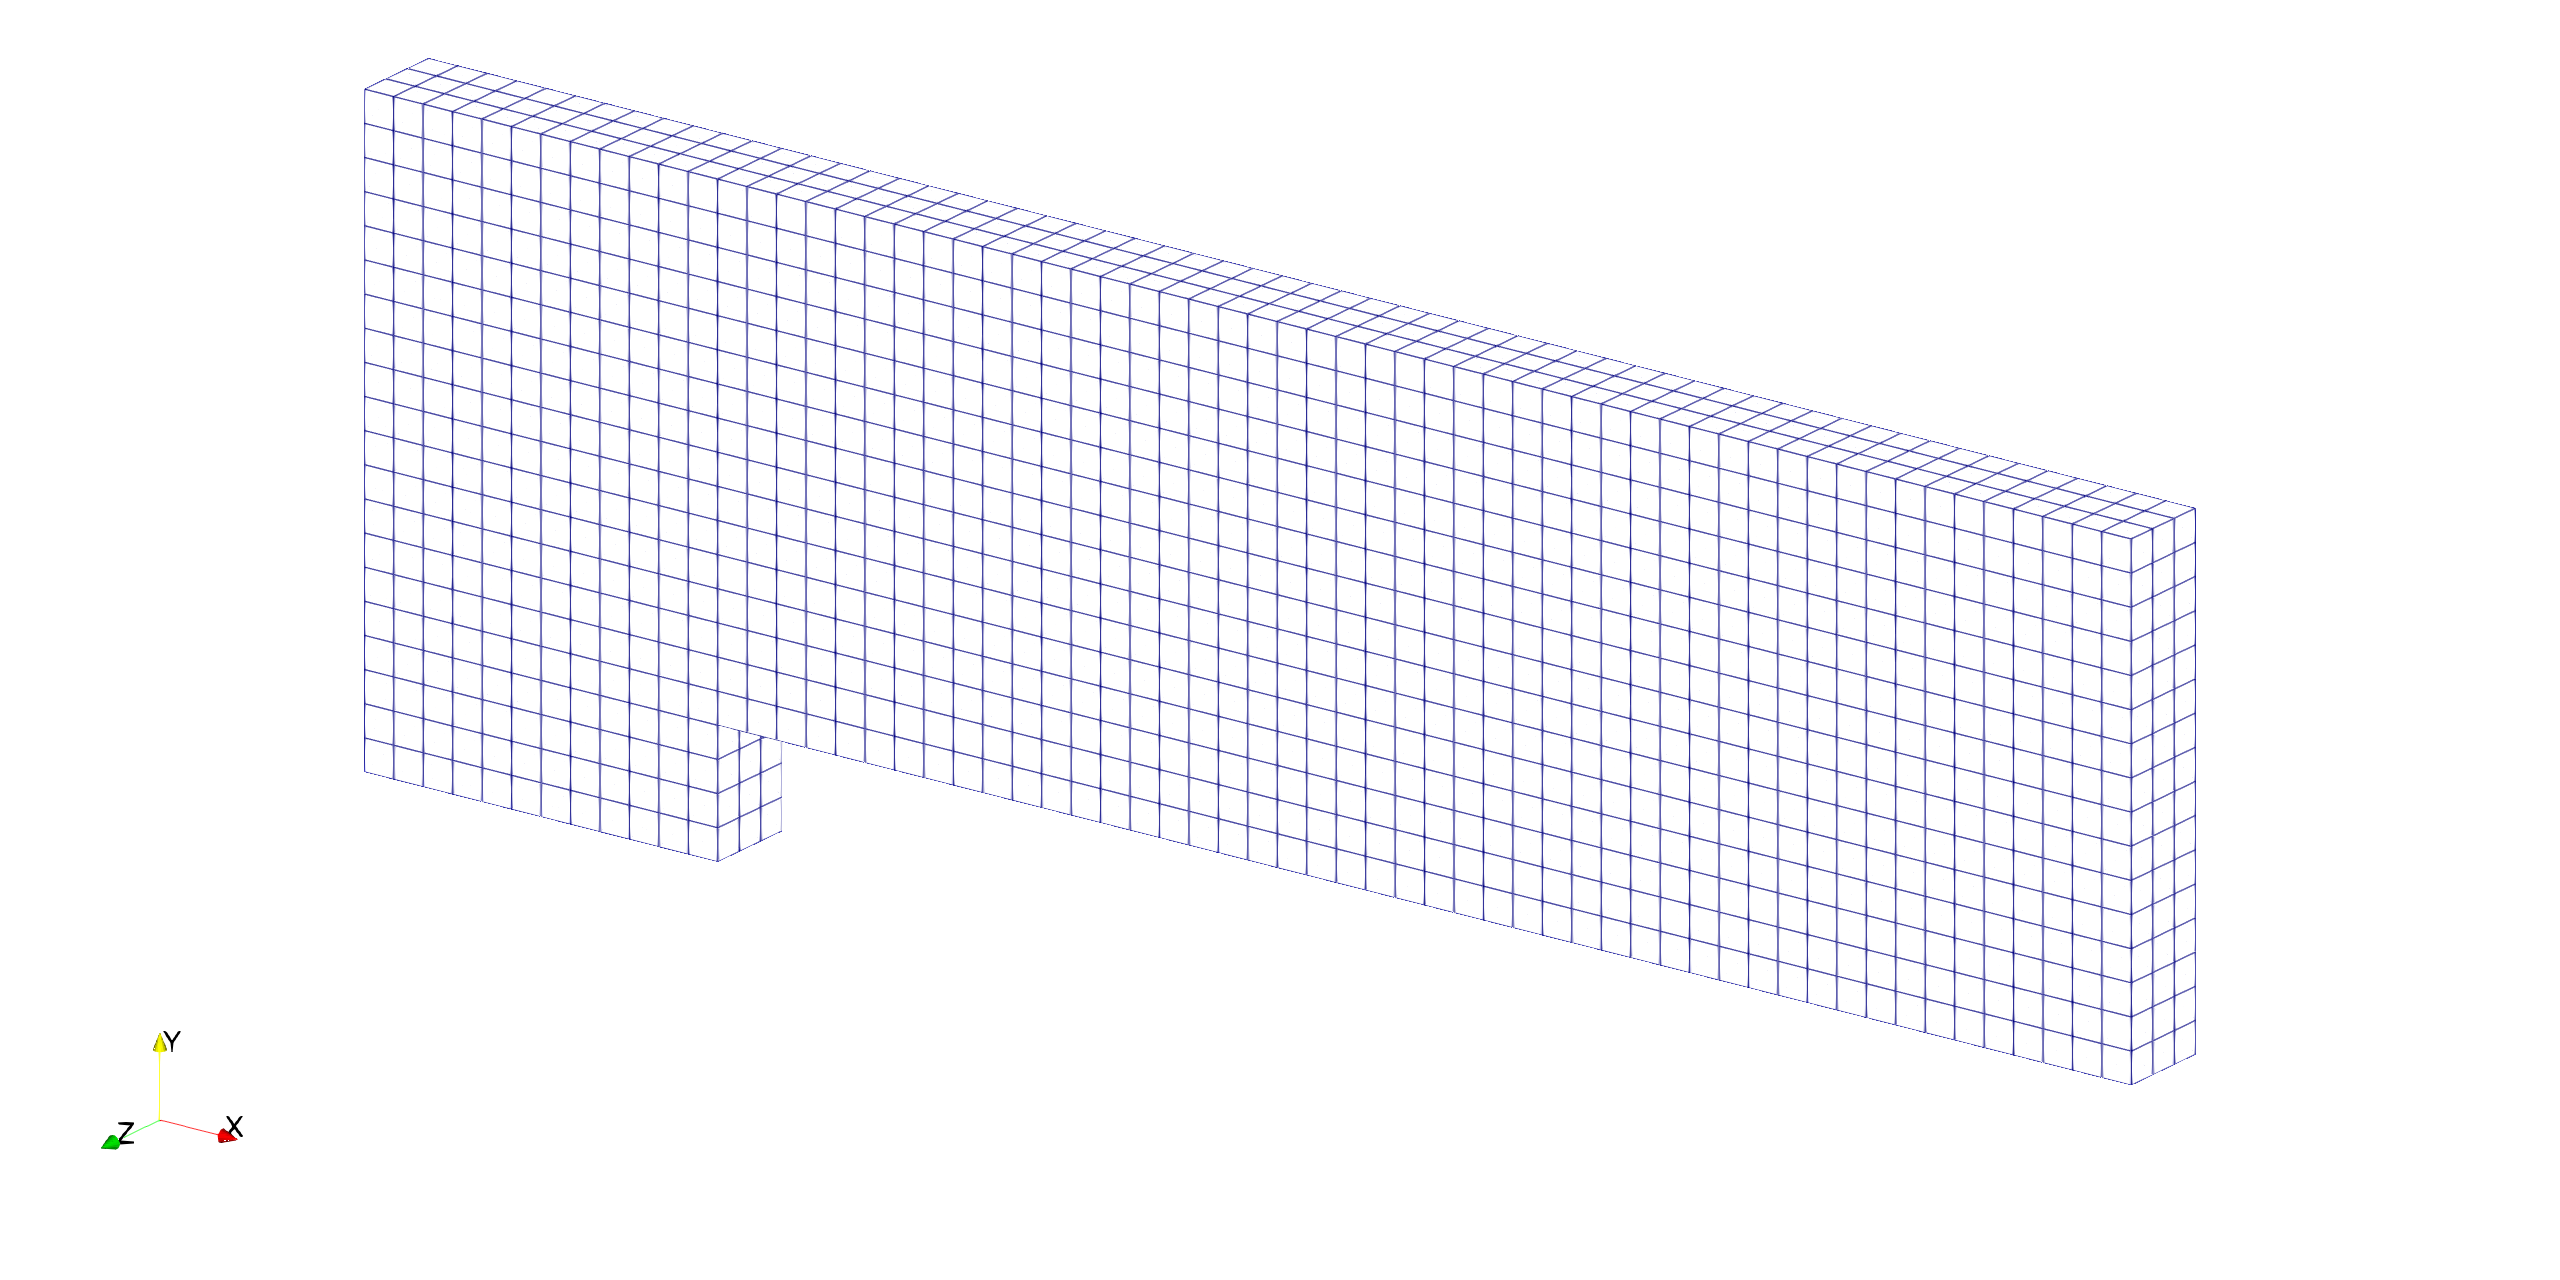
\includegraphics[width=1\textwidth,height=0.26\textheight,keepaspectratio]{../mdpi/figures/forward_step/mesh}
\par\end{centering}
\caption{\label{fig:forward_step_domain}用于求解\nameref{prob:=00524D=005411=0053F0=009636}问题的只含
$h=1/20$ 的六面体单元的伪结构网格}
\end{figure}

由于该问题的解在上述时间范围内剧烈变化,最理想的呈现计算结果的方式应当是动画。本节仿照文献 \cite{Woodward_1984}
的做法,将数值解在若干时刻的状态分别以图片的形式给出。

流场始于 $3$ 马赫的均匀状态。

计时开始后,超声速气流撞击在台阶上,形成一道弓形激波,如图 \ref{fig:forward_step_p=00003D3_t=00003D02e-1}、图
\ref{fig:forward_step_p=00003D3_t=00003D04e-1} 所示。与此同时,在台阶上表面前端的拐角处
($x=0.6$, $y=0.2$) 还形成了一道膨胀波,拐角附近的气流状态接近真空。因此该算例对求解器捕捉激波和处理真空的能力都提出了很高的要求。

\begin{figure}[h!]
\begin{centering}
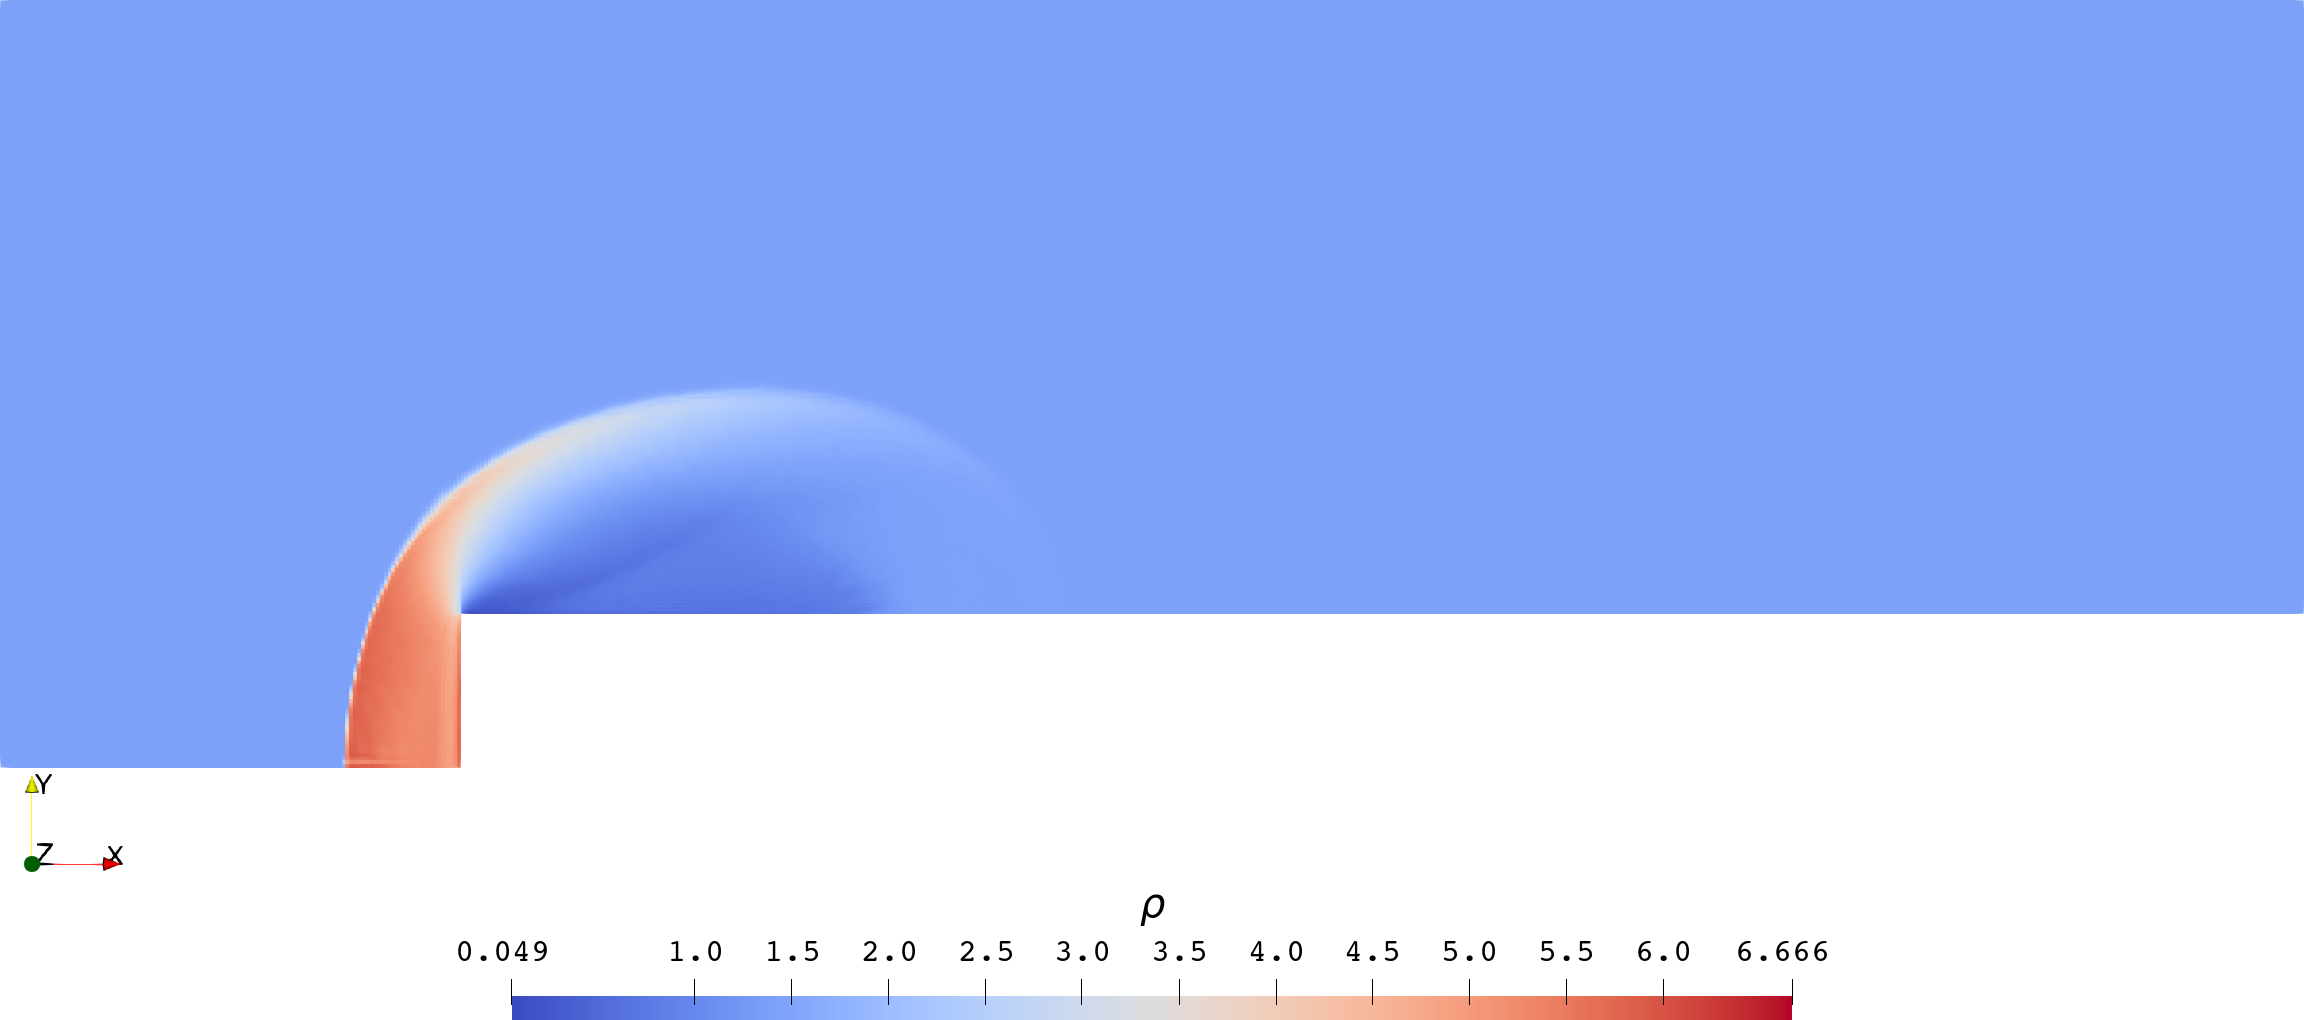
\includegraphics[width=1\textwidth,height=0.28\textheight]{../mdpi/figures/forward_step/p=3_t=02e-1}
\par\end{centering}
\caption{\label{fig:forward_step_p=00003D3_t=00003D02e-1}在 $h=1/200$ 的伪结构网格上所得\nameref{prob:=00524D=005411=0053F0=009636}问题在
$t=0.2$ 时刻的 RK3/DG3 近似解}
\end{figure}

\begin{figure}[h!]
\begin{centering}
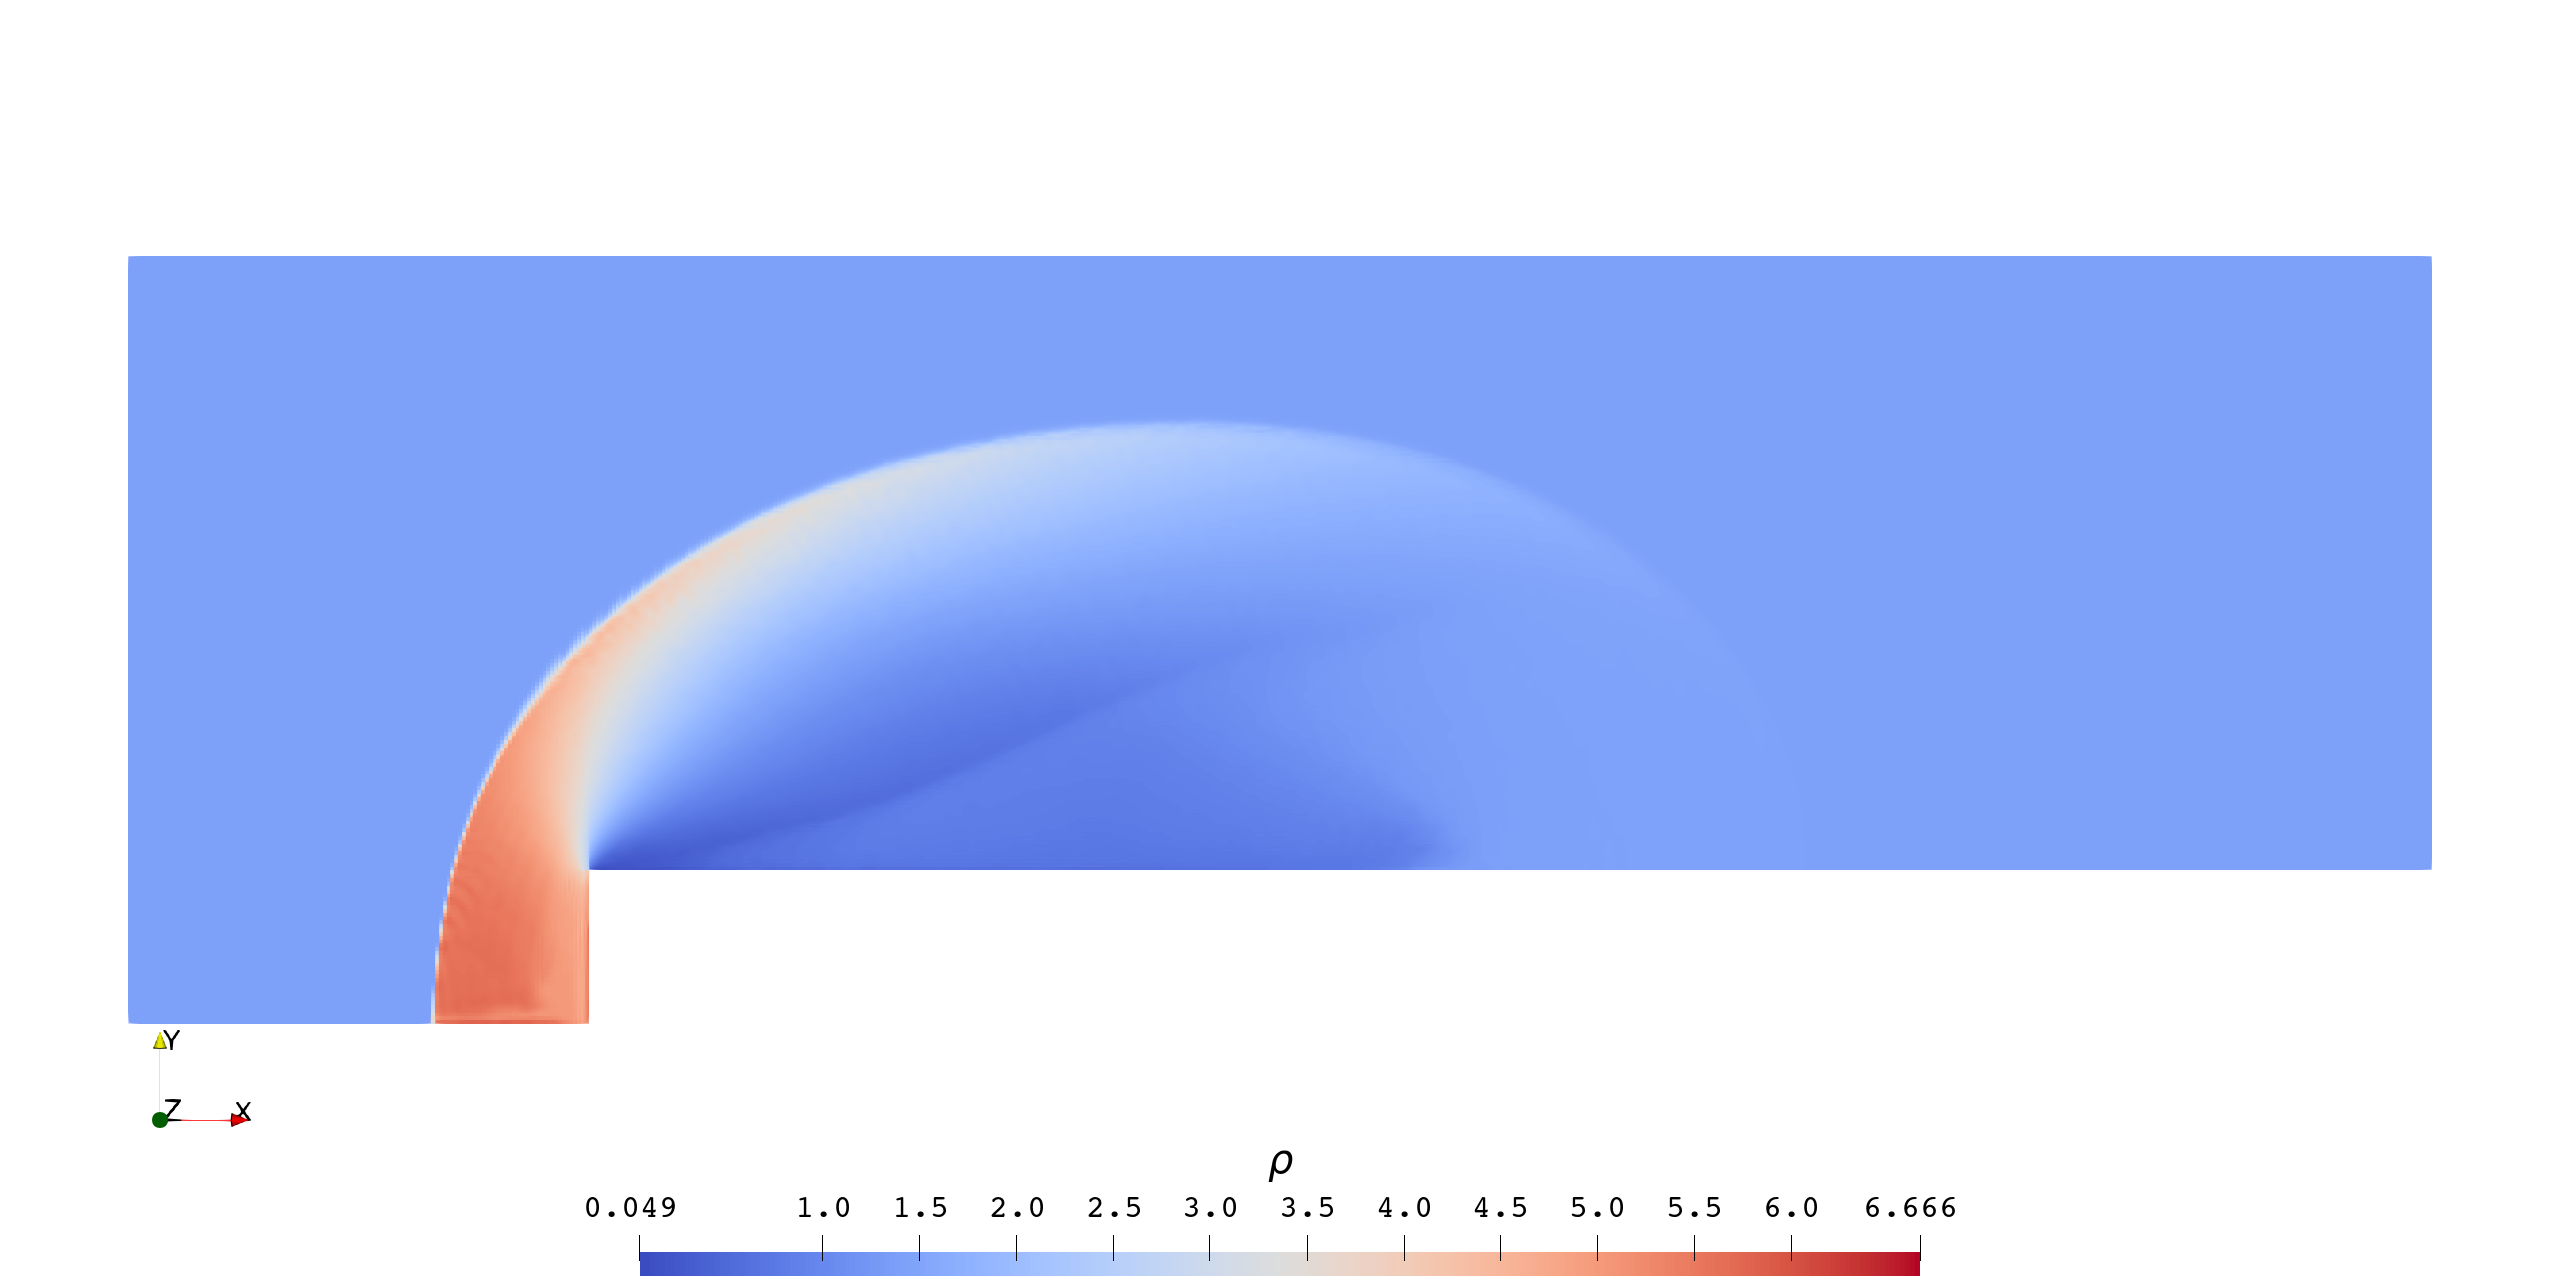
\includegraphics[width=1\textwidth,height=0.28\textheight]{../mdpi/figures/forward_step/p=3_t=04e-1}
\par\end{centering}
\caption{\label{fig:forward_step_p=00003D3_t=00003D04e-1}在 $h=1/200$ 的伪结构网格上所得\nameref{prob:=00524D=005411=0053F0=009636}问题在
$t=0.4$ 时刻的 RK3/DG3 近似解}
\end{figure}

大约在 $t=0.6$ 时刻,该弓形激波与风洞顶部发生碰撞并发生反射,如图 \ref{fig:forward_step_p=00003D3_t=00003D06e-1}
所示。该反射为常规反射,反射波向风洞底部运动,如图 \ref{fig:forward_step_p=00003D3_t=00003D08e-1}、图
\ref{fig:forward_step_p=00003D3_t=00003D10e-1} 所示。

\begin{figure}[h!]
\begin{centering}
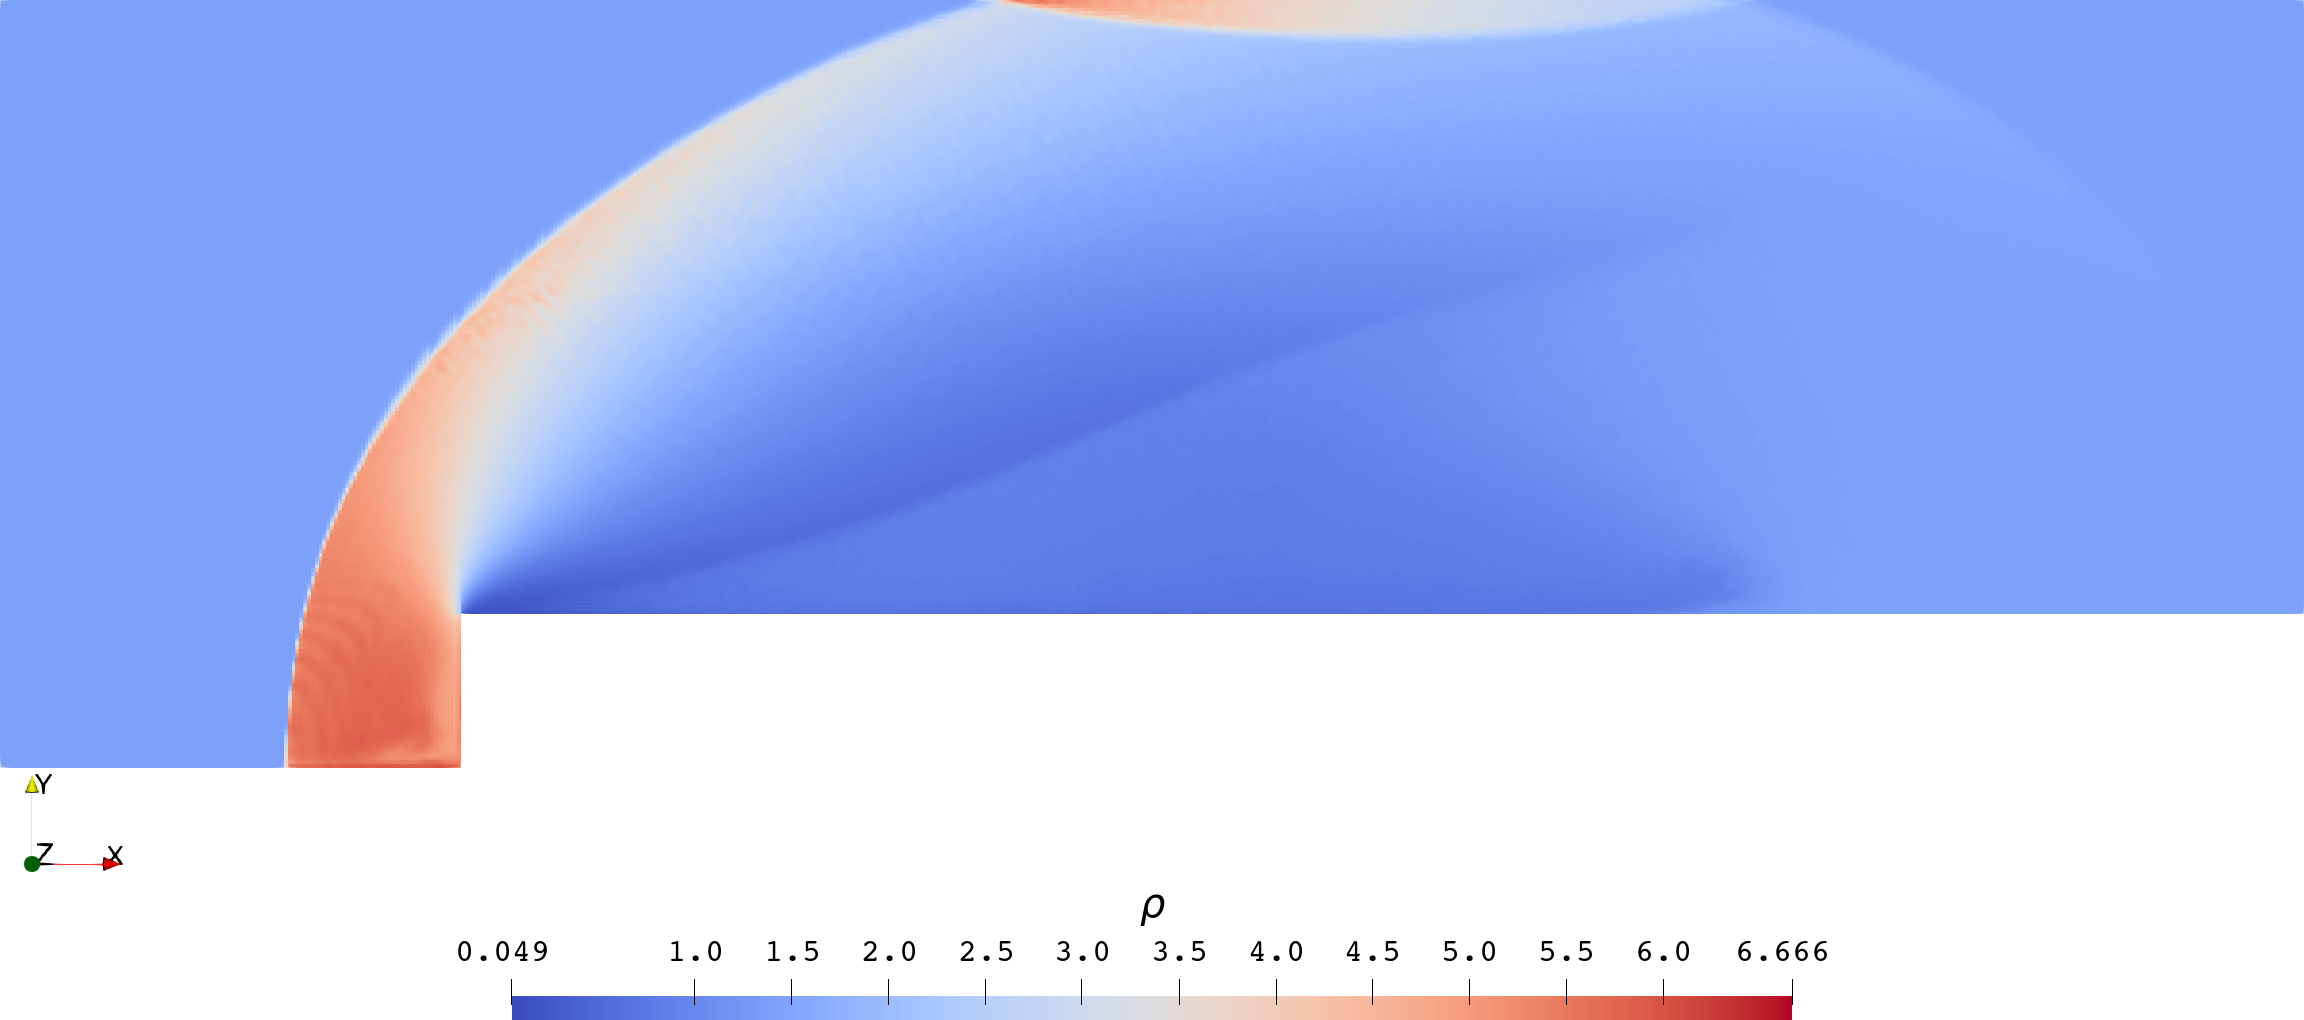
\includegraphics[width=1\textwidth,height=0.28\textheight]{../mdpi/figures/forward_step/p=3_t=06e-1}
\par\end{centering}
\caption{\label{fig:forward_step_p=00003D3_t=00003D06e-1}在 $h=1/200$ 的伪结构网格上所得\nameref{prob:=00524D=005411=0053F0=009636}问题在
$t=0.6$ 时刻的 RK3/DG3 近似解}
\end{figure}

\begin{figure}[h!]
\begin{centering}
\includegraphics[width=1\textwidth,height=0.28\textheight]{../mdpi/figures/forward_step/p=3_t=08e-1}
\par\end{centering}
\caption{\label{fig:forward_step_p=00003D3_t=00003D08e-1}在 $h=1/200$ 的伪结构网格上所得问题
\nameref{prob:=00524D=005411=0053F0=009636} 在 $t=0.8$ 时刻的 RK3/DG3
近似解}
\end{figure}

\begin{figure}[h!]
\begin{centering}
\includegraphics[width=1\textwidth,height=0.28\textheight]{../mdpi/figures/forward_step/p=3_t=10e-1}
\par\end{centering}
\caption{\label{fig:forward_step_p=00003D3_t=00003D10e-1}在 $h=1/200$ 的伪结构网格上所得\nameref{prob:=00524D=005411=0053F0=009636}问题在
$t=1.0$ 时刻的 RK3/DG3 近似解}
\end{figure}

大约在 $t=1.2$ 时刻,反射波与台阶顶部发生碰撞并再次反射,如图 \ref{fig:forward_step_p=00003D3_t=00003D12e-1}
所示。

\begin{figure}[h!]
\begin{centering}
\includegraphics[width=1\textwidth,height=0.28\textheight]{../mdpi/figures/forward_step/p=3_t=12e-1}
\par\end{centering}
\caption{\label{fig:forward_step_p=00003D3_t=00003D12e-1}在 $h=1/200$ 的伪结构网格上所得\nameref{prob:=00524D=005411=0053F0=009636}问题在
$t=1.2$ 时刻的 RK3/DG3 近似解}
\end{figure}

大约在 $t=2.0$ 时刻,该二级反射依然为常规反射,但风洞顶部的初级反射已发展为马赫反射,如图 \ref{fig:forward_step_p=00003D3_t=00003D20e-1}
所示。垂直于壁面的马赫杆,入射波、反射波、马赫杆汇聚处的三岔点,以及自三岔点向后拖出的剪切层,正是马赫反射的标志性特征。

\begin{figure}[h!]
\begin{centering}
\includegraphics[width=1\textwidth,height=0.28\textheight]{../mdpi/figures/forward_step/p=3_t=20e-1}
\par\end{centering}
\caption{\label{fig:forward_step_p=00003D3_t=00003D20e-1}在 $h=1/200$ 的伪结构网格上所得\nameref{prob:=00524D=005411=0053F0=009636}问题在
$t=2.0$ 时刻的 RK3/DG3 近似解}
\end{figure}

此后一段时间,马赫杆逐渐拉长,二级反射波逐渐靠近风洞顶部,如图 \ref{fig:forward_step_p=00003D3_t=00003D24e-1}
所示。

\begin{figure}[h!]
\begin{centering}
\includegraphics[width=1\textwidth,height=0.28\textheight]{../mdpi/figures/forward_step/p=3_t=24e-1}
\par\end{centering}
\caption{\label{fig:forward_step_p=00003D3_t=00003D24e-1}在 $h=1/200$ 的伪结构网格上所得\nameref{prob:=00524D=005411=0053F0=009636}问题在
$t=2.4$ 时刻的 RK3/DG3 近似解}
\end{figure}

大约在 $t=2.8$ 时刻,二级反射波与风洞顶部发生碰撞并形成三级反射,如图 \ref{fig:forward_step_p=00003D3_t=00003D28e-1}
所示。不难想象,如果风洞的长度足够长,且计算的时间范围也足够大,那么这种反射的级数还有可能继续增加。

\begin{figure}[h!]
\begin{centering}
\includegraphics[width=1\textwidth,height=0.28\textheight]{../mdpi/figures/forward_step/p=3_t=28e-1}
\par\end{centering}
\caption{\label{fig:forward_step_p=00003D3_t=00003D28e-1}在 $h=1/200$ 的伪结构网格上所得\nameref{prob:=00524D=005411=0053F0=009636}问题在
$t=2.8$ 时刻的 RK3/DG3 近似解}
\end{figure}

自 $t=2.8$ 时刻起,到 $t=4.0$ 时刻止,一个显著发展的流动特征是三叉点后的波纹状剪切层涡系,如图 \ref{fig:forward_step_p=00003D3_t=00003D28e-1}–\ref{fig:forward_step_p=00003D3_t=00003D40e-1}
所示。文献 \cite{Woodward_1984} 认为,这种波纹的形成是数值误差引起的扰动被剪切层的开尔文–亥姆霍兹不稳定性捕获的结果。虽然该涡系的形成有非物理的原因,但对其细节的分辨能力已经成为了评价求解器性能的一个定性指标,更低阶的求解器或更粗糙的网格都很难捕获该流动特征。

\begin{figure}[h!]
\begin{centering}
\includegraphics[width=1\textwidth,height=0.28\textheight]{../mdpi/figures/forward_step/p=3_t=32e-1}
\par\end{centering}
\caption{\label{fig:forward_step_p=00003D3_t=00003D32e-1}在 $h=1/200$ 的伪结构网格上所得\nameref{prob:=00524D=005411=0053F0=009636}问题在
$t=3.2$ 时刻的 RK3/DG3 近似解}
\end{figure}

\begin{figure}[h!]
\begin{centering}
\includegraphics[width=1\textwidth,height=0.28\textheight]{../mdpi/figures/forward_step/p=3_t=40e-1}
\par\end{centering}
\caption{\label{fig:forward_step_p=00003D3_t=00003D40e-1}在 $h=1/200$ 的伪结构网格上所得\nameref{prob:=00524D=005411=0053F0=009636}问题在
$t=4.0$ 时刻的 RK3/DG3 近似解}
\end{figure}

\begin{figure}[h!]
\begin{centering}
\includegraphics[width=1\textwidth,height=0.28\textheight]{../mdpi/figures/forward_step/p=3_t=40e-1}
\par\end{centering}
\caption{\label{fig:forward_step_p=00003D3_t=00003D40e-1-1}在 $h=1/200$ 的伪结构网格上所得\nameref{prob:=00524D=005411=0053F0=009636}问题在
$t=4.0$ 时刻的 RK3/DG3 近似解}
\end{figure}

为了定性验证以上结果的正确性,图 \ref{fig:forward_step_p=00003D5_qiu} 给出了文献 \cite{Giri_2019}
在三级自适应加密(最粗处 $h\approx1/32$,最细处 $h\approx1/256$)的三角形网格上所得二维 RK3/DG5
近似解,它是该问题目前已发表的最高精度的近似解。将其与图 \ref{fig:double_mach_p=00003D3_h=00003D5e-3}
即本文在 $h=1/200$ 的伪结构网格上所得三维 RK3/DG3 近似解对比,不难发现:二者给出的流场结构非常相似,这说明本文所实现的三维
RK3/DG3 求解器能够在三维伪结构网格上正确地捕捉复杂的二维流场结构。

\begin{figure}[h!]
\begin{centering}
\includegraphics[width=1\textwidth]{figures/forward_step/qiu}
\par\end{centering}
\caption{\label{fig:forward_step_p=00003D5_qiu}在三级自适应加密的二维非结构网格上所得\nameref{prob:=00524D=005411=0053F0=009636}问题
$\rho(x,y,t=4)$ 的 RK3/DG5 近似解\upcite{Giri_2019}}
\end{figure}


\section{本章小结}

本章基于大量算例,对第\ref{chap:=007B97=006CD5}章所提高阶计算格式的精度做了充分的验证。计算结果表明,带有
WENO 限制器的高阶 RKDG 格式具有以下优点:
\begin{description}[wide]
\item [{基本无振荡}] 该格式能够将高阶近似解在(解析解、数值精确解所给出的)间断附近的数值振荡,压制到几乎无法察觉的程度,避免了密度或压强出现负值。激波在近似解中的厚度大约为
$1h$ 到 $3h$,接触间断在近似解中的厚度大约为 $5h$ 到 $7h$,均远小于经典有限体积近似解的相应厚度。
\item [{数值耗散低}] 该格式能够在相对较粗的非结构网格上捕获复杂的流动细节——特别是那些容易被数值耗散磨平的涡结构。这一点对于模拟由桨尖涡主导的旋翼尾迹是十分有利的。除此之外,下一章将会看到:高阶
UMS–RKDG 近似解还能在相对较粗的非结构网格上捕捉到声波。
\item [{计算效率高}] 尽管高阶格式在每个单元上的计算量大于低阶格式,但高阶格式所特有的低数值耗散的优势,使得其在粗网格上近似解,具有与细网格上的低阶近似解接近的精度。对运行时间和存储空间的测量(如表
\ref{tab:linear_cost}、表 \ref{tab:sod_cost} 所示)表明:高阶 RKDG 近似解具有更高的计算效率,即在全局精度接近的前提下,粗网格上的高阶近似解比细网格上的低阶近似解更省时间(用电量)。
\end{description}


\chapter{旋翼流场计算的并行加速及性能测评\label{chap:=005E76=00884C}}

如第\ref{chap:=007B97=006CD5}章所述,本文所提出的旋翼流场计算方法,是将模拟旋翼气动力的 UMS 模型植入带有紧致
WENO 限制器的 RKDG 格式而得到的。后者自从被提出以来,鲜有三维工程应用的报道。一个重要原因是每个单元所消耗的计算资源,随着精度阶数或空间维度的增加而迅速增长。另一方面,显式
RKDG 格式和紧致 WENO 限制器的大多数计算都可以在本地进行,并且不需要求解全局代数方程组。因此,基于区域分解的分布式并行计算可以很自然地被用来加速计算。目前(2022
年初),带有紧致 WENO 限制器的 RKDG 格式还没有公开发表的并行实现。其他的 DG 格式虽有公开发表的并行实现,例如:
\begin{itemize}
\item Biswas 等\upcite{Biswas_1994} 在均匀结构网格上,测量了其一维、二维线性标量问题 DG 求解器的并行性能。他们获得了接近理想情形的并行效率:纯求解时间(无
I/O)超过 99\%,总运行时间至少 89\%。
\item Bey 等\upcite{Bey_1995} 在均匀(结构)和 $hp$-自适应(非结构)网格上,测试了其线性守恒律 DG 求解器的性能。当内部单元的数量远超边界单元的数量时,他们获得了几乎最优的并行效率。
\item Chalmers 等\upcite{Chalmers_2019}使用 MPI/OpenMP 混合并行,实现了二维 Navier–Stokes
方程 DG 格式的并行化,并在只有四边形单元的均匀网格上实现了良好的可扩展性。
\end{itemize}
但都没有给出其在三维非结构网格上的并行性能。

为了让第\ref{chap:=007B97=006CD5}章所述、第\ref{chap:=009A8C=008BC1}章所验证的高阶计算格式具有实用价值,本章将提出并实现一种分布式并行加速方案,并在实验室自建的
100 核“机群 (cluster)”上测量加速比及并行效率,以评估该方案的性能。

\section{旋翼流场计算\label{sec:rotor_in_tunnel}}

本节用图 \ref{fig:rotor_mesh} 所示的网格,模拟孤立旋翼在低速风洞中的吹风试验。风洞外形由三维区间 $[\SI{-3}{m},\SI{9}{m}]\times[\SI{-3}{m},\SI{3}{m}]\times[\SI{-3}{m},\SI{3}{m}]$
表示,在其内部嵌套一个较小的三维区间 $[\SI{-2}{m},\SI{8}{m}]\times[\SI{-2}{m},\SI{2}{m}]\times[\SI{-2}{m},\SI{2}{m}]$,用以表示旋翼及其尾迹附近网格需要加密的区域。旋翼桨盘中心固定于坐标原点处,桨根及桨尖到该中心点的距离分别为
$\SI{0.1}{m}$ 与 $\SI{1.0}{m}$,因此桨盘直径为 $\SI{2.0}{m}$。旋翼转轴允许指向任意方向,转速为每秒
$40$ 转,桨尖速率约为 $0.74$ 马赫(声速取 $\SI{340}{m/s}$)。图 \ref{fig:rotor_mesh}
中的球形区域(即半径为 $\SI{1.0}{m}$ 的球体)表示桨叶可能扫过的区域,原则上可以在该区域内进一步加密网格。

\begin{figure}[h!]
\begin{centering}
\includegraphics[width=1\textwidth,height=0.33\textheight,keepaspectratio]{../mdpi/figures/rotor_in_tunnel/mesh}
\par\end{centering}
\caption{\label{fig:rotor_mesh}\nameref{prob:=005B64=007ACB=0065CB=007FFC=008F74=005411=008FCE=0098CE}、\nameref{prob:=005B64=007ACB=0065CB=007FFC=005F84=005411=008FCE=0098CE}问题所用网格的示意图}
\end{figure}

桨叶选用单一翼型、弦长为 $\SI{0.1}{m}$ 的矩形平直桨叶,预扭角为 $\ang{10}$;翼型选用 UH-60A 直升机主旋翼的
SC-1095 翼型,其升力系数、阻力系数曲线分别如图 \ref{fig:rotor_c_lift}、图 \ref{fig:rotor_c_drag}
所示,用于作图的数据引自文献 \cite{Howlett_1981}。对于更一般的翼型,可以通过吹风试验或数值模拟来获得类似的曲线。

\begin{figure}[h!]
\begin{centering}
\includegraphics[width=1\textwidth,height=0.26\textheight,keepaspectratio]{figures/airfoil/lift}
\par\end{centering}
\caption{\label{fig:rotor_c_lift}SC-1095 翼型的升力系数曲线\upcite{Howlett_1981}}
\end{figure}

\begin{figure}[h!]
\begin{centering}
\includegraphics[width=1\textwidth,height=0.26\textheight,keepaspectratio]{figures/airfoil/drag}
\par\end{centering}
\caption{\label{fig:rotor_c_drag}SC-1095 翼型的阻力系数曲线\upcite{Howlett_1981}}
\end{figure}

以上几何参数以及本节剩余部分给出的定解条件,是对真实旋翼风洞试验的较为激进的简化。进行这种简化主要是为了方便后续计算或试验研究复现本节剩余部分给出的算例。实际上,对于更一般的风洞截面形状,获得如图
\ref{fig:rotor_mesh} 所示的只含四面体单元的非结构网格,对于网格生成模块而言没有额外的难度;对于更一般的桨叶外形,如非线性的弦长、预扭分布,本文所实现的求解器也已支持对其进行高效处理。

\subsection{孤立旋翼轴向迎风}

该问题是对直升机爬升工况的简化。
\begin{problem}
[孤立旋翼轴向迎风]\label{prob:=005B64=007ACB=0065CB=007FFC=008F74=005411=008FCE=0098CE}令旋翼转轴指向风洞左侧,即以
$(-1,0,0)$ 为方向矢量。

在时间范围 $t\in[0,1]$ 内,求满足三维欧拉方程 (\ref{eq:euler_system}) 及以下定解条件的广义解。

初始条件设为均匀低速气流:
\begin{equation}
\begin{bmatrix}\rho & u_{x} & u_{y} & u_{z} & p\end{bmatrix}_{t=0}=\begin{bmatrix}1.29 & 1.0 & 0.0 & 0.0 & 101325.0\end{bmatrix}.
\end{equation}

边界条件如下:
\begin{itemize}
\item 风洞左端为亚声速入口,状态与初始条件兼容:
\begin{equation}
\begin{bmatrix}\rho & u_{x} & u_{y} & u_{z} & p\end{bmatrix}_{x=-3}=\begin{bmatrix}\rho & u_{x} & u_{y} & u_{z} & p\end{bmatrix}_{t=0};
\end{equation}
\item 风洞右端为亚声速出口,只给定背景压强:
\begin{equation}
\eval{p}_{x=9}=101325.0;
\end{equation}
\item 风洞上、下、前、后四面均为固体壁面。\qedhere
\end{itemize}
\end{problem}

为了体现高阶求解器在粗网格上的优势,这里采用只含 $h\approx0.25$ 的四面体单元的粗网格求解该问题。图 \ref{fig:upward_p=00003D1}
与图 \ref{fig:upward_p=00003D3} 分别给出了\nameref{prob:=005B64=007ACB=0065CB=007FFC=008F74=005411=008FCE=0098CE}问题在若干时刻的
UMS–RK1/DG1 与 UMS–RK3/DG3 近似解。这里给出精度较低的 UMS–RK1/DG1 近似解,是因为其在物理上较为可靠,可以用来定性地验证高阶近似解的正确性。

\begin{figure}[h!]
\begin{centering}
\subfloat[\label{fig:upward_t=00003D4e-1_p=00003D1}$t=0.4$]{\begin{centering}
\includegraphics[width=1\textwidth,height=0.4\textheight,keepaspectratio]{figures/upward/p=1/Frame40}
\par\end{centering}
}
\par\end{centering}
\begin{centering}
\subfloat[\label{fig:upward_t=00003D8e-1_p=00003D1}$t=0.8$]{\begin{centering}
\includegraphics[width=1\textwidth,height=0.4\textheight,keepaspectratio]{figures/upward/p=1/Frame80}
\par\end{centering}
}
\par\end{centering}
\caption{\label{fig:upward_p=00003D1}\nameref{prob:=005B64=007ACB=0065CB=007FFC=008F74=005411=008FCE=0098CE}问题的
UMS–RK1/DG1 近似解}
\end{figure}

图 \ref{fig:upward_p=00003D1} 与图 \ref{fig:upward_p=00003D3} 采取了相同的作图方式:在
$y=0$ 平面上画出密度分布;在 $z=0$ 平面上画出速度方向,并以箭头根部密度着色;偏左侧的一对同心圆表示桨尖及桨根轨迹。

不难发现:桨盘上(左)侧的速度矢量明显在向中心汇聚,密度值在桨盘附近有一个明显的跳跃。由等熵条件 $p=C\rho^{\gamma}$
可以推知,压强在桨盘附近也有一跳跃,且下(右)侧值大于上(左)侧值。这说明流经桨盘平面的气体,正在被桨叶压缩做功;根据牛顿第三定律,桨叶必然受到气体对其施加的反作用力,这正是旋翼升力的来源。

\begin{figure}[h!]
\begin{centering}
\subfloat[\label{fig:upward_t=00003D4e-1_p=00003D3}$t=0.4$]{\begin{centering}
\includegraphics[width=1\textwidth,height=0.4\textheight,keepaspectratio]{figures/upward/p=3/Frame40}
\par\end{centering}
}
\par\end{centering}
\begin{centering}
\subfloat[\label{fig:upward_t=00003D8e-1_p=00003D3}$t=0.8$]{\begin{centering}
\includegraphics[width=1\textwidth,height=0.4\textheight,keepaspectratio]{figures/upward/p=3/Frame80}
\par\end{centering}
}
\par\end{centering}
\caption{\label{fig:upward_p=00003D3}\nameref{prob:=005B64=007ACB=0065CB=007FFC=008F74=005411=008FCE=0098CE}问题的
UMS–RK3/DG3 近似解}
\end{figure}

比较不同时刻的 UMS–RK1/DG1、UMS–RK3/DG3 近似解可以发现:两种求解器都能捕捉大尺度的涡结构,例如形成于桨盘下(右)侧、随时间推移而向下(右)移动的环状涡;但只有
UMS–RK3/DG3 求解器才能在如此稀疏的网格上捕捉到声波的干涉条纹。这是因为 UMS–RK1/DG1 求解器采用分段常值近似,过大的数值耗散容易将流动细节抹平。

数值耗散的强弱,还可以通过环状涡的涡核清晰度来观察。图 \ref{fig:upward_ring} 补充显示了 $x=4.8$
平面上的密度分布。可以发现:环状涡的涡核在 UMS–RK1/DG1 近似解中较为模糊,在 UMS–RK3/DG3 近似解中仍十分明显。这再次体现了高阶求解器数值耗散低的优势。

\begin{figure}[h!]
\begin{centering}
\subfloat[\label{fig:upward_ring_p=00003D1}$p=1$(时空一阶)]{\begin{centering}
\includegraphics[width=1\textwidth,height=0.4\textheight,keepaspectratio]{figures/upward/p=1/vortex}
\par\end{centering}
}
\par\end{centering}
\begin{centering}
\subfloat[\label{fig:upward_ring_p=00003D3}$p=3$(时空三阶)]{\begin{centering}
\includegraphics[width=1\textwidth,height=0.4\textheight,keepaspectratio]{figures/upward/p=3/vortex}
\par\end{centering}
}
\par\end{centering}
\caption{\label{fig:upward_ring}\nameref{prob:=005B64=007ACB=0065CB=007FFC=008F74=005411=008FCE=0098CE}问题在
$t=1.0$ 时刻的 UMS–RKDG 近似解(补充显示起动涡)}
\end{figure}

\newpage{}

\subsection{孤立旋翼径向迎风}

该问题是对直升机前飞工况的简化。
\begin{problem}
[孤立旋翼径向迎风]\label{prob:=005B64=007ACB=0065CB=007FFC=005F84=005411=008FCE=0098CE}令旋翼转轴指向风洞顶部,即以
$(0,0,1)$ 为方向矢量。

在时间范围 $t\in[0,1]$ 内,求满足三维欧拉方程 (\ref{eq:euler_system}) 及以下定解条件的广义解。

初始条件设为均匀中低速气流:
\begin{equation}
\begin{bmatrix}\rho & u_{x} & u_{y} & u_{z} & p\end{bmatrix}_{t=0}=\begin{bmatrix}1.29 & 10.0 & 0.0 & 0.0 & 101325.0\end{bmatrix}.
\end{equation}

边界条件在形式上与\nameref{prob:=005B64=007ACB=0065CB=007FFC=008F74=005411=008FCE=0098CE}问题相同。
\end{problem}

为体现高阶解的优势,这里仍采用 $h\approx0.25$ 的粗网格求解该问题。图 \ref{fig:forward_p=00003D1}
与图 \ref{fig:forward_p=00003D3} 分别给出了该问题在若干时刻的 UMS–RK1/DG1、UMS–RK3/DG3
近似解。

\begin{figure}[h!]
\begin{centering}
\subfloat[\label{fig:forward_t=00003D4e-1_p=00003D1}$t=0.4$]{\begin{centering}
\includegraphics[width=1\textwidth,height=0.4\textheight,keepaspectratio]{figures/forward/p=1/Frame40}
\par\end{centering}
}
\par\end{centering}
\begin{centering}
\subfloat[\label{fig:forward_t=00003D10e-1_p=00003D1}$t=1.0$]{\begin{centering}
\includegraphics[width=1\textwidth,height=0.4\textheight,keepaspectratio]{figures/forward/p=1/Frame100}
\par\end{centering}
}
\par\end{centering}
\caption{\label{fig:forward_p=00003D1}\nameref{prob:=005B64=007ACB=0065CB=007FFC=005F84=005411=008FCE=0098CE}问题的
UMS–RK1/DG1 近似解}
\end{figure}

\newpage{}

图 \ref{fig:forward_p=00003D1} 与图 \ref{fig:forward_p=00003D3} 的作图方式为:在
$x=4$ 平面上画出密度分布;在 $y=0$ 平面上画出速度方向,并以箭头根部密度着色;偏左侧的一对同心圆表示桨尖及桨根轨迹。

不难发现:桨盘附近的速度矢量明显向下偏转,这表明旋转的桨叶在为气流提供动量;旋翼尾迹(红色区域)向右偏转,这体现了左侧自由来流的驱动作用。

\begin{figure}[h!]
\begin{centering}
\subfloat[\label{fig:forward_t=00003D4e-1_p=00003D3}$t=0.4$]{\begin{centering}
\includegraphics[width=1\textwidth,height=0.4\textheight,keepaspectratio]{figures/forward/p=3/Frame40}
\par\end{centering}
}
\par\end{centering}
\begin{centering}
\subfloat[\label{fig:forward_t=00003D10e-1_p=00003D3}$t=1.0$]{\begin{centering}
\includegraphics[width=1\textwidth,height=0.4\textheight,keepaspectratio]{figures/forward/p=3/Frame100}
\par\end{centering}
}
\par\end{centering}
\caption{\label{fig:forward_p=00003D3}\nameref{prob:=005B64=007ACB=0065CB=007FFC=005F84=005411=008FCE=0098CE}问题的
UMS–RK3/DG3 近似解}
\end{figure}

与\nameref{prob:=005B64=007ACB=0065CB=007FFC=008F74=005411=008FCE=0098CE}问题的结论类似,两种求解器都能捕捉大尺度的涡结构,例如从桨盘拖出、向右下方倾斜的旋翼尾迹;但只有
UMS–RK3/DG3 求解器才能在 $x=4$ 平面上捕捉到一对清晰的涡核(深蓝色区域)。下面采用两种方法来显示这对涡。

\newpage{}

第一种方法基于速度流线,它是对瞬时速度场的空间积分:
\begin{equation}
\vec{r}(s)\coloneqq\vec{r}_{0}+\int_{s_{0}}^{s}\vec{u}\dd{\sigma}.
\end{equation}

图 \ref{fig:forward_streamlines} 画出了由 $t=1.0$ 时刻的 UMS–RK3/DG3 近似解导出的速度流线。可以看出:桨盘两侧的流线在向后延伸的过程中,叠加了绕某个向后延伸的轴线的转动,该轴线恰好穿过图
\ref{fig:forward_t=00003D10e-1_p=00003D3} 中的低密度区(即涡核所在位置)。这说明,由 UMS–RK3/DG3
近似解导出的结果是自洽的。

\begin{figure}[h!]
\begin{centering}
\subfloat[主视图]{\begin{centering}
\includegraphics[width=1\textwidth,height=0.4\textheight,keepaspectratio]{figures/forward/p=3/y+}
\par\end{centering}
}
\par\end{centering}
\begin{centering}
\subfloat[俯视图]{\begin{centering}
\includegraphics[width=1\textwidth,height=0.4\textheight,keepaspectratio]{figures/forward/p=3/z-}
\par\end{centering}
}
\par\end{centering}
\caption{\label{fig:forward_streamlines}由\nameref{prob:=005B64=007ACB=0065CB=007FFC=005F84=005411=008FCE=0098CE}问题在
$t=1.0$ 时刻的 UMS–RK3/DG3 近似解导出的速度流线图}
\end{figure}

\newpage{}

第二种方法基于 $Q$ 值\upcite{Jeong_1995},它是速度梯度张量的第二不变量:
\begin{equation}
Q\coloneqq\frac{(\partial_{i}u_{i})(\partial_{k}u_{k})-(\partial_{i}u_{k})(\partial_{k}u_{i})}{2}
\end{equation}

图 \ref{fig:forward_Q} 画出了由 $t=1.0$ 时刻的 UMS–RK1/DG1 近似解导出的 $Q$ 等值面。可以看出:桨盘两侧各有一道向后拖出的涡,且其位置与图
\ref{fig:forward_streamlines} 中流线螺旋延伸的轴线一致。这说明由两种近似解导出的结果是相容的。

\begin{figure}[h!]
\begin{centering}
\subfloat[主视图]{\begin{centering}
\includegraphics[width=1\textwidth,height=0.4\textheight,keepaspectratio]{figures/forward/p=1/Q_y+}
\par\end{centering}
}
\par\end{centering}
\begin{centering}
\subfloat[俯视图]{\begin{centering}
\includegraphics[width=1\textwidth,height=0.4\textheight,keepaspectratio]{figures/forward/p=1/Q_z-}
\par\end{centering}
}
\par\end{centering}
\caption{\label{fig:forward_Q}由\nameref{prob:=005B64=007ACB=0065CB=007FFC=005F84=005411=008FCE=0098CE}问题在
$t=1.0$ 时刻的 UMS–RK1/DG1 近似解导出的 $Q$ 等值面}
\end{figure}

\newpage{}

\section{并行加速方案\label{sec:parallel}}

\nomenclature{CPU}{central processing unit}


\subsection{非结构网格分块}

CFD 所用的“网格 (mesh)”是一种特殊的“图 (graph)”数据结构\upcite{Sedgewick_2011}。前者可以通过调用
METIS\upcite{Karypis_1998} 提供的 \texttt{METIS\_PartMeshDual(...)} 来实现分块,后者的分块可以通过调用
\texttt{METIS\_PartGraphKway(...)} 或 \texttt{METIS\_PartGraphRecursive(...)}
来完成。实际上,网格分块函数 \texttt{METIS\_PartMeshDual(...)} 的内部封装了对图分块函数的调用,只不过这里被分块的是网格的“对偶图
(dual graph)”。所谓网格的对偶图,是指以体单元为顶点、以体单元邻接关系为边的图。METIS 提供了 \texttt{METIS\_MeshToDual(...)},用于将非结构网格转化为其对偶图。

RKDG 格式中的面积分残差,即式 (\ref{eq:boundary_residual}),以及 WENO 重构过程中遍历邻接单元的操作,都对体单元访问其邻接单元的效率提出了很高的要求:各体单元应能在常数时间内访问其任意邻接单元。就非结构网格而言,这意味着每个体单元都要预先存储其所有邻接单元的指针(或引用)。单元的邻接关系隐含在结点的连接关系里,因此大多数网格文件格式都不会显式记录该信息。

出于上述原因,本文不像传统的并行有限元方法那样直接对网格分块,而是先用 \texttt{METIS\_MeshToDual(...)}
将非结构网格转化为其对偶图,再用 \texttt{METIS\_PartGraphKway(...)} 或 \texttt{METIS\_PartGraphRecursive(...)}
对该对偶图实施分块。需要注意的是,用 C 语言编写的 \texttt{METIS\_MeshToDual(...)} 函数,将单元邻接信息存储在动态分配的数组里,并返回指向该数组头部的地址。为避免内存泄漏造成动态内存空间耗尽,该动态数组必须被调用栈里的某一个且只有一个调用者释放。利用现代
C++ 标准库提供的智能指针接管该动态数组,能够有效地避免动态内存忘记释放或释放不止一次等内存故障\upcite{Meyers_2014}。

\subsection{进程间消息传递}

获得网格分块后,每一块上的数据都应由一个进程加载。各进程串行地保存和更新本地数据,并在必要时与邻居交换公共边界上的数据。这是分布式并行计算的典型场景,它通过在多个处理器核心上同时解决规模相等或接近的子问题来实现加速。与之相比,由多个线程共享同一内存空间的并行程序通常更易于编写,但存在扩展性瓶颈,通常只适用于安装有多核处理器的单机并行计算。

为保持扩展性,本文选择分布式并行方案。为此,需要付出的代价是显式传递消息,以实现进程之间的数据交互。得益于学术界和工业界的共同努力,MPI
已经成为事实上的分布式并行计算行业标准,被称为“并行计算的汇编语言”。

为了提高代码的可读性和可维护性,本文将涉及通信的操作封装在名为 \texttt{ShareSomething(...)} 的一组函数中,它们拥有相同的代码结构:
\begin{enumerate}[wide]
\item 为每个目的地,将要发送的数据放入发送缓冲区,并通过调用 \texttt{MPI\_Isend(...)} 函数注册发送请求。
\item 为每个源进程,分配一个接收缓冲区用于接收数据,并通过调用 \texttt{MPI\_Irecv(...)} 函数注册一个接收请求。
\item 执行无需通信即可完成的其他计算任务。
\item 通过调用 \texttt{MPI\_Waitall(...)} 函数阻塞所有进程,直到其所有发送和接收请求完成。
\end{enumerate}

以上各步中,第 3 步是可选的,它允许计算与通信重叠,有助于提高并行效率;第 4 步是显式同步操作,除此之外还有一些隐式同步(例如:向同一个文件并行地写入数据),它们是降低并行性能的直接因素,应尽量避免非必要的同步。

\section{并行性能测评}

\subsection{双马赫反射问题}

本小节对第\ref{chap:=009A8C=008BC1}章用于验证近似解精度的\nameref{prob:=0053CC=009A6C=008D6B=0053CD=005C04}问题做并行性能测评。该问题的初边值条件及近似解具有二维特征,因此在三维空间求解时,沿
$z$ 方向的网格数量可以很少(本文尝试过取一到三层,所得结果没有显著变化)。因此,对这种伪三维网格的分块,实际上等价于对二维网格的分块。这就造成各块边界上的单元数量,近似为块内单元数量的
$\order{N^{1/2}}$;而对真正的三维网格分块,各块边界上的单元数量,近似为块内单元数量的 $\order{N^{2/3}}$。由此可以预测:本节所得并行效率将高于真正三维问题的并行效率。这一预测将被本章
\ref{subsec:rotor-parallel} 小节的数据所证实。

虽然在求解\nameref{prob:=0053CC=009A6C=008D6B=0053CD=005C04}问题时使用了非结构网格,但其所含单元的尺寸大致相等,且计算区域具有简单的几何外形,因此很容易得到较为均匀的网格分块,从而实现静态负载均衡。为了提高求解器的普适性,我们放弃了这种简单几何外形带来的便利,转而通过调用第三方库
METIS\upcite{Karypis_1998} 来实施网格分块。图 \ref{fig:double_mach_partition}、图
\ref{fig:double_mach_balance} 给出了将图 \ref{fig:double_mach_p=00003D1_h=00003D5e-3}–\ref{fig:double_mach_p=00003D3_h=00003D5e-3}
中的非结构网格分割为 100 块的(某次)分块结果,可见单元数量的波动小于 $3\%$,大致呈均匀分布。考虑到非结构网格的均匀分块属于
NP-hard 问题,图 \ref{fig:double_mach_partition}、图 \ref{fig:double_mach_balance}
所示的分块效果已经相当令人满意。

\begin{figure}[h!]
\begin{centering}
\includegraphics[width=1\textwidth,height=0.4\textheight,keepaspectratio]{figures/double_mach/partition}
\par\end{centering}
\caption{\label{fig:double_mach_partition}将\nameref{prob:=0053CC=009A6C=008D6B=0053CD=005C04}问题所用非结构网格分割为
$100$ 块的分块结果}
\end{figure}

\begin{figure}[h!]
\begin{centering}
\includegraphics[width=1\textwidth,height=0.3\textheight,keepaspectratio]{figures/double_mach/balance}
\par\end{centering}
\caption{\label{fig:double_mach_balance}\nameref{prob:=0053CC=009A6C=008D6B=0053CD=005C04}问题网格分块结果(图
\ref{fig:double_mach_partition})的单元分布情况}
\end{figure}

基于上述优质的分块工具,我们测量了 RK3/DG3 求解器的加速比及并行效率。表 \ref{tab:double_mach_cost}
列出了该求解器以不同进程数量并行求解\nameref{prob:=0053CC=009A6C=008D6B=0053CD=005C04}问题所消耗的时间,其中
\begin{itemize}
\item $P$ 表示进程数量,亦即运行时所需的核心数量。
\item $T_{n}$ 表示完成第 $n$ 步所消耗的秒数。
\item $P\frac{T_{m+m}-T_{n}}{m}$ 为每一步所消耗的核心数与墙上时间的乘积,简称“核时”。
\end{itemize}

由于并行读写操作会导致许多聚合通信,聚合通信的效率又依赖于网络质量,因此我们应当尽量减少并行读写的调用次数。在求解该问题时,我们每完成一百步计算才输出一帧结果。因此,表
\ref{tab:double_mach_cost} 的后两列之差体现了读写操作的代价,它等于分摊到每一个时间步上读写开销。不难发现:随着核心数量的增加,单步读写开销也在逐渐地增加。这是因为随着核心数量的增加,每个进程的通信对象的数量以及端到端的距离都在不断增加。

\begin{table}
\caption{\label{tab:double_mach_cost}RK3/DG3 求解器以不同进程数量并行求解\nameref{prob:=0053CC=009A6C=008D6B=0053CD=005C04}问题所消耗的时间}

\centering{}%
\begin{tabular}{cccccc}
\toprule 
\textbf{$P\,\si{(core)}$} & \textbf{$T_{100}\,\si{(s)}$} & \textbf{$T_{199}\,\si{(s)}$} & \textbf{$T_{200}\,\si{(s)}$} & $P\frac{T_{199}-T_{100}}{199-100}\,\si{(core\cdot s)}$ & $P\frac{T_{200}-T_{100}}{200-100}\,\si{(core\cdot s)}$\tabularnewline
\midrule 
1 & 17652.2 & 35324.5 & 35519.3 & 178.508 & 178.671\tabularnewline
20 & 960.443 & 1912.37 & 1926.58 & 192.307 & 193.228\tabularnewline
40 & 491.070 & 971.710 & 983.933 & 194.198 & 197.145\tabularnewline
60 & 335.651 & 666.548 & 676.930 & 200.544 & 204.767\tabularnewline
80 & 251.548 & 494.541 & 504.951 & 196.358 & 202.722\tabularnewline
100 & 202.789 & 397.641 & 408.126 & 196.820 & 205.337\tabularnewline
\bottomrule
\end{tabular}
\end{table}

由表 \ref{tab:double_mach_cost} 中的数据,可以导出加速比 $S$ 与并行效率 $E$,二者定义如下:
\begin{equation}
S=\frac{T_{\text{串行}}}{T_{\text{并行}}},\qquad E=\frac{S}{P}\times100\%.\label{eq:speedup}
\end{equation}
所得结果分别绘于图 \ref{fig:double_mach_speedup} 与图 \ref{fig:double_mach_efficiency}。这两幅图更直观地体现了并行读写操作对并行程序扩展性的不利影响。

\begin{figure}[h!]
\begin{centering}
\includegraphics[width=1\textwidth,height=0.3\textheight,keepaspectratio]{figures/double_mach/speedup}
\par\end{centering}
\caption{\label{fig:double_mach_speedup}RK3/DG3 求解器以不同进程数量并行求解\nameref{prob:=0053CC=009A6C=008D6B=0053CD=005C04}问题所得的加速比}
\end{figure}

\begin{figure}[h!]
\begin{centering}
\includegraphics[width=1\textwidth,height=0.3\textheight,keepaspectratio]{figures/double_mach/efficiency}
\par\end{centering}
\caption{\label{fig:double_mach_efficiency}RK3/DG3 求解器以不同进程数量并行求解\nameref{prob:=0053CC=009A6C=008D6B=0053CD=005C04}问题所得的并行效率}
\end{figure}

图 \ref{fig:double_mach_efficiency} 所示的并行效率在 $90\%$ 附近波动,这比文献 \cite{Biswas_1994}
中给出的 $99\%$ 略差。造成这种差距的主要原因,在于该文献中的算例都是基于一维、二维的结构网格,分块数量又恰好是 $2^{n}$,因此经过
$n$ 次几何等分,就能得到完美的均匀分块。本节所有算例均基于三维非结构网格,因此图 \ref{fig:double_mach_efficiency}
中的并行效率更具有参考价值。

\subsection{孤立旋翼爬升问题\label{subsec:rotor-parallel}}

如图 \ref{fig:rotor_mesh} 所示,求解\nameref{prob:=005B64=007ACB=0065CB=007FFC=008F74=005411=008FCE=0098CE}问题的网格是高度非结构、非均匀的,因此基于几何分割的简单分块方法难以实现负载均衡。如前一小节所述,本小节通过调用第三方库
METIS\upcite{Karypis_1998} 来实施网格分块,分块结果如图 \ref{fig:rotor_upward_partition}、图
\ref{fig:rotor_upward_balance} 所示。与\nameref{prob:=0053CC=009A6C=008D6B=0053CD=005C04}问题的分块结果(图
\ref{fig:double_mach_balance})相比,这里的单元分布更加均匀:单元数量的波动小于 $0.5\%$,粗略估计并行效率可达
\begin{equation}
\begin{aligned}E & =\frac{T_{\text{串行}}}{PT_{\text{并行}}}\times100\%\approx\frac{\sum_{i}N_{i}}{P\cdot\max_{i}N_{i}}\times100\%\\
 & =\frac{72859}{100\times732}\times100\%\approx99.5\%,
\end{aligned}
\label{eq:rotor_upward_estimate}
\end{equation}
其中 $N_{i}$ 表示第 $i$ 个进程所分得的体单元数量。该式只考虑了体单元上的计算所消耗的时间,因此是一种偏乐观的估计。

\begin{figure}[h!]
\begin{centering}
\includegraphics[width=1\textwidth,height=0.4\textheight,keepaspectratio]{figures/upward/partition}
\par\end{centering}
\caption{\label{fig:rotor_upward_partition}将\nameref{prob:=005B64=007ACB=0065CB=007FFC=008F74=005411=008FCE=0098CE}问题所用非结构网格分割为
$100$ 块的分块结果}
\end{figure}

\begin{figure}[h!]
\begin{centering}
\includegraphics[width=1\textwidth,height=0.3\textheight,keepaspectratio]{figures/upward/balance}
\par\end{centering}
\caption{\label{fig:rotor_upward_balance}\nameref{prob:=005B64=007ACB=0065CB=007FFC=008F74=005411=008FCE=0098CE}问题网格分块结果(图
\ref{fig:rotor_upward_partition})的单元分布情况}
\end{figure}

表 \ref{tab:rotor_upward_cost} 给出了 UMS–RK3/DG3 求解器以不同进程数量并行求解\nameref{prob:=005B64=007ACB=0065CB=007FFC=008F74=005411=008FCE=0098CE}问题所消耗的时间,以及换算后得到的单步核时。

\begin{table}
\caption{\label{tab:rotor_upward_cost}UMS–RK3/DG3 求解器以不同进程数量并行求解\nameref{prob:=005B64=007ACB=0065CB=007FFC=008F74=005411=008FCE=0098CE}问题所消耗的时间}

\centering{}%
\begin{tabular}{cccccc}
\toprule 
\textbf{$P\,\si{(core)}$} & \textbf{$T_{100}\,\si{(s)}$} & \textbf{$T_{399}\,\si{(s)}$} & \textbf{$T_{400}\,\si{(s)}$} & $P\frac{T_{399}-T_{100}}{399-100}\,\si{(core\cdot s)}$ & $P\frac{T_{400}-T_{100}}{400-100}\,\si{(core\cdot s)}$\tabularnewline
\midrule 
1 & 10027.9 & 40132.7 & 40250.4 & 100.685 & 100.741\tabularnewline
5 & 2134.80 & 8590.23 & 8615.49 & 107.950 & 108.012\tabularnewline
10 & 1181.79 & 4731.58 & 4745.60 & 118.722 & 118.794\tabularnewline
20 & 591.964 & 2371.17 & 2378.35 & 119.010 & 119.093\tabularnewline
40 & 332.974 & 1236.41 & 1244.41 & 120.861 & 121.525\tabularnewline
60 & 199.999 & 797.042 & 804.668 & 119.808 & 120.934\tabularnewline
80 & 151.947 & 602.524 & 610.336 & 120.556 & 122.237\tabularnewline
100 & 120.240 & 473.892 & 482.537 & 118.278 & 120.766\tabularnewline
\bottomrule
\end{tabular}
\end{table}

基于此表,可以画出加速比与并行效率随进程数量的变换趋势,如图 \ref{fig:rotor_upward_speedup} 所示、图
\ref{fig:rotor_upward_efficiency} 所示。由图 \ref{fig:rotor_upward_efficiency}
可知,\nameref{prob:=005B64=007ACB=0065CB=007FFC=008F74=005411=008FCE=0098CE}问题的实测并行效率约为
$83\%$(含读写操作)到 $85\%$(不含读写操作),低于\nameref{prob:=0053CC=009A6C=008D6B=0053CD=005C04}问题的对应结果(如图
\ref{fig:double_mach_efficiency} 所示)。 

\begin{figure}[h!]
\begin{centering}
\includegraphics[width=1\textwidth,height=0.3\textheight,keepaspectratio]{figures/upward/speedup}
\par\end{centering}
\caption{\label{fig:rotor_upward_speedup}UMS–RK3/DG3 求解器以不同进程数量并行求解\nameref{prob:=005B64=007ACB=0065CB=007FFC=008F74=005411=008FCE=0098CE}问题所得的加速比}
\end{figure}

\begin{figure}[h!]
\begin{centering}
\includegraphics[width=1\textwidth,height=0.3\textheight,keepaspectratio]{figures/upward/efficiency}
\par\end{centering}
\caption{\label{fig:rotor_upward_efficiency}UMS–RK3/DG3 求解器以不同进程数量并行求解\nameref{prob:=005B64=007ACB=0065CB=007FFC=008F74=005411=008FCE=0098CE}问题所得的并行效率}
\end{figure}

造成并行效率降低的原因主要有以下两点:
\begin{enumerate}[wide]
\item \nameref{prob:=005B64=007ACB=0065CB=007FFC=008F74=005411=008FCE=0098CE}问题含非定常动量源,一般而言会破坏负载均衡:并非所有单元都需要计算源项,即式
(\ref{eq:body_force}),那些没有被桨叶轴线穿过的体单元在计算源项这一步时处于闲置状态,这会造成等待时间增加,从而引起并行效率降低。
\item \nameref{prob:=005B64=007ACB=0065CB=007FFC=008F74=005411=008FCE=0098CE}问题是真正的三维问题,分块边界上的单元数量
$\order{N^{2/3}}$ 大于\nameref{prob:=0053CC=009A6C=008D6B=0053CD=005C04}问题的
$\order{N^{1/2}}$。
\end{enumerate}

\newpage{}

\section{本章小结}

本章提出并实现了一种对第\ref{chap:=007B97=006CD5}章所述、第\ref{chap:=009A8C=008BC1}章所验证的高阶计算格式的并行加速方案,并在实验室自建的
100 核机群上测量了加速比及并行效率。测量结果表明:
\begin{description}[wide]
\item [{加速比近似随分块/进程/核心数量线性增长}] 这表明该并行方案能够有效地降低计算时间。对于一般的三维非结构网格,在 100 核机群上
获得的加速比可以超过 80。这意味着:只要高阶格式在单核上消耗的计算资源不超过低阶格式的 80 倍,那么它在 100 核机群上的运行时间就与低阶格式在单核计算机上的运行时间大致相当。
\item [{“通信与计算重叠”的假设过于理想}] 尽管 MPI 提供了非阻塞通信函数,允许发送、接收等操作被注册后就立即返回,无需等待数据发送、接收完成,但这些通信操作在后台运行时还是会消耗计算资源。操作系统不会让某一进程独享计算资源,而是会根据优先级让各个进程轮流执行。这意味着:负责计算的进程在执行过一段时间后,有可能会将计算资源转交给负责通信的进程,自己则转入闲置状态。
\item [{同步操作对并行性能有负面影响}] 同步操作可分为显式同步(如显式调用 \texttt{MPI\_Waitall(...)} 函数)与隐式同步(如聚合通信操作)。一条基本原则是:应尽量较少同步及聚合通信次数。除此之外,还应避免对同一文件的持续写入。这首先是因为多个进程向同一文件的写入操作,必然含有同步操作;其次,随着文件体积的增大,各进程需要读入的数据量也随之增大,从而有可能导致通信网络出现拥塞。
\end{description}


\chapter{舰载直升机典型工况气动干扰的模拟\label{chap:=005E94=007528}}

本章利用经过前文验证的 UMS–RK3/DG3 并行求解器,对一种舰载直升机典型工况下的旋翼–船体–海面气动干扰过程的进行模拟。

\section{问题描述}

\subsection{典型工况选取}

本章所谓“典型工况”选取自图 \ref{fig:landing},即英国海军舰载直升机着舰标准作业流程:
\begin{enumerate}[wide]
\item 直升机在着舰前以\emph{一定高度}沿船身方向平飞并减速,直到悬停于目标甲板上方。之所以要求直升机在接近过程中保持\emph{一定高度},是为了避免高度过低导致其与船体发生意外碰撞,或机上部件与船上部件发生缠绕,进而引发事故。1999
年 12 月 9 日,美国海军就发生过一起 CH-43D 直升机因其左后轮被 Pecos 号船尾的安全网缠绕而坠海的重大事故。
\item 直升机抵达甲板上方后,应相对于甲板悬停,并维持该相对位置一段时间。
\item 待海面相对平静、舰上工作人员给出允许降落的信号后,直升机驾驶员方可实施着舰。
\end{enumerate}

在以上标准作业流程中,最关键的一步是直升机悬停于目标甲板上方并保持相对静止。因此,本章选取该工况作为研究舰载直升机气动干扰的一种典型工况。

\subsection{网格及参数设定}

本章所有算例都是在图 \ref{fig:ship_mesh} 所示的非结构网格上,模拟舰载直升机的旋翼–船体–海面之间的气动干扰。该网格使用了图
\ref{fig:ship_geometry} 所示的简化版护卫舰模型,其中灰色长方体为文献 \cite{Thedin_2020}
对网格进行加密的区域。本文将加密区域适当前移并令其底部与海面接触,以罩住舰体后半部分。该网格相当粗糙:远场单元尺度约为 $\SI{12}{m}$\footnote{$\SI{40}{ft}$},加密区域内最小单元尺度约为
$\SI{1.5}{m}$\footnote{$\SI{5}{ft}$},为甲板到海面距离的三分之一。

除 \ref{subsec:x=00003D0_u=00003D5_a=00003D0} 小节外,旋翼中心均固定于点 $(\SI{-13.716}{m},\SI{6.858}{m},\SI{12.192}{m})$\footnote{$(\SI{-45}{ft},\SI{22.5}{ft},\SI{40}{ft})$}
处。桨根及桨尖到该中心点的距离分别为 $\SI{0.1}{m}$ 与 $\SI{10}{m}$,其他几何参数与 \ref{sec:rotor_in_tunnel}
节所用的桨叶相同。旋翼转轴指向 $+z$ 方向,每秒旋转 $4$ 周。

\begin{figure}[h!]
\begin{centering}
\includegraphics[width=1\textwidth,height=0.4\textheight,keepaspectratio]{figures/ship/grid}
\par\end{centering}
\caption{\label{fig:ship_mesh}本文\nameref{chap:=005E94=007528}算例所使用的网格}
\end{figure}

\begin{figure}[h!]
\begin{centering}
\includegraphics[width=1\textwidth,height=0.4\textheight,keepaspectratio]{figures/ship/simple_frigate.jpeg}
\par\end{centering}
\caption{\label{fig:ship_geometry}简化的护卫舰几何模型\upcite{Thedin_2020}}
\end{figure}


\section{直升机正面迎风}

\subsection{悬停于甲板中部上方}
\begin{problem}
[直升机正面迎风悬停于甲板中部上方]\label{prob:=0076F4=005347=00673A=006B63=009762=008FCE=0098CE=0060AC=00505C=004E8E=007532=00677F=004E2D=0090E8=004E0A=0065B9}在时间范围
$t\in[0,10]$ 内,求满足三维欧拉方程 (\ref{eq:euler_system}) 及以下定解条件的广义解。

初始条件设为与直升机机身(及船体对称面)呈 $\ang{0}$ 夹角、速度为 $\SI{5}{m/s}$ 的均匀气流:
\begin{equation}
\begin{bmatrix}\rho & u_{x} & u_{y} & u_{z} & p\end{bmatrix}_{t=0}=\begin{bmatrix}1.29 & 5.0 & 0.0 & 0.0 & 101325.0\end{bmatrix}.
\end{equation}

边界条件以船体及海面为固壁、其余为远场。
\end{problem}

图 \ref{fig:ship_a=00003D0_p=00003D3} 动态地显示了旋翼尾迹的形成过程。计时开始后,一个起动涡在旋翼后缘形成,并随来流向后(右)运动,运动轨迹大致对应旋翼尾迹后缘。该尾迹后缘不受船体阻挡,自由地向后、向下延伸,直到触及海面。与之相反,尾迹前缘明显受到船尾甲板阻挡,气流撞击甲板形成高压、高密度区。相应地,旋翼前缘感受到来自甲板的托举力,其机理类似于直升机贴近平地飞行时所产生的地面效应。因此,在直升机正面迎风悬停于甲板中部上方的情形下,实施船尾甲板起降任务的舰载直升机驾驶员(或自动控制系统)需修正桨距输入,以克服使直升机向后翻滚的俯仰力矩。

\begin{figure}[h!]
\begin{centering}
\subfloat[$t=2.0$]{\begin{centering}
\includegraphics[width=1\textwidth,height=0.2\textheight,keepaspectratio]{figures/ship/a=0_p=3/Frame20}
\par\end{centering}
}
\par\end{centering}
\begin{centering}
\subfloat[$t=4.0$]{\begin{centering}
\includegraphics[width=1\textwidth,height=0.2\textheight,keepaspectratio]{figures/ship/a=0_p=3/Frame40}
\par\end{centering}
}
\par\end{centering}
\caption{\label{fig:ship_a=00003D0_p=00003D3}\nameref{prob:=0076F4=005347=00673A=006B63=009762=008FCE=0098CE=0060AC=00505C=004E8E=007532=00677F=004E2D=0090E8=004E0A=0065B9}工况的
UMS–RK3/DG3 近似解}
\end{figure}

\begin{figure}[h!]
\ContinuedFloat
\begin{centering}
\subfloat[$t=6.0$]{\begin{centering}
\includegraphics[width=1\textwidth,height=0.2\textheight,keepaspectratio]{figures/ship/a=0_p=3/Frame60}
\par\end{centering}
}
\par\end{centering}
\begin{centering}
\subfloat[$t=8.0$]{\begin{centering}
\includegraphics[width=1\textwidth,height=0.2\textheight,keepaspectratio]{figures/ship/a=0_p=3/Frame80}
\par\end{centering}
}
\par\end{centering}
\begin{centering}
\subfloat[$t=10.0$]{\begin{centering}
\includegraphics[width=1\textwidth,height=0.2\textheight,keepaspectratio]{figures/ship/a=0_p=3/Frame100}
\par\end{centering}
}
\par\end{centering}
\caption{\nameref{prob:=0076F4=005347=00673A=006B63=009762=008FCE=0098CE=0060AC=00505C=004E8E=007532=00677F=004E2D=0090E8=004E0A=0065B9}工况的
UMS–RK3/DG3 近似解(续)}
\end{figure}


\subsection{悬停于甲板尾部上方\label{subsec:x=00003D0_u=00003D5_a=00003D0}}
\begin{problem}
[直升机正面迎风悬停于甲板尾部上方]\label{prob:=0076F4=005347=00673A=006B63=009762=008FCE=0098CE=0060AC=00505C=004E8E=007532=00677F=005C3E=0090E8=004E0A=0065B9}除旋翼中心位置改为点
$(\SI{0}{m},\SI{6.858}{m},$ $\SI{12.192}{m})$\footnote{$(\SI{0}{ft},\SI{22.5}{ft},\SI{40}{ft})$}
外,其他条件与前一工况相同。
\end{problem}

图 \ref{fig:ship_x=00003D0_a=00003D0} 给出了上述条件下,旋翼尾迹的形成过程。不难发现:尾迹前缘和后缘都不受甲板阻挡,自由地向后、向下延伸,直到约
$t=6$ 时刻触及海面。因气流撞击而形成的高压、高密度区,由甲板中心向后移动到海面。这意味着,此时旋翼所感受到的“地面效应”几乎完全来自于平直的海面,保持位置和姿态的难度与陆基直升机相当,低于前一小节研究的\nameref{prob:=0076F4=005347=00673A=006B63=009762=008FCE=0098CE=0060AC=00505C=004E8E=007532=00677F=004E2D=0090E8=004E0A=0065B9}工况。

\begin{figure}[h!]
\begin{centering}
\subfloat[$t=2.0$]{\begin{centering}
\includegraphics[width=1\textwidth,height=0.4\textheight,keepaspectratio]{figures/ship/x=0/Frame20}
\par\end{centering}
}
\par\end{centering}
\begin{centering}
\subfloat[$t=6.0$]{\begin{centering}
\includegraphics[width=1\textwidth,height=0.4\textheight,keepaspectratio]{figures/ship/x=0/Frame60}
\par\end{centering}
}
\par\end{centering}
\caption{\label{fig:ship_x=00003D0_a=00003D0}\nameref{prob:=0076F4=005347=00673A=006B63=009762=008FCE=0098CE=0060AC=00505C=004E8E=007532=00677F=005C3E=0090E8=004E0A=0065B9}工况的
UMS–RK3/DG3 近似解}
\end{figure}

为了更直观地展示旋翼尾迹及船体气流尾迹的形态,图 \ref{fig:ship_x=00003D0_a=00003D0_Q} 给出了
$Q=0.001$ 等值面图。可以看出:船体的每一个台阶(特别是后向台阶)处都有涡结构生成,其中甲板与海面所成台阶处的涡可以与图
\ref{fig:ship_x=00003D0_a=00003D0} 中的速度方向相互印证。

\begin{figure}[h!]
\begin{centering}
\subfloat[$t=6.0$]{\begin{centering}
\includegraphics[width=1\textwidth,height=0.3\textheight,keepaspectratio]{figures/ship/x=0/Frame60_Q}
\par\end{centering}
}
\par\end{centering}
\begin{centering}
\subfloat[$t=10.0$]{\begin{centering}
\includegraphics[width=1\textwidth,height=0.3\textheight,keepaspectratio]{figures/ship/x=0/Frame100_Q}
\par\end{centering}
}
\par\end{centering}
\caption{\label{fig:ship_x=00003D0_a=00003D0_Q}由\nameref{prob:=0076F4=005347=00673A=006B63=009762=008FCE=0098CE=0060AC=00505C=004E8E=007532=00677F=005C3E=0090E8=004E0A=0065B9}工况的
UMS–RK3/DG3 近似解导出的涡结构(续)}
\end{figure}

\newpage{}

\section{直升机侧面迎风}

\subsection{来流为 $\SI{5}{m/s}$ 的微风}

在风力等级表中,“微风 (gentle breeze)”是指风速介于 $\SI{3.4}{m/s}$ 与 $\SI{5.4}{m/s}$
之间的 3 级风。此时海面小波峰顶破裂,浪高约为 $\SI{0.6}{m}$, 对应于 2–3 级海况。前一节的直升机正面迎风悬停于甲板中部及尾部上方两种工况都属于这种情形。在此情形下,浪高与船体及旋翼尺度相比较小,故本文选择忽略海浪引起的船体运动。
\begin{problem}
[直升机侧面迎微风悬停于甲板中部上方]\label{prob:=0076F4=005347=00673A=004FA7=009762=008FCE=005FAE=0098CE=0060AC=00505C=004E8E=007532=00677F=004E2D=0090E8=004E0A=0065B9}在时间范围
$t\in[0,10]$ 内,求满足三维欧拉方程 (\ref{eq:euler_system}) 及以下定解条件的广义解。

初始条件设为与直升机机身(及船体对称面)呈 $\ang{45}$ 夹角、速度为 $\SI{5}{m/s}$ 的均匀气流:
\begin{equation}
\begin{bmatrix}\rho & u_{x} & u_{y} & u_{z} & p\end{bmatrix}_{t=0}=\begin{bmatrix}1.29 & 2.5\sqrt{2} & 2.5\sqrt{2} & 0.0 & 101325.0\end{bmatrix}.
\end{equation}

边界条件与直升机正面迎风两种工况相同。
\end{problem}

图 \ref{fig:ship_u=00003D5_a=00003D45} 展示了 UMS–RK3/DG3 求解器给出的旋翼尾迹的形成过程。可以看到:在船头侧面迎微风的条件下,形成于船尾甲板正上方的旋翼尾迹,受海面自由来流的影响向右后方发展,并且因受到甲板的阻挡而发生变形。与船头正面迎风的情形类似,此时旋翼的受力情况也与平地起降时同等操纵输入的情况不一样。因此,在船头侧面迎微风的情形下,实施船尾甲板起降任务的舰载直升机驾驶员(或自动控制系统)需修正桨距输入,以克服使直升机向右后方翻滚的俯仰和滚转力矩。

\begin{figure}[h!]
\begin{centering}
\subfloat[$t=4.4$]{\begin{centering}
\includegraphics[width=1\textwidth,height=0.3\textheight,keepaspectratio]{figures/ship/a=45_p=3/Frame44}
\par\end{centering}
}
\par\end{centering}
\begin{centering}
\subfloat[$t=8.8$]{\begin{centering}
\includegraphics[width=1\textwidth,height=0.3\textheight,keepaspectratio]{figures/ship/a=45_p=3/Frame88}
\par\end{centering}
}
\par\end{centering}
\caption{\label{fig:ship_u=00003D5_a=00003D45}由\nameref{prob:=0076F4=005347=00673A=004FA7=009762=008FCE=005FAE=0098CE=0060AC=00505C=004E8E=007532=00677F=004E2D=0090E8=004E0A=0065B9}工况的
UMS–RK3/DG3 近似解导出的涡结构}
\end{figure}


\subsection{来流为 $\SI{10}{m/s}$ 的劲风}

在风力等级表中,“劲风 (fresh breeze)”是指风速介于 $\SI{8.0}{m/s}$ 与 $\SI{10.7}{m/s}$
之间的 5 级风。此时海面波浪具有明显的形状,浪高达到 $\SI{2.0}{m}$,海况等级为 4 级。在此情形下,浪高已与船体及旋翼尺度相当,故海浪引起的船体运动不可忽略。然而,上述讨论假设了船体处于停泊状态,直升机感受到的风速就是海面自由来流的风速。

如果允许船体处于迎风航行状态,则悬停于甲板上方的直升机所感受到的风速,等于自由来流的风速与船体航速的叠加。在此情形下,直升机感受到劲风而海面为微风,故仍可以忽略海浪引起的船体运动。
\begin{problem}
[直升机侧面迎劲风悬停于甲板中部上方]\label{prob:=0076F4=005347=00673A=004FA7=009762=008FCE=0052B2=0098CE=0060AC=00505C=004E8E=007532=00677F=004E2D=0090E8=004E0A=0065B9}除自由来流改为
$\SI{10}{m/s}$ 的劲风外,其他条件与前一工况相同,即初始条件改为
\begin{equation}
\begin{bmatrix}\rho & u_{x} & u_{y} & u_{z} & p\end{bmatrix}_{t=0}=\begin{bmatrix}1.29 & 5\sqrt{2} & 5\sqrt{2} & 0.0 & 101325.0\end{bmatrix},
\end{equation}
其他条件不变。
\end{problem}

图 \ref{fig:ship_u=00003D10_a=00003D45} 采用了类似于图 \ref{fig:ship_u=00003D5_a=00003D45}
的绘图方式。可以看出:随着侧向风速的增大,旋翼尾迹明显向下游延伸,且起动涡不再保持环状。值得注意的是,这里的旋翼尾迹具有明显的非对称性:旋翼左侧的涡结构几乎不受甲板影响,基本保持如孤立旋翼前飞时的形态(如图
\ref{fig:forward_Q} 所示);旋翼右侧的涡结构与船体气流尾迹的涡结构相互缠绕,二者之间没有明显的分界面。造成这种差异的主要原因在于船体两侧的气流不对称:船体迎风侧的气流相对“干净”,而船体背风侧的气流则相对紊乱。

\begin{figure}[h!]
\begin{centering}
\subfloat[$t=4.4$]{\begin{centering}
\includegraphics[width=1\textwidth,height=0.3\textheight,keepaspectratio]{figures/ship/a=45_u=10/Frame44}
\par\end{centering}
}
\par\end{centering}
\caption{\label{fig:ship_u=00003D10_a=00003D45}由\nameref{prob:=0076F4=005347=00673A=004FA7=009762=008FCE=0052B2=0098CE=0060AC=00505C=004E8E=007532=00677F=004E2D=0090E8=004E0A=0065B9}工况的
UMS–RK3/DG3 近似解导出的涡结构}
\end{figure}

\begin{figure}[h!]
\ContinuedFloat
\begin{centering}
\subfloat[$t=6.6$]{\begin{centering}
\includegraphics[width=1\textwidth,height=0.3\textheight,keepaspectratio]{figures/ship/a=45_u=10/Frame66}
\par\end{centering}
}
\par\end{centering}
\begin{centering}
\subfloat[$t=8.8$]{\begin{centering}
\includegraphics[width=1\textwidth,height=0.3\textheight,keepaspectratio]{figures/ship/a=45_u=10/Frame88}
\par\end{centering}
}
\par\end{centering}
\caption{由\nameref{prob:=0076F4=005347=00673A=004FA7=009762=008FCE=0052B2=0098CE=0060AC=00505C=004E8E=007532=00677F=004E2D=0090E8=004E0A=0065B9}工况的
UMS–RK3/DG3 近似解导出的涡结构}
\end{figure}


\section{本章小结}

本章利用由第\ref{chap:=007B97=006CD5}章提出、经第\ref{chap:=009A8C=008BC1}章验证、在第\ref{chap:=005E76=00884C}章并行化的
UMS–RK3/DG3 格式,模拟了舰载直升机悬停于甲板上方这种典型工况下的气动干扰过程。模拟结果表明 UMS–RK3/DG3 格式具有以下优点:
\begin{description}[wide]
\item [{能够高效地模拟旋翼对流场的扰动}] 该格式够在静态非结构网格上模拟旋翼对流场的非定常扰动,无需使用变形网格、滑动网格、重叠网格等动态网格技术,避免了挖洞、贡献单元搜索、不同网格之间的数据交换等操作,因而是相对高效的。
\item [{能够处理具有复杂几何外形的船体}] 该格式在设计之初就考虑了对非结构网格的支持:正是因为间断伽辽金 (DG) 方法易于在非结构网格构造高阶格式,才将其用于空间离散(即
\ref{sec:DG} 节)。尽管本章算例使用了简化的船体几何模型,但对于非结构网格自动生成工具而言,这种简化可有可无。
\item [{数值耗散低、计算效率高}] 第\ref{chap:=009A8C=008BC1}章验证了 RK3/DG3 格式具有数值耗散低、计算效率高等优点,这些优点对于
UMS–RK3/DG3 格式依然成立。这是因为,被桨叶穿过的体单元只占全部体单元的很小一部分;其余体单元无需计算源项,在这些体单元上
UMS–RK3/DG3 格式实际上退化为 RK3/DG3 格式。
\end{description}


\chapter*{结论与展望}

\addcontentsline{toc}{chapter}{结论与展望}

本文首先对旋翼空气动力学、舰载直升机气动干扰、高精度 CFD 方法的国内外研究现状进行了文献调研。在此基础上,以舰载直升机气动干扰的高效高精度数值模拟为目标,提出了一种既能处理船体复杂几何外形、又能高效模拟旋翼对流场扰动的
UMS–RKDG 混合方法,并给出了该方法的一种支持分布式并行计算的代码实现。

\subparagraph*{本文的主要结论如下:}
\begin{enumerate}[wide]
\item 适用于三维非结构网格的 RKDG 求解器,能够处理具有复杂几何外形的边界,适用于航空航天领域的工程问题。
\item 基于邻接单元的 WENO 重构过程,能够有效地压制间断附近的数值振荡,同时保持 RKDG 方法的紧致性、可并行性。
\item 高阶 RKDG 求解器的数值耗散较低,能够在相对较粗的非结构网格上捕获复杂的流动细节,具有更高的性价比。 
\item 非定常动量源模型与高阶 RKDG 求解器配合使用,能够在静态网格上高效、高精度地模拟旋翼对流场的扰动,避免了传统旋翼空气动力学数值模拟方法对动态网格、滑动网格、重叠网格等高级网格技术的依赖。
\end{enumerate}


\subparagraph*{本文的主要创新点如下:}
\begin{enumerate}[wide]
\item 提出并验证了一种适合舰载直升机流场计算的三维并行间断有限元方法。该方法适用于三维非结构网格、支持分布式并行计算,标准算例验证了该方法的有效性。
\item 提出并验证了一种适合旋翼流场计算的动量源–有限元混合方法。该方法将一种非定常动量源模型嵌入到上述三维并行间断有限元方法中,能够在三维非结构网格上构造高阶格式,同时避免动态网格技术带来的计算量剧增。
\item 提出并验证了一种三维紧致加权基本无振荡限制器,用于解决上述高阶间断有限元格式在旋翼桨叶等物理量间断处的数值振荡问题。
\end{enumerate}


\subparagraph*{以下几点可以作为进一步研究的方向:}
\begin{enumerate}[wide]
\item 支持处理高阶导数项,如耗散项、黏性项。对线性单波而言,这意味着用线性对流–扩散方程,替换本文中求解的线性平流方程;对流体力学而言,这意味着用
Navier–Stokes 方程,替换本文中求解的欧拉方程。 
\item 提高前/后处理模块的并行化程度。本文只实现了求解器模块的并行化,前处理模块中的网格生成及分块功能、后处理模块中的数据可视化功能实际上都是通过调用第三方串行程序完成的。这种串行环节的存在,构成了限制问题规模的瓶颈,降低了整个程序的并行效率,浪费了并行计算机的硬件资源。
\item 在公共高性能计算平台上测试并行性能。本文中的所有并行算例都是在个人计算机或实验室自建小型机群上完成的,通信网络的拓扑结构相对简单,实际运行中没有出现拥塞或连接故障,测得的并行性能可能偏乐观。更大规模的计算机群必然意味着更加复杂的通信网络,出现通信故障的概率也随之增大,通信与计算的重叠可能更难实现。
\end{enumerate}




\chapter*{结论与展望}

\addcontentsline{toc}{chapter}{结论与展望}
\chaptermark{结论与展望}

本文首先对旋翼空气动力学、舰载直升机气动干扰、高精度 CFD 方法的国内外研究现状进行了文献调研。在此基础上,作者以舰载直升机气动干扰的高效高精度数值模拟为目标,提出了一种既能处理船体复杂几何外形、又能高效模拟旋翼对流场扰动的
UMS–RKDG 混合方法,给出了该方法的一种支持分布式并行计算的 C/C++ 代码实现,并在实验室自建的小型机群上测试了并行性能。

\section*{本文的主要结论}
\begin{enumerate}[wide]
\item 适用于三维非结构网格的 RKDG 求解器,能够处理具有复杂几何外形的边界,适用于航空航天领域的工程问题。
这些问题通常以具有复杂外形的三维几何模型为输入,其复杂性主要来源于普遍存在的各种三维曲面,以及不规则的拓扑连接关系。
为这种几何模型生成结构网格,即便可行也需耗费大量人力资源;而现有的自动化网格生成工具,虽然能够极大地减少人为干预,但其输出的网格一般而言都是非结构的。
这种网格生成层面的矛盾,对求解器的影响主要体现在空间离散方法的选择上:基于有限差分法的求解器只能应用于结构网格,而基于有限体积法或有限单元法的求解器则不受此限制。
本文选择实现基于有限单元法的 RKDG 求解器,正是为了使其适用于能够自动生成的三维非结构网格。

\item 基于邻接单元的 WENO 重构过程,能够有效地压制间断附近的数值振荡,同时保持 RKDG 方法的紧致性、可并行性。
航空航天领域的工程问题存在大量高速气流,后者因压缩性明显而普遍存在各种间断(激波、膨胀波、接触间断)。
间断的存在对高阶格式的设计提出了额外的挑战:间断函数在有限维连续函数(例如:多项式)空间内的 $L_2$ 投影存在数值振荡,必须加以抑制(例如:滤波、限制、人工耗散)才能避免出现非物理解(例如:负密度、负压强)。
在所有数值振荡抑制方法中,WENO 重构过程(限制器)具有较为出众的性能:它既能有效地压制非物理的数值振荡、又能避免在光滑极值点处降低精度。
除此之外,限制器的构造还应保持其所依托的求解器既有的优势。本文选择实现基于邻接单元的 WENO 限制器,正是为了保持 RKDG 求解器的紧致性、可并行性。

\item 高阶 RKDG 求解器的数值耗散较低,能够在相对较粗的非结构网格上捕获复杂的流动细节,具有更高的性价比。
数值耗散是评价求解器(及其底层离散格式)品质的重要指标,通常认为某种求解器的数值耗散越低则该求解器的品质越好。
本文实现的高阶 RKDG 格式,在所有算例中都表现出低于(普遍应用于商业软件的)低阶格式的数值耗散,这一点在粗糙的非结构网格上体现得尤为明显。
在精度上取得上述收益的代价是程序开发难度的提升以及运行时间和存储空间的增长。
本文通过比较不同求解器–网格 ($p$–$h$) 组合给出的计算结果和资源开销,得出了“RK3/DG3 求解器相对于 RK1/DG1 求解器具有更高性价比”的结论。

\item 非定常动量源 (UMS) 模型与高阶 RKDG 求解器配合使用,能够在静态网格上高效、高精度地模拟旋翼对流场的扰动,避免了传统旋翼 CFD 方法对动态网格、滑动网格、重叠网格等高级网格技术的依赖。
这些高级网格技术普遍依赖于三维几何查找,后者在结构网格或具有层次结构的 Cartesian 网格上比较容易实现,但在一般的非结构网格上实现起来难度较大(即使有理论实现方案,其实际计算效率也不够高)。
本文选用动量源模型来模拟桨叶对流场的扰动,正是为了实现在静态网格上完成旋翼三维流场计算。
将代表桨叶气动力的动量源模型植入 CFD 求解器的实践早已有之,但鲜有与高阶 CFD 求解器结合的案例,而 UMS–RKDG 这种组合则属本文首创。

\item 动量源附近存在物理间断,可能在高阶近似解中引起数值振荡,必须像处理高速气流中的间断那样加以抑制。
尽管直升机的飞行速度属于低亚声速,正常情况下不会出现激波,但考虑到桨尖局部的相对速度有可能跨声速,求解器还是应该具备激波捕捉和抑制振荡的能力。
除此之外,本文提出的 UMS–RKDG 方法在代表桨叶的动量源附近引入了压强间断,这种间断(与激波、接触间断类似)对高阶 RKDG 格式亦有压制数值振荡的要求。
本文实现的 WENO 限制器,能够无差别地处理上述两种不同来源的间断,从而最大限度地保持了高阶 RKDG 求解器紧致、易并行的优势。
\end{enumerate}


数值试验表明:本文提出的 UMS–RKDG 求解器是模拟旋翼流场、研究舰载直升机气动干扰的一种高效、高精度的计算方法。


\section*{本文的主要创新点}
\begin{enumerate}[wide]
\item 提出、实现并验证了一种适合具有复杂边界(例如:直升机机身、船体结构)流场计算的高阶 (RKDG) 有限元方法。
该方法能够在(自动生成的)三维非结构网格上构造统一的高阶格式,支持分布式并行计算,具有良好的可扩展性,能够应用于航空航天领域的实际工程问题。
具有解析解的一维标准算例和具有高精度数值解的二维标准算例,都验证了该方法的正确性、高性价比和可并行性。

\item 提出、实现并验证了一种适合旋翼流场计算的动量源–高阶有限元混合方法。
该方法将一种表示旋翼气动力的非定常动量源 (UMS) 模型嵌入到本文实现的 (RKDG) 有限元求解器中,既保持了高阶有限元格式紧致型、可并行性,又避免了传统旋翼 CFD 方法所依赖的动态网格技术带来的计算量剧增。

\item 提出、实现并验证了一种间断处理方法,将三维紧致 (WENO) 限制器用于抑制高阶 (RKDG) 有限元近似解在动量源附近的数值振荡。
指出在动量源–高阶有限元混合方法中引入限制器的必要性,并给出在 UMS–RKDG 求解器中引入 WENO 限制器的实例,是本文最主要的贡献。
\end{enumerate}


\section*{进一步研究的方向}
\begin{enumerate}[wide]
\item 增加对高阶导数项(例如:耗散项、黏性项)的支持。
对线性单波而言,这意味着用线性对流–扩散方程,替换本文中求解的线性平流方程;对流体力学而言,这意味着用
Navier–Stokes 方程,替换本文中求解的 Euler 方程。 
可能的方案包括的 Cockburn 的“局部 DG (local DG, LDG)”方法\upcite{Cockburn_1998b,Cockburn_2001}、Liu 等的“直接 DG (direct DG, DDG)”方法\upcite{Liu_2009_DDG,Liu_2010_DDG,Cheng_2016}等。
\item 提供对隐式时间推进格式的支持。
本文所使用的二阶、三阶显式 RK 格式具有“保持强稳定性 (SSP)”的优点,原则上也可以应用到扩散问题或黏性问题的求解中(Cockburn 在其 LDG 方法的实现中正是采用了这种方法)。
然而,在使用显式时间推进格式时,时间步长(受稳定性条件限制)不能取得过大。
这一点对于含扩散项、黏性项的问题尤为突出,因此这一条实际上可以看作是由上一条导出的需求。
\item 提高前/后处理模块的并行化程度。
本文只实现了求解器模块的并行化,前处理模块中的网格生成及分块功能、后处理模块中的数据可视化功能实际上都是通过调用第三方串行程序完成的。这种串行环节的存在,构成了限制问题规模的瓶颈,降低了整个程序的并行效率,浪费了并行计算机的硬件资源。
\item 在公共高性能计算平台上测试并行性能。
本文中的所有并行算例都是在个人计算机或实验室自建小型机群上完成的,通信网络的拓扑结构相对简单,实际运行中没有出现拥塞或连接故障,测得的并行性能可能偏乐观。
公共 HPC 平台必然意味着更大规模的计算机群以及更加复杂的通信网络,出现处理器故障以及通信故障的概率也随之增大,通信与计算重叠的理想化假设更难实现。
\item 尝试传递面单元(而非体单元)上的信息。
本文提出并实现的分布式并行计算方案(见 \ref{sec:parallel} 节)在相互依赖的进程之间传递的是体单元上的信息,因此通信量正比于体单元函数空间的维数(例如:$p$ 阶 DG 格式在每个体单元上的函数空间是一个 $\binom{p+2}{3}$ 维空间)。
如果在进程之间传递面单元上的信息,则通信量正比于面单元积分点的数量。
后者通常小于前者,从而有利于压缩通信量,提高并行性能。
\end{enumerate}


% 参考文献
\cleardoublepage
\phantomsection
\addcontentsline{toc}{chapter}{参考文献}
% \nocite{*}
\bibliography{main,../review/reference}
\cleardoublepage

% 附录
\appendix

\chapter{本文所用的数值积分器\label{chap:gaussian_pairs}}

\section{区间上的数值积分器}

一维单元总是可以借助等参变换化为标准区间 $(-1,1)$,从而可以用标准高斯求积公式构造数值积分器。标准高斯求积公式可以在数值分析教程(如文献 \cite{Quarteroni_2007})中找到,此处从略。

二维空间中的四边形单元、三维空间中的六面体单元总是可以借助等参变换化为相应维度的标准区间。这两种单元上的数值积分器可以由一维数值积分器的直积构造而得,无需使用
\ref{subsec:quadrature} 小节中介绍的通用方法。

\section{三角形单元上的数值积分器}

为了使用 \ref{subsec:quadrature} 小节中介绍的通用方法,需要解析地算出标准三角形上的积分
\begin{equation}
\int_{0}^{1}\int_{0}^{1-\eta_{B}}\eta_{A}^{a}\eta_{B}^{b}\dd{\eta_{A}}\dd{\eta_{B}}.
\end{equation}
此处证明一个更一般的结论:
\begin{equation}
I(a,b,c)=\int_{0}^{1}\int_{0}^{1-\eta_{B}}\eta_{A}^{a}\eta_{B}^{b}\eta_{C}^{c}\dd{\eta_{A}}\dd{\eta_{B}}=\frac{a!\,b!\,c!}{(a+b+c+2)!}.
\end{equation}
其中 $\eta_{A},\eta_{B},\eta_{C}$ 依次为 $A,B,C$ 三点对应的面积坐标。
\begin{proof}
将 $\eta_{C}=1-\eta_{A}-\eta_{B}$ 代入 $I(a,b,c)$,可得
\begin{equation}
\begin{aligned}I(a,b,c) & =\int_{0}^{1}\int_{0}^{1-\eta_{B}}\eta_{A}^{a}\eta_{B}^{b}\eta_{C}^{c}\dd{\eta_{A}}\dd{\eta_{B}}\\
 & =\int_{0}^{1}\left(\int_{0}^{1-\eta_{B}}\eta_{A}^{a}\left(1-\eta_{A}-\eta_{B}\right)^{c}\dd{\eta_{A}}\right)\eta_{B}^{b}\dd{\eta_{B}}\\
 & =\int_{0}^{1}\left(\int_{0}^{1}\left(\frac{\eta_{A}}{1-\eta_{B}}\right)^{a}\left(1-\frac{\eta_{A}}{1-\eta_{B}}\right)^{c}\frac{\dd{\eta_{A}}}{1-\eta_{B}}\right)(1-\eta_{B})^{a+c+1}\eta_{B}^{b}\dd{\eta_{B}}
\end{aligned}
\end{equation}
利用 Beta 函数与 Gamma 函数的关系
\begin{equation}
\mathrm{B}(m+1,n+1)=\int_{0}^{1}t^{m}\,(1-t)^{n}\dd{t}=\frac{\Gamma(m+1)\,\Gamma(n+1)}{\Gamma(m+n+2)},
\end{equation}
及 Gamma 函数在正整数上的取值
\begin{equation}
\Gamma(n+1)=n!,\qquad\forall n\in\mathbb{N},
\end{equation}
可得
\begin{equation}
\begin{aligned}I(a,b,c) & =\int_{0}^{1}\left(\int_{0}^{1}\left(\frac{\eta_{A}}{1-\eta_{B}}\right)^{a}\left(1-\frac{\eta_{A}}{1-\eta_{B}}\right)^{c}\frac{\dd{\eta_{A}}}{1-\eta_{B}}\right)(1-\eta_{B})^{a+c+1}\eta_{B}^{b}\dd{\eta_{B}}\\
 & =\frac{a!\,c!}{(a+c+1)!}\int_{0}^{1}(1-\eta_{B})^{a+c+1}\eta_{B}^{b}\dd{\eta_{B}}\\
 & =\frac{a!\,c!}{(a+c+1)!}\frac{b!\,(a+c+1)!}{(a+b+c+2)!}=\frac{a!\,b!\,c!}{(a+b+c+2)!}
\end{aligned}
\end{equation}
\end{proof}
%

\subsection{一点一阶积分器}

该积分器只含 1 个取值点,其面积坐标为
\begin{equation}
\begin{bmatrix}a & a & a\end{bmatrix},\qquad a=\frac{1}{3},
\end{equation}
对应的权重为
\begin{equation}
w=\frac{1}{2}.
\end{equation}


\subsection{三点二阶积分器}

该积分器含 3 个取值点,其面积坐标为
\begin{equation}
\begin{bmatrix}a & a & b\end{bmatrix},\qquad\begin{bmatrix}a & b & a\end{bmatrix},\qquad\begin{bmatrix}b & a & a\end{bmatrix},
\end{equation}
其中
\begin{equation}
a=\frac{1}{6},\qquad b=1-2a,
\end{equation}
对应的权重为
\begin{equation}
w=\frac{1}{6}.
\end{equation}


\subsection{六点四阶积分器}

该积分器含 6 个取值点:
\begin{itemize}[wide]
\item 前 3 个点的面积坐标为
\begin{equation}
\begin{bmatrix}a & a & b\end{bmatrix},\qquad\begin{bmatrix}a & b & a\end{bmatrix},\qquad\begin{bmatrix}b & a & a\end{bmatrix},
\end{equation}
其中
\begin{equation}
a=0.44594849091596488631832925388305199,\qquad b=1-2a,
\end{equation}
对应的权重为
\begin{equation}
w=\frac{0.22338158967801146569500700843312280}{2}.
\end{equation}
\item 后 3 个点的面积坐标为
\begin{equation}
\begin{bmatrix}a & a & b\end{bmatrix},\qquad\begin{bmatrix}a & b & a\end{bmatrix},\qquad\begin{bmatrix}b & a & a\end{bmatrix},
\end{equation}
其中
\begin{equation}
a=0.09157621350977074345957146340220151,\qquad b=1-2a,
\end{equation}
对应的权重为
\begin{equation}
w=\frac{0.10995174365532186763832632490021053}{2}.
\end{equation}
\end{itemize}
%

\subsection{十二点六阶积分器}

该积分器含 12 个取值点:
\begin{itemize}[wide]
\item 第 1–3 号点的面积坐标为
\begin{equation}
\begin{bmatrix}a & a & b\end{bmatrix},\qquad\begin{bmatrix}a & b & a\end{bmatrix},\qquad\begin{bmatrix}b & a & a\end{bmatrix},
\end{equation}
其中
\begin{equation}
a=0.06308901449150222834033160287081916,\qquad1-2a,
\end{equation}
对应的权重为
\begin{equation}
w=\frac{0.05084490637020681692093680910686898}{2}.
\end{equation}
\item 第 4–6 号点的面积坐标为
\begin{equation}
\begin{bmatrix}a & a & b\end{bmatrix},\qquad\begin{bmatrix}a & b & a\end{bmatrix},\qquad\begin{bmatrix}b & a & a\end{bmatrix},
\end{equation}
其中
\begin{equation}
a=0.24928674517091042129163855310701908,\qquad b=1-2a,
\end{equation}
对应的权重为
\begin{equation}
w=\frac{0.11678627572637936602528961138557944}{2}.
\end{equation}
\item 第 7–12 号点的面积坐标为
\begin{equation}
\begin{gathered}\begin{bmatrix}a & b & c\end{bmatrix},\qquad\begin{bmatrix}a & c & b\end{bmatrix},\qquad\begin{bmatrix}b & a & c\end{bmatrix},\\
\begin{bmatrix}b & c & a\end{bmatrix},\qquad\begin{bmatrix}c & a & b\end{bmatrix},\qquad\begin{bmatrix}c & b & a\end{bmatrix},
\end{gathered}
\end{equation}
其中
\begin{equation}
\begin{aligned}a & =0.05314504984481694735324967163139815,\\
b & =0.31035245103378440541660773395655215,\\
c & =1-a-b,
\end{aligned}
\end{equation}
对应的权重为
\begin{equation}
w=\frac{0.08285107561837357519355345642044245}{2}.
\end{equation}
\end{itemize}
%

\subsection{十六点八阶积分器}

该积分器含十六个取值点:
\begin{itemize}[wide]
\item 第 1 号点的面积坐标为
\begin{equation}
\begin{bmatrix}a & a & a\end{bmatrix},\qquad a=\frac{1}{3},
\end{equation}
对应的权重为
\begin{equation}
w=\frac{0.14431560767778716825109111048906462}{2}.
\end{equation}
\item 第 2–4 号点的面积坐标为
\begin{equation}
\begin{bmatrix}a & a & b\end{bmatrix},\qquad\begin{bmatrix}a & b & a\end{bmatrix},\qquad\begin{bmatrix}b & a & a\end{bmatrix},
\end{equation}
其中
\begin{equation}
a=0.17056930775176020662229350149146450,\qquad b=1-2a,
\end{equation}
对应的权重为
\begin{equation}
w=\frac{0.10321737053471825028179155029212903}{2}.
\end{equation}
\item 第 5–7 号点的面积坐标为
\begin{equation}
\begin{bmatrix}a & a & b\end{bmatrix},\qquad\begin{bmatrix}a & b & a\end{bmatrix},\qquad\begin{bmatrix}b & a & a\end{bmatrix},
\end{equation}
其中
\begin{equation}
a=0.05054722831703097545842355059659895,\qquad b=1-2a,
\end{equation}
对应的权重为
\begin{equation}
w=\frac{0.03245849762319808031092592834178060}{2}.
\end{equation}
\item 第 8–10 号点的面积坐标为
\begin{equation}
\begin{bmatrix}a & a & b\end{bmatrix},\qquad\begin{bmatrix}a & b & a\end{bmatrix},\qquad\begin{bmatrix}b & a & a\end{bmatrix},
\end{equation}
其中
\begin{equation}
a=0.45929258829272315602881551449416932,\qquad b=1-2a,
\end{equation}
对应的权重为
\begin{equation}
w=\frac{0.09509163426728462479389610438858432}{2}.
\end{equation}
\item 第 11–16 号点的面积坐标为
\begin{equation}
\begin{gathered}\begin{bmatrix}a & b & c\end{bmatrix},\qquad\begin{bmatrix}a & c & b\end{bmatrix},\qquad\begin{bmatrix}b & a & c\end{bmatrix},\\
\begin{bmatrix}b & c & a\end{bmatrix},\qquad\begin{bmatrix}c & a & b\end{bmatrix},\qquad\begin{bmatrix}c & b & a\end{bmatrix},
\end{gathered}
\end{equation}
其中
\begin{equation}
\begin{aligned}a & =0.26311282963463811342178578628464359,\\
b & =0.00839477740995760533721383453929445,\\
c & =1-a-b,
\end{aligned}
\end{equation}
对应的权重为
\begin{equation}
w=\frac{0.02723031417443499426484469007390892}{2}.
\end{equation}
\end{itemize}
%

\section{四面体单元上的数值积分器}

为了使用 \ref{subsec:quadrature} 小节中介绍的通用方法,需要解析地算出标准四面体上的积分
\begin{equation}
\int_{0}^{1}\int_{0}^{1-\eta_{B}}\eta_{A}^{a}\eta_{B}^{b}\dd{\eta_{A}}\dd{\eta_{B}}.
\end{equation}
此处引用一个更一般的结论:
\begin{equation}
\int_{0}^{1}\int_{0}^{1-\eta_{B}}\int_{0}^{1-\eta_{B}-\eta_{C}}\eta_{A}^{a}\eta_{B}^{b}\eta_{C}^{c}\eta_{D}^{d}\dd{\eta_{A}}\dd{\eta_{B}}\dd{\eta_{C}}=\frac{a!\,b!\,c!\,d!}{(a+b+c+d+3)!},
\end{equation}
其中 $\eta_{A},\eta_{B},\eta_{C},\eta_{D}$ 依次为 $A,B,C,D$ 四点对应的体积坐标。

证明过程与三角形上的结论类似,此处不再赘述。

\subsection{一点一阶积分器}

该积分器只含 1 个取值点,其体积坐标为
\begin{equation}
\begin{bmatrix}a & a & a & a\end{bmatrix},\qquad a=\frac{1}{4},
\end{equation}
对应的权重为
\begin{equation}
w=\frac{1}{6}.
\end{equation}


\subsection{四点二阶积分器}

该积分器含 4 个取值点,其体积坐标为
\begin{equation}
\begin{bmatrix}a & a & a & b\end{bmatrix},\qquad\begin{bmatrix}a & a & b & a\end{bmatrix},\qquad\begin{bmatrix}a & b & a & a\end{bmatrix},\qquad\begin{bmatrix}b & a & a & a\end{bmatrix},
\end{equation}
其中
\begin{equation}
a=0.13819660112501051517954131656343619,\qquad b-3a,
\end{equation}
对应的权重为
\begin{equation}
w=\frac{0.25}{6}.
\end{equation}


\subsection{十四点五阶积分器}

该积分器含 14 个取值点:
\begin{itemize}[wide]
\item 第 1–4 号点的体积坐标为
\begin{equation}
\begin{bmatrix}a & a & a & b\end{bmatrix},\qquad\begin{bmatrix}a & a & b & a\end{bmatrix},\qquad\begin{bmatrix}a & b & a & a\end{bmatrix},\qquad\begin{bmatrix}b & a & a & a\end{bmatrix},
\end{equation}
其中
\begin{equation}
a=0.31088591926330060979734573376345783,\qquad b=1-3a,
\end{equation}
对应的权重为
\begin{equation}
w=\frac{0.11268792571801585079918565233328633}{6}.
\end{equation}
\item 第 5–8 号点的体积坐标为
\begin{equation}
\begin{bmatrix}a & a & a & b\end{bmatrix},\qquad\begin{bmatrix}a & a & b & a\end{bmatrix},\qquad\begin{bmatrix}a & b & a & a\end{bmatrix},\qquad\begin{bmatrix}b & a & a & a\end{bmatrix},
\end{equation}
其中
\begin{equation}
a=0.09273525031089122640232391373703061,\qquad b=1-3a,
\end{equation}
对应的权重为
\begin{equation}
w=\frac{0.07349304311636194954371020548632750}{6}.
\end{equation}
\item 第 9–14 号点的体积坐标为
\begin{equation}
\begin{gathered}\begin{bmatrix}a & a & c & c\end{bmatrix},\qquad\begin{bmatrix}a & c & a & c\end{bmatrix},\qquad\begin{bmatrix}a & c & c & a\end{bmatrix},\\
\begin{bmatrix}c & a & a & c\end{bmatrix},\qquad\begin{bmatrix}c & a & c & a\end{bmatrix},\qquad\begin{bmatrix}c & c & a & a\end{bmatrix},
\end{gathered}
\end{equation}
其中
\begin{equation}
a=0.04550370412564964949188052627933943,\qquad c=0.5-a,
\end{equation}
对应的权重为
\begin{equation}
w=\frac{0.04254602077708146643806942812025744}{6}.
\end{equation}
\end{itemize}
%

\subsection{二十四点六阶积分器}

该积分器含 24 个取值点:
\begin{itemize}[wide]
\item 第 1–4 号点的体积坐标为
\begin{equation}
\begin{bmatrix}a & a & a & b\end{bmatrix},\qquad\begin{bmatrix}a & a & b & a\end{bmatrix},\qquad\begin{bmatrix}a & b & a & a\end{bmatrix},\qquad\begin{bmatrix}b & a & a & a\end{bmatrix},
\end{equation}
其中
\begin{equation}
a=0.21460287125915202928883921938628499,\qquad b=1-3a,
\end{equation}
对应的权重为
\begin{equation}
w=\frac{0.03992275025816749209969062755747998}{6}.
\end{equation}
\item 第 5–8 号点的体积坐标为
\begin{equation}
\begin{bmatrix}a & a & a & b\end{bmatrix},\qquad\begin{bmatrix}a & a & b & a\end{bmatrix},\qquad\begin{bmatrix}a & b & a & a\end{bmatrix},\qquad\begin{bmatrix}b & a & a & a\end{bmatrix},
\end{equation}
其中
\begin{equation}
a=0.04067395853461135311557944895641006,\qquad b=1-3a,
\end{equation}
对应的权重为
\begin{equation}
w=\frac{0.01007721105532064294801323744593686}{6}.
\end{equation}
\item 第 9–12 号点的体积坐标为
\begin{equation}
\begin{bmatrix}a & a & a & b\end{bmatrix},\qquad\begin{bmatrix}a & a & b & a\end{bmatrix},\qquad\begin{bmatrix}a & b & a & a\end{bmatrix},\qquad\begin{bmatrix}b & a & a & a\end{bmatrix},
\end{equation}
其中
\begin{equation}
a=0.32233789014227551034399447076249213,\qquad b=1-3a,
\end{equation}
对应的权重为
\begin{equation}
w=\frac{0.05535718154365472209515327785372602}{6}.
\end{equation}
\item 第 13–24 号点的体积坐标为
\begin{equation}
\begin{gathered}\begin{bmatrix}a & a & b & c\end{bmatrix},\qquad\begin{bmatrix}a & a & c & b\end{bmatrix},\qquad\begin{bmatrix}a & b & a & c\end{bmatrix},\qquad\begin{bmatrix}a & b & c & a\end{bmatrix},\\
\begin{bmatrix}a & c & a & b\end{bmatrix},\qquad\begin{bmatrix}a & c & b & a\end{bmatrix},\qquad\begin{bmatrix}b & a & a & c\end{bmatrix},\qquad\begin{bmatrix}b & a & c & a\end{bmatrix},\\
\begin{bmatrix}b & c & a & a\end{bmatrix},\qquad\begin{bmatrix}c & a & a & b\end{bmatrix},\qquad\begin{bmatrix}c & a & b & a\end{bmatrix},\qquad\begin{bmatrix}c & b & a & a\end{bmatrix},
\end{gathered}
\end{equation}
其中
\begin{equation}
\begin{aligned}a & =0.06366100187501752529923552760572698,\\
b & =0.60300566479164914136743113906093969,\\
c & =1-2a-b,
\end{aligned}
\end{equation}
对应的权重为
\begin{equation}
w=\frac{27/560}{6}.
\end{equation}
\end{itemize}
%

\subsection{四十六点八阶积分器}

该积分器含 46 个取值点:
\begin{itemize}[wide]
\item 第 1–4 号点的体积坐标为
\begin{equation}
\begin{bmatrix}a & a & a & b\end{bmatrix},\qquad\begin{bmatrix}a & a & b & a\end{bmatrix},\qquad\begin{bmatrix}a & b & a & a\end{bmatrix},\qquad\begin{bmatrix}b & a & a & a\end{bmatrix},
\end{equation}
其中
\begin{equation}
a=0.03967542307038990126507132953938949,\qquad b=1-3a,
\end{equation}
对应的权重为
\begin{equation}
w=\frac{0.00639714777990232132145142033517302}{6}.
\end{equation}
\item 第 5–8 号点的体积坐标为
\begin{equation}
\begin{bmatrix}a & a & a & b\end{bmatrix},\qquad\begin{bmatrix}a & a & b & a\end{bmatrix},\qquad\begin{bmatrix}a & b & a & a\end{bmatrix},\qquad\begin{bmatrix}b & a & a & a\end{bmatrix},
\end{equation}
其中
\begin{equation}
a=0.31448780069809631378416056269714830,\qquad b=1-3a,
\end{equation}
对应的权重为
\begin{equation}
w=\frac{0.04019044802096617248816115847981783}{6}.
\end{equation}
\item 第 9–12 号点的体积坐标为
\begin{equation}
\begin{bmatrix}a & a & a & b\end{bmatrix},\qquad\begin{bmatrix}a & a & b & a\end{bmatrix},\qquad\begin{bmatrix}a & b & a & a\end{bmatrix},\qquad\begin{bmatrix}b & a & a & a\end{bmatrix},
\end{equation}
其中
\begin{equation}
a=0.10198669306270330000000000000000000,\qquad b=1-3a,
\end{equation}
对应的权重为
\begin{equation}
w=\frac{0.02430797550477032117486910877192260}{6}.
\end{equation}
\item 第 12–16 号点的体积坐标为
\begin{equation}
\begin{bmatrix}a & a & a & b\end{bmatrix},\qquad\begin{bmatrix}a & a & b & a\end{bmatrix},\qquad\begin{bmatrix}a & b & a & a\end{bmatrix},\qquad\begin{bmatrix}b & a & a & a\end{bmatrix},
\end{equation}
其中
\begin{equation}
a=0.18420369694919151227594641734890918,\qquad b=1-3a,
\end{equation}
对应的权重为
\begin{equation}
w=\frac{0.05485889241369744046692412399039144}{6}.
\end{equation}
\item 第 17–22 号点的体积坐标为
\begin{equation}
\begin{gathered}\begin{bmatrix}a & a & c & c\end{bmatrix},\qquad\begin{bmatrix}a & c & a & c\end{bmatrix},\qquad\begin{bmatrix}a & c & c & a\end{bmatrix},\\
\begin{bmatrix}c & a & a & c\end{bmatrix},\qquad\begin{bmatrix}c & a & c & a\end{bmatrix},\qquad\begin{bmatrix}c & c & a & a\end{bmatrix},
\end{gathered}
\end{equation}
其中
\begin{equation}
a=0.06343628775453989240514123870189827,\qquad c=0.5-a,
\end{equation}
对应的权重为
\begin{equation}
w=\frac{0.03571961223409918246495096899661762}{6}.
\end{equation}
\item 第 23–34 号点的体积坐标为
\begin{equation}
\begin{gathered}\begin{bmatrix}a & a & b & c\end{bmatrix},\qquad\begin{bmatrix}a & a & c & b\end{bmatrix},\qquad\begin{bmatrix}a & b & a & c\end{bmatrix},\qquad\begin{bmatrix}a & b & c & a\end{bmatrix},\\
\begin{bmatrix}a & c & a & b\end{bmatrix},\qquad\begin{bmatrix}a & c & b & a\end{bmatrix},\qquad\begin{bmatrix}b & a & a & c\end{bmatrix},\qquad\begin{bmatrix}b & a & c & a\end{bmatrix},\\
\begin{bmatrix}b & c & a & a\end{bmatrix},\qquad\begin{bmatrix}c & a & a & b\end{bmatrix},\qquad\begin{bmatrix}c & a & b & a\end{bmatrix},\qquad\begin{bmatrix}c & b & a & a\end{bmatrix},
\end{gathered}
\end{equation}
其中
\begin{equation}
\begin{aligned}a & =0.02169016206772800480266248262493018,\\
b & =0.71993192203946593588943495335273478,\\
c & =1-2a-b,
\end{aligned}
\end{equation}
对应的权重为
\begin{equation}
w=\frac{0.00718319069785253940945110521980376}{6}.
\end{equation}
\item 第 35–46 号点的体积坐标为
\begin{equation}
\begin{gathered}\begin{bmatrix}a & a & b & c\end{bmatrix},\qquad\begin{bmatrix}a & a & c & b\end{bmatrix},\qquad\begin{bmatrix}a & b & a & c\end{bmatrix},\qquad\begin{bmatrix}a & b & c & a\end{bmatrix},\\
\begin{bmatrix}a & c & a & b\end{bmatrix},\qquad\begin{bmatrix}a & c & b & a\end{bmatrix},\qquad\begin{bmatrix}b & a & a & c\end{bmatrix},\qquad\begin{bmatrix}b & a & c & a\end{bmatrix},\\
\begin{bmatrix}b & c & a & a\end{bmatrix},\qquad\begin{bmatrix}c & a & a & b\end{bmatrix},\qquad\begin{bmatrix}c & a & b & a\end{bmatrix},\qquad\begin{bmatrix}c & b & a & a\end{bmatrix},
\end{gathered}
\end{equation}
其中
\begin{equation}
\begin{aligned}a & =0.20448008063679571424133557487274534,\\
b & =0.58057719012880922417539817139062041,\\
c & =1-2a-b,
\end{aligned}
\end{equation}
对应的权重为
\begin{equation}
w=\frac{0.01637218194531911754093813975611913}{6}.
\end{equation}
\end{itemize}
%



% 附页标题样式
\backmatter

% 附页
\chapter{攻读博士学位期间取得的学术成果}
\paragraph*{用于申请学位的学术论文:}
\begin{enumerate}
\item
\emph{Pei Weicheng}, Jiang Yuyan and Li Shu. An Efficient Parallel Implementation of the Runge–Kutta Discontinuous Galerkin Method with Weighted Essentially Non-Oscillatory Limiters on Three-Dimensional Unstructured Meshes. \textit{Applied Sciences}, 2022, 12(9): 4228.
\url{https://doi.org/10.3390/app12094228}

\item
\emph{Pei Weicheng}, Jiang Yuyan and Li Shu. High-Order CFD Solvers on Three-Dimensional Unstructured Meshes: Parallel Implementation of RKDG Method with WENO Limiter and Momentum Sources. \textit{Aerospace}, 2022, 9(7): 372.
\url{https://doi.org/10.3390/aerospace9070372}

\item
\emph{裴为诚}, 刘畅, 蔡玉洁, 李书. 舰载直升机空气动力学及其应用现状. \hwkaiti{航空科学技术}, 2022, 33(10).(已录用)
\end{enumerate}

\paragraph*{其他成果:}
\begin{enumerate}
\item
\emph{Pei Weicheng} and Li Shu. Computational Method for the Aeromechanical Behaviors of a Rotorcraft in Vortex Ring State. \textit{ICCES (International Conference on Computational \& Experimental Engineering and Sciences)}, July 20-24, 2015, Reno, NV, USA.

\item
Xuechuan Wang, \emph{Weicheng Pei} and Satya N. Atluri. 
Bifurcation \& chaos in nonlinear structural dynamics: Novel \& highly efficient optimal-feedback accelerated Picard iteration algorithms. \textit{Communications in Nonlinear Science and Numerical Simulation}, 2018, 65: 54-69.
\url{https://doi.org/10.1016/j.cnsns.2018.05.008}
\end{enumerate}

\chapter{致谢}

经过近十年的跋涉,我的研究生阶段终于到了可以做全面总结的时候。
值此博士学位论文提交之际,请允许我向这十年间关心和帮助过我的师长、同门、校友表示衷心的感谢。

首先要感谢我的导师李书教授。
他在学习、科研和生活上给予我的充分信任、全面支持和亲切关怀,是我能坚持走到读研生涯这最后一步的最重要的外部支持。
李老师不仅是我这十年学业上的导师,也将是我今后几十年工作和生活上的导师。

我在研究生阶段的学习和研究,主要包括直升机空气动力学和计算力学两大领域。
\begin{itemize}[wide]
\item
在直升机气动领域,贺天鹏老师是我最早的引路人。是他的指导和鼓励,帮助我快速进入这一充满挑战的领域,并逐渐寻找到适合自己的研究方向。
在直升机相关的科研工作中,简成文、尚红星、安强林、朱文国等诸位同门与我开展了亲密无间的合作,是我科研道路上最早的一批战友。
尚红星、安强林二位师弟还在学习和工作之余,协助我完成了实验室机群的采购,为本文的研究工作积累了必要的硬件基础。
\item
在计算力学领域,Atluri 院士和董雷霆教授是我最重要的向导。
他们扎实的理论功底、宽广的知识储备与开阔的学术视野让我受益匪浅。
张韬、范祺锋二位师兄的出国访学经历,为我的学术生涯规划提供了重要的参考。
在访学期间,汪雪川、王冠楠、Maryam 三位博士以及 Sladek 教授,都与我开展了不同程度的学术交流。
汪雪川、王冠楠二位博士还在生活上给予了我极大的便利,是我在异国他乡最亲最近的同胞和伙伴。
\end{itemize}

本文的研究工作,是对以上两个领域学习成果的融会贯通和综合应用。
以下三位同门分别在此项研究工作的不同阶段,直接参与了一对一合作。
\begin{itemize}
\item 李亦民师弟于 2016 年暑假,与我一起历经多次失败,最终成功搭建了并行计算环境,为本文的研究工作提供了最主要的软件平台。
\item 杨明浩师弟自 2018 年 9 月起,与我一同系统地学习了现代 CFD 方法,并于 2019 年暑假与我一同实现了二维有限体积求解器。
\item 江毓彦师妹自 2020 年 9 月起,承担了非结构网格分块、基函数正交归一化等模块的编码工作,与我一起实现了并行化的三维间断有限元求解器。
\end{itemize}
以上三位同门是我在博士论文研究工作中最主要的助手。在此指明其贡献,以示感谢。

最后,要感谢 D520 的所有同门,以及北京航空航天大学、浙江大学的诸位校友。
是你们陪伴我度过了人生最宝贵的十年。

时有师者勤源赠诗一首云:
\begin{quote}
% 壬寅七月癸巳,梅公业竟,诸人致贺。余自受任从属,朝乾夕惕,相与交游,及今凡十有一年。梅公尝从容曰:“此间乐,不思蜀也。”余问之,则叹曰:“乃心西悲,无日不思。”余哂之,转而戚戚,故作。
\centering{}
沙洲败世有孤芳。独向荆榛启秽荒。\\
定鼎非求方夏禹,诛凶未欲比商汤。\\
临行叹尽乌衣重,再会嗟余夜路长。\\
客座梁台悲蜀舞,相期并力整遗棠。\\
\end{quote}

\chapter{作者简介}
裴为诚,男,汉族,1989 年 8 月 29 日出生于江苏省南通市。

2008 年 8 月考入浙江大学航空航天学院工程力学专业,2012 年 6 月本科毕业并获得工学学士学位。

2012 年 9 月免试推荐至北京航空航天大学航空科学与工程学院,攻读硕士学位。

2014 年 9 月获得硕博连读资格,攻读博士学位。
在攻读博士学位期间,主要从事直升机气动、计算力学方向的研究工作。

2022 年完成题为《舰载直升机气动干扰计算方法研究》的博士学位论文,申请博士学位答辩。

\end{document}
